\documentclass[11pt,a4paper,openright,twoside]{book}
\def\myauthor{Adrià Arrufat}
\def\mytitle{Multiple transforms for video coding}
\def\usepdfs{1} % whether to use pre-generated pdfs with 'make figures'
\def\useINSAcover{0} % whether to use the INSA front and back covers

\usepackage[british]{babel} % locale settings
\usepackage{geometry} % page configuration
\geometry{verbose,tmargin=2.5cm,bmargin=2.5cm,lmargin=2.5cm,rmargin=2.5cm}
% font configuration
\usepackage[T1]{fontenc}
\usepackage{mathptmx}
\usepackage[scaled]{helvet}
\usepackage{courier}
% mathematical symbols
\usepackage{amsmath, amssymb}
\usepackage{MnSymbol} % for the \curvearrowupdown symbol
\usepackage{tocbibind} % see http://www.howtotex.com/packages/how-to-add-bibliography-and-more-to-table-of-contents/
\usepackage[Lenny]{fncychap} % style for chapters
\ChTitleVar{\Huge\sf\bfseries}
\usepackage{titlesec,titletoc} % to modify titles and add partial tocs
\titleformat*{\section}{\Large\bfseries\sffamily}
\titleformat*{\subsection}{\large\bfseries\sffamily}
\titleformat*{\subsubsection}{\bfseries\sffamily}
\usepackage[printonlyused,withpage]{acronym} % options: printonlyused, withpage
\usepackage{imakeidx} % allows customizing the index in the makeindex command
\usepackage{emptypage} % removes headers and footers from empty pages
\usepackage{booktabs}  % nice looking tables
\usepackage{siunitx} % consistent units and number support
\sisetup{number-unit-product = \ } % adds a space between numbers and units
\sisetup{round-mode=places,round-precision=2} % set precision to 2 decimal places
\usepackage{subfig} % subfloat environment
% \usepackage{flafter} % make sure floats appear after they have been referenced
\usepackage[section, above, below]{placeins} % prevents float from bein far
\usepackage{nicefrac} % nicer fractions
\usepackage{contour} % for inexisting bold symbols
\contourlength{0.01em}
\usepackage{enumitem} % for custom labels in enumerate environments
\usepackage{algorithm2e} % for describing algorithms
\usepackage{multirow} % for columns that expland among multiple rows in tables
\usepackage{tabularx} % for fixed width tables
\usepackage{diagbox} % for diagonal separator in tables
\usepackage{fancyhdr} % customise headers and footers
\usepackage{pdfpages}

% lines and paragraphs
% \usepackage{setspace}
% \setstretch{1}
% \parskip=\smallskipamount
% \setlength{\parindent}{0pt}

\usepackage[usenames,dvipsnames]{xcolor}
\usepackage{pgfplots,tikz}
\usetikzlibrary{shapes,arrows,fit,calc,decorations.markings,intersections}
\usepgfplotslibrary{fillbetween}
\usepackage{intcalc, numprint}
\usepackage{bookmark} % needed for \bookmarksetup{startatroot}
\usepackage{hyperref}
\hypersetup{
	unicode=true,
	pdfencoding=auto,
	colorlinks=true,
	citecolor=blue,
	filecolor=red,
	linkcolor=Blue,
	urlcolor=blue,
	linktoc=all,
	pdfauthor={\myauthor},
	pdftitle={\mytitle},
	pdfsubject={video coding},
	pdfkeywords={video, image, transform},
	pdfinfo={
		CreationDate={D:20150317093606},
		%ModDate={...}
	},
}
% \urlstyle{same} % do not use monospaced fonts in urls

% Define a TODO command
\definecolor{yellowish}{rgb}{1,1,0.5}
\definecolor{redish}{rgb}{1,0.25,0.25}
\providecommand{\todo}[1]{
	\begin{center}
		\colorbox{yellowish}{
			\begin{minipage}{0.95\linewidth}
				\textbf{\color{redish}{TODO}:} #1
			\end{minipage}
		}
	\end{center}
}

% Define a partial ToC to use at the beginning of every chapter
\providecommand{\chaptertoc}{
	\startcontents[chapters]
	\hrule
	\vspace{1em}
	\printcontents[chapters]{}{1}{{\sf\large\bfseries Contents}}
	\vspace{1em}
	\hrule
}

% import mathematical and colour definitions
% mathematical definitions for convenience
\def\A{\mathbf{A}}   % transform \A
\def\a{\mathbf{a}}   % rows of transform \A
\def\C{\mathbf{C}}   % covariance matrix
\def\E{\text{E}}     % expected value
\def\I{\mathbf{I}}   % identity matrix
\def\P{\text{P}}     % probability
\def\R{\mathbf{R}}   % correlation matrix
\def\U{\mathbf{U}}   % Right SVD decomposition
\def\V{\mathbf{V}}   % Left SVD decomposition
\def\X{\mathbf{X}}   % x in the transformed domain
\def\Y{\mathbf{Y}}   % helper cross correlation matrix
\def\arg{\text{arg}} % argument
\def\c{\mathbf{c}}   % quantised coefficients
\def\d{\text{d}}     % differential
\def\e{\text{e}}     % Euler's constant
\def\GGD{\text{GGD}} % general Gaussian distribution
\def\tr{\text{tr}}   % trace
\def\x{\mathbf{x}}   % x vector
\def\Lambdab{\contour[3]{black}{$\Lambda$}} % eigen values matrix

% custom colours
\definecolor{mygreen}{RGB}{0,143,0}


\numberwithin{equation}{section} % equations referred to sections
\numberwithin{figure}{section} % figures referred to sections
\numberwithin{table}{section} % tables referred to sections

\makeindex[options=-s index-alph-group.ist]

\title{\Huge\bf\mytitle}
\author{\myauthor}

\begin{document}
\frontmatter
% front cover
\ifthenelse{\useINSAcover = 1}
{
	
\includepdf[pages={2}]{./cover-mtvc-thesis-INSA-UEB.pdf}
	\cleardoublepage
	
\includepdf[pages={4}]{./cover-mtvc-thesis-INSA-UEB.pdf}
}{\maketitle}

\chapter*{Acknowledgements}
\label{cha:acknowledgements}
\addcontentsline{toc}{chapter}{Acknowledgements}

% \setcounter{tocdepth}{5}
\tableofcontents
\cleardoublepage
\chapter*{List of Acronyms}
\label{cha:glossary}
\addcontentsline{toc}{chapter}{List of Acronyms}
\begin{acronym}[JCT-VC] % the option corresponds to the longest acronym
	\acro{AI}{All Intra}
	\acro{AR}{Auto-Regressive}
	\acro{AVC}{Advanced Video Coding}
	\acro{BD}{Bj{\o}ntegaard Delta}
	\acro{CABAC}{Context Adaptive Binary Arithmetic Coding}
	\acro{CE}{Core Experiment}
	\acro{CTC}{Common Test Conditions}
	\acro{DCT}{Discrete Cosine Transform}
	\acro{DPCM}{Differential Pulse-Code Modulation}
	\acro{DST}{Discrete Sine Transform}
	\acro{DTT}{Discrete Trigonometric Transform}
	\acro{GGD}{Generalised Gaussian Distribution}
	\acro{GOP}{Group of Pictures}
	\acroplural{GOP}[GOPs]{Groups of Pictures}
	\acro{HDR}{High Dynamic Range}
	\acro{HD}{High Definition}
	\acro{HEVC}{High Efficiency Video Coding}
	\acro{HFR}{High Frame Rate}
	\acro{HVS}{Human Visual System}
	\acro{IEC}{International Electrotechnical Commision}
	\acro{IPM}{Intra Prediction Mode}
	\acro{IP}{Internet Protocol}
	\acro{ISO}{International Organisation for Standardisation}
	\acro{ISP}{Internet Service Provider}
	\acro{ITU}{International Telecommunication Union}
	\acro{ITU-T}{\acs{ITU} Telecommunication Standardisation Sector}
	\acro{JCT}{Joint Collaborative Team}
	\acro{JCT-VC}{\acs{JCT} on Video Coding}
	\acro{JPEG}{Joint Photographic Experts Group}
	\acro{KLT}{Karhunen-Loève Transform}
	\acro{KTA}{Key Technical Areas}
	\acro{MDDT}{Mode-Dependent Directional Transform}
	\acro{MDTC}{Mode-Dependent Transform Competition}
	\acro{MPEG}{Moving Picture Experts Group}
	\acro{MPM}{Most Probable Mode}
	\acro{MSE}{Mean Squared Error}
	\acro{PDF}{Probability Density Function}
	\acro{PSNR}{Peak Signal-to-Noise Ratio}
	\acro{PU}{Prediction Unit}
	\acro{QP}{Quantisation Parameter}
	\acro{RA}{Random Access}
	\acro{RDOT}{Rate-Distortion Optimised Transform}
	\acro{RDO}{Rate-Distortion Optimisation}
	\acro{RDOQ}{Rate-Distortion Optimised Quantisation}
	\acro{RGB}{Red, Green and Blue}
	\acro{ROM}{Read-Only Memory}
	\acro{SOT}{Sparse Orthogonal Transform}
	\acro{SVD}{Singular Value Decomposition}
	\acro{TMuC}{Test Model under Consideration}
	\acro{TU}{Transform Unit}
	\acro{UHD}{Ultra \acs{HD}}
	\acro{VCEG}{Video Coding Experts Group}
	\acro{VCIP}{Visual Communications and Image Processing}
\end{acronym}

\cleardoublepage
\listoffigures
\cleardoublepage
\listoftables
\cleardoublepage

\mainmatter

\chapter*{General introduction}
\label{cha:general_intoduction}
\addcontentsline{toc}{chapter}{\protect\numberline{}General introduction}

\section*{Context}
\label{sec:context}
\addcontentsline{toc}{section}{\protect\numberline{}Context}

Nowadays, video services play a major role in information exchanges around the
world.
Despite the progress achieved in the last years with video coding standards,
improvements are still required as new formats emerge:
as \ac{HFR}, \ac{HDR} and \ac{HD} formats become more and more common, new
needs for video compression appear which must exploit properties in these
domains to achieve higher compression rates.

All these formats are made realistic in terms of service deployment thanks to
the fact that around every 10 years, the compression efficiency doubles for
equivalent quality.
In 2003, the H.264/\acs{MPEG}-4 \acs{AVC} standard was defined, providing
a compression rate of around 50\% with regards \acs{MPEG}-2, defined
in 1993.
In January 2013, the H.265/\acs{HEVC} standard was released, which
outperforms H.264/\acs{MPEG}-4 by 50\% in terms of bit-rate savings for
equivalent perceptual quality~\cite{sullivan-12-overview-hevc}.

\bigskip

The work carried out in this thesis started in November 2012, with the
\acs{HEVC} standard almost completely defined.
Consequently, the focus has been put on improving \acs{HEVC} with
new techniques that could be adopted in a future standard, tentatively for
around 2020.
Recently, \acs{ITU} and \acs{ISO}, through their respective groups \acs{VCEG}
and \acs{MPEG}, have started working towards a possible future video coding
standard for that time frame.

\bigskip

Being at the beginning of the post-\acs{HEVC} era, the first steps in this
thesis strive to achieve important bit-rate savings over \acs{HEVC} by
relaxing complexity constraints.

This thesis is strongly connected to the standardisation context.
The first exploratory direction points towards finding new working techniques
regarding the role of transforms in video compression, such as different
transform design methods and the usage of multiple transforms adapted to the
nature of video coding signals.
Then, the studies move towards making these new techniques involving multiple
transforms admissible in a standardisation context, which implies having
reasonable impact on standardisation aspects, such as complexity, especially
on the decoder side.

\bigskip

Accordingly, this thesis has been organised into the following Chapters:

\begin{enumerate}
	[labelindent=3.8em,leftmargin=!,label={\bf Chapter \arabic{enumi}}]
	\item starts with an introduction to the basics of video coding and some
		essential concepts for this thesis on modern video coding standards.
		The focus is quickly put on the transform stage and its crucial role
		in the video coding scheme.

	\item contains a detailed study on the transform role inside video coding
		applications.

		As mentioned, the main motivation of this thesis is to improve video
		compression by making use of multiple transforms.
		In order to conceive those transforms, two design methods are studied:
		the \ac{KLT} and a \ac{RDOT}.

		The \ac{KLT} defines a well-known transform design method to conceive
		transforms that minimise the distortion under the high-resolution
		quantisation hypothesis and to provide optimal bit-allocation via
		signal decorrelation in the transform domain.

		The \ac{RDOT}, presented in details in this thesis, describes another
		design method that tries to output a signal which is as sparse as
		possible while minimising the distortion introduced by the
		quantisation.

	\item compares the \ac{KLT} and \ac{RDOT} design methods introduced in the
		previous Chapter by using multiple transforms in a modified version of
		\ac{HEVC} through the \ac{MDDT} technique, where one adapted transform
		(\ac{KLT} or \ac{RDOT}) is provided per \acl{IPM}.

		This experiment questions the optimality of the \ac{KLT} for video
		signals.
		Moreover, the impact of transform separability on video coding in
		terms of bit-rate savings and coding complexity is reconsidered.

	\item extends the \ac{MDDT} system by introducing the \ac{MDTC} system.
		The main idea is to provide several transforms in each \acl{IPM}.
		These transforms compete against each other in the same way that block
		sizes and \aclp{IPM} do.
		\ac{MDTC} systems are able to offer notable bit-rate savings at the
		expense of encoding and decoding complexity and the storage
		requirements for the used transforms.
		Therefore, the following Chapters of the thesis contain approaches on
		simplifying the \ac{MDTC} system whilst keeping bit-rate improvements.

	\item explores a new way of simplifying non-separable \ac{MDTC} systems,
		which provided the most promising results in the previous Chapter, by
		using incomplete transforms.

		Incomplete transforms are low complexity transforms where, instead of
		using all the basis vectors for the non-separable transforms, only the
		first one is retained.
		They are used as companions of the default \acs{HEVC} transforms.

	\item presents different methods for reducing the storage requirements of
		\ac{MDTC} systems.
		The proposed methods are based on the fact that not all \aclp{IPM}
		present a uniform behaviour inside \ac{HEVC} in terms of usage
		frequency and signalling.
		Therefore, not all \aclp{IPM} need the same number of transforms,
		which allows for a reduction of signalling, encoding complexity and
		storage.

		Moreover, symmetries observed in \aclp{IPM} are exploited to further
		reduce the storage requirements while having low impact on the
		bit-rate savings.

	\item replaces the \ac{RDOT}-based \ac{MDTC} system with another one based
		on \acp{DTT}.

		\acp{DTT} can be expressed compactly via an analytical formula, which
		reduces notably the storage requirements.
		And, since they are backed up by fast algorithms, they make suitable
		candidates for low complexity systems that have no impact on the
		decoding complexity compared to \acs{HEVC}.

	\item is a summary of the work carried out in this thesis in order to
		provide a better overview of the achievements of systems making use of
		multiple transforms.
		Since many different systems offering various trade-offs between
		complexity and performance are presented in this thesis, the most
		relevant are grouped in this Chapter for an easier comparison.

	\item concludes on the thesis results and presents some perspectives for
		future work on multiple transforms for video coding.
\end{enumerate}

\section*{Thesis contributions}
\label{sec:thesis_contributions}
\addcontentsline{toc}{section}{\protect\numberline{}Thesis contributions}

Work carried out in this thesis contains several objectives and contributions,
amongst which:
\begin{itemize}
	\item Reconsider the separability on transforms for video coding.
	\item Revisit the use of the \acs{KLT} for video coding.
	\item Define a metric to be able to rank transforms to allow learning and
		classification algorithms.
	\item Design video coding systems that make use of multiple transforms.
\end{itemize}

The thesis ends with a summary of the thesis objectives, followed by the
conclusions and the perspectives for future work based on the use of multiple
transforms for video coding.

\acresetall % reset all acronym expansions

\chapter{Video coding fundamentals}
\label{cha:video_coding_fundamentals}
\chaptertoc

\section{Introduction to video coding}
\label{sec:introduction_to_video_coding}

The purpose of video coding is to compress video streams, which consist of a
sequence of images that, at some point, will be either transmitted or stored.
Compressing means reducing the quantity of information so that the amount of
bits required to represent that information is low enough to enable the use of
video-based applications.

For instance, a video in \ac{HD} format ($1920 \times 1080$)
at a frame rate of 25 images per second and 8 bits to represent each one
of the \ac{RGB} channels, requires:
\[
	\frac{1920\times\SI{1080}{pix}}{\SI{1}{image}}
	\times \frac{\SI{25}{images}}{\SI{1}{s}}
	\times \frac{\SI{3}{channels}}{\SI{1}{pix}}
	\times \frac{\SI{8}{bits}}{\SI{1}{channel}}
	\approx \SI{1.2}{\giga bit/\second}
\]

Through this simple example, it is obvious that video coding is compulsory
to stream or even store video files:
the amount of bit-rate reported is this example is beyond the limit of current
computing and service architectures and networks.

Depending on the target quality, it is common to have compression rates
ranging from 10 to 1000.
For content providers, being able to reduce the size of the content they
deliver the opportunity to increase the number of contents they can store, as
well as the number of subscribers they can reach using the same resources for
storage and network capacity.

In 2013, two thirds of the \ac{IP} traffic was due to video
streaming, and this trend is foreseen to continuously increase, reaching up to
84\% of the \acs{IP} traffic by 2018~\cite{cisco-13-vni-forecast}.
Such forecasts highlight the need to continue the research on new video
compression techniques.

As a network operator, being also an \ac{ISP} that delivers video services
such as live TV streaming or video on demand services, Orange is, therefore,
particularly motivated by compression schemes allowing better trade-offs
between the quantity and quality of served videos and the amount of reachable
clients.

\section{The video coding system}
\label{sec:the_video_coding_system}

The video coding system describes a work-flow to process with video sequences.
It is composed of several stages:
from the video acquisition at the source and to the video display.
A good understanding of each part is crucial in order to be able to take the
proper decisions when delivering a video coding solution.

This section presents a scheme containing the most important concepts
used in state-of-the-art video codecs.
Figure~\ref{fig:video_coding_system} describes a way in which a complete video
coding system can be organised as a block diagram.
The composing blocks are explained more in details in the following
subsections.

\begin{figure}[tb]
	\centering
	\ifthenelse{\usepdfs = 0}
	{% \documentclass{book}
% \usepackage{tikz, libertine}
% \begin{document}
%
\pgfmathsetmacro{\nodebasesize}{1} % A node with a value of one will have this diameter
\pgfmathsetmacro{\nodeinnersep}{0.1}

\newcommand{\propnode}[5]{% position, name, options, value, label
	\pgfmathsetmacro{\minimalwidth}{sqrt (#4*\nodebasesize)}
	\node[#3,minimum width=\minimalwidth*1cm,inner sep=\nodeinnersep*0cm,circle,draw]
	(#2) at (#1) {#5};
}

\tikzstyle{bloq} = [rectangle, draw, text badly centered, minimum height=2.5em, inner sep=1mm]
\newcommand{\bloq}[4]{% position, name options, label
	\node[bloq,#3] (#2) at (#1) {\textsf{#4}};
}
\newcommand{\add}[2]{%position, name
	\draw (4,4) circle [radius=0.3] node (add) {\textsf$+$};
}

\begin{tikzpicture}[scale=1.5, x=1em, y=1em]
\tikzstyle{every node}=[font=\small]

	\def\startx{0}
	\def\starty{0}
	\def\thickness{thick}
	\def\hdist{5}
	\def\vdist{2}


	\bloq{\startx+0*\hdist,\starty-0*\vdist}{source}{text width=4.5em,fill=yellow!50}{\textsf{source}}
	\bloq{\startx+1*\hdist,\starty-0*\vdist}{pre}{text width=4.5em,fill=yellow!50}{\textsf{pre-processing}}
	\bloq{\startx+2*\hdist,\starty-0*\vdist}{encoding}{text width=4.5em,fill=yellow!50}{\textsf{encoding}}
	\bloq{\startx+3*\hdist,\starty-1*\vdist}{transmission}{text
	width=5.5em,fill=yellow!50}{\textsf{transmission}}
	\bloq{\startx+2*\hdist,\starty-2*\vdist}{decoding}{text width=4.5em,fill=yellow!50}{\textsf{decoding}}
	\bloq{\startx+1*\hdist,\starty-2*\vdist}{post}{text width=4.5em,fill=yellow!50}{\textsf{post-processing}}
	\bloq{\startx+0*\hdist,\starty-2*\vdist}{display}{text width=4.5em,fill=yellow!50}{\textsf{display}}

	\draw[-latex, \thickness] (source) -- (pre);
	\draw[-latex, \thickness] (pre) -- (encoding);
	\draw[-latex, \thickness] (encoding) -| (transmission);
	\draw[-latex, \thickness] (transmission) |- (decoding);
	\draw[-latex, \thickness] (decoding) -- (post);
	\draw[-latex, \thickness] (post) -- (display);

\end{tikzpicture}
% \end{document}
}
	{\includegraphics{./figures/video_coding_system.pdf}}
	\caption{Video coding system}
	\label{fig:video_coding_system}
\end{figure}

\subsection{Pre-processing}
\label{sub:pre_processing}

Once the digital video has been captured at the source, which may be of many
different sorts such as natural scenes or synthetic computer-generated
content, it may need to be processed in order to be encoded.
Usually, the pre-processing stage can include some filtering, scaling and
colour space conversions on the raw (uncompressed) video sequence.

\subsubsection{Up-sampling and down-sampling}
\label{ssub:up-sampling_and_down-sampling}

The video captured at the source might not have the desired resolution.
Consequently, scaling operations should be applied at source so as to assure
the minimum impact to quality.

The sequences used in this thesis are centred around the \ac{HD} formats (720p
and 1080p).
However, other resolutions will also be considered, such as WVGA
($800\times480$) and WQXGA ($2560\times1600$).

\subsubsection{Colour space conversions}
\label{ssub:colour_space_conversions}
\index{HVS}
\index{YUV}
\index{luma}
\index{chroma}
\index{RGB}
\index{Y'CbCr}

A colour space is an abstract mathematical model specified by primary colours
that is used to describe a representation of a picture, usually as a set of
tristimulus values.

Colour space conversions are used to change the colour representation of the
content to better fit the \ac{HVS} and to decorrelate the components for
better coding efficiency.

Often, the colour space at the source is in the \ac{RGB} format, but since the
\ac{HVS} is more sensible to light variations than to colour variations, the
grey scale version of the image, which contains the light information (luma)
is separated from the colour information
(chroma)~\cite{poynton-95-color-space}.
The family colour spaces where the luma is separated from chroma are usually
referred to as YUV colour spaces.
This way the colour information can be sub-sampled without any visual
degradation.

As a result, in this thesis, the improvements on video coding quality will
focus the luma component, since it plays a more important role in perceptual
quality and represents an important part in the final bitstream.

\subsection{Encoding}
\label{sub:encoding}

This stage converts the pre-processed raw video sequence into a coded video
stream (called bitstream) to ease the storage and transmission.
It is, at this point, where the bit-rate reduction takes place.
The amount of bits required to represent the video stream is reduced by
limiting the number of redundancies in the video and by introducing some
approximations such as the quantisation step, while limiting the impact of
these approximations on the perceived quality.

A deep look at the inners of a widely used coding scheme is provided
in \S\ref{sec:the_hybrid_video_coding_scheme}.

\subsection{Transmission}
\label{sub:transmission}
\index{random access}

The transmission stage represents the channel through which the encoded
bitstream is made available to the decoder.
The channel can be a physical storage, such as optical discs, or any other
transmission channel: wired/wireless connections with 1 to 1 (unicast) or 1 to
many (multicast/broadcast) transmissions.

Depending on the application and the channel, the behaviour of the encoder may
vary:
a video that is encoded for storage purposes will not have a real time
constraint, present in streaming applications.
For example, the \ac{RA} technique, i.e.\ the ability to access to a
particular piece of a video sequence, needs to be guaranteed for some
applications like TV, while the latency needs to be kept as low as possible to
enable services like surveillance or video conferencing systems.
This latency limitations need to be taken into account at the encoding stage.

\subsection{Decoding}
\label{sub:decoding}

As the stream is received by the decoder, it is buffered and used to
reconstruct the encoded data into the appropriate format, as signalled
by the encoder.
\acs{MPEG} and \acs{ITU} video coding standards define two key points:
the bitstream conveying the
compressed video data and the bit-exact decoding process, aiming at recovering
the sequence of images.
\acs{MPEG} (the \acs{JCT} 1/SC 29/WG 11 of the \acs{ISO}/\acs{IEC}
organisation) and \acs{VCEG} (the question 6 of ITU-T SG 16) are the main
organisations specifying video compression algorithms.
The most recent video coding specifications include the \acs{MPEG}-4 part 10
standard / \acs{ITU} H.264 recommendation, known as \ac{AVC}~\cite{itu-03-avc}
or \acs{MPEG}-H Part 2 / \acs{ITU} H.265, called
\acf{HEVC}~\cite{itu-13-hevc}.
The encoder must comply with this specification by generating a decodable
stream, there is no other normative behaviour defined by a video compression
standard.

\subsection{Post-processing}
\label{sub:post_processing}

The post-processing stage performs operations for image enhancement and
display adaptation, such as converting back to the original colour
space and to the display format.

\section{The hybrid video coding scheme}
\label{sec:the_hybrid_video_coding_scheme}
\index{hybrid video coding scheme}
\index{MPEG}
\index{H.261}
\index{AVC}
\index{H.264}
\index{HEVC}
\index{H.265}

State-of-the-art video coding standards such as \acs{AVC} and \acs{HEVC} use a
hybrid video coding scheme.
The overall coding structure appeared in H.261, in 1988.
Since then, all video coding standards and recommendations issued by
\acs{VCEG} and the \acs{MPEG} use this coding structure.

The hybrid video coding scheme is named after its use of both temporal
prediction and transform coding techniques for the prediction error.
A basic structure of the hybrid video coding scheme is presented in
figure~\ref{fig:hybrid_video_coding_scheme}.

\begin{figure}[tb]
	\centering
	\ifthenelse{\usepdfs = 0}
	{% \documentclass{book}
% \usepackage{tikz, libertine}
% \begin{document}

\pgfmathsetmacro{\nodebasesize}{1} % A node with a value of one will have this diameter
\pgfmathsetmacro{\nodeinnersep}{0.1}

\tikzstyle{bloq} = [rectangle, draw, text badly centered, minimum height=2.5em, inner sep=1mm]

\tikzstyle{frame} =
[rectangle, fill=white, draw, text badly centered, minimum width=3*\h em,minimum height=3*\v em]

\newcommand{\bloq}[4]{% position, name options, label
	\node[bloq,#3] (#2) at (#1) {\textsf{#4}};
}
\newcommand{\add}[2]{%position, name
	\draw (4,4) circle [radius=0.3] node (add) {\textsf$+$};
}

\newcommand{\propnode}[5]{% position, name, options, value, label
	\pgfmathsetmacro{\minimalwidth}{sqrt (#4*\nodebasesize)}
	\node[#3,minimum width=\minimalwidth*1cm,inner sep=\nodeinnersep*0cm,circle,draw]
	(#2) at (#1) {#5};
}


\begin{tikzpicture}[scale=1.5,x=1em,y=1em]
\tikzstyle{every node}=[font=\small]
	\def\x{0}
	\def\y{0}
	\def\thickness{thick}
	\def\h{2.0}
	\def\v{1.0}

% INPUT VIDEO SEQUENCE
	\draw (\x-\h,\y+0.5*\v) node[above] {\textsf{Input Video Sequence}};
	\draw (\x-\h,\y-3*\v) node[above] {\textsf{Partitioning}};
	\node[frame] at (\x-\h-0.3,\y-\v+0.3){};
	\node[frame] at (\x-\h-0.2,\y-\v+0.2){};
	\node[frame] at (\x-\h-0.1,\y-\v+0.1){};
	\node[frame] (sequence) at (\x-\h,\y-\v){};
	\draw[step=0.25,thin,help lines] (\x,\y) grid (-2*\h,-2*\v);
	\draw[step=0.5,thin] (\x,\y) grid (-2*\h,-2*\v);
	\draw[step=1.0,black,thick] (\x,\y) grid (-2*\h,-2*\v);

	\filldraw[fill=blue!20, draw=blue!50,dashed,thick]
	(\x+1.5,\y-2.25*\v) --++ (7.5*\h,0) --++ (0,-15.25*\v) --++ (-7.5*\h,0) -- cycle;
	\node[above left] at (\x+4*\h,\y-6*\v) {\normalsize\textsf{Decoder}};

	\propnode{\x+1*\h,\y-1*\v}{add1}{fill=green!50}{0}{$+$}
	\propnode{\x+7*\h,\y-9*\v}{add2}{fill=green!50}{0}{$+$}
	\propnode{\x+0.75*\h/2,\y-1*\v}{inter1}{fill=black}{0.005}{}
	\propnode{2,\y-9*\v}{inter2}{fill=black}{0.005}{}
	\propnode{2,\y-14*\v}{inter3}{fill=black}{0.005}{}
	\propnode{3.5,\y-12*\v}{inter4}{fill=black}{0.005}{}
	\propnode{3.5,\y-16*\v}{inter5}{}{0.005}{}
	\propnode{8.5,\y-14*\v}{inter6}{fill=black}{0.005}{}
	\propnode{\x+5*\h,\y-10*\v}{inter7}{fill=black}{0.005}{}
	\propnode{\x+3*\h,\y-18.5*\v}{inter8}{fill=black}{0.005}{}

	\draw (\x+1.25*\h,\y-0.75*\v) node[above] {\textsf{residuals}};

	\bloq{\x+3*\h,\y-\v}{Transf}{text width=4.5em,fill=yellow!50}{Transform};
	\bloq{\x+5.5*\h,\y-\v}{Quant}{text width=4.5em,fill=yellow!50}{Quant.};
	\bloq{\x+7*\h,-\y-4*\v}{InvQuant}{text width=4.5em,fill=yellow!50}{Inv. Quant.};
	\bloq{\x+7*\h,\y-7*\v}{InvTransf}{text width=4.5em,fill=yellow!50}{Inv. Transform};
	\bloq{\x+3*\h,\y-12*\v}{IntraPred}{text width=4.5em,fill=yellow!50}{Intraframe\\Prediction};
	\bloq{\x+3*\h,\y-16*\v}{InterPred}{text width=4.5em,fill=yellow!50}{Interframe\\Prediction};
	\bloq{\x+3*\h,\y-20*\v}{MotionComp}{text width=4.5em,fill=yellow!50}{Motion\\Est./Comp.};
	\bloq{\x+10*\h,\y-10*\v}{EntrCod}{text width=4.5em,fill=yellow!50}{Entropy\\Coding};
	\bloq{\x+7*\h,\y-11.25*\v}{LoopFilters}{text width=4.5em,fill=yellow!50}{Loop\\Filters};
	\bloq{\x+7*\h,\y-14*\v}{Reconst}{text width=6em,fill=white,minimum height=3em}{Reconst.\\images};

	\draw[-latex,\thickness] (sequence) -- (add1) node [below right] {\textsf{$-$}};
	\draw[-latex,\thickness] (add1) -- (Transf);
	\draw[-latex,\thickness] (Transf) -- (Quant);
	\draw[-latex,\thickness] (InvQuant) -- (InvTransf);
	\draw[-latex,\thickness] (InvTransf) -- (add2);
	\draw[-latex,\thickness] (add2) -- (LoopFilters);
	\draw[-latex,\thickness] (LoopFilters) -- (Reconst);
	\draw[-latex,\thickness] (inter2) -- (add2);
	\draw[-latex,\thickness] (inter3) -- (add1);
	\draw[-latex,\thickness] (IntraPred) -- (inter4);
	\draw[-latex,\thickness] (InterPred) -- (inter5);
	\draw[\thickness] (inter3) -- (inter4);
	\draw[<->,help lines,\thickness] (inter3) ++(-45:\v) arc (-45:45:\v);
	\draw[dotted,help lines, \thickness] (inter3) -- (inter5);
	\draw[-latex,\thickness] (Reconst) --++ (2.5*\h,0) node [below,text width=3.5em,text badly centered] {\textsf{Output Video\\Signal}};
	\draw[-latex,\thickness] (EntrCod) --++ (0,-2*\v) node[below] {\textsf{bitstream}};
	\draw[-latex,\thickness] (Quant) -| (InvQuant);
	\draw[-latex,\thickness] (Quant) -| (EntrCod);
	\draw (\x+8.5*\h,\y-2.5*\v) node (TransCoeff) [right,text width=3em] {\textsf{Quant. Transf.\\Coeffs}};
	\draw[\thickness] (Reconst) -- (inter6);
	\draw[-latex,\thickness] (inter6) |- (IntraPred);
	\draw[-latex,\thickness] (inter6) |- (InterPred);
	% \draw[-latex,\thickness] (IntraPred) |- (EntrCod);
	\draw[-latex,\thickness] (inter1) |- (MotionComp);
	\draw[-latex, \thickness] (MotionComp) -- (InterPred);
	\draw[-latex, \thickness] (Reconst) |- (MotionComp);
	\draw[-latex, \thickness] (inter8) -| (inter7);
	\draw[-latex, \thickness] (IntraPred) |- (EntrCod);
	\draw (\x+8.1*\h,\y-9.5*\v) node [] {\textsf{Prediction data}};
\end{tikzpicture}
% \end{document}
}
	{\includegraphics{./figures/hybrid_video_coding_scheme.pdf}}
	\caption{Hybrid video coding scheme}
	\label{fig:hybrid_video_coding_scheme}
\end{figure}

The hybrid video coding scheme provides an efficient way of compressing
a video signal into a bitstream of the smallest possible size for a given
level of fidelity.
The key features to achieve such a small bitstream are the signal
prediction and the transformation and quantisation of the prediction error.

The encoder includes a decoder, represented inside a blue box, to be
able to perform its coding decisions based on what the decoder would do
while decoding a bitstream.

The building blocks of the hybrid video coding scheme are explained in
the following subsections.

\subsection{Partitioning}
\label{sub:partitioning}
\index{partitioning}
\index{quad-tree}
\index{CTB}
\index{CB}
\index{PU}
\index{TU}

In order to process the video frames, they are exhaustively partitioned into
non-overlapping blocks.
Sub-partitioning an image allows for a better matching to the spatial
distribution of energy.
The subdivision blocks ease, as well,  the succeeding stages of prediction and
transform:
the blocks can be processed, under some constraints, independently so that a
parallel processing is made possible.
The partitioning does not necessarily imply same-sized blocks, allowing
rectangular blocks of different sizes to be used, as illustrated in
figure~\ref{fig:part_orig_pred_res_image} (a).
This is due to the quad-tree partitioning that is implemented in \ac{HEVC}.
The figure provides a partitioning for a certain level of quantisation.
It can be seen that the image has been divided into uniform regions.

The optimal choice of the block size is left to the encoder, through \acp{CTB}
in \ac{HEVC}.
Each \ac{CTB} can be split into four \acp{CB}, which can also be split into
four \acp{PU}, which can finally split into four \acp{TU}.

\subsection{Prediction}
\label{sub:prediction}
\index{prediction}

Instead of coding the blocks coming from the original source image directly,
the encoder computes an estimation of the block pixel values, which is then
subtracted from the original pixels, generating the residual block.
This technique is known as \ac{DPCM} in the literature.

Those block estimations are carried out by the prediction module, using some
information from previously processed blocks.
This way, predictable information present in the original blocks is removed
and the energy of the resulting signal is lowered so that it requires less
bits for a given distortion.
This is a result of the source coding
theory~\cite{jayant-84-digital-coding-waveforms}.
In other terms, the prediction mechanism aims at removing inter-block
redundancies in the video signal.

Predictions must be performed the same way at both encoder and decoder side,
and thus computed inside the blue box in
figure~\ref{fig:hybrid_video_coding_scheme}, referring to the decoder.
For this reason, the encoder uses reconstructed blocks (blocks that have
already been encoded) as the input data to compute the predictions, as these
blocks are equivalent to those the decoder will handle.

Commonly, predictions are of two types, depending on the origin of
the prediction source:
\begin{itemize}
	\item Intra prediction, also called spatial prediction, for those blocks
		predicted using information within the same frame.
	\item Inter prediction, also called temporal prediction, for those blocks
		predicted from frames other than the one under consideration.
\end{itemize}

Figure~\ref{fig:part_orig_pred_res_image} (b) provides an example of an intra
predicted picture using the partitioning from
figure~\ref{fig:part_orig_pred_res_image} (a).
Figure~\ref{fig:part_orig_pred_res_image} (c) displays the residual image (the
difference between the original and predicted images).
This image evidences the parts of the image that could not be predicted and
will have to be encoded and transmitted.

\begin{figure}[tb]
	\centering
	\subfloat[Partitioning]
	{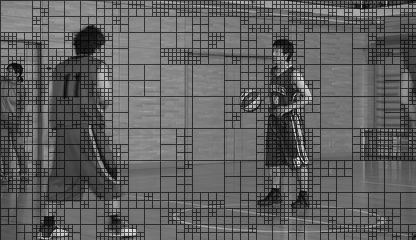
\includegraphics[width=0.5\linewidth]{./figures/partitioning-orig-all-001.png}}
	\\
	\subfloat[Predicted Image]
	{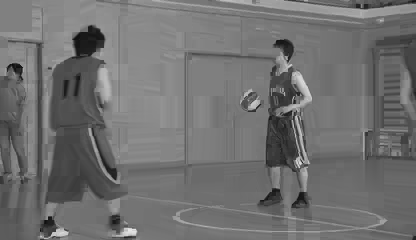
\includegraphics[width=0.5\linewidth]{./figures/pred_image-all-001.png}}
	\\
	\subfloat[Residual Image]
	{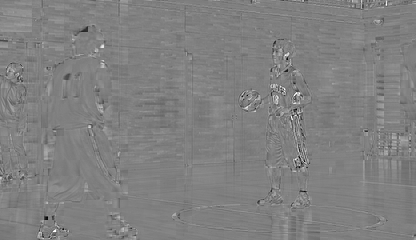
\includegraphics[width=0.5\linewidth]{./figures/res_image-all-001.png}}
	\caption{Example of an image at different encoding points for a
	certain level of quantisation}
	\label{fig:part_orig_pred_res_image}
\end{figure}

\subsubsection{Intra prediction}
\label{ssub:intra_prediction}
\index{intra prediction}

Intra prediction, sometimes referred to as spatial prediction, is used to
eliminate spatial redundancies by removing the correlation within local
regions of a picture.
The basic principle of intra prediction is based on the fact that the texture
of a picture region is similar to the texture of its neighbourhood and can be
predicted from there.
Images coded using this technique exclusively are named I-frames.

Different models of predictions can be used through projections of adjacent
decoded blocks.
These models include directional projections, gradient projections (called
Planar) and the projection of the mean value (called DC).
The \acp{IPM} are used to derive the predictions of the current block from its
the available boundaries, formed by reconstructed blocks.

\subsubsection{Inter prediction}
\label{ssub:inter_prediction}
\index{inter prediction}

Inter prediction, or temporal prediction, takes advantage of the fact that
consecutive images share many similarities, and that some of their component
regions will move as a whole.
Since the encoding order is not necessarily the same as the viewing one, inter
predictions can have their origins in either past or future frames, and also
combine both origins.
This feature facilitates movement tracking across frames.
Images that are predicted using only one image either from the past or from
the future are called predicted images or P-frames.
Bi-predicted images or B-frames have prediction origins in two different
images.

At the encoder side, an extra operation, called motion estimation, is
carried out.
This stage searches the best matching area in the reference picture for the
current prediction block.
It is one of the most complex parts of video coders in terms of computational
requirements.
Once a good prediction has been found, a motion vector is created, indicating
the offset that has to be applied in the block from the reference image.

\subsection{Transform}
\label{sub:transform}
\index{transform}
\index{energy compaction}

The transform stage reduces the remaining correlations from the residual
block, computed as the difference between the original and the predicted
blocks.
The goal of the transform is to concentrate the residual signal into as few
coefficients as possible in the transform domain.
The residual signal is transformed from the spatial domain using the
transform to the transform or frequency domain.
In the spatial domain, the residual signal is spread among the pixels of the
blocks, while the objective of transform domains is to concentrate as much as
possible the residual signal into a few transform domain coefficients
exhibiting a large amplitude and the rest might be considered negligible.

This idea of the energy compaction is the main property of the transform
stage.

Most of the transforms used in standardised video coding schemes belong to the
\ac{DTT} family.
Amongst those, the \ac{DCT} of type II has received a considerable amount of
attention in the past and is the \emph{de facto} standard transform used in
\acs{ITU} and \acs{MPEG} codecs since \acs{MPEG}-1/H.261.

Additional choices were introduced recently, especially in \ac{HEVC}, where
the \ac{DST} of type VII was adopted.

Provided that the subject of this thesis is centred around the
transforms for video coding, the transform stage will be explained
thoroughly in Chapter~\ref{cha:transform_coding}.

\subsection{Quantisation}
\label{sub:quantisation}
\index{QP}
\index{quantisation}
\index{lossy}
\index{lossless}

The quantisation, applied in the transform domain, is used as an approximation
operator, reducing the amount of possible output values.
In standards like \ac{HEVC}, the quantisation is scalar:
each coefficient is approximated independently from its neighbouring values.
In these coding schemes, the quantisation step is controlled by a \ac{QP} that
discards any coefficient whose energy level is below a certain threshold.
High energy coefficients are also affected by the quantisation.
It is worth noticing that the quantisation is the only non-reversible step in
the whole hybrid video coding scheme, which induces lossy video coding.
Lossless (or near-lossless) video coding can be attained by not using
quantisation in the process.

\subsection{Entropy coding}
\label{sub:entropy_coding}
\index{entropy coding}
\index{CABAC}
\index{scanning}

The last operation consists in reducing the amount of bits transmitted through
the use of an entropy code.
This is a lossless operation, as such the bit reduction performed during this
stage is reversible: no approximation operation is performed at this stage.

Once the transform coefficients have been quantised, they are scanned to make
sure they are sorted in a way that will make the entropy coder work
efficiently.

The scanning operation is a conversion from a 2D array, containing the
quantised transformed coefficients, towards a 1D vector containing the same
values sorted in a way that facilitates a compact transmission.
An appropriate scanning is crucial for efficient entropy
coding~\cite{ye-08-intra-directional-scanning-mddt}.

Signalling is also conveyed into the bitstream at this point, and the
entropy coder ensures a correct binarisation while using the adequate
number of bits thanks to the \ac{CABAC}.

\subsection{Intra coding in \acs{HEVC}}
\label{sub:intra_coding_in_hevc}
\index{PU}
\index{TU}
\index{scanning}

This subsection explains some particularities of the intra coding inside
\ac{HEVC}.

With regards to previous standards, such as \ac{AVC}, which has 9 different
prediction modes for intra coding, \ac{HEVC} has an improved prediction
system, with 35 different prediction modes.
The upper-left part of figure~\ref{fig:mdcs} illustrates them.
A detailed explanation on how predictions are derived from the block
boundaries using those prediction modes can be found in Chapter 6
of~\cite{wien-15-hevc}.

Depending on the selected \ac{IPM}, residuals present different patterns, and
so do their transformed coefficients.
The top-right part of figure~\ref{fig:mdcs} presents the average \ac{HEVC}
$4\times4$ residuals by scanning mode, together with their average
representation in transform domain through the \acs{DST}-VII.
The average residual profiles have lower (dark) values near the available
borders, which increase with the distance from the boundaries: residuals
issued from horizontal and vertical \acp{IPM} only have the left and upper
borders available, respectively, whereas the remaining \acp{IPM} tend to have
both borders available.
It can also be observed that the scanning patterns match reasonably well the
transformed coefficients in each case, sorting them in an increasing order.

These patterns in the transform domain determine different scanning orders (in
different colours), as presented in the lower part of figure~\ref{fig:mdcs}.
An adapted mode to each pattern ensures, in average, a correct order of the
coefficients that will group all the null values together.
The patterns are described for $4\times4$ blocks, and the same pattern is used
on higher block sizes, which are recursively split into 4 sub-blocks until
size $4\times4$ is reached~\cite{sole-12-transform-coefficient-coding}.

\begin{figure}[tb]
	\centering
	\begin{minipage}{0.48\textwidth}

		\ifthenelse{\usepdfs = 0}
		{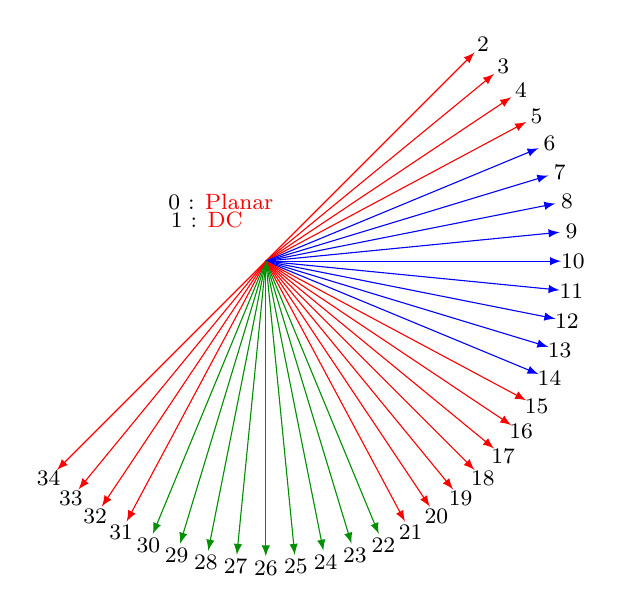
\begin{tikzpicture}[scale=1.5]

    \def\startx{0}
    \def\starty{0}
    \def\radius{2.5}
    \def\startangle{45}
    \def\colour{red}

    \draw (-0.38, 0.5) node {\footnotesize 0 : \color{red}{Planar}};
    \draw (-0.50, 0.5) node[below] {\footnotesize 1 : \color{red}{DC}};

    \foreach \direction in {2,3,...,34}
    {%
        % set the angle of current prediction direction 
        \pgfmathsetmacro{\angle}{\startangle - (\direction - 2) * 180 / 32}
        % horizontal directions (vertical scanning)
        \ifthenelse{\direction > 5 \AND \direction < 15}{\def\colour{blue}};
        % vertical directions (horizontal scanning)
        \ifthenelse{\direction > 21 \AND \direction < 31}{\def\colour{mygreen}};
        % draw the prediction direction lines with the appropriate colour
        \draw[-latex,\colour, thin] (\startx,\starty) --++ (\angle:\radius);
        % label each prediction direction
        \draw(\angle:\radius + 0.1) node {\footnotesize \direction};
    }

\end{tikzpicture}
}
		{\includegraphics{./figures/pred-directions.pdf}}
	\end{minipage}
	\begin{minipage}{0.48\textwidth}
		\centering
		\small
		Average profile for residuals (prediction direction)
		\begin{tabular}[H]{ccc}
			
\includegraphics[width=0.25\textwidth]{figures/resids-scan-diag.png}
			&
			
\includegraphics[width=0.25\textwidth]{figures/resids-scan-horz.png}
			&
			
\includegraphics[width=0.25\textwidth]{figures/resids-scan-vert.png}
			\\
			\color{red}{diagonal} & \color{greenish}{vertical} & \color{blue}{horizontal} \\
			& & \\
		\end{tabular}
		\\
		\small
		Average profile for coefficients (scanning mode)
		\begin{tabular}[H]{ccc}
			
\includegraphics[width=0.25\textwidth]{figures/coeffs-scan-diag.png}
			&
			
\includegraphics[width=0.25\textwidth]{figures/coeffs-scan-horz.png}
			&
			
\includegraphics[width=0.25\textwidth]{figures/coeffs-scan-vert.png}
			\\
			\color{red}{diagonal} & \color{greenish}{horizontal} & \color{blue}{vertical} \\
		\end{tabular}
	\end{minipage}
	\subfloat[Diagonal scanning]
	{\ifthenelse{\usepdfs = 0}
	{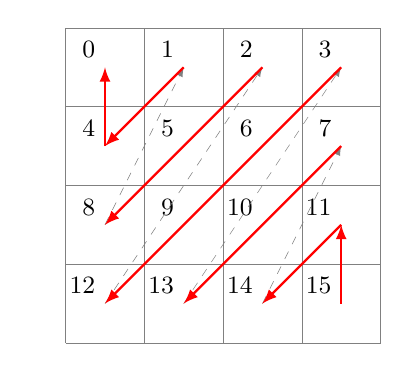
\begin{tikzpicture}[scale=1]

\def \xmax{4}
\def \ymax{4}
\draw[style=help lines, ystep=1, xstep=1]
	(0,0) grid (\xmax,\ymax);

\foreach \y in {0.5,1.5,...,\ymax}
{%
    \foreach \x in {0.5,1.5,...,\xmax}
    {%
      % floor the positions, as they are .5 and reverse vertical order
      \pgfmathtruncatemacro{\posX}{\x}
      \pgfmathtruncatemacro{\posY}{\ymax-\y}
      % calculate the index for each position
      \pgfmathtruncatemacro{\index}{\posX + \xmax * \posY}
      \node[above left] at (\x,\y){\small$\quad\;\index$};
    }
}



\def\startx{0.5}
\def\starty{3.5}

% help lines
\draw[-latex,style=help lines, dashed] (\startx + 0,\starty - 2) --++ (1,2);
\draw[-latex,style=help lines, dashed] (\startx + 0,\starty - 3) --++ (2,3);
\draw[-latex,style=help lines, dashed] (\startx + 1,\starty - 3) --++ (2,3);
\draw[-latex,style=help lines, dashed] (\startx + 2,\starty - 3) --++ (1,2);

% scanning
\draw[-latex,red,thick] (\startx + 0,\starty - 1) --++ ( 0, 1);
\draw[-latex,red,thick] (\startx + 1,\starty - 0) --++ (-1,-1);
\draw[-latex,red,thick] (\startx + 2,\starty - 0) --++ (-2,-2);
\draw[-latex,red,thick] (\startx + 3,\starty - 0) --++ (-3,-3);
\draw[-latex,red,thick] (\startx + 3,\starty - 1) --++ (-2,-2);
\draw[-latex,red,thick] (\startx + 3,\starty - 2) --++ (-1,-1);
\draw[-latex,red,thick] (\startx + 3,\starty - 3) --++ ( 0, 1);




\end{tikzpicture}
% vim:set filetype=tex et:
}
	{\includegraphics{figures/mdcs-diag.pdf}}}
	\subfloat[Horizontal scanning]
	{\ifthenelse{\usepdfs = 0}
	{\definecolor{greenish}{RGB}{0,145,0}
\begin{tikzpicture}[scale=1]
\def \xmax{4}
\def \ymax{4}
\draw[style=help lines, ystep=1, xstep=1]
	(0,0) grid (\xmax,\ymax);

\foreach \y in {0.5,1.5,...,\ymax}
{%
    \foreach \x in {0.5,1.5,...,\xmax}
    {%
      % floor the positions, as they are .5 and reverse vertical order
      \pgfmathtruncatemacro{\posX}{\x}
      \pgfmathtruncatemacro{\posY}{\ymax-\y}
      % calculate the index for each position
      \pgfmathtruncatemacro{\index}{\posX + \xmax * \posY}
      \node[above left] at (\x,\y){\small$\quad\;\index$};
    }
}

\def\startx{0.5}
\def\starty{3.5}

% help lines
\draw[-latex,style=help lines, dashed] (\startx + 0,\starty - 1) --++ (3,1);
\draw[-latex,style=help lines, dashed] (\startx + 0,\starty - 2) --++ (3,1);
\draw[-latex,style=help lines, dashed] (\startx + 0,\starty - 3) --++ (3,1);

% scanning
\draw[latex-,greenish,thick] (\startx,\starty - 0) --++ ( 3,0);
\draw[latex-,greenish,thick] (\startx,\starty - 1) --++ ( 3,0);
\draw[latex-,greenish,thick] (\startx,\starty - 2) --++ ( 3,0);
\draw[latex-,greenish,thick] (\startx,\starty - 3) --++ ( 3,0);

\end{tikzpicture}
}
	{\includegraphics{figures/mdcs-horz.pdf}}}
	\subfloat[Vertical scanning]
	{\ifthenelse{\usepdfs = 0}
	{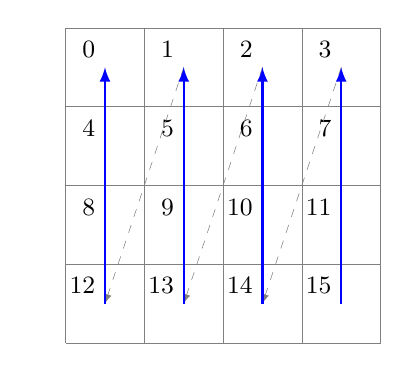
\begin{tikzpicture}[scale=1]

\def \xmax{4}
\def \ymax{4}
\draw[style=help lines, ystep=1, xstep=1]
	(0,0) grid (\xmax,\ymax);

\foreach \y in {0.5,1.5,...,\ymax}
{%
    \foreach \x in {0.5,1.5,...,\xmax}
    {%
      % floor the positions, as they are .5 and reverse vertical order
      \pgfmathtruncatemacro{\posX}{\x}
      \pgfmathtruncatemacro{\posY}{\ymax-\y}
      % calculate the index for each position
      \pgfmathtruncatemacro{\index}{\posX + \xmax * \posY}
      \node[above left] at (\x,\y){\small$\quad\;\index$};
    }
}

\def\startx{0.5}
\def\starty{3.5}

% help lines
\draw[-latex,style=help lines, dashed] (\startx + 1,\starty + 0) --++ (-1,-3);
\draw[-latex,style=help lines, dashed] (\startx + 2,\starty + 0) --++ (-1,-3);
\draw[-latex,style=help lines, dashed] (\startx + 3,\starty + 0) --++ (-1,-3);

% scanning
\draw[latex-,blue,thick] (\startx + 0,\starty) --++ ( 0,-3);
\draw[latex-,blue,thick] (\startx + 1,\starty) --++ ( 0,-3);
\draw[latex-,blue,thick] (\startx + 2,\starty) --++ ( 0,-3);
\draw[latex-,blue,thick] (\startx + 3,\starty) --++ ( 0,-3);

\end{tikzpicture}
}
	{\includegraphics{figures/mdcs-vert.pdf}}}
	\caption[\acs{HEVC} intra prediction modes and scannings for $4\times4$\acsp{TU}]
	{\acs{HEVC} \aclp{IPM} related to their average residual signals and their
	appropriate scanning in the transform domain for $4\times4$ \acsp{TU}}
	\label{fig:mdcs}
\end{figure}

\section{Encoder control}
\label{sec:encoder_control}
\index{encoder control}
\index{Lagrange}

The encoder control is used by essentially all blocks in the diagram
from figure~\ref{fig:hybrid_video_coding_scheme}.
This set of operations allows the encoder to take decisions related to coding
based on the application requirements.
These decisions include the block sizes and the prediction to use.
For each block size and type of prediction, the encoder computes the
distortion, using its own decoder, and estimates the rate as illustrated in
figure~\ref{fig:rate_distortion_scheme}.

The appropriate set of choices, mainly among the prediction modes and block
sizes, is performed by comparing the Lagrange values, which balance the
distortion and rates obtained for each coding choice.

Depending on the coding configuration, the encoder may also decide whether to
use references from the current image or from other images.
The \ac{AI} configuration, encodes each image independently from the rest,
whereas in the \ac{RA} configuration, the images conforming the sequences are
organised into \acp{GOP}, formed by an I-frame, and several P and B-frames.

\begin{figure}[tb]
	\centering
	\ifthenelse{\usepdfs = 0}
	{% \documentclass{book}
% \usepackage{tikz}
% \usepackage{mathptmx}
% \usepackage[scaled=0.92]{helvet}
% \begin{document}

\pgfmathsetmacro{\nodebasesize}{1} % A node with a value of one will have this diameter
\pgfmathsetmacro{\nodeinnersep}{0.1}

\newcommand{\propnode}[5]{% position, name, options, value, label
	\pgfmathsetmacro{\minimalwidth}{sqrt (#4*\nodebasesize)}
	\node[#3,minimum width=\minimalwidth*1cm,inner sep=\nodeinnersep*0cm,circle,draw]
	(#2) at (#1) {#5};
}

\tikzstyle{bloq} = [rectangle, draw, text badly centered, minimum height=2.5em, inner sep=1mm]
\newcommand{\bloq}[4]{% position, name options, label
	\node[bloq,#3] (#2) at (#1) {\textsf{#4}};
}
\newcommand{\add}[2]{%position, name
	\draw (4,4) circle [radius=0.3] node (add) {\textsf$+$};
}

\begin{tikzpicture}[scale=1.5, x=1em, y=1em]
\tikzstyle{every node}=[font=\small]

	\def\startx{0}
	\def\starty{0}
	\def\thickness{thick}
	\def\hdist{5}
	\def\vdist{3}

	\filldraw[fill=blue!20, draw=blue!50,dashed,thick]
	(\startx-2.5,\starty+2) --++ (15,0) --++ (0,-4) --++ (-15,0) -- cycle;
	\filldraw[fill=blue!20, draw=blue!50,dashed,thick]
	(\startx-2.5,\starty-\vdist-1) --++ (15,0) --++ (0,-4) --++ (-15,0) -- cycle;

	\bloq{\startx+0*\hdist,\starty-0*\vdist}{transf}{text width=5.0em,fill=yellow!50}{\textsf{transform}}
	\bloq{\startx+1*\hdist,\starty-0*\vdist}{quant}{text width=5.0em,fill=yellow!50}{\textsf{quantisation}}
	\bloq{\startx+2*\hdist,\starty-0*\vdist}{entrocod}{text width=5.0em,fill=yellow!50}{\textsf{entropy coding}}

	\bloq{\startx+2*\hdist,\starty-2*\vdist}{entrodec}{text width=5.0em,fill=yellow!50}{\textsf{entropy decoding}}
	\bloq{\startx+1*\hdist,\starty-2*\vdist}{iquant}{text width=5.0em,fill=yellow!50}{\textsf{inverse quantisation}}
	\bloq{\startx+0*\hdist,\starty-2*\vdist}{itransf}{text width=5.0em,fill=yellow!50}{\textsf{inverse transform}}

	\node (rate) at (\startx+3*\hdist,\starty-1*\vdist) {\textsf{rate}};
	\node [label={[xshift=0cm, yshift=0.5cm]\textsf{encoder}}] at (quant) {};
	\node [label={[xshift=0cm, yshift=-1.2cm]\textsf{decoder}}] at (iquant) {};

	\draw[latex-, \thickness] (transf) -- (-4,0) node [left] (in) {\large$x$};
	\draw[-latex, \thickness] (itransf) -- (-4,-2*\vdist) node [left] (out) {\large$\hat x$};

	\node (dist) at (-4.425,-\vdist) {\textsf{distortion}};

	\draw [-latex, \thickness] (dist) -- (in);
	\draw [-latex, \thickness] (dist) -- (out);

	\draw[-latex, \thickness] (transf) -- (quant);
	\draw[-latex, \thickness] (quant) -- (entrocod);
	\draw[\thickness] (entrocod) -| (rate);
	\draw[-latex, \thickness] (rate) |- (entrodec);
	\draw[-latex, \thickness] (entrodec) -- (iquant);
	\draw[-latex, \thickness] (iquant) -- (itransf);


\end{tikzpicture}
% \end{document}
}
	{\includegraphics{./figures/rate_distortion_scheme.pdf}}
	\caption{Rate-distortion scheme of a transform-based codec}
	\label{fig:rate_distortion_scheme}
\end{figure}

\subsection{Distortion measures}
\label{sub:distortion_measures}

\subsubsection{Mean squared error}
\label{ssub:mean_squared_error}
\index{MSE}

The \ac{MSE} is the average of the square difference between two
signals.
For two-dimensional signals, such as images, the \ac{MSE} can be computed as:
\begin{equation}
	MSE_{I,K} = \frac{1}{m\,n} \sum\limits_{i=0}^{m-1} \sum\limits_{j=0}^{n-1}
	{\left[ I(i,j) - K(i,j) \right]} ^2
	\label{eqn:mse}
\end{equation}
Where $I$ and $K$ are two images of $m \times n$ pixels.
Usually, $I$ is the reference image and $K$ the coded image.

\subsubsection{Peak signal-to-noise ratio}
\label{ssub:peak_signal_to_noise_ratio}
\index{PSNR}

The \ac{PSNR} is an objective measure of quality that computes the ratio
between the maximum possible value of a signal and the energy of the noise
that affects the fidelity of its approximation.
It is usually defined in a logarithmic scale to cope with the wide range that
signals might have.
Defining the \ac{PSNR} in terms of the \ac{MSE} from~\eqref{eqn:mse}, it can
be expressed as:
\begin{equation}
	PSNR = 10 \log_{10} \left(\frac{MAX_I^2}{MSE_{I,K}}\right)
	= 20 \log_{10} (MAX_I) - 10 \log_{10} (MSE_{I,K})
	\label{eqn:psnr}
\end{equation}
For 8-bit depth images, which are the main format considered in this thesis,
the maximum pixel values writes: $MAX = 2^{8} - 1 = 255$.

\subsection{Rate-distortion optimisation}
\label{sub:rate_distortion_optimisation}
\index{RDO}
\index{Lagrange}

In order to carry out the most sensible decision each time, the encoder uses a
\ac{RDO} criterion~\cite{sullivan-98-rdo-video-compression}.

Each time the encoder has to make a decision about choosing a
particular block size for the partitioning or a prediction mode, it
checks the distortion that decision might cause as well as an estimation
of the bit-rate needed.
The encoder performs this computation iteratively on the same block,
exploring many different coding possibilities and finally selects the
one that provides the best score in terms of rate and distortion.
This is called the \ac{RDO} loop.
For instance, in \ac{HEVC}, it allows choosing the best \ac{PU} size
(4,8,16,32,64), \ac{TU} size (4,8,16,32), \ac{IPM} (0,1,\ldots,34), prediction
source (intra, inter), amongst others.

The trade-off between the distortion and the rate is commonly expressed
using a Lagrange measure.

\begin{equation}
	J(\lambda) = \text{Distortion} + \lambda \text{Rate}
	\label{eqn:lagrangian_rdo}
\end{equation}

As seen in the previous subsections, computing the distortion is
reasonably straightforward.
However, estimating the bit-rate is a bit more delicate, since the whole
entropy coder cannot be run each time the encoder explores the different
possibilities for a block because it has a huge impact on complexity.
As a consequence, an estimation of the bit-rate is often used in the \ac{RDO}
loop.

\section{Bj{\o}ntegaard Delta measurements}
\label{sub:bjontegaard_delta_measurements}
\index{BD-rate}
\index{BD-PSNR}

Comparing two video coding techniques objectively might be complicated,
as both the distortion and the bit-rate savings have to be taken into account
jointly.

Metrics introduced by Gisle Bjøntegaard, know as \ac{BD} measurements have
become the current \emph{de facto} procedure to objectively compare the result
of two encodings~\cite{VCEG-M33,VCEG-AI11}.
Two different metrics are defined and displayed in
figure~\ref{fig:bdsnr_bdrate}:
\begin{enumerate}[label = (\alph{enumi})]
	\item \ac{BD}-\ac{PSNR}: computes the relative quality improvement
		in \si{\decibel}.
	\item \ac{BD}-rate: computes the relative savings in bit-rate for an
		equivalent distortion in percent.
\end{enumerate}

\begin{figure}[tb]
	\centering
	\subfloat[\acs{BD}-\acs{PSNR}]
	{\ifthenelse{\usepdfs = 0}
	{\begin{tikzpicture}
	\pgfplotsset{/tikz/font={\small}}
	\begin{axis}[
			% title=Bitrate savings: $-8.94\%$. SNR improvement: $0.46$ dB,
			xlabel={Bitrate (Mbps)},
			ylabel={PSNR Y (dB)},
			grid=both,
			scale only axis,
			width=0.375\textwidth,
			height=0.25\textheight,
			xtick={0,3,...,21},
			x tick label style={
				/pgf/number format/.cd,
				fixed,
				fixed zerofill,
				precision=0,
			},
			scaled x ticks=false,
			ytick={32,33,...,45},
			y tick label style={
				/pgf/number format/.cd,
				fixed,
				fixed zerofill,
				precision=0,
				/tikz/.cd
			},
			xmin=0, xmax=21,
			ymin=32, ymax=43,
			legend style={nodes=right},
			legend pos= south east
		]
		\addplot [name path=refsnr, blue, thick] table {
		3.35	32.76
		6.07	35.40
		11.31	38.37
		19.81	41.40
		};

		\addplot [name path=expsnr, red, thick] table {
		3.35	33.60
		5.58	35.95
		10.75	38.93
		19.81	42.18
		};
		\addplot [black, thin] table {
		3.35	32.76
		3.35	33.60
		};
		\addplot [black, thin] table {
		19.81	41.40
		19.81	42.18
		};

		\addplot[gray!33] fill between[ of = refsnr and expsnr];

		\addplot [name path=ref, mark=*,mark size=1pt, blue, thick] table {
		3.35	32.76
		6.07	35.40
		11.31	38.37
		20.81	41.76
		};
		\addlegendentry{REF}
		\addlegendentry{EXP}
		\addplot [name path=exp, mark=*,mark size=1pt, red, thick] table {
		3.00	33.24
		5.58	35.95
		10.75	38.93
		19.81	42.18
		};
	\end{axis}
\end{tikzpicture}
}
	{\includegraphics{./figures/bd_psnr_plot.pdf}}}
	\hfill
	\subfloat[\acs{BD}-rate]
	{\includegraphics{./figures/bd_rate_plot.pdf}}
	\caption{Schematic representation of rate-distortion plots using the
	\acs{BD} measurements}
	\label{fig:bdsnr_bdrate}
\end{figure}

The \ac{BD}-rate measurement is extensively used in this thesis to
appreciate the performance of the proposed systems, as it is the metric used
by \acs{JCT-VC} in standardisation.

\section{Conclusions}
\label{sec:conclusions_video_coding}

This Chapter has presented the motivation for video compression as well as
some general concepts concerning an overview of the video coding system.

Current video coders exploit redundancies existing within images of the video
sequence via predictions.
These predictions can be either spatial or temporal, depending respectively on
whether the prediction source is the same image or another image.
Unpredictable parts of the image, called residuals, are then passed through a
transformation step in order to concentrate the transformed residual into as
few coefficients as possible.

The appropriate block size is selected for the prediction and the transform
sizes, named \acp{PU} and \acp{TU}, respectively.
A lot of flexibility is allowed for the prediction and sizes while the set of
choices for a given codec is rather limited for the transform.

This thesis will focus on the extension of the choices for the transform
stage.
Currently, the decision of the coding configuration (\ac{AI}, \ac{RA}), the
block sizes and \acp{IPM} are is based on a single transform, usually the
\ac{DCT}-II.
However, a single transform is unlikely provide optimal signal compaction for
all kinds of possible signals.

This thesis focuses on the extension of the choices for the transform
stage, as set of transforms will be provided such that the encoder is able to
better adapt the transform to the varying nature of the prediction residuals.

Next chapter explores the details of the transforms used in video coding,
namely their design principles and a comparison between two design approaches.

\chapter{Transform coding}
\label{cha:transform_coding}
\chaptertoc

\section{Introduction to transforms}
\label{sec:introduction_to_transforms}
\index{transform}
\index{transform coding}
\index{rotation}

In the previous chapter, transforms were identified as an important part in
current video coding standards.
This chapter studies the design and properties that make transforms useful in
video coding.

A transform is a mathematical transfer function of a signal from a
representation domain to another.

The high energy compaction offered by transform process has led this technique
to be part of all the international video coding standards.

Transforms allow reducing existing signal correlations in the spatial domain,
leading to a more decorrelated signal in the transform domain and ensuring a
more compact representation.
This is of great importance for the upcoming stages of scanning and entropy
coding.

Transforms can be very abstract since they tend to work in $N$-dimensional
spaces, where $N$ represents the number of pixel residuals processed by the
transform.
Typical values vary from $N=4\times4$ to $N=32\times32$ using powers of two in
modern video codecs, such as \ac{HEVC}.

However, restraining ourselves to the two-dimensional case, one of the most
visual and representative example of transforms are rotations.
The example in figure~\ref{fig:transform_rotation} helps visualising the
transform role in signal compression.

\begin{figure}[tb]
	\centering
	\ifthenelse{\usepdfs = 0}
	{% \documentclass{book}
% \usepackage{tikz, libertine, ifthen}
% \begin{document}
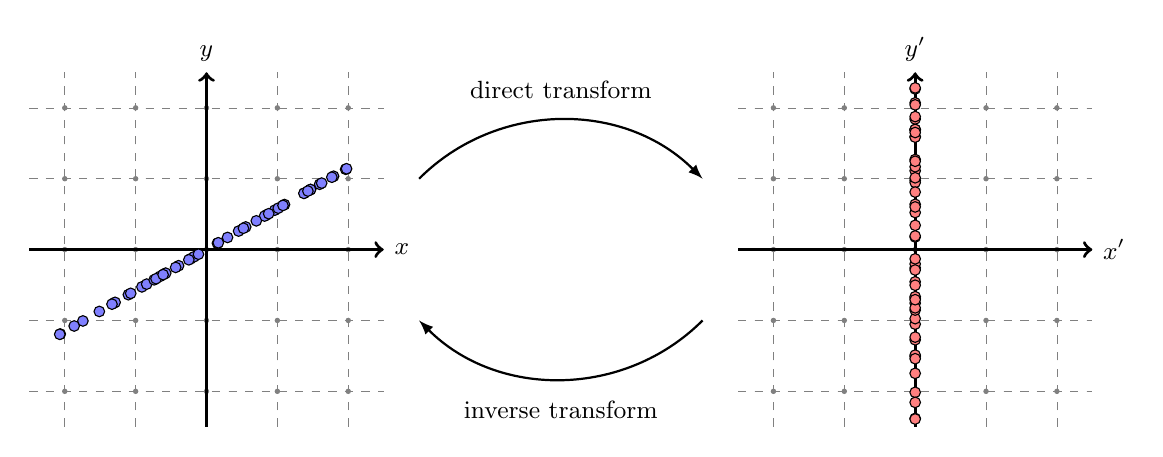
\begin{tikzpicture}[scale=0.9]
\tikzstyle{every node}=[font=\small]

	\draw[style=help lines, dashed, very thin, rotate=0] (0.5,0.5) grid (5.5,5.5);
	\draw[style=help lines, dashed, very thin, rotate=0] (10.5,0.5) grid (15.5,5.5);

	\foreach \x in {1,2,...,5} {
		\foreach \y in {1,2,...,5} {
			\filldraw [black!50, opacity = 1] (\x,\y) circle (0.03);
		}
	}

	\foreach \x in {11,12,...,15} {
		\foreach \y in {1,2,...,5} {
			\filldraw [black!50, opacity = 1] (\x,\y) circle (0.03);
		}
	}

	\def\seed{88}
	\pgfmathsetmacro{\xvar}{2.4}
	\pgfmathsetmacro{\yvar}{0.0}

	\def\angle{30}
	\pgfmathsetseed{\seed}
	\pgfmathsetmacro{\xoff}{3}
	\pgfmathsetmacro{\yoff}{3}
	\draw[style=help lines, dashed, very thin, rotate=0]
		(\xoff-2.5,\yoff-2.5) grid (\xoff+2.5,\yoff+2.5);
	\draw[->,very thick] (\xoff-2.5,\yoff)--(\xoff+2.5,\yoff) node[right]{$x$};
	\draw[->,very thick] (\xoff,\yoff-2.5)--(\xoff,\yoff+2.5) node[above]{$y$};
	\pgfmathsetmacro{\radius}{0.075}
	\foreach \i in {1,2,...,50} {
		\pgfmathsetmacro{\x}{(rand) * \xvar}
		\pgfmathsetmacro{\y}{(rand) * \yvar}
		\pgfmathsetmacro{\xrot}{\x*cos(\angle) - \y*sin(\angle) + \xoff}
		\pgfmathsetmacro{\yrot}{\x*sin(\angle) + \y*cos(\angle) + \yoff}
		\filldraw [black, fill=blue!50] (\xrot,\yrot) circle (\radius);
	}

	\def\angle{90}
	\pgfmathsetseed{\seed}
	\pgfmathsetmacro{\xoff}{13}
	\pgfmathsetmacro{\yoff}{3}
	\draw[style=help lines, dashed, very thin, rotate=0]
		(\xoff-2.5,\yoff-2.5) grid (\xoff+2.5,\yoff+2.5);
	\draw[->,very thick] (\xoff-2.5,\yoff)--(\xoff+2.5,\yoff) node[right]{$x'$};
	\draw[->,very thick] (\xoff,\yoff-2.5)--(\xoff,\yoff+2.5) node[above]{$y'$};
	\foreach \i in {1,2,...,50} {
		\pgfmathsetmacro{\x}{(rand) * \xvar}
		\pgfmathsetmacro{\y}{(rand) * \yvar}
		\pgfmathsetmacro{\xrot}{\x*cos(\angle) - \y*sin(\angle) + \xoff}
		\pgfmathsetmacro{\yrot}{\x*sin(\angle) + \y*cos(\angle) + \yoff}
		\filldraw [black, fill=red!50] (\xrot,\yrot) circle (\radius);
	}

	\draw [thick,-latex] (6,4) to [in=135,out=45] ++ (4,0);
	\draw [thick,latex-] (6,2) to [in=-135,out=-45] ++ (4,0);
	\node [above] at (8,5) {direct transform};
	\node [below] at (8,1) {inverse transform};
\end{tikzpicture}
% \end{document}
}
	{\includegraphics{./figures/transform_rotation_plot.pdf}}
	\caption{Simple transform performing a rotation}
	\label{fig:transform_rotation}
\end{figure}

Whereas on the left signal (in blue), both coordinates are needed to describe
the signal accurately, on the right signal (in red), one coordinate, namely
the vertical dimension is enough to provide an equally accurate signal
representation, since the horizontal dimension remains constant.

\subsection{Block transforms}
\label{sub:block_transforms}
\index{block transforms}
\index{JPEG}
\index{HEVC}
\index{AVC}

Block-based coding is widely adopted in image/video systems, such as
\acs{JPEG}~\cite{jpeg}, \ac{AVC} and \ac{HEVC}.

In these systems, the image to be transformed is split into non-overlapping
blocks, and each one is treated and transformed
independently~\cite{xu-09-intra-predictive-transforms}.
This provides an advantage of being less expensive in terms of computing that
other kinds of transforms, such as wavelet transforms used in
\acs{JPEG}-2000~\cite{jpeg2000}.

Since \ac{HEVC} uses block transforms only, they will be used in this thesis
to build up new systems.

\subsection{Orthogonal transforms}
\label{sub:orthogonal_transforms}
\index{orthogonal transforms}
\index{orthonormal transforms}
\index{unitary transforms}

Transforms used in image processing and video coding systems are orthogonal.
Orthogonal matrices are square matrices whose rows and columns are orthogonal
unit vectors, also known as orthonormal vectors, with:
\begin{equation}
	\A^T\A = \A\A^T = \I
\end{equation}
As a consequence, the inverse matrix of an orthogonal matrix is its
transposed version:
\begin{equation}
	\A^T = \A^{-1}
\end{equation}

This property offers some benefits:
\begin{itemize}
	\item Fast computation of inverse transform with no need to store it
		separately.
	\item Re-use of fast algorithms for both direct and inverse transform
		applications.
	\item Energy preservation.
\end{itemize}

\subsection{Separability}
\label{sub:separability}
\index{separable transforms}

Image and video coding deal with image blocks, which are two-dimensional
signals and, consequently, use transforms able to process those signals.

The straightforward approach to work with those signals is to use
non-separable transforms.
These transforms take the residual pixels from a block previously reshaped
into a single-dimensional signal.
For instance, a $4\times4$ block of pixels becomes a $16\times1$ vector, as
illustrated in figure~\ref{fig:block_linearisation}.
Afterwards the transform is applied normally:
\begin{equation}
	\X = \A \, \x
\end{equation}
where $\x$ is a $N \times N$ block, reshaped into a $N^2\times1$ vector
and $\A$ is a $N^2 \times N^2$ matrix.
The main disadvantage of this approach is the number of calculations
required to obtain the transformed signal: for a $N \times N$ block, the
number of operations required to transform it in a non-separable way is:
$N^4$ multiplications and $N^2(N^2-1)$ additions.

\begin{figure}[tb]
	\centering
	\ifthenelse{\usepdfs = 0}
	{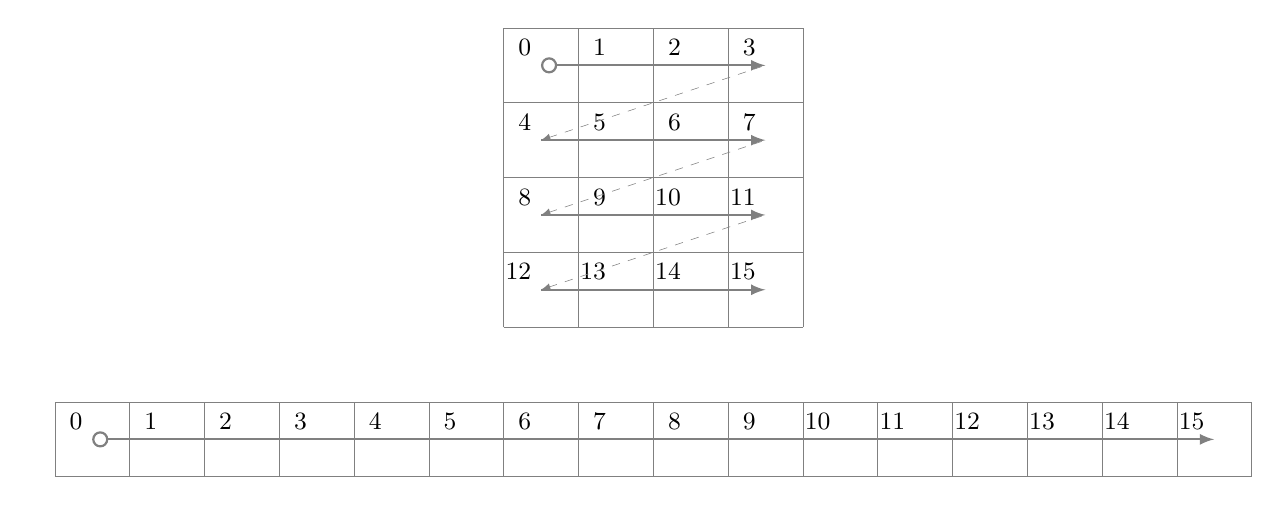
\begin{tikzpicture}[scale=0.95]

\def \xmax{4}
\def \ymax{4}
\draw[style=help lines, ystep=1, xstep=1]
	(0,0) grid (\xmax,\ymax);

\foreach \y in {0.5,1.5,...,\ymax}
{%
    \foreach \x in {0.5,1.5,...,\xmax}
    {%
      % floor the positions, as they are .5 and reverse vertical order
      \pgfmathtruncatemacro{\posX}{\x}
      \pgfmathtruncatemacro{\posY}{\ymax-\y}
      % calculate the index for each position
      \pgfmathtruncatemacro{\index}{\posX + \xmax * \posY}
      \node[above left] at (\x,\y){\small$\quad\;\index$};
    }
}

\def\startx{0.5}
\def\starty{3.5}

% help lines
\draw[latex-,style=help lines, dashed] (\startx + 0,\starty - 1) --++ (3,1);
\draw[latex-,style=help lines, dashed] (\startx + 0,\starty - 2) --++ (3,1);
\draw[latex-,style=help lines, dashed] (\startx + 0,\starty - 3) --++ (3,1);

% scanning
\draw[o-latex,style=help lines,thick] (\startx,\starty - 0) --++ ( 3,0);
\draw[-latex,style=help lines,thick] (\startx,\starty - 1) --++ ( 3,0);
\draw[-latex,style=help lines,thick] (\startx,\starty - 2) --++ ( 3,0);
\draw[-latex,style=help lines,thick] (\startx,\starty - 3) --++ ( 3,0);

\def \xmax{16}
\def \ymax{1}
\def\startx{-6}
\def\starty{-2}

\draw[style=help lines, ystep=1, xstep=1]
	(\startx,\starty) grid (\startx+\xmax,\starty+\ymax);
\foreach \x in {0,1,...,15}
{%
    \node[above left] at (\x+\startx+0.5,\starty+0.5) {\small$\quad\;\x$};
}

\draw[o-latex,style=help lines,thick] (\startx+0.5,\starty+0.5) --++ (\xmax-1,0);

\end{tikzpicture}

% vim:set filetype=tex et:
}
	{\includegraphics{./figures/block_linearisation.pdf}}
	\caption{Example of a $4\times4$ block linearisation}
	\label{fig:block_linearisation}
\end{figure}
\index{block linearisation}

On the other hand, any linear correlation can be exploited between any pixel
within a block:
complex relationships between distant pixels can be handled regardless their
position in the block.

Due to the high amount of operations needed to transform a block using
non-separable transforms, separable transforms are widely used in video
coding.
A block is transformed separately using horizontal and vertical transforms
$\A_h, \A_v$ for its rows and columns, respectively, as:
\begin{equation}
	\X = \A_v {\left(\A_h \, \x^T\right)}^T = \A_v \, \x \, \A_h^T
	\label{eqn:sep_transform}
\end{equation}
The operation inside the parenthesis transforms the rows of $\x$, and the
outer part, the columns of the result.
By performing the horizontal and vertical transforms separately, the number of
operations required is reduced to $2N^3$ multiplications and $2N^2(N-1)$
additions.

However, this reduction in complexity comes at a price:
non-separable transforms are able to exploit any correlation amongst pixels
within a block, whereas separable transforms can only decorrelate pixels that
share the same row or column.
In other words, separable transforms might be less efficient than their
non-separable counterparts.
The impact in performance due to separability will be studied in detail
in Chapter~\ref{cha:mddt}.

A non-separable transform can be expressed from a set of two separable
transforms via the Kronecker product, denoted as $\otimes$.
\begin{equation}
	\mathbf{A}\otimes\mathbf{B} =
	\begin{bmatrix}
		a_{11} \mathbf{B} & \cdots & a_{1n}\mathbf{B} \\
		\vdots & \ddots & \vdots \\
		a_{m1} \mathbf{B} & \cdots & a_{mn} \mathbf{B}
	\end{bmatrix}
\end{equation}
Where $\mathbf{A}$ is an $m \times n$ matrix and $\mathbf{B}$ is a $p \times
q$ matrix.
More explicitly:
\begin{equation}
	\mathbf{A}\otimes\mathbf{B} =
	\begin{bmatrix}
		a_{11} b_{11} & a_{11} b_{12} & \cdots & a_{11} b_{1q} & \cdots & \cdots & a_{1n} b_{11} & a_{1n} b_{12} & \cdots & a_{1n} b_{1q} \\
		a_{11} b_{21} & a_{11} b_{22} & \cdots & a_{11} b_{2q} & \cdots & \cdots & a_{1n} b_{21} & a_{1n} b_{22} & \cdots & a_{1n} b_{2q} \\
		\vdots & \vdots & \ddots & \vdots & & & \vdots & \vdots & \ddots & \vdots \\
		a_{11} b_{p1} & a_{11} b_{p2} & \cdots & a_{11} b_{pq} & \cdots & \cdots & a_{1n} b_{p1} & a_{1n} b_{p2} & \cdots & a_{1n} b_{pq} \\
		\vdots & \vdots & & \vdots & \ddots & & \vdots & \vdots & & \vdots \\
		\vdots & \vdots & & \vdots & & \ddots & \vdots & \vdots & & \vdots \\
		a_{m1} b_{11} & a_{m1} b_{12} & \cdots & a_{m1} b_{1q} & \cdots & \cdots & a_{mn} b_{11} & a_{mn} b_{12} & \cdots & a_{mn} b_{1q} \\
		a_{m1} b_{21} & a_{m1} b_{22} & \cdots & a_{m1} b_{2q} & \cdots & \cdots & a_{mn} b_{21} & a_{mn} b_{22} & \cdots & a_{mn} b_{2q} \\
		\vdots & \vdots & \ddots & \vdots & & & \vdots & \vdots & \ddots & \vdots \\
		a_{m1} b_{p1} & a_{m1} b_{p2} & \cdots & a_{m1} b_{pq} & \cdots & \cdots & a_{mn} b_{p1} & a_{mn} b_{p2} & \cdots & a_{mn} b_{pq} 
	\end{bmatrix}
\end{equation}
\index{Kronecker product}

\subsection{Transform design}
\label{sub:transform_design}
\index{transform design}

Since the objective of the transforms is to be able to represent the signal
with as few coefficients as possible while minimising the distortion
introduced by the quantisation, transform design methods need to consider
trade-offs between the distortion and the number of bits needed to represent
those signals in the transform domain, as shown previously in
\S\ref{sub:rate_distortion_optimisation}.

Most transform design methods use the \ac{MSE} from~\eqref{eqn:mse} to
evaluate the distortion introduced by a quantiser applied in the transform
domain.
However, different transform designs exist depending on how the bit-rate is
estimated and modelled.

Next sections will study different transform design approaches based on
different modellings of the rate constraint.
\section{The Karhunen-Loève transform}
\label{sec:the_karhunen_loeve_transform}
\index{KLT}
The components of source signals within a residual block tend to be correlated
amongst them.
This correlation is expressed in terms of a correlation matrix containing the
linear inter pixel correlations.
For two $N$-dimensional signals $\x,\y$, the covariance signal between them
can be computed as:
\begin{align}
	\nonumber
	\C_{\x,\y} & = \E\left\{\x\y^T\right\} =
	\E\left\{
	\begin{bmatrix}
		x_0 \\ x_1 \\ \vdots \\ x_{N-1}
	\end{bmatrix}
	\begin{bmatrix}
		y_0 & y_1 & \cdots & y_{N-1}
	\end{bmatrix}
	\right\} \\
	& = \E\left\{
	\begin{bmatrix}
		x_0y_0 & x_0y_1 & \hdots & x_{0}y_{N-1} \\
		x_1y_0 & x_1y_1 & \hdots & x_{1}y_{N-1} \\
		\vdots & \vdots & \ddots & \vdots \\
		x_{N-1}y_0 & x_{N-1}y_1 & \hdots & x_{N-1}y_{N-1}
	\end{bmatrix}
	\right\} \\ \nonumber
	& =
	\begin{bmatrix}
		\E\left\{x_0y_0\right\} & \E\left\{x_0y_1\right\} & \hdots & \E\left\{x_{0}y_{N-1}\right\} \\
		\E\left\{x_1y_0\right\} & \E\left\{x_1y_1\right\} & \hdots & \E\left\{x_{1}y_{N-1}\right\} \\
		\vdots & \vdots & \ddots & \vdots \\
		\E\left\{x_{N-1}y_0\right\} & \E\left\{x_{N-1}y_1\right\} & \hdots & \E\left\{x_{N-1}y_{N-1}\right\}
	\end{bmatrix}
\end{align}
\index{covariance matrix}
\index{correlation matrix}
If $\x=\y$, the covariance matrix is the correlation matrix of $\x$.

It is possible to select an orthogonal matrix $\A$ that will make $\X=\A\x$
have pairwise uncorrelated components in the transform
domain~\cite{gersho-92-vector-quantization}.
The \ac{KLT} is defined as the linear orthogonal transform that reduces the
redundancy by a maximum decorrelation of the data, so that the signal can be
stored more efficiently~\cite{rao-01-transform-data-compression-book}.

In this section, the \ac{KLT} is presented under its well-known optimal
condition:
the high-resolution quantisation assumption~\cite{goyal-00-high-resolution}.
The high-resolution assumption states that the number of quantisation levels
is high and the quantisation step size is small enough to consider the
\ac{PDF} constant for each quantisation interval.

Under this condition, the \ac{KLT} is the transform that achieves optimal
bit allocation for the quantisation of transform coefficients by distributing
their variances in such a way as to minimise their geometric
mean~\cite{jayant-84-digital-coding-waveforms}, while minimising the overall
distortion~\cite{gersho-92-vector-quantization}.

The \ac{KLT} decorrelates the signal in the transform domain, that is the
correlation function of the signal in the transform domain $\C_\X$ is a
diagonal matrix, which can be computed as follows.
Let $\x$ be a zero-mean process and $\A$ an orthogonal transform, then, in
the transform domain:
\begin{equation}
	\X = \A \x \qquad \text{s.t. } \A \A^T = \I
\end{equation}
The covariance matrix in the transform domain is expressed as:
\begin{equation}
	\C_\X = \E\left\{\X \X^T\right\} = \A \E\left\{\x\x^T\right\}\A^T =
	\A\C_\x\A^T
\end{equation}
Or equivalently:
\begin{equation}
	\A^T\C_\X = \C_\x\A^T
\end{equation}
And since $\C_\X$ is diagonal:
\begin{equation}
	\C_\x \a_i = \lambda_i\a_i
\end{equation}
Where:
\begin{itemize}
	\item $\a_i$'s are the eigenvectors of $\C_\x$.
	\item $\lambda_i$'s are the eigenvalues of $\C_\x$.
\end{itemize}
\index{eigen values}
\index{eigen vectors}

As a result, the \ac{KLT} is a transform whose base vectors are the
eigenvectors of the correlation matrix of the input signal.

\subsection{Particular case on natural images: the \acs{DCT}}
\label{sub:particular_case_dct}
\index{DCT}
\index{Markov}
\index{AR}

One of the most used transforms in image and video coding is the
\acf{DCT}.
In this section, the \ac{DCT} is justified over a particular kind
of signals: natural images.
The statistics of pixels in natural images match closely a first order
\ac{AR} process.
A first order \ac{AR} model, also known as Markov-1 process, is a stochastic
process that can be generated through the following regression formula:
\begin{equation}
	x(n) = \rho x(n-1) + w(n)
	\label{eqn:first_order_ar_model}
\end{equation}
Where $\rho$ is the correlation coefficient between two adjacent samples
and $w(n)$ is a white noise with zero mean, whose variance is related to
the variance of $x(n)$ $\sigma_x^2$ as:
\begin{equation}
	\sigma_w^2 = \E\left\{ w(n) w(n) \right\} =
	\left(1-\rho^2\right)\sigma_x^2
\end{equation}
The correlation matrix of this process takes the form of a Toeplitz
matrix~\cite{akansu-12-toeplitz-approximation}:
\begin{equation}
	\R_x = \sigma_x^2
	\begin{pmatrix}
		1          & \rho       & \rho^2     & \cdots & \rho^{N-1} \\
		\rho       & 1          & \rho       & \cdots & \rho^{N-2} \\
		\rho^2     & \rho       & 1          & \cdots & \rho^{N-3} \\
		\vdots     & \vdots     & \vdots     & \ddots & \vdots     \\
		\rho^{N-1} & \rho^{N-2} & \rho^{N-3} & \cdots & 1
	\end{pmatrix}
	\label{eqn:toeplitz_matrix}
\end{equation}
\index{Toeplitz matrix}
The \ac{KLT} for this kind of processes, that is, the eigenvectors of
$\R_\x$, tends to the \ac{DCT} as $\rho\to1$~\cite{britanak-06-dct-and-dst}.
The \ac{DCT}-II can be expressed compactly as:
\begin{equation}
	{\left[C_{N}^{II} \right]}_{n,k} =
	\sqrt{\frac{2}{N}}\epsilon_k\cos\left(\frac{\pi(2n+1)k}{2N}\right)
	\quad
	n,k=0,\dots,N-1
	\label{eqn:dct_ii}
\end{equation}

\begin{equation}
	\epsilon_k =
	\begin{cases}
		\frac{1}{\sqrt{2}} & k = 0 \\
		1 & \text{otherwise}
	\end{cases}
\end{equation}

The fact that the \ac{DCT} approximates the \ac{KLT} for image signals and its
efficient implementation has made it the preferred choice in image and video
compression algorithms to decorrelate the signals and provide optimal bit
allocation~\cite{sole-12-transform-coefficient-coding}.

\begin{figure}[tb]
	\centering
	\subfloat[\acs{DCT}-II $4\times4$]
	{
\includegraphics[width=0.3\linewidth]{./figures/dct4-bases.png}}
	\hspace{0.2\linewidth}
	\subfloat[\acs{DST}-VII $4\times4$]
	{
\includegraphics[width=0.3\linewidth]{./figures/dst4-bases.png}}
	\caption{Transforms used in \acs{HEVC} for $4\times4$ blocks}
	\label{fig:dct_dst}
\end{figure}

\subsection{Particular case on prediction residuals: the \acs{DST}}
\label{sub:particular_case_dst}
\index{DST}
\index{intra prediction}
\index{Toeplitz matrix}

Although the \ac{DCT} has been proved to be nearly the \ac{KLT} for natural
images, it is used in predictive transform coding based video standards.
This kind of coding leads to signals whose nature differs from that of
natural images: prediction residuals.
More precisely, prediction residuals resulting from intra prediction tend to
have particular properties.
Those residuals are computed using predictions from already
reconstructed blocks, usually available on the left and upper borders (in
grey) of the current residual (in white), as shown in
figure~\ref{fig:pred_scheme}.a.
An example of an average intra prediction residual is provided in
figure~\ref{fig:pred_scheme}.b.
It can be noticed that the energy of the residual is lower (dark) near
the borders where reconstructed blocks are available, and that the error
gets higher (lighter) as one moves away from the boundaries.
These properties motivated a study on this particular kind of blocks,
resulting in a transform that performs better on them than the \ac{DCT}:
the \acf{DST}~\cite{han-10-spatial-adaptive-transform}.
\begin{figure}[tb]
	\centering
	\subfloat[The \aclp{IPM} for the current block (white) from previously
	reconstructed blocks (grey)]
	{\ifthenelse{\usepdfs = 0}
	{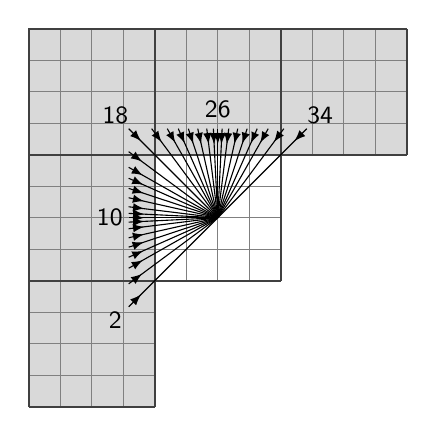
\begin{tikzpicture}[scale=1.60]

	\tikzset{middlearrow/.style={
		decoration={markings,
			mark= at position 0.95 with {\arrow{#1}} ,
		},
		postaction={decorate}
	}
}

	\def\startangle{45}
	\def\radius{0.707106781}

	\filldraw[fill=black!15, draw=black!75] (-6,-2) rectangle (-5,-1);
	\filldraw[fill=black!15, draw=black!75] (-6,-1) rectangle (-5,0);
	\filldraw[fill=black!15, draw=black!75] (-5,-1) rectangle (-4,0);
	\filldraw[fill=black!15, draw=black!75] (-6,-2) rectangle (-5,-3);
	\filldraw[fill=black!15, draw=black!75] (-4,0) rectangle (-3,-1);

	\draw[step=0.25,help lines] (-6,-2) grid (-4,0);
	\draw[step=0.25,help lines] (-6,-2) grid (-5,-3);
	\draw[step=0.25,help lines] (-4,0) grid (-3,-1);
	\draw[step=1,black!75,thick] (-6,-2) grid (-4,0);
	\draw[step=1,black!75,thick] (-6,-2) grid (-5,-3);
	\draw[step=1,black!75,thick] (-4,0) grid (-3,-1);

	% \foreach \direction in {2,3,...,34}
	\newcounter{direction}
	\setcounter{direction}{2}
    \foreach \position in {-32, -26, -21, -17, -13, -9, -5, -2, 0, 2, 5, 9,
	13, 17, 21, 26, 32, -26, -21, -17, -13, -9, -5, -2, 0, 2, 5, 9, 13, 17,
	21, 26, 32}
	{%
		% set the angle of current prediction direction 
		\pgfmathsetmacro{\angle}{\startangle - (\thedirection - 2) * 180 / 32 + 180}
        \ifthenelse{\thedirection < 19}
		{\pgfmathsetmacro{\angle}{-\position / 32 * 45 + 180}}
		{\pgfmathsetmacro{\angle}{-90 - \position / 32 * 45 + 180}}
		\ifthenelse{\thedirection < 18}{\def\oper{cos}}{\def\oper{sin}}
		\pgfmathsetmacro{\radnew}{abs(\radius / \oper(\angle))}
		\ifthenelse{\thedirection = 2 \OR \thedirection = 10 \OR \thedirection = 18 \OR \thedirection = 26 \OR \thedirection = 34}
		{\draw[opacity=0] (-4.5,-1.5) --++ (\angle:\radnew + 0.15) node
		[opacity=1] {\small \textsf{\thedirection}};}{}

		\draw[middlearrow={latex reversed}] (-4.5,-1.5) --++ (\angle:\radnew);

		% update direction for next iteration
		\stepcounter{direction}
	}
\end{tikzpicture}
}
	{\includegraphics{./figures/pred-scheme.pdf}}}
	\hspace{0.2\linewidth}
	\subfloat[Average intra prediction residual]
	{
\includegraphics[width=0.3\linewidth]{./figures/resids-scan-diag.png}}
	\caption[Example of \aclp{IPM} on a prediction residual]
	{Prediction scheme showing all \aclp{IPM} and a prediction
	residual example}
	\label{fig:pred_scheme}
\end{figure}

Intra prediction residuals present a correlation matrix that can be modelled
using a Toeplitz tridiagonal matrix, as the one
in~\eqref{eqn:tridiagonal_matrix}~\cite{han-10-spatial-adaptive-transform,
yueh-05-eigenvalues-tridiagonal}.
The eigenvalues of that correlation matrix can be expressed in a closed form
using the \ac{DST}-VII from~\eqref{eqn:dst_vii}.

\begin{equation}
	\tilde\R_x =
	\begin{pmatrix}
		1+\rho^2 & -\rho    & 0        & 0      & \hdots & 0            \\
		-\rho    & 1+\rho^2 & -\rho    & 0      & \hdots & 0            \\
		0        & -\rho    & 1+\rho^2 & -\rho  & \hdots & 0            \\
		0        & \ddots   & \ddots   & \ddots & \ddots & \vdots       \\
		\vdots   & \ddots   & \ddots   & \ddots & \ddots & -\rho        \\
		0        & \hdots   & 0        & 0      & -\rho  & 1+\rho^2-\rho
	\end{pmatrix}
	\label{eqn:tridiagonal_matrix}
\end{equation}
\index{tridiagonal matrix}

\begin{equation}
	{\left[S_{N}^{VII} \right]}_{n,k} =
	\frac{2}{\sqrt{2N+1}}\sin\left(\frac{\pi(2n-1)k}{2N+1}\right),
	\quad
	n,k = 1, \dots, N
	\label{eqn:dst_vii}
\end{equation}

Figure~\ref{fig:dct_dst}.b presents the \ac{DST}-VII bases for
$4\times4$ blocks.
The similarity between an average residual block from
figure~\ref{fig:pred_scheme}.b can be spotted by comparing it to the first
base vector from the \ac{DST}.

The use of the \ac{DST} in \ac{HEVC} over the \ac{DCT} on $4\times4$
blocks leads to a bit-rate reduction of 1\% on
average~\cite{sullivan-12-overview-hevc}.
An explanation on the adoption of the \ac{DST} into \ac{HEVC} is detailed in
Chapter~\ref{cha:mddt}, more precisely in \S\ref{sub:dst_and_mddt}.

\subsection{Final note on the \acs{KLT}}
\label{sub:final_note_on_the_klt}

The \ac{KLT} is often presented as the optimal transform, sometimes even for
all possible sources of signals.
However, it has been proved to be suboptimal in the transform coding / bit
allocation sense in some cases~\cite{effros-04-suboptimal-klt}.
For this reason, next section studies another kind of transform design that
leads to optimal transforms under different conditions.

\section{The rate-distortion optimised transform}
\label{sec:rdot}
\index{RDOT}

As discussed before, transforms try to find a compact representation of the
signal in the transform domain.
The \ac{KLT}, under certain assumptions, provides optimal bit allocation for
transformed coefficients and signal decorrelation.

Sezer proposes an alternative kind of transform to minimise the trade-off
between the distortion and the rate from~\eqref{eqn:lagrangian_rdo} by taking
into account the sparsity of the output signal in their
design~\cite{sezer-11-phd,sezer-08-sparse-orthonormal-transforms}.
This transform, named \ac{RDOT}, unlike the \ac{KLT}, does not make use
of the high-resolution assumption.
Instead, the bit-rate constraint is modelled via the sparsity of the
transformed coefficients, by the introduction of the $\ell_0$ norm, which
counts the number of non-zero coefficients in a vector.
The proposed \ac{RDOT} can be expressed as:
\begin{equation}
	\A_{opt} = \arg\min\limits_{\A}
	\sum_{\forall i} \min\limits_{\c_i}
	\left(
	{\Vert \x_i - \A^T\c_i \Vert}_2^2 + \lambda{\Vert \c_i \Vert}_0
	\right)
	\label{eqn:rdot-nsep}
\end{equation}
Where $\x_i$ are the input signals, i.e.\ a block of the training set,
$\c_i$ are its quantised transformed coefficients using the transform
$\A$.
$\A^T$ is its transposed matrix, as $\A$ is chosen orthogonal.
The constraint in the cost function is the $\ell_0$ norm of the coefficients,
i.e.\ the number of non-zero coefficients.
Finally, $\lambda$ is the Lagrange multiplier that tunes the constraint.

The fact that this transform design strives to obtain sparse signals in the
transform domain seems to be adapted to the state-of-the-art video coding
standard, \ac{HEVC}.
There are numerous syntax elements in \ac{HEVC} that deal with sparsity:
for a given transformed residual, the position of the last non-zero value is
signalled, meaning that, instead of explicitly transmitting all the following
zeroes, it is indicated that from that point onwards, all the values are zero.
More generally, flags indicating whether the individual coefficients are
significant or not are also part of the standard syntax.
Therefore, increasing the number of zeros of the quantised coefficients in the
transform domain seems a good objective.

A thorough study of~\eqref{eqn:rdot-nsep} analysing its properties and
consequences is detailed below.

\subsection{The \acs{RDOT} metric}
\label{sub:the_rdot_metric}
\index{RDOT metric}

The value that \ac{RDOT} minimises is expressed in~\eqref{eqn:rdot_metric} for
a single signal.
This metric depends exclusively on the quantisation step $\Delta$ and the
used transform $\A$.
It is shown in \S\ref{sub:the_lagrange_multiplier} that the Lagrange
multiplier $\lambda$ is tied to the quantisation step $\Delta$.
\begin{equation}
	J (\lambda) =
	{\Vert \x - \A^T \c \Vert}_2^2 + \lambda{\Vert \c \Vert}_0
	\label{eqn:rdot_metric}
\end{equation}
The first part of the equation represents the distortion introduced by
the quantisation.
The second term serves as a rate constraint, by ensuring that the number of
significant values in the transform domain is minimised together with the
distortion.

The minimisation of the metric is done in two steps, carried out iteratively
until convergence:
\begin{enumerate}
	\item Finding the optimal coefficients for a given transform.
	\item Updating the transform for the optimal coefficients.
\end{enumerate}

These two steps are detailed in the subsections below.
\subsubsection{Optimal coefficients for a given transform}
\label{ssub:optimal_coefficients_for_a_given_transform}

The optimal coefficients that introduce the minimum distortion for a given
quantisation step $\Delta$ are obtained by transforming the signal and
hard-thresholing them:
\begin{equation}
	\c = \lfloor \X \rfloor = \lfloor \A \x \rfloor
\end{equation}
The threshold value is tightly related to the Lagrange multiplier $\lambda$,
as demonstrated in \S\ref{sub:the_lagrange_multiplier}:
\begin{equation}
	\c[n] =
	\begin{cases}
		\X[n] & \vert \X[n] \vert \ge \displaystyle \frac{\Delta}{2} \\
		0     & \text{otherwise} \\
	\end{cases}
	\label{eqn:hard_threshold}
\end{equation}

\subsubsection{Optimal transform for given coefficients}
\label{ssub:optimal_transform_for_given_coefficients}

Once the optimal coefficients have been found, the transform $\A$, chosen
orthogonal, is updated to provide the mapping between $\x$ and $\c$ while
minimising the reconstruction error.
\begin{equation}
	\A_{opt} = \arg\min\limits_{\A}
	\left(
	\sum_{\forall i}{\Vert \x_i - \A^T\c_i\Vert}^2
	\right)
	\qquad \text{s.t. } \A\A^T = \I
\end{equation}
Since the expression is a scalar value, it can be rewritten using the trace
(the sum of a matrix diagonal):
\begin{equation}
	\A_{opt} = \arg\min\limits_{\A}
	\left(\sum_{\forall i}\tr\left( 
	{\left(\x_i - \A^T\c_i\right)}^T\left( \x_i - \A^T\c_i\right)
	\right)\right)
\end{equation}
Operating:
\begin{equation}
	\A_{opt} = \arg\min\limits_{\A}
	\left(\sum_{\forall i}\tr\left( 
	\x_i^T\x_i -\x_i^T\A^T\c_i -\c_i^T\A\x_i + \c_i^T\A\A^T\c_i
	\right)\right)
\end{equation}
Since the trace is a linear operator and $\A\A^T=\I$:
\begin{equation}
	\A_{opt} = \arg\min\limits_{\A}
	\left(\sum_{\forall i}
	\tr\left(\x_i^T\x_i\right)
	-\tr\left(\x_i^T\A^T\c_i\right)
	-\tr\left(\c_i^T\A\x_i\right)
	+\tr\left(\c_i^T\c_i \right)
	\right)
\end{equation}
Making use of the cyclic property of the trace and removing
$\A$-independent terms:
\begin{equation}
	\A_{opt} = \arg\min\limits_{\A}
	\left(\sum_{\forall i}
	-2\tr\left(\c_i\x_i^T\A^T\right)
	\right)
\end{equation}
Defining $\Y=\displaystyle\sum_{\forall i}\c_i\x_i^T$ and its \ac{SVD}
$\Y=\U\Lambdab^{\nicefrac{1}{2}}\V^T$, where $\U$ and $\V$
are orthogonal and $\Lambdab$ is a positive semi-definite diagonal matrix.
The equation rewrites as follows:
\begin{equation}
	\A_{opt} = \arg\min\limits_{\A}
	\left(
	-2\tr\left(\U\Lambdab^{\nicefrac{1}{2}}\V^T\A^T\right)
	\right)
\end{equation}
Minimising a negative expression is equivalent to maximising its positive
version, and re-arranging the terms using the trace cyclic property:
\begin{equation}
	\A_{opt} = \arg\max\limits_{\A}
	\left(
	2\tr\left(\Lambdab^{\nicefrac{1}{2}}\V^T\A^T\U\right)
	\right)
\end{equation}
Let $\Pb=\V^T\A^T\U$.
Since $\V$, $\A$ and $\U$ are orthogonal, so is $\Pb$.
The equation is now:
\begin{equation}
	\A_{opt} = \arg\max\limits_{\A}
	\left(
	\tr\left(\Lambdab^{\nicefrac{1}{2}}\Pb\right)
	\right)
\end{equation}
Since $\Lambdab$ is a diagonal matrix whose entries are non-negative by
definition and $\Pb$ is orthogonal, the maximisation is achieved when
$\Pb=\I$:
\begin{equation}
	\V^T\A_{opt}^T\U=\I\quad \Rightarrow \quad \A_{opt} = \U\V^T
\end{equation}

Summing up, the optimal transform is obtained using the \ac{SVD} of the
covariance matrix between the output signal (the transformed and quantised
coefficients) and the input signal (the prediction residuals).

\subsection{Separable \acs{RDOT} design}
\label{sub:separable_rdot_design}
\index{separable RDOT}
\index{RDOT}

The methods for transform design and learning presented in the previous
sections are non-separable.
This means that the input block is linearised and the transform is applied in
one single step.
Due to computational complexity issues, non-separable transforms are hardly
used in performing solutions.
A lower complexity approach involves separable transforms, which may not be
able to concentrate the energy in the transform domain as well as their
non-separable counterparts, as explained in \S\ref{sub:separability}.
In order to design and learn separable transforms, the design and learning
methods have to be adapted.
In the case of the \ac{KLT}, it is straightforward to see that one can learn a
horizontal \ac{KLT} to transform the rows of the signal and a vertical
\ac{KLT} for the columns.
However, the \ac{RDOT} algorithm needs further tuning in order to obtain
separable transforms.
A possible way of learning a separable \ac{RDOT} was also proposed by
Sezer~\cite{sezer-11-phd} and validated by independent
researches~\cite{sole-09-sparsity-optimisation-separable-transforms}.
The proposed method consists in updating each one of the horizontal and
vertical transforms separately, also chosen to be orthogonal transforms.

The separable transformation of a block $\x$ has been previously defined as a
two step transformation in~\eqref{eqn:sep_transform}:
\begin{equation*}
  \X = {\A_v\left( \A_h \x^T \right)}^T = \A_v \x \A_h^T
\end{equation*}

Where $\x$ is the two-dimensional block to transform, $\A_h$ is the horizontal
transform, used to transform the rows of $\x$ and $A_v$ is the vertical
transform, used to transform the resulting columns.

The equation to be optimised using separable transforms reads as follows:
\begin{equation}
	\A_{v_{opt}}, \A_{h_{opt}} = \arg\min\limits_{\A_v,\A_h}
	\left(
	\sum_{\forall i} \min\limits_{\c_i}{\Vert \x_i - \A_v^T\c_i\A_h \Vert}_2^2
	+ {\Vert \c_i \Vert}_0
	\right)
	\label{eqn:rdot-sep}
\end{equation}

This minimisation problem can be solved in a similar way to the non-separable
version.

\subsubsection{Optimal coefficients for a given transform}

As in the non-separable problem, the optimal coefficients $\c_i$ are found by
hard-thresholding the components of $\X_i=\A_v\x_i\A_h^T$ with
$\nicefrac{\Delta}{2}$.

\subsubsection{Optimal vertical transform for given coefficients}
The vertical transform needs to be updated accordingly:
\begin{equation}
	\A_{v_{opt}} = \text{arg}\min\limits_{\A_v}
	\left(
	\sum_{\forall i} {\Vert \x_i - \A_v^T\c_i\A_h \Vert}_2^2
	\right)
	\qquad \text{s.t. } \A_v\A_v^T = \I
\end{equation}
Expanding the expression and grouping the terms as in the non-separable
the covariance matrix $\Y$ can be defined as:
\begin{equation}
\Y = \sum_{\forall i} \c_i\A_h\x_i =
\U\Lambdab^{1/2}\V^T
\end{equation}
Then the optimal transform is given by:
\begin{equation}
  \A_{v_{opt}} = \U\V^T
\end{equation}

\subsubsection{Optimal coefficients for updated vertical transform}

As in the non-separable problem, the optimal coefficients $\c_i$ are
determined by hard-thresholding the components of $\X=\A_{v_{opt}}\x_i\A_h^T$
with $\nicefrac{\Delta}{2}$. However, this time the optimal vertical
transform from the previous step is used.

\subsubsection{Optimal horizontal transform for given coefficients}

Similarly, the horizontal transform needs to be updated accordingly:
\begin{equation}
	\A_{h_{opt}} = \text{arg}\min\limits_{\A_h}
	\left(
	\sum_{\forall i} {\Vert \x_i - \A_{v_{opt}}^T\c_i\A_h \Vert}_2^2
	\right)
	\qquad \text{s.t. } \A_h\A_h^T = \I
\end{equation}
Expanding the expression and grouping the terms as in the non-separable
the covariance matrix $\Y$ can be defined as:
\begin{equation}
	\Y = \sum_{\forall i} \c_i^T\A_{v_{opt}}\x_i =
\U\Lambdab^{1/2}\V^T
\end{equation}
The optimal transform is given by:
\begin{equation}
	\A_{h_{opt}} = \U\V^T
\end{equation}

Hence, the optimal transform are obtained in two iteratively alternated steps
until convergence.

\subsection{The Lagrange multiplier and the zero norm}
\label{sub:the_lagrange_multiplier}
\index{generalised normal distribution}
\index{generalised Gaussian distribution}
\index{exponential power distribution}
\index{Lagrange muliplier}
\index{zero norm}

Video coding residuals distribution can be modelled using a \ac{GGD}, also
known as generalised normal distribution or exponential power
distribution~\cite{lam-00-dct-coefficient-distribution,
yovanof-96-analysis-dct-coefficients}.
For this reason, in order to obtain the optimal Lagrange multiplier in a
reasonably general case, a \ac{GGD} is used to represent the residuals
\ac{PDF}.

Figure~\ref{fig:probability_density_functions} illustrates the \acp{PDF}
of a set of residuals transformed with the \ac{DCT} and the same residuals
transformed with an adapted \ac{RDOT}.  As expected, the \ac{RDOT},
represented by the red curve, presents higher sparsity than the generic
\ac{DCT}, in black:
its value is above the \ac{DCT} on zero, meaning that the coefficients have
more zeros when using the \ac{RDOT}.
Using different transforms, modifies the resulting \ac{PDF}, but since the
used transforms are orthogonal, the variance remains unaltered.
Additionally, since residuals are computed as the difference between predicted
and original blocks, they are prediction errors.
These errors are generated by excess or defect evenly, evidenced by their
zero-mean \ac{PDF}, which is symmetrical and centred around zero.
\begin{figure}[tb]
	\centering
	\ifthenelse{\usepdfs = 0}
	{\definecolor{greenish}{RGB}{0,145,0}
\begin{tikzpicture}[
	declare function={gamma(\z)=
    (2.506628274631*sqrt(1/\z) + 0.20888568*(1/\z)^(1.5) + 0.00870357*(1/\z)^(2.5) - (174.2106599*(1/\z)^(3.5))/25920 - (715.6423511*(1/\z)^(4.5))/1244160)*exp((-ln(1/\z)-1)*\z);},
	declare function={b(\s,\g)=
	1/\s*sqrt(gamma(3/\g)/gamma(1/\g));},
	declare function={a(\s,\g)=
	b(\s,\g)*\g/(2*gamma(1/\g));},
	declare function={ggd(\s,\g,\x)=
	a(\s,\g)*exp(-(abs(\x)*b(\s,\g))^\g);}
]
	\pgfplotsset{/tikz/font={\small}}
	\begin{axis}[
			xlabel={Values},
			ylabel={Density},
			grid=both,
			scale only axis,
			width=0.9\textwidth,
			height=0.30\textheight,
			scaled y ticks = false,
			% xtick={0,2,...,22},
			% x tick label style={
			% 	/pgf/number format/.cd,
			% 	set thousands separator={\thinspace},
			% 	/tikz/.cd
			% },
			% ytick={0,0.01,...,0.09},
			y tick label style={
				/pgf/number format/.cd,
				set decimal separator={.},
				fixed,
				fixed zerofill,
				precision=2,
				/tikz/.cd
			},
			xmin=-20, xmax=20,
			ymin=0, ymax=0.14,
			legend style={nodes=right},
			legend pos= north east,
			unbounded coords=jump,
		]

		\pgfplotstableread{figures/pdf_dct.dat}\table
		\addplot[black, thick, smooth, tension=0.3]
		table[x=x,y=dct,col sep=tab] from \table;
		\addlegendentry{DCT}

		\pgfplotstableread{figures/pdf_rdot.dat}\table
		\addplot[red, thick, smooth, tension=0.3]
		table[x=x,y=rdot,col sep=tab] from \table;
		\addlegendentry{RDOT}

		\addplot[blue, dotted, thick, samples=51, smooth, domain=-20:20]
		{ggd(5.1,1,x)};
		\addlegendentry{GGD($\sigma$,1,$x$)}

		\addplot[greenish, dashed, thick, samples=51, smooth, domain=-20:20]
		{ggd(5.1,2,x)};
		\addlegendentry{GGD($\sigma$,2,$x$)}
	\end{axis}
\end{tikzpicture}
}
	{\includegraphics{./figures/pdfs_plot.pdf}}
	\caption[Different residuals \acsp{PDF} compared to Laplace and Normal
	distributions]
	{\acsp{PDF} of the residuals with different transforms
	compared to Laplace and normal distributions}
	\label{fig:probability_density_functions}
\end{figure}
\index{probability density function}
\index{PDF}
Figure~\ref{fig:probability_density_functions} also includes the
\ac{PDF} of a Laplace distribution and a normal distribution.
Those two distributions are particular cases of a \ac{GGD}.

The centred \ac{GGD} \ac{PDF} can be expressed compactly as:
\index{gamma function}
\begin{equation}
	\GGD(\sigma,\gamma,x)=
	a\e^{-{\left(b\vert x \vert\right)}^\gamma}
	\label{eqn:ggd}
\end{equation}
Where:
\begin{align}
	b &= \frac{1}{\sigma}\sqrt{
	\frac{\Gamma\left(\nicefrac{3}{\gamma}\right)}
	{\Gamma \left(\nicefrac{1}{\gamma}\right)}} \\
	a &= \frac{b\gamma}{2\Gamma \left(\nicefrac{1}{\gamma}\right)}
\end{align}
and $\Gamma(z)$ is the gamma function, defined as:
\begin{equation}
	\Gamma(z) = \int_0^\infty t^{z-1}\e^{-t}\d t
\end{equation}
\index{Laplace distribution}
\index{Gaussian distribution}
\index{normal distribution}
\index{uniform distribution}
The Laplace and normal or Gaussian \acp{PDF} are achieved with
$\gamma=1$ and $\gamma=2$, respectively.
The uniform distribution can even be reached by making $\gamma\to\infty$.
However, from figure~\ref{fig:probability_density_functions} one could
approximate the video coding residuals \ac{PDF} with
$1\le\gamma\le2$~\cite{li-08-laplacian-modeling-dct-coefficients}.

In Sezer's work~\cite{sezer-11-phd,sezer-08-sparse-orthonormal-transforms},
the optimal value of the Lagrange multiplier $\lambda$ has been claimed
to be straightforward to obtain.
Nevertheless, no analytical way of proving its optimality has been found in
the literature.
Hence, a detailed study has been carried out below.

In order to find the optimal $\lambda$ from~\eqref{eqn:rdot_metric},
which describes the trade-off between the distortion and the rate,
$J(\lambda)$ has to be derived.
The problem will be tackled in two separate steps:
\begin{enumerate}
	\item Compute the distortion analytically and derive it.
	\item Compute the rate constraint and derive it.
\end{enumerate}
It has been decided to normalise the~\eqref{eqn:rdot_metric} by $N$ (the
signal dimension) so as to simplify the equations.
This scaling factor does not affect the solution.

\subsubsection{Derivation of the distortion function}
\label{ssub:derivation_of_the_distortion_function}

The distortion introduced by the hard-thresholding
from~\eqref{eqn:hard_threshold} can be expressed as:
\begin{equation}
	D
	= \frac{1}{N} \int_{-\infty}^{\infty} N {(x - \hat x)}^2 \P_X (x)\d x
	= \int_{\nicefrac{-\Delta}{2}}^{\nicefrac{\Delta}{2}}
	\label{eqn:int_distortion}
	x^2\P_X (x) \d x
\end{equation}
The integration intervals have been reduced to where the quantised values
differ from the original ones, that is, the values that have been affected by
the hard-thresholding from~\eqref{eqn:hard_threshold}.

Substituting $P_X(x)$ with the residuals \ac{PDF}:
\begin{align}
	D
	&=\int_{\nicefrac{-\Delta}{2}}^{\nicefrac{\Delta}{2}}
	x^2 a \e^{-{\left(b\vert x \vert\right)}^\gamma} \d x \\
	&=2 \int_0^{\nicefrac{\Delta}{2}}
	x^2 a \e^{-{\left(b x \right)}^\gamma} \d x\\
	&=
		2a \frac{\Gamma\left(\frac{3}{\gamma}\right)-
		\Gamma\left(
		\frac{3}{\gamma},{\left(\frac{b\Delta}{2}\right)}^\gamma
		\right)}{b^3\gamma}
	\label{eqn:distortion}
\end{align}
Where $\Gamma(a,z)$ is the incomplete upper gamma function, defined as:
\index{incomplete upper gamma function}
\begin{equation}
	\Gamma(a,z)=\int_z^\infty t^{a-1}\e^{-t}\d t
\end{equation}
Deriving~\eqref{eqn:distortion} in $\Delta$:
\begin{equation}
	\frac{\d D}{\d\Delta} =
	\frac{\Delta^2 a \e^{{(-b\nicefrac{\Delta}{2})}^\gamma}}{4}
	\label{eqn:diff_distortion}
\end{equation}

\subsubsection{Derivation of the zero norm function}
\label{ssub:derivation_of_the_zero_norm_function}

By definition, the $\ell_0$ norm is the total number of non-zero
elements in a vector.
Consequently, the constraint can be expressed as:
\begin{equation}
	R 
	= \frac{1}{N} N \P_X\left(\vert X \vert \ge \frac{\Delta}{2}\right)
	= 1-P_X\left(\vert X \vert < \frac{\Delta}{2}\right)
	= 1-\int_{\nicefrac{-\Delta}{2}}^{\nicefrac{\Delta}{2}}\P_X(x)\d x
	\label{eqn:int_rate}
\end{equation}
Substituting $P_X(x)$ with the residuals \ac{PDF}:
\begin{align}
	R
	&=1-\int_{\nicefrac{-\Delta}{2}}^{\nicefrac{\Delta}{2}}
	a \e^{-{\left(b\vert x \vert\right)}^\gamma} \d x \\
	&=1-2\int_0^{\nicefrac{\Delta}{2}}
	a \e^{-{\left(b x \right)}^\gamma} \d x \\
	&=1+2a\frac{\Gamma\left(
		\frac{1}{\gamma},{\left(\frac{b\Delta}{2}\right)}^\gamma\right)-
		\Gamma\left(\frac{1}{\gamma}\right)}
		{b\gamma}
	\label{eqn:rate}
\end{align}
Deriving~\eqref{eqn:rate} in $\Delta$:
\begin{equation}
	\frac{\d R}{\d\Delta} =
	-a\e^{{\left(\nicefrac{-b\Delta}{2}\right)}^\gamma}
	\label{eqn:diff_rate}
\end{equation}
\subsubsection{Optimal Lagrange multiplier}
\label{ssub:optimal_lagrange_multiplier}

With both the distortion~\eqref{eqn:diff_distortion} and the
constraint~\eqref{eqn:diff_rate} derived, the optimal Lagrange
multiplier can be found as:
\begin{equation}
	\frac{\d J(\lambda)}{\d \Delta}
	= \frac{\d D}{\d \Delta} +
	\lambda \frac{\d R}{\d \Delta} = 0 \\
	\label{eqn:diff_lagrange_multiplier}
\end{equation}
Substituting both derivatives:
\begin{equation}
	\frac{\Delta^2 a \e^{{(-b\nicefrac{\Delta}{2})}^\gamma}}{4}
	- \lambda
	a\e^{{\left(\nicefrac{-b\Delta}{2}\right)}^\gamma} = 0
	\quad \Rightarrow \quad \boxed{\lambda = \frac{\Delta^2}{4}}
\end{equation}

This proves how the Lagrange multiplier is only related to the quantisation
step.
In other words, once this value is fixed, so is the optimal balance between
the distortion and the rate constraint.

An important consequence of using the $\ell_0$ norm is that the optimal
Lagrange multiplier is independent from the data's \ac{PDF} (it does
not depend on $\sigma$ neither on $\gamma$), meaning that the optimal
Lagrange multiplier remains the same, no matter which transform has been
used.

In fact, these results can be generalised to any \ac{PDF}, making the
$\ell_0$ norm a robust approximation of the rate.
This property makes the $\ell_0$ norm suitable for iterative learning methods
where the transform changes at each iteration and so does the \ac{PDF} of the
training data in the transform domain.

\subsection{Independence from the \acs{PDF}}
\label{sub:independence_from_the_pdf}
\index{PDF}
\index{probablity density function}

In the previous subsection, for a given quantisation step, the value of
the optimal Lagrange multiplier $\lambda$ has been found for the particular
case of the residuals displaying \ac{PDF} that can be modelled after a
\ac{GGD}.
By using the fundamental theorem of calculus, which relates integrals
and derivatives of a function, one can generalise that conclusion for
any continuous \ac{PDF}.

Let $f(x)$ be the residuals \ac{PDF}.
The distortion is computed reusing~\eqref{eqn:int_distortion}:
\begin{equation}
	D = \int_{\nicefrac{-\Delta}{2}}^{\nicefrac{\Delta}{2}} x^2 f(x) \d x
\end{equation}
Deriving the distortion with respect to $\Delta$:
\begin{equation}
	\frac{\d D}{\d \Delta} =
	\frac{\Delta^2}{8}\left[
	f\left(\frac{\Delta}{2}\right)+f\left(-\frac{\Delta}{2}\right)\right]
\end{equation}
The rate constraint from~\eqref{eqn:int_rate} is computed as
follows with the generic \ac{PDF}
$f(x)$:
\begin{equation}
	R = 1 - \int_{\nicefrac{-\Delta}{2}}^{\nicefrac{\Delta}{2}} f(x) \d x\\
\end{equation}
Again, deriving with respect to $\Delta$:
\begin{equation}
	\frac{\d R}{\d \Delta} =
	-\frac{1}{2}\left[
	f\left(\frac{\Delta}{2}\right)+
	f\left(-\frac{\Delta}{2}\right)\right]
\end{equation}
Combining previous equations using~\eqref{eqn:diff_lagrange_multiplier},
is made clear that the optimal Lagrange multiplier $\lambda$ does not depend
on the residuals \ac{PDF}:
\begin{equation}
	\frac{\Delta^2}{8}\left[
	f\left(\frac{\Delta}{2}\right)+f\left(-\frac{\Delta}{2}\right)\right]
	- \lambda
	\frac{1}{2}\left[
	f\left(\frac{\Delta}{2}\right)+
	f\left(-\frac{\Delta}{2}\right)\right] = 0
\end{equation}
\begin{equation}
	\boxed{\lambda = \frac{\Delta^2}{4}}
\end{equation}

This fact makes the $\ell_0$ norm suitable even for distributions that cannot
be modelled after a \ac{GGD}.
The independence from the \ac{PDF} comforts the choice of the $\ell_0$
norm over other models that might provide a more realistic and accurate
approximation of the rate, such as the entropy.

An example of the $\ell_0$ norm independence from the \ac{PDF} is provided
below.
Consider the following scenario: some residuals \acp{PDF} that follow \ac{GGD}
with different exponents $\gamma$.
Consider, as well, a quantisation step $\Delta=14.256$, issued from a \ac{QP}
27 in \ac{HEVC}.
It has been demonstrated previously, that $J(\lambda)$
from~\eqref{eqn:rdot_metric} achieves its minimum value at
$\lambda=\frac{\Delta^2}{4}\approx50.81$, independently from the
residuals \ac{PDF} when modelling the rate with the $\ell_0$ norm.

However, if instead of using the $\ell_0$ norm, entropy (H) is used, it can no
longer be assumed that the optimal value of $\lambda$ providing the best
trade-off between distortion and rate does not depend on the residuals
\ac{PDF}.
Due to the complexity of the calculations involved then using the
entropy together with a uniform quantiser, the dependence to the
\ac{PDF} will be evidenced through the example from
figure~\ref{fig:j_lambda_qp}.
It shows that the value $J(\lambda)$ is plotted for various \acp{GGD} at
different \ac{QP} values, which served as the hard-threshold value.
When using the $\ell_0$ norm, $J(\lambda)$ reaches its minimum value at
QP 27, as expected.
On the other hand, using the entropy leads to a minimum value of
$J(\lambda)$ that is \ac{PDF}-dependent.
An unwanted consequence of this dependence is that, for an iterative
learning algorithm, after updating the transform at each iteration, the
new \ac{PDF} would have to be estimated to find the new optimal Lagrange
multiplier $\lambda$, thus complicating the whole learning process and
leading to probable instabilities.
\begin{figure}[tp]
	\centering
	\ifthenelse{\usepdfs = 0}
	{\definecolor{greenish}{RGB}{0,145,0}
\begin{tikzpicture}
	\pgfplotsset{/tikz/font={\small}}
	\begin{axis}[
			xlabel={quantisation parameter (QP)},
			ylabel={$J(\lambda)$},
			grid=both,
			scale only axis,
			width=0.9\textwidth,
			height=0.3\textheight,
			scaled y ticks = false,
			% x tick label style={
			% 	/pgf/number format/.cd,
			% 	set thousands separator={\thinspace},
			% 	set decimal separator={.},
			% 	fixed,
			% 	fixed zerofill,
			% 	precision=2,
			% 	/tikz/.cd
			% },
			% y tick label style={
			% 	/pgf/number format/.cd,
			% 	set decimal separator={.},
			% 	fixed,
			% 	fixed zerofill,
			% 	precision=1,
			% 	/tikz/.cd
			% },
			% xtick={0.20,0.22,...,0.50},
			% ytick={0,2.5,...,100},
			xmin=20, xmax=50,
			ymin=20, ymax=140,
			legend style={nodes=right},
			legend pos= south east,
			unbounded coords=jump,
		]
		\pgfplotstableread{figures/j_qp27.dat}\table
		\addplot[dashed, mark=*,mark size=1pt, greenish, thick, smooth, tension=0.3]
		table[x=qp,y=jh150,col sep=tab] from \table;
		\addlegendentry{$\gamma=1.50$ with H}

		\pgfplotstableread{figures/j_qp27.dat}\table
		\addplot[dashed, mark=*,mark size=1pt, blue, thick, smooth, tension=0.3]
		table[x=qp,y=jh125,col sep=tab] from \table;
		\addlegendentry{$\gamma=1.25$ with H}

		\pgfplotstableread{figures/j_qp27.dat}\table
		\addplot[dashed, mark=*,mark size=1pt, red, thick, smooth, tension=0.3]
		table[x=qp,y=jh100,col sep=tab] from \table;
		\addlegendentry{$\gamma=1.00$ with H}

		\pgfplotstableread{figures/j_qp27.dat}\table
		\addplot[dashed, mark=*,mark size=1pt, black, thick, smooth, tension=0.3]
		table[x=qp,y=jh075,col sep=tab] from \table;
		\addlegendentry{$\gamma=0.75$ with H}


		\pgfplotstableread{figures/j_qp27.dat}\table
		\addplot[mark=*,mark size=1pt, greenish, thick, smooth, tension=0.3]
		table[x=qp,y=jnz150,col sep=tab] from \table;
		\addlegendentry{$\gamma=1.50$ with $\ell_0$}

		\pgfplotstableread{figures/j_qp27.dat}\table
		\addplot[mark=*,mark size=1pt, blue, thick, smooth, tension=0.3]
		table[x=qp,y=jnz125,col sep=tab] from \table;
		\addlegendentry{$\gamma=1.25$ with $\ell_0$}

		\pgfplotstableread{figures/j_qp27.dat}\table
		\addplot[mark=*,mark size=1pt, red, thick, smooth, tension=0.3]
		table[x=qp,y=jnz100,col sep=tab] from \table;
		\addlegendentry{$\gamma=1.00$ with $\ell_0$}

		\pgfplotstableread{figures/j_qp27.dat}\table
		\addplot[mark=*,mark size=1pt, black, thick, smooth, tension=0.3]
		table[x=qp,y=jnz075,col sep=tab] from \table;
		\addlegendentry{$\gamma=0.75$ with $\ell_0$}

		\addplot [only marks, mark=o, mark size=3pt, thick] table {
		31	91.35
		32	87.31
		32	81.57
		33	73.01
		27	30.44
		27	28.89
		27	26.70
		27	23.45
		};
		\addlegendentry{$J(\lambda)_{\text{min}}$}

	\end{axis}

\end{tikzpicture}
}
	{\includegraphics{./figures/j_qp27_plot.pdf}}
	\caption
	[$J(\lambda)$ for different \acsp{GGD} modelling the rate with
	the $\ell_0$ norm and the entropy]
	{$J(\lambda)$ for different \acsp{GGD} modelling the rate with
	the $\ell_0$ norm and the entropy (H)}
	\label{fig:j_lambda_qp}
\end{figure}

\subsection{Rate-distortion improvement through the learning}
\label{sub:rate_distortion_improvement_through_the_learning}

Assuming the source \ac{PDF} can be modelled after a \ac{GGD} with a
given variance $\sigma^2$ and exponent $\gamma$, the impact of the
learning in terms of the $J(\lambda)$ from~\eqref{eqn:rdot_metric} can
be illustrated with the following example.
By learning an adapted transform over a set of residuals, the amount of
transformed coefficients mapped to zero increases, increasing its
kurtosis (the distribution ``looks more sharp''), hence reducing the
exponent $\gamma$.
Figure~\ref{fig:lambda_zero_norm_dist} illustrates the relationship
between the distortion and the rate model, at different \acp{QP}.
\acp{QP} 27 and 32 are highlighted, corresponding to quantisation steps
$\Delta = 14.256$ and $\Delta = 25.504$ in \ac{HEVC}, respectively.

\begin{figure}[tp]
	\centering
	\ifthenelse{\usepdfs = 0}
	{\definecolor{mygreen}{RGB}{0,143,0}
\begin{tikzpicture}
	\pgfplotsset{/tikz/font={\small}}
	\begin{axis}[
			xlabel={$\ell_0$ norm},
			ylabel={Distortion},
			grid=both,
			scale only axis,
			width=0.80\textwidth,
			height=0.30\textheight,
			scaled y ticks = false,
			x tick label style={
				/pgf/number format/.cd,
				set thousands separator={\thinspace},
				set decimal separator={.},
				fixed,
				fixed zerofill,
				precision=2,
				/tikz/.cd
			},
			y tick label style={
				/pgf/number format/.cd,
				set decimal separator={.},
				fixed,
				fixed zerofill,
				precision=1,
				/tikz/.cd
			},
			% xtick={0.20,0.22,...,0.50},
			% ytick={0,2.5,...,100},
			xmin=0.00, xmax=0.70,
			ymin=0.00, ymax=100,
			legend style={nodes=right},
			legend pos= north east,
			unbounded coords=jump,
		]

		\pgfplotstableread{figures/dist_zero_qp.dat}\table
		\addplot[mark=*,mark size=1pt, mygreen, thick, smooth, tension=0.3]
		table[x=nz150,y=d150,col sep=tab] from \table;
		\addlegendentry{$\gamma=1.50$}

		\pgfplotstableread{figures/dist_zero_qp.dat}\table
		\addplot[mark=*,mark size=1pt, blue, thick, smooth, tension=0.3]
		table[x=nz125,y=d125,col sep=tab] from \table;
		\addlegendentry{$\gamma=1.25$}

		\pgfplotstableread{figures/dist_zero_qp.dat}\table
		\addplot[mark=*,mark size=1pt, red, thick, smooth, tension=0.3]
		table[x=nz100,y=d100,col sep=tab] from \table;
		\addlegendentry{$\gamma=1.00$}

		\pgfplotstableread{figures/dist_zero_qp.dat}\table
		\addplot[mark=*,mark size=1pt, black, thick, smooth, tension=0.3]
		table[x=nz075,y=d075,col sep=tab] from \table;
		\addlegendentry{$\gamma=0.75$}

		\addplot [only marks, mark=o, mark size=3pt, thick] table {
		% QP 27
		0.434317	8.396036
		0.404402	8.363620
		0.364981	8.176391
		0.310958	7.666366
		};
		\addlegendentry{$\lambda_{opt}$ QP 27}

		\addplot [only marks, mark=o, mark size=3pt, thick, dashed] table {
		0.144763	23.171433
		0.164659	27.008339
		0.178336	29.754038
		0.188380	31.800229
		};
		\addlegendentry{$\lambda_{opt}$ QP 32}

	\end{axis}

\end{tikzpicture}
}
	{\includegraphics{./figures/dist_zero_qp_plot.pdf}}
	\caption{Distortion and $\ell_0$ norm with $\lambda_{opt}$ at
	\acsp{QP} 27 and 32 for different \acsp{PDF}}
	\label{fig:lambda_zero_norm_dist}
\end{figure}

As the exponent $\gamma$ decreases, so do both terms of $J(\lambda)$,
the distortion and the $\ell_0$ norm.
It can also be seen that since the Lagrange multiplier value $\lambda$
does not change, neither does the slope of a tangent line to the circled
points, corresponding to the optimal trade-off between the distortion
and the rate constraint.
The amount of improvement in each direction is weighted by $\lambda$: at
\ac{QP} 27 there is more room for sparsity improvement than there is for
reducing the distortion, compared to \ac{QP} 32.

\section{Conclusions}
\label{sec:conclusions_transforms}

This chapter has introduced different types of transforms and some
basic concepts, such as separability and its relation to computational
complexity.

Two different approaches of transform design have been studied:
the \ac{KLT} and the \ac{RDOT}.
The \ac{KLT} defines the transform providing optimal bit allocation under the
high-resolution hypothesis.
The \ac{DCT} and \ac{DST} used in \ac{HEVC} have been obtained from the
\ac{KLT} for particular kinds of signals.

The \ac{RDOT} finds the optimal balance between the distortion introduced by
the quantiser and a rate constraint, expressed in terms of signal sparseness.
A detailed study on its design, based on the $\ell_0$ norm, has been carried
out to justify the appropriateness of the approach, lacking in current
literature.

In the next chapter, both transform designs will be tested in a real
scenario to evaluate their performances in video coding.


\chapter{The mode-dependent directional transforms}
\label{cha:mddt}
\chaptertoc

\section{Introduction}
\label{sec:mddt_introduction}

The previous Chapter has introduced two different transform design approaches.
In order to test their performances for video coding, a technique called
\ac{MDDT} is developed in this section.
The principle of the \ac{MDDT} lies on using an adapted transform learnt
specifically for each \acf{IPM}.

The \ac{MDDT} technique was proposed during the \ac{HEVC} standardisation
phase, but is was finally discarded in favour of a new transform, the
\ac{DST} as explained in \S\ref{sub:dst_and_mddt}.

\subsection{Motivation and principles of the \acs{MDDT}}
\label{sub:mddt_motivation}
\index{MDDT}

Depending on the selected prediction mode, transformed coefficients might
present different patterns, making low and high values appear at different
block positions.
This heterogeneity can be harmful for the entropy coding, which is one of the
reasons why different scanning patterns exist in
\ac{HEVC}~\cite{sole-12-transform-coefficient-coding}.
These scanning patterns, presented in the lower part of
figure~\ref{fig:mdcs} depend only on the \ac{IPM} used to compute the
residual.

The \ac{MDDT} was motivated by the fact that residuals issued from different
\acp{IPM} present notable differences.
An example of these differences is presented in
figure~\ref{fig:residual_differences} for $4\times4$ and $8\times8$ prediction
residuals.
An adapted transform for each \ac{IPM} can provide good signal compaction by
specialisation, which means having an adapted transform for each one of the 35
\acp{IPM}.

\begin{figure}[tb]
	\centering
	\subfloat[$4\times4$ --- \acs{IPM} 6]
	{
\includegraphics[width=0.2\linewidth]{./figures/avg-residual-s4-p06.png}}
	\hfill
	\subfloat[$4\times4$ --- \acs{IPM} 10]
	{
\includegraphics[width=0.2\linewidth]{./figures/avg-residual-s4-p10.png}}
	\hfill
	\subfloat[$4\times4$ --- \acs{IPM} 18]
	{
\includegraphics[width=0.2\linewidth]{./figures/avg-residual-s4-p18.png}}
	\hfill
	\subfloat[$4\times4$ --- \acs{IPM} 26]
	{
\includegraphics[width=0.2\linewidth]{./figures/avg-residual-s4-p26.png}}
	\\
	\subfloat[$8\times8$ --- \acs{IPM} 6]
	{
\includegraphics[width=0.2\linewidth]{./figures/avg-residual-s8-p06.png}}
	\hfill
	\subfloat[$8\times8$ --- \acs{IPM} 10]
	{
\includegraphics[width=0.2\linewidth]{./figures/avg-residual-s8-p10.png}}
	\hfill
	\subfloat[$8\times8$ --- \acs{IPM} 18]
	{
\includegraphics[width=0.2\linewidth]{./figures/avg-residual-s8-p18.png}}
	\hfill
	\subfloat[$8\times8$ --- \acs{IPM} 26]
	{
\includegraphics[width=0.2\linewidth]{./figures/avg-residual-s8-p26.png}}
	\caption{Average residual profiles for different \acsp{IPM}}
	\label{fig:residual_differences}
\end{figure}

A possible implementation of the \ac{MDDT} inside a video coding scheme is
illustrated in figure~\ref{fig:mddt_enc}.
This encoder works in the same way as the hybrid encoder from
figure~\ref{fig:hybrid_video_coding_scheme}, with the exception that, in this
case, each \ac{IPM} will be tested in the \ac{RDO} loop with its corresponding
transform.
Three examples of residuals are shown:
for \acp{IPM} 10, 18 and 26, which are obtained as the differences between the
predictions derived from their corresponding \acp{IPM} and the original image.
The \ac{IPM} 10 stands for a horizontal prediction from left blocks, 18 for
the diagonal, from upper and left blocks and 26 for the vertical prediction
from the upper blocks.
When inside the \ac{RDO} loop, each intra prediction residual is tested using
the assigned transform.
Then, the \ac{IPM} offering the best rate-distortion trade-off is selected and
signalled into the bitstream.

On the decoder side (figure~\ref{fig:mddt_dec}), the only needed information
to decode the block is represented in coloured blocks:
the transformed coefficients and the used \ac{IPM}.
No additional information has to be sent to the decoder, with regards to the
hybrid video coding scheme:
the signalled \ac{IPM} allows the decoder to know which transform to use to
convert the transformed coefficients back to the pixel domain, without having
to perform any extra calculations or take any decisions.

One of the positive aspects of the \ac{MDDT} is the fact that, despite having
more than one transform for a particular block size, only the transform
corresponding to the selected \ac{IPM} is used to transform that residual.
This means that, the \ac{IPM} conditions the transform, so there is no extra
step in the \ac{RDO} loop for the transform.
However, there might be an increase of the complexity on both \ac{MDDT}
encoder and decoder due not to the number of transforms, but to the possible
lack of fast algorithms for the adapted transforms implementation.

\begin{figure}[tp]
	\centering
	\ifthenelse{\usepdfs = 0}
	{% \documentclass{book}
% \usepackage{tikz, libertine}
% \begin{document}

\pgfmathsetmacro{\nodebasesize}{1} % A node with a value of one will have this diameter
\pgfmathsetmacro{\nodeinnersep}{0.1}

\tikzstyle{bloq} = [rectangle, draw, text badly centered, minimum height=2.5em, inner sep=1mm]

\tikzstyle{frame} =
[rectangle, fill=white, draw, text badly centered, minimum width=3*\h em,minimum height=3*\v em]

\tikzset{
	middlearrow/.style={
		decoration={markings,
		mark= at position 0.9 with {\arrow{#1}},
		},
		postaction={decorate}
	}
}

\newcommand{\bloq}[4]{% position, name options, label
	\node[bloq,#3] (#2) at (#1) {\textsf{#4}};
}
\newcommand{\add}[2]{%position, name
	\draw (4,4) circle [radius=0.3] node (add) {\textsf$+$};
}

\newcommand{\propnode}[5]{% position, name, options, value, label
	\pgfmathsetmacro{\minimalwidth}{sqrt (#4*\nodebasesize)}
	\node[#3,minimum width=\minimalwidth*1cm,inner sep=\nodeinnersep*0cm,circle,draw]
	(#2) at (#1) {#5};
}


\begin{tikzpicture}[scale=1.5,x=1em,y=1em]
\tikzstyle{every node}=[font=\small]
	\def\x{0}
	\def\y{0}
	\def\thickness{thick}
	\def\h{2.0}
	\def\v{1.0}

% INPUT VIDEO SEQUENCE
	\draw (\x-\h,\y+0.5*\v) node[above] {\textsf{Input Video Sequence}};
	\draw (\x-\h,\y-3*\v) node[above] {\textsf{Split into blocks}};
	\node[frame] at (\x-\h-0.3,\y-\v+0.3){};
	\node[frame] at (\x-\h-0.2,\y-\v+0.2){};
	\node[frame] at (\x-\h-0.1,\y-\v+0.1){};
	\node[frame] (sequence) at (\x-\h,\y-\v){};
	\draw[step=0.25,thin,help lines] (\x,\y) grid (-2*\h,-2*\v);
	\draw[step=0.5,thin] (\x,\y) grid (-2*\h,-2*\v);
	\draw[step=1.0,black,thick] (\x,\y) grid (-2*\h,-2*\v);

	\propnode{\x+1*\h,\y-1*\v}{add1}{fill=green!50}{0}{$+$}
	\propnode{\x+8*\h,\y-9*\v}{add2}{fill=green!50}{0}{$+$}
	\propnode{\x+0.75*\h/2,\y-1*\v}{inter1}{fill=black}{0.005}{}
	\propnode{2,\y-9*\v}{inter2}{fill=black}{0.005}{}

	\draw (\x+1.25*\h,\y-0.75*\v) node[above] {\textsf{residuals}};

	\bloq{\x+3*\h,\y-\v}{Transf}{text width=6em,fill=red!50}
	{$\cdots$\\[-0.25em]
	Transf. 10\\[-0.25em]
	$\cdots$\\[-0.25em]
	Transf. 18\\[-0.25em]
	$\cdots$\\[-0.25em]
	Transf. 26\\[-0.25em]
	$\cdots$\\[-1.5em]};
	\bloq{\x+6*\h,\y-\v}{Quant}{text width=6em,fill=yellow!50}{Quant.};
	\bloq{\x+8*\h,-\y-4*\v}{InvQuant}{text width=6em,fill=yellow!50}{Inv. Quant.};
	\bloq{\x+8*\h,\y-7*\v}{InvTransf}{text width=6em,fill=red!50}{Inv. Transf. $k$};
	\bloq{\x+8*\h,\y-12.5*\v}{Reconst}{text width=4em,fill=black!15}{Reconst.\\block};
	\bloq{\x+4.75*\h,\y-12.5*\v}{IntraPred}{text width=5em,text height=5em,fill=yellow!50}{};

	\draw[-latex,\thickness] (sequence) -- (add1) node [below right] {\textsf{$-$}};
	\draw[-latex,\thickness] (add1) -- (Transf);
	\draw[-latex,\thickness] (Transf) -- (Quant);
	\draw[-latex,\thickness] (Quant) -| (InvQuant);
	\draw[-latex,\thickness] (InvQuant) -- (InvTransf);
	\draw[-latex,\thickness] (InvTransf) -- (add2);
	\draw[-latex,\thickness] (add2) -- (Reconst);
	\draw[-latex,\thickness] (inter2) -- (add2);
	\draw[-latex,\thickness] (Reconst) -- (IntraPred);
	\draw[-latex,\thickness] (IntraPred) -| (add1);

	\def\startangle{45}
	\def\radius{0.707}
	\def\posx{\x+4*\h}
	\def\posy{\y-13*\v}

	\draw (\posx-3,\posy+1.5) node [below] {\small\textsf{Intra Prediction}};

	\tikzstyle{frame} =
	[rectangle, fill=white, draw, text centered, minimum width=4em, minimum height=2em]

	\filldraw[fill=black!15, draw=black!75] (\posx,\posy) rectangle (\posx+1,\posy+1);
	\filldraw[fill=black!15, draw=black!75] (\posx,\posy+1) rectangle (\posx+1,\posy+2);
	\filldraw[fill=black!15, draw=black!75] (\posx+1,\posy+1) rectangle (\posx+2,\posy+2);
	\filldraw[fill=white, draw=black!75] (\posx+1,\posy+1) rectangle (\posx+2,\posy);
	\filldraw[fill=black!15, draw=black!75] (\posx,\posy) rectangle (\posx+1,\posy-1);
	\filldraw[fill=black!15, draw=black!75] (\posx+2,\posy+2) rectangle (\posx+3,\posy+1);

	\draw[step=0.25,help lines] (\posx,\posy) grid (\posx+2,\posy+2);
	\draw[step=0.25,help lines] (\posx,\posy) grid (\posx+1,\posy-1);
	\draw[step=0.25,help lines] (\posx+2,\posy+2) grid (\posx+3,\posy+1);
	\draw[step=1,black!75,thick] (\posx,\posy) grid (\posx+2,\posy+2);
	\draw[step=1,black!75,thick] (\posx,\posy) grid (\posx+1,\posy-1);
	\draw[step=1,black!75,thick] (\posx+2,\posy+2) grid (\posx+3,\posy+1);

	\foreach \direction in {10,18,...,26}
	{%
		% set the angle of current prediction direction 
		\pgfmathsetmacro{\angle}{\startangle - (\direction - 2) * 180 / 32 + 180}
		\ifthenelse{\direction < 18}{\def\oper{cos}}{\def\oper{sin}}
		\pgfmathsetmacro{\radnew}{abs(\radius / \oper(\angle))}
		\ifthenelse{\direction=2 \OR \direction=10 \OR \direction=18 \OR \direction=26 \OR \direction=34}
		{
			\draw[opacity=0] (\posx+1.5,\posy+0.5) --++ (\angle:\radnew
			+ 0.25) node [opacity=1] {\small\textsf{\direction}};
		}{}
		\draw[middlearrow={latex reversed},very thin] (\posx+1.5,\posy+0.5) --++ (\angle:\radnew);
	}
	\draw(0.2,3) node
	{
\includegraphics[width=3em]{./figures/resids-scan-vert}\small\textsf{10}};
	\draw(3.2,3) node
	{
\includegraphics[width=3em]{./figures/resids-scan-diag}\small\textsf{18}};
	\draw(6.2,3) node
	{
\includegraphics[width=3em]{./figures/resids-scan-horz}\small\textsf{26}};
	\draw[thick,round cap-<](2.71,0) --++ (0,1.5);
	\draw[thick,round cap-round cap] (-1,2) ++ ( 255 : 0 ) arc ( 255:285:15 );
\end{tikzpicture}
% \end{document}
}
	{\includegraphics{./figures/mddt_enc.pdf}}
	\caption{Encoding scheme for the \acs{MDDT}}
	\label{fig:mddt_enc}
\end{figure}

\begin{figure}[tp]
	\centering
	\ifthenelse{\usepdfs = 0}
	{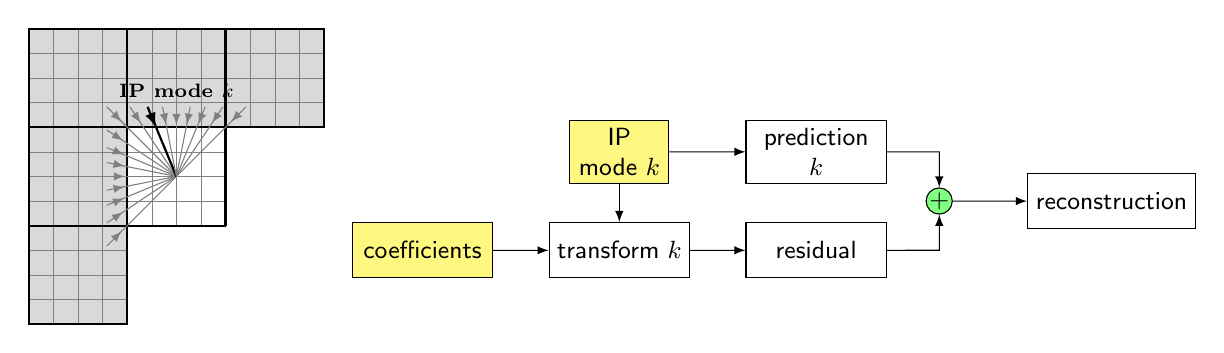
\begin{tikzpicture}[scale=1.25]
\tikzstyle{every node}=[font=\small]
	\tikzset{middlearrow/.style={
		decoration={markings,
			mark= at position 0.9 with {\arrow{#1}} ,
		},
		postaction={decorate}
	}
}

	\def\startx{0}
	\def\starty{0}
	\def\radius{3.0}
	\def\startangle{45}
	\def\colour{black}
	\def\thickness{help lines}
	\def\hdist{2}
	\def\startangle{45}
	\def\radius{0.707}
	\def\thickness{black!50}
	\def\selmode{ }
	\pgfmathsetmacro{\nodebasesize}{1} % A node with a value of one will have this diameter
	\pgfmathsetmacro{\nodeinnersep}{0.1}
	\tikzstyle{bloq} = [rectangle, draw, text badly centered, minimum height=2em, inner sep=1mm]
	\newcommand{\bloq}[4]{% position, name options,
		label \node[bloq,#3](#2) at (#1) {\textsf{#4}};
	}
	\newcommand{\propnode}[5]{% position, name, options, value, label
		\pgfmathsetmacro{\minimalwidth}{sqrt(#4*\nodebasesize)}
		\node[#3,minimum width=\minimalwidth*1cm,inner sep=\nodeinnersep*0cm,circle,draw] 
		(#2) at (#1) {#5};
	}

	\tikzstyle{frame} =
	[rectangle, fill=white, draw, text centered, minimum width=4em, minimum height=2em]

	\filldraw[fill=black!15, draw=black] (-6,-2) rectangle (-5,-1);
	\filldraw[fill=black!15, draw=black] (-6,-1) rectangle (-5,0);
	\filldraw[fill=black!15, draw=black] (-5,-1) rectangle (-4,0);
	\filldraw[fill=black!15, draw=black] (-6,-2) rectangle (-5,-3);
	\filldraw[fill=black!15, draw=black] (-4,0) rectangle (-3,-1);

	\draw[step=0.25,help lines] (-6,-2) grid (-4,0);
	\draw[step=0.25,help lines] (-6,-2) grid (-5,-3);
	\draw[step=0.25,help lines] (-4,0) grid (-3,-1);
	\draw[step=1,black,thick] (-6,-2) grid (-4,0);
	\draw[step=1,black,thick] (-6,-2) grid (-5,-3);
	\draw[step=1,black,thick] (-4,0) grid (-3,-1);

	\foreach \direction in {2,4,...,34}
	{%
		% set the angle of current prediction direction 
		\pgfmathsetmacro{\angle}{\startangle - (\direction - 2) * 180 / 32 + 180}
		\ifthenelse{\direction < 18}{\def\oper{cos}}{\def\oper{sin}}
		\pgfmathsetmacro{\radnew}{abs(\radius / \oper(\angle))}
		% draw the prediction direction lines with the appropriate colour
		\ifthenelse{\direction = 22}{\def\thickness{thick}\def\selmode{$k$}};
		\draw[\colour, \thickness, middlearrow={latex reversed}] (-4.5,-1.5) --++ (\angle:\radnew);
	}

	\draw(-4.5,-0.80) node[above] {\scriptsize \bf IP mode $k$};

	%\draw[-latex] (-2,-1.5) to [in=180,out= 00] ++ (1.30,0.25);
	%\draw[-latex] (-2,-1.5) to [in=180,out= 00] ++ (1.30,-0.75);

	%\draw (-4.5,-3.05) node[below] {\scriptsize Block to predict and decode};


	\draw[dotted](\startx,\starty -0.5) ++ (0,-2);

	\bloq{\startx,\starty-1.25}{ipk}{text width=3em,fill=yellow!50}{IP mode $k$}
	\bloq{\startx-\hdist,\starty-2.25}{coefk}{text width=4.5em,fill=yellow!50}{coefficients}

	\bloq{\startx+\hdist,\starty-1.25}{predk}{text width=4.5em}{prediction $k$}
	\bloq{\startx,\starty-2.25}{trk}{text width=4.5em}{transform $k$}

	\bloq{\startx+\hdist,\starty-2.25}{res}{text width=4.5em}{residual}

	\bloq{\startx+2.5*\hdist,\starty-1.75}{rec}{text width=5.5em}{reconstruction}

	\draw[-latex] (ipk) -- (predk);
	
	\draw[-latex] (ipk) -- (trk);

	\draw[-latex] (coefk) -- (trk);

	\draw[-latex] (trk) -- (res);

	\propnode{3.25,-1.75}{add1}{fill=green!50}{0}{\small+}

	\draw[-latex] (predk) --++ (1,0) -| (add1);
	\draw[-latex] (res) --++ (1,0) -| (add1);
	\draw[-latex] (add1) -- (rec);

\end{tikzpicture}

% vim:set filetype=tex:
}
	{\includegraphics{./figures/mddt_dec.pdf}}
	\caption{Decoding scheme for the \acs{MDDT}}
	\label{fig:mddt_dec}
\end{figure}

\subsection{The \acs{DST} as a simplification of the \acs{MDDT}}
\label{sub:dst_and_mddt}
\index{DST}
\index{KTA}
\index{TMuC}
\index{MDDT}
\index{HEVC}
\index{KLT}

The \ac{DST} has been presented as the \ac{KLT} for intra prediction residuals
in \S\ref{sub:particular_case_dct}.
The way of generating the prediction residuals leads to a particular kind of
signals with properties that differ from those of natural images.
As a result, the \ac{DCT} is no longer a good approximation of the \ac{KLT}.
However, it was not straightforward to realise that the \ac{KLT} for those
signals is the \ac{DST}:
many studies, detailed below, were carried out in order to find better
performing transform for these signals.

Over the \ac{HEVC} standardisation phase, various techniques to improve the
performance of \ac{AVC} were explored and designated as \ac{KTA}.
Amongst those techniques, in order to improve the coding performance of intra
prediction residuals, an adapted transform for each \ac{IPM} (at that time 9,
which evolved into 35 in \ac{HEVC}), was included in the \ac{KTA} software.
The adapted transforms were \acp{KLT}, and the resulting technique was called
\ac{MDDT}.
It became a core component of the \ac{TMuC}~\cite{JCTVC-A204} due to its
performance improvements over the previous standard.

During the \ac{JCT-VC} meetings, many efforts were done to yield the first
implementation of the \ac{MDDT}, which was non-separable, more
lightweight~\cite{VCEG-AG11}.

One of the first attempts was to make the \acp{KLT}
separable~\cite{JCTVC-B024}.
A fast algorithm was derived for the $4\times4$ transform by analysing
the correlation matrix of the intra prediction residuals, which can be
modelled using tridiagonal
matrices~\cite{yueh-05-eigenvalues-tridiagonal}.
In order to further reduce the complexity, rotational transforms were
also considered in~\cite{JCTVC-C096}.
The main idea was to use the \ac{DCT} followed by a secondary transform
implemented in the form of Given's
rotations~\cite{yang-04-matrix-decomposition} to improve the coding
efficiency.

The \ac{DST} was theoretically proved to be the optimal transform, in
terms of \ac{KLT} approximation, of the intra prediction residuals
in~\cite{JCTVC-C108, JCTVC-D033}.
It was used together with the \ac{DCT} as combinations of horizontal and
vertical transforms, depending on the \ac{IPM}.
However, it was not adopted in the \ac{TMuC} until the design of a fast
algorithm of the \ac{DST}~\cite{saxena-13-fast-transforms-intra-coding}, which
introduced limited increase in the decoding time with regards to the \ac{DCT}.
It was only then when it fully replaced the \ac{MDDT}~\cite{JCTVC-D048,
JCTVC-E125, JCTVC-F283, JCTVC-G108}.
Finally, after many \acp{CE}, cross-checks between companies and combinations
of \ac{DST}, \ac{DCT} on different block sizes and luma and chroma channels,
the whole system was simplified by using the \ac{DST} for all $4\times4$ luma
intra prediction residuals, and the \ac{DCT} for the rest of the block sizes,
due to the lack of fast algorithms and limited gains, in both luma and
chroma~\cite{JCTVC-J0021}.

In the following section, the \ac{MDDT} is re-implemented using both
transforms designs from \S\ref{sec:the_karhunen_loeve_transform} (\ac{KLT})
and \S\ref{sec:rdot} (\ac{RDOT}), in both separable and non-separable manners,
to empirically compare its performance with regards to the current standard,
\ac{HEVC} and unveil the merits of the transform designs.

\section{Design and implementation of \acs{MDDT} systems}
\label{sec:mddt_design_and_implementation}
\index{MDDT}

The preliminary work carried out for this section has been published in the
form of an article~\cite{arrufat-14-mddt-rdot}.

\subsection{\acs{MDDT} system learning}
\label{sub:mddt_system_learning}
\index{RDOT metric}
\index{KLT}

The transform designs presented in the previous Chapter, namely the \ac{KLT}
and the \ac{RDOT}, are tested in this Section, through the \ac{MDDT}
technique.
This experiment reveals the ability of each design approach to adapt to a
particular kind of signals and to fit the video coding demands.

To design a transform, a learning set is needed.
Here, the learning set has been built with intra prediction residuals issued
from \ac{HEVC} encodings at four \acp{QP} (22, 27, 32, 37), coming from
classes B and C from the \ac{HEVC} test set, defined by the \ac{JCT-VC} in the
\ac{CTC}~\cite{bossen-12-common-test-conditions}.
These 2 classes contain sequences of $1920\times1080$ and $832\times480$,
respectively, and cover various frame rates of 24, 30, 50 and 60 frames per
second.
As a result, the number of the residuals used for the learning set exceeds the
96 million for $4\times4$ \acp{TU} and 140 million for $8\times8$ \acp{TU}.

These residuals, grouped by the \ac{IPM} they are issued from, are used to
compute an adapted transform per \ac{IPM} using both \ac{KLT} and \ac{RDOT}
design approaches in separable and non-separable versions.

To illustrate the results of the iterative learning algorithm for the
\ac{RDOT}, presented in \S\ref{sec:rdot},
figure~\ref{fig:rdot_metric_learning} shows the value of the \ac{RDOT} metric
during the learning phase, averaged across all \acp{IPM}, for separable and
non-separable designs.

\begin{figure}[tb]
	\centering
	\subfloat[$4\times4$ transforms]
	{\ifthenelse{\usepdfs = 0}
	{\begin{tikzpicture}
	\pgfplotsset{/tikz/font={\small}}
	\begin{axis}[
			xlabel={iteration},
			ylabel={RDOT metric},
			grid=both,
			scale only axis,
			width=0.80\textwidth,
			height=0.30\textheight,
			scaled y ticks = false,
			x tick label style={
				/pgf/number format/.cd,
				set thousands separator={\thinspace},
				set decimal separator={.},
				fixed,
				fixed zerofill,
				precision=0,
				/tikz/.cd
			},
			y tick label style={
				/pgf/number format/.cd,
				set decimal separator={.},
				fixed,
				fixed zerofill,
				precision=1,
				/tikz/.cd
			},
			% xtick={0.20,0.22,...,0.50},
			% ytick={0,2.5,...,100},
			xmin=0, xmax=1000,
			ymin=33, ymax=35,
			legend style={nodes=right},
			legend pos= north east,
			unbounded coords=jump,
		]

		\pgfplotstableread{figures/rdot_learning_4.dat}\table
		\addplot[black, thick]
		table[x=iter,y=dst,col sep=tab] from \table;
		\addlegendentry{DST-VII}

		\pgfplotstableread{figures/rdot_learning_4.dat}\table
		\addplot[red, dashed, thick, smooth]
		table[x=iter,y=rdot_sep,col sep=tab] from \table;
		\addlegendentry{RDOT-sep}

		\pgfplotstableread{figures/rdot_learning_4.dat}\table
		\addplot[red, thick, smooth]
		table[x=iter,y=rdot_nsep,col sep=tab] from \table;
		\addlegendentry{RDOT-nsep}

		% \pgfplotstableread{figures/dist_zero_qp.dat}\table
		% \addplot[mark=*,mark size=1pt, blue, thick, smooth, tension=0.3]
		% table[x=nz125,y=d125,col sep=tab] from \table;
		% \addlegendentry{$\gamma=1.25$}
        %
		% \pgfplotstableread{figures/dist_zero_qp.dat}\table
		% \addplot[mark=*,mark size=1pt, red, thick, smooth, tension=0.3]
		% table[x=nz100,y=d100,col sep=tab] from \table;
		% \addlegendentry{$\gamma=1.00$}
        %
		% \pgfplotstableread{figures/dist_zero_qp.dat}\table
		% \addplot[mark=*,mark size=1pt, black, thick, smooth, tension=0.3]
		% table[x=nz075,y=d075,col sep=tab] from \table;
		% \addlegendentry{$\gamma=0.75$}
        %
		% \addplot [only marks, mark=o, mark size=3pt, thick] table {
		% % QP 27
		% 0.434317	8.396036
		% 0.404402	8.363620
		% 0.364981	8.176391
		% 0.310958	7.666366
		% };
		% \addlegendentry{$\lambda_{opt}$ QP 27}
        %
		% \addplot [only marks, mark=o, mark size=3pt, thick, dashed] table {
		% 0.144763	23.171433
		% 0.164659	27.008339
		% 0.178336	29.754038
		% 0.188380	31.800229
		% };
		% \addlegendentry{$\lambda_{opt}$ QP 32}

	\end{axis}

\end{tikzpicture}
}
	{\includegraphics{./figures/rdot_learning_4_plot.pdf}}}
	\\	
	\subfloat[$8\times8$ transforms]
	{\ifthenelse{\usepdfs = 0}
	{\begin{tikzpicture}
	\pgfplotsset{/tikz/font={\small}}
	\begin{axis}[
			xlabel={iteration},
			ylabel={RDOT metric},
			grid=both,
			scale only axis,
			width=0.80\textwidth,
			height=0.30\textheight,
			scaled y ticks = false,
			x tick label style={
				/pgf/number format/.cd,
				set thousands separator={\thinspace},
				set decimal separator={.},
				fixed,
				fixed zerofill,
				precision=0,
				/tikz/.cd
			},
			y tick label style={
				/pgf/number format/.cd,
				set decimal separator={.},
				fixed,
				fixed zerofill,
				precision=1,
				/tikz/.cd
			},
			% xtick={0.20,0.22,...,0.50},
			% ytick={0,2.5,...,100},
			xmin=0, xmax=1000,
			ymin=24, ymax=27.5,
			legend style={nodes=right},
			legend pos= north east,
			unbounded coords=jump,
		]

		\pgfplotstableread{figures/rdot_learning_8.dat}\table
		\addplot[black, thick]
		table[x=iter,y=dct,col sep=tab] from \table;
		\addlegendentry{DCT-II}

		\pgfplotstableread{figures/rdot_learning_8.dat}\table
		\addplot[red, dashed, thick, smooth]
		table[x=iter,y=rdot_sep,col sep=tab] from \table;
		\addlegendentry{RDOT-sep}

		\pgfplotstableread{figures/rdot_learning_8.dat}\table
		\addplot[red, thick, smooth]
		table[x=iter,y=rdot_nsep,col sep=tab] from \table;
		\addlegendentry{RDOT-nsep}

	\end{axis}

\end{tikzpicture}
}
	{\includegraphics{./figures/rdot_learning_8_plot.pdf}}}
	\caption[\acs{RDOT} metric during separable and non-separable transform
	learnings]
	{Average \acs{RDOT} metric evolution during different transform
	learnings: separable (S) and non-separable (NS)}
	\label{fig:rdot_metric_learning}
\end{figure}

The learning algorithm of the \ac{RDOT} converges smoothly for both separable
and non-separable designs.
As expected, the non-separable \ac{RDOT} presents a lower metric value than
the separable version, since non-separable transforms are able to exploit
linear correlations between any pair of pixels within a block, allowing for
sparser signals in the transform domain.

Furthermore, figure~\ref{fig:rdot_metric_learning} also contains the \ac{RDOT}
metric evaluated on the \ac{KLT}, both separable and non-separable, and the
default \ac{HEVC} transforms.
The use of this metric corroborates some points stated in
\$\ref{sub:particular_case_dst} in the \ac{BD}-rate domain that justified the
use of the \ac{DST}-VII over the \ac{DCT}-II for $4\times4$ blocks:
the value of the metric using the \ac{DST}-VII is notably lower than that of
the \ac{DCT}-II, and the fact that the \ac{DST} for these blocks is close to
the separable \ac{KLT} is visible in terms of the \ac{RDOT} metric.

Some examples of $4\times4$ learnt \acp{RDOT} are presented in
figure~\ref{fig:rdot_4x4_bases}.
Although it is complicated to compare transform bases visually, non-separable
transforms have captured the main direction for diagonal \acp{IPM} (2, 6, 18).
These directions can be observed in the base vectors, especially in the first
ones, as their patters exhibit the direction of the \ac{IPM}.
Separable transforms are not able to capture accurately those directions by
construction, since they combine transforms operating row and column wise.

\begin{figure}[tb]
	\centering
	\subfloat[sep. \acs{IPM} 2]
	{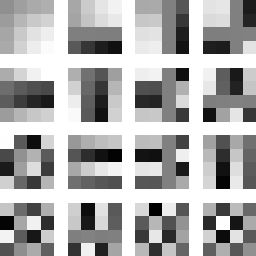
\includegraphics[width=0.15\linewidth]{./figures/mddt_sep_rdot_s4_p02.png}}
	\hfill
	\subfloat[sep. \acs{IPM} 6]
	{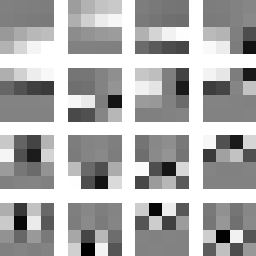
\includegraphics[width=0.15\linewidth]{./figures/mddt_sep_rdot_s4_p06.png}}
	\hfill
	\subfloat[sep. \acs{IPM} 10]
	{
\includegraphics[width=0.15\linewidth]{./figures/mddt_sep_rdot_s4_p10.png}}
	\hfill
	\subfloat[sep. \acs{IPM} 18]
	{
\includegraphics[width=0.15\linewidth]{./figures/mddt_sep_rdot_s4_p18.png}}
	\hfill
	\subfloat[sep. \acs{IPM} 26]
	{
\includegraphics[width=0.15\linewidth]{./figures/mddt_sep_rdot_s4_p26.png}}
	\\
	\subfloat[n-sep. \acs{IPM} 2]
	{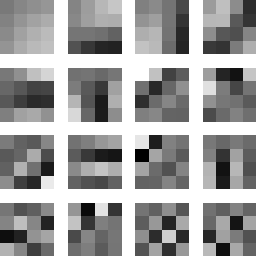
\includegraphics[width=0.15\linewidth]{./figures/mddt_nsep_rdot_s4_p02.png}}
	\hfill
	\subfloat[n-sep. \acs{IPM} 6]
	{\includegraphics[width=0.15\linewidth]{./figures/mddt_nsep_rdot_s4_p06.png}}
	\hfill
	\subfloat[n-sep. \acs{IPM} 10]
	{\includegraphics[width=0.15\linewidth]{./figures/mddt_nsep_rdot_s4_p10.png}}
	\hfill
	\subfloat[n-sep. \acs{IPM} 18]
	{\includegraphics[width=0.15\linewidth]{./figures/mddt_nsep_rdot_s4_p18.png}}
	\hfill
	\subfloat[n-sep. \acs{IPM} 26]
	{\includegraphics[width=0.15\linewidth]{./figures/mddt_nsep_rdot_s4_p26.png}}
	\caption{$4\times4$ separable and non-separable \acs{RDOT} for different \acsp{IPM}}
	\label{fig:rdot_4x4_bases}
\end{figure}

After having corroborated that the learning has output better performing
transforms in terms of distortion and sparseness, their implementation on top
of \ac{HEVC} is tested and discussed in the next section.

\subsection{\acs{MDDT} results on video coding}
\label{sub:mddt_results_on_video_coding}

The \ac{MDDT} systems designed in the previous tested have been used in
\ac{HEVC} using the common test conditions, defined by the
\ac{JCT-VC}~\cite{bossen-12-common-test-conditions}, for \ac{AI} and \ac{RA}
coding configurations.
The common test conditions consist in encoding each sequence at four different
\ac{QP} values (22, 27, 32, 37) and computing the average bit-rate savings
with regards to \ac{HEVC} using the \ac{BD}-rate metric.

\subsubsection{Bit-rate savings}
\label{ssub:mddt_bit_rate_savings}

Tables~\ref{tab:mddt_ai} and~\ref{tab:mddt_ra} contain the performances of
different \ac{MDDT} systems for \ac{AI} and \ac{RA} coding configurations,
respectively, for the different sequence classes of the \ac{HEVC} test set.
The last line of the table represents the average bit-rate savings for all
sequences (it does not correspond to the averaged bit-rate savings per class).

\begin{table}[tb]
	\centering
	\small
	\begin{tabularx}{\linewidth}{X|rr|rr|rr|rr|rr|rr}
		\multicolumn{1}{c}{} &
		\multicolumn{4}{c|}{$4\times4$} &
		\multicolumn{4}{c|}{$8\times8$} &
		\multicolumn{4}{c}{$4\times4$ \& $8\times8$} \\
		\cline{2-13}
		\multicolumn{1}{c}{} &
		\multicolumn{2}{c|} {sep} &
		\multicolumn{2}{c|} {non-sep} &
		\multicolumn{2}{c|} {sep} &
		\multicolumn{2}{c|} {non-sep} &
		\multicolumn{2}{c|} {sep} &
		\multicolumn{2}{c} {non-sep} \\
		\hline
		Cl. & KLT & RDOT & KLT & RDOT & KLT & RDOT & KLT & RDOT & KLT & RDOT & KLT & RDOT \\
		\hline\hline
		\centering A   &  0.08 &  0.12 & -0.18 & -0.17 & -0.96 & -0.98 & -1.60 & -1.56 & -0.88 & -0.90 & -1.63 & -1.60 \\
		\centering B   & -0.07 & -0.20 & -0.50 & -0.80 & -0.40 & -0.76 & -1.46 & -2.47 & -0.42 & -0.93 & -1.65 & -2.77 \\
		\centering C   & -0.18 & -0.60 & -1.46 & -2.47 & -0.42 & -0.82 & -2.40 & -4.03 & -0.51 & -1.33 & -3.09 & -5.15 \\
		\centering D   & -0.12 & -0.58 & -1.17 & -2.04 & -0.23 & -0.56 & -1.17 & -2.08 & -0.27 & -1.06 & -1.88 & -3.41 \\
		\centering E   &  0.39 &  0.35 & -0.07 & -0.45 & -0.92 & -1.20 & -2.11 & -2.91 & -0.57 & -0.95 & -1.83 & -3.00 \\
		\centering F   &  0.10 & -0.78 & -0.57 & -2.04 &  0.09 & -0.22 & -1.12 & -2.37 &  0.25 & -0.93 & -1.20 & -3.51 \\
		\hline\hline
		\centering Av. &  0.02 & -0.31 & -0.67 & -1.34 & -0.45 & -0.74 & -1.62 & -2.55 & -0.39 & -1.02 & -1.87 & -3.23 \\
	\end{tabularx}
	\caption{Average bit-rate savings (\%) for each \acs{HEVC} Class in \acs{AI}}
	\label{tab:mddt_ai}
\end{table}

\begin{table}[tb]
	\centering
	\small
	\begin{tabularx}{\linewidth}{X|rr|rr|rr|rr|rr|rr}
		\multicolumn{1}{c}{} &
		\multicolumn{4}{c|}{$4\times4$} &
		\multicolumn{4}{c|}{$8\times8$} &
		\multicolumn{4}{c}{$4\times4$ \& $8\times8$} \\
		\cline{2-13}
		\multicolumn{1}{c}{} &
		\multicolumn{2}{c|} {sep} &
		\multicolumn{2}{c|} {non-sep} &
		\multicolumn{2}{c|} {sep} &
		\multicolumn{2}{c|} {non-sep} &
		\multicolumn{2}{c|} {sep} &
		\multicolumn{2}{c} {non-sep} \\
		\hline
		Cl. & KLT & RDOT & KLT & RDOT & KLT & RDOT & KLT & RDOT & KLT & RDOT & KLT & RDOT \\
		\hline\hline
		\centering A   &  0.03 &  0.05 & -0.03 & -0.07 & -0.29 & -0.42 & -0.71 & -0.80 & -0.27 & -0.37 & -0.70 & -0.87 \\
		\centering B   &  0.00 & -0.10 & -0.26 & -0.51 & -0.24 & -0.46 & -0.86 & -1.42 & -0.25 & -0.55 & -0.99 & -1.63 \\
		\centering C   & -0.08 & -0.36 & -0.77 & -1.41 & -0.20 & -0.39 & -1.18 & -2.22 & -0.23 & -0.70 & -1.57 & -2.88 \\
		\centering D   & -0.03 & -0.25 & -0.50 & -1.05 & -0.08 & -0.25 & -0.53 & -1.05 & -0.11 & -0.50 & -0.88 & -1.73 \\
		\centering E   &  0.10 & -0.19 & -0.36 & -0.87 & -0.31 & -0.74 & -1.02 & -2.04 & -0.27 & -0.91 & -1.14 & -2.47 \\
		\centering F   &  0.07 & -0.59 & -0.29 & -1.26 &  0.08 & -0.10 & -0.50 & -1.42 &  0.18 & -0.65 & -0.56 & -2.21 \\
		\hline\hline
		\centering Av. &  0.01 & -0.24 & -0.37 & -0.85 & -0.17 & -0.38 & -0.80 & -1.47 & -0.16 & -0.60 & -0.97 & -1.93 \\
	\end{tabularx}
	\caption{Average bit-rate savings (\%) for each \acs{HEVC} Class in \acs{RA}}
	\label{tab:mddt_ra}
\end{table}

Three system configurations are reported:
a \ac{MDDT} system operating on $4\times4$ only \acp{TU}, $8\times8$ only
\acp{TU} and jointly on both sizes.
The first column of both tables refers to the separable \ac{KLT}-based
\ac{MDDT} for $4\times4$ \acp{TU}, which, as demonstrated
in~\cite{jain-75-nearest-neighbors, jain-76-klt-random-process}, corresponds
to the use of a \ac{DST}.
The average bit-rate savings with regards to \ac{HEVC} for this system are
insignficant since \ac{HEVC} already uses the \ac{DST} for those blocks.

The differences between both transform learning approaches (\ac{KLT} and
\ac{RDOT}) can be observed by looking at each pair of columns.
Results are very consistent with what was anticipated in the \ac{RDOT} metric
domain:
the \ac{RDOT}-based \ac{MDDT} outperforms the \ac{KLT} in every case
(separability, \ac{TU} size, class and coding configuration).

It is also worth-noticing the impact of separability:
non-separable configurations provide systematically higher bit-rate savings
than the separable ones, especially for those systems involving $8\times8$
\acp{TU}.

For the combined $4\times4$ and $8\times8$ system in \ac{AI} the bit-rate
savings are over 3\% and almost 2\% in \ac{RA}.
The \ac{KLT} systems are about one point below.
The detailed performances of the combined systems are included in
table~\ref{tab:detailed_mddt_bd_rate}.
Despite having used classes B and C for the transform learning, consistent
bit-rate savings are achieved across different resolutions among classes.
Moreover, classes D and E (not included in the learning set) present higher
bit-rate savings than class B.
It is also worth noticing that the \ac{RDOT} systems do not present losses for
any sequence, which is not the case for the \ac{KLT}.

\begin{table}[tb]
	\centering
	\small
	\begin{tabularx}{\textwidth}{c|X|rr|rr|rr|rr}
		\multicolumn{2}{c}{} &
		\multicolumn{8}{c}{$4\times4$ \& $8\times8$} \\
		\cline{3-10}
		\multicolumn{2}{c}{} &
		\multicolumn{4}{c|}{AI} &
		\multicolumn{4}{c}{RA} \\
		\cline{3-10}
		\multicolumn{2}{c}{} &
		\multicolumn{2}{c|}{sep} &
		\multicolumn{2}{c|}{non-sep} &
		\multicolumn{2}{c|}{sep} &
		\multicolumn{2}{c}{non-sep} \\
		\cline{2-10}
		\multicolumn{1}{c}{} & {Sequence} &
		{KLT} & {RDOT} & {KLT} & {RDOT} &
		{KLT} & {RDOT} & {KLT} & {RDOT} \\
		\hline\hline
		\multirow{5}{0.10\textwidth}{\centering Class A \scriptsize($2560\times1600$)}
		& NebutaFestival       & -0.55 & -0.37 & -0.72 &  -0.44 & -0.08 & -0.05 & -0.08 & -0.11 \\
		& PeopleOnStreet       & -1.17 & -1.31 & -2.53 &  -2.50 & -0.45 & -0.52 & -1.14 & -1.11 \\
		& SteamLocTrain        & -0.50 & -0.41 & -0.60 &  -0.55 &  0.03 &  0.00 & -0.11 & -0.30 \\
		& Traffic              & -1.33 & -1.49 & -2.66 &  -2.90 & -0.58 & -0.91 & -1.47 & -1.96 \\
		\cline{2-10}
		& Average              & -0.88 & -0.90 & -1.63 &  -1.60 & -0.27 & -0.37 & -0.70 & -0.87 \\
		\hline\hline
		\multirow{6}{0.10\textwidth}{\centering Class B \scriptsize($1920\times1080$)}
		& BasketballDrive      &  0.12 & -0.59 & -1.12 &  -2.82 & -0.25 & -0.42 & -1.24 & -1.85 \\
		& BQTerrace            &  0.27 & -0.85 & -2.19 &  -4.62 & -0.05 & -0.63 & -1.28 & -2.45 \\
		& Cactus               & -0.92 & -1.47 & -2.28 &  -3.41 & -0.34 & -0.78 & -1.19 & -2.16 \\
		& Kimono1              & -0.38 & -0.47 & -0.95 &  -1.11 & -0.03 & -0.21 & -0.31 & -0.48 \\
		& ParkScene            & -1.19 & -1.28 & -1.69 &  -1.92 & -0.58 & -0.72 & -0.91 & -1.23 \\
		\cline{2-10}
		& Average              & -0.42 & -0.93 & -1.65 &  -2.77 & -0.25 & -0.55 & -0.99 & -1.63 \\
		\hline\hline
		\multirow{5}{0.10\textwidth}{\centering Class C \scriptsize($832\times480$)}
		& BasketballDrill      & -1.20 & -1.77 & -7.92 & -11.88 & -0.55 & -0.94 & -3.79 & -6.34 \\
		& BQMall               &  0.03 & -1.14 & -0.83 &  -2.58 &  0.12 & -0.58 & -0.33 & -1.47 \\
		& PartyScene           & -0.04 & -1.15 & -1.00 &  -2.56 & -0.07 & -0.68 & -0.74 & -1.75 \\
		& RaceHorses           & -0.84 & -1.26 & -2.60 &  -3.57 & -0.40 & -0.58 & -1.42 & -1.97 \\
		\cline{2-10}
		& Average              & -0.51 & -1.33 & -3.09 &  -5.15 & -0.23 & -0.70 & -1.57 & -2.88 \\
		\hline\hline
		\multirow{5}{0.10\textwidth}{\centering Class D \scriptsize($416\times240$)}
		& BasketballPass       & -0.11 & -0.94 & -1.47 &  -3.12 & -0.12 & -0.52 & -0.96 & -1.78 \\
		& BlowingBubbles       & -0.05 & -0.97 & -1.80 &  -3.49 & -0.07 & -0.52 & -0.93 & -1.90 \\
		& BQSquare             &  0.09 & -1.00 & -0.91 &  -2.69 &  0.08 & -0.53 & -0.24 & -1.40 \\
		& RaceHorses           & -1.00 & -1.34 & -3.36 &  -4.34 & -0.34 & -0.43 & -1.40 & -1.84 \\
		\cline{2-10}
		& Average              & -0.27 & -1.06 & -1.88 &  -3.41 & -0.11 & -0.50 & -0.88 & -1.73 \\
		\hline\hline
		\multirow{4}{0.10\textwidth}{\centering Class E \scriptsize($1280\times720$)}
		& FourPeople           & -1.19 & -1.51 & -2.41 &  -3.20 & -0.59 & -1.23 & -1.52 & -2.54 \\
		& Johnny               & -0.33 & -0.75 & -1.52 &  -2.82 & -0.12 & -0.78 & -0.97 & -2.37 \\
		& KristenAndSara       & -0.18 & -0.59 & -1.56 &  -2.99 & -0.12 & -0.73 & -0.94 & -2.50 \\
		\cline{2-10}
		& Average              & -0.57 & -0.95 & -1.83 & -3.00 & -0.27 & -0.91 & -1.14 & -2.47 \\
		\hline\hline
		\multirow{5}{0.10\textwidth}{\centering Class F \scriptsize(various resolutions)}
		& BasketDrillText      & -0.84 & -1.80 & -6.14 &  -9.96 & -0.48 & -0.88 & -3.15 & -5.57 \\
		& ChinaSpeed           &  0.44 & -0.81 & -0.02 &  -1.81 &  0.17 & -0.43 & -0.08 & -0.95 \\
		& SlideEditing         &  0.68 & -0.57 &  0.98 &  -0.46 &  0.52 & -0.76 &  0.77 & -0.76 \\
		& SlideShow            &  0.73 & -0.55 &  0.37 &  -1.81 &  0.50 & -0.53 &  0.23 & -1.55 \\
		\cline{2-10}
		& Average              &  0.25 & -0.93 & -1.20 &  -3.51 & 0.18  & -0.65 & -0.56 & -2.21 \\
		\hline\hline
		All Sequences
		& Overall          & -0.39 & -1.02 & -1.87 &  -3.23 & -0.16 & -0.60 & -0.97 & -1.93 \\
	\end{tabularx}
	\caption{Detailed bit-rate savings (\%) for combined $4\times4$ \& $8\times8$
	\acs{MDDT} systems}
	\label{tab:detailed_mddt_bd_rate}
\end{table}

A remarkable point stands out of the test set: the \emph{BasketballDrill}
sequence from class C, with bit-rate savings of almost 12\% using the
non-separable \ac{RDOT} in \ac{AI}.
This is due to the fact that this sequence presents strong directional
patterns that cannot be dealt with separable transforms.
Almost all the performance is lost when using separable systems.
For illustrative purposes, figure~\ref{fig:detailed_mddt_bd_rate} represents
graphically the results from table~\ref{tab:detailed_mddt_bd_rate}.
The behaviour in the \ac{RA} coding configuration is very similar to the
\ac{AI}, with the bit-rate savings in \ac{RA} being around two thirds of those
in \ac{AI}.

\begin{figure}[tp]
	\centering
	\subfloat[\acs{AI} coding configuration]
	{\ifthenelse{\usepdfs = 0}
	{
\begin{tikzpicture}
	\pgfplotsset{/tikz/font={\small}}
	\begin{axis}[
		grid=both,
		width=1.0\textwidth,
		height=0.3\textheight,
		x tick label style={
		/pgf/number format/1000 sep=},
		ytick={0,-2,...,-12},
		y tick label style={
			/pgf/number format/.cd,
			fixed,
			fixed zerofill,
			precision=1,
		},
		y dir=reverse,
		ymax=1, ymin=-12,
		ylabel={Y BD-rate (\%)},
		% enlargelimits=0.15,
		enlarge y limits=false,
		enlarge x limits=0.04,
		legend style={at={(0.5,-0.45)},
		anchor=north,legend columns=-1},
		ybar interval,
		% bar width=1pt,
		xtick=data,
		xtick align=inside,
		% nodes near coords,
		% xlabel={Sequences},
		% xlabel near ticks,
		symbolic x coords={
			NebutaFestival,
			PeopleOnStreet,
			SteamLocTrain,
			Traffic,
			BasketballDrive,
			BQTerrace,
			Cactus,
			Kimono1,
			ParkScene,
			BasketballDrill,
			BQMall,
			PartyScene,
			RaceHorses\_480p,
			BasketballPass,
			BlowingBubbles,
			BQSquare,
			RaceHorses\_240p,
			FourPeople,
			Johnny,
			KristenAndSara,
			BasketDrillText,
			ChinaSpeed,
			SlideEditing,
			SlideShow,
			Overall,
		},
		x tick label style={rotate=-60,anchor=west},
		]

		\addlegendentry{Sep KLT AI}
		\addplot coordinates {
		(NebutaFestival,   -0.55)
		(PeopleOnStreet,   -1.17)
		(SteamLocTrain,    -0.50)
		(Traffic,          -1.33)
		(BasketballDrive,   0.12)
		(BQTerrace,         0.27)
		(Cactus,           -0.92)
		(Kimono1,          -0.38)
		(ParkScene,        -1.19)
		(BasketballDrill,  -1.20)
		(BQMall,            0.03)
		(PartyScene,       -0.04)
		(RaceHorses\_480p, -0.84)
		(BasketballPass,   -0.11)
		(BlowingBubbles,   -0.05)
		(BQSquare,          0.09)
		(RaceHorses\_240p, -1.00)
		(FourPeople,       -1.19)
		(Johnny,           -0.33)
		(KristenAndSara,   -0.18)
		(BasketDrillText,  -0.84)
		(ChinaSpeed,        0.44)
		(SlideEditing,      0.68)
		(SlideShow,         0.73)
		(Overall,          -0.39)
		};

		\addlegendentry{Sep RDOT AI}
		\addplot coordinates {
		(NebutaFestival,   -0.37)
		(PeopleOnStreet,   -1.31)
		(SteamLocTrain,    -0.41)
		(Traffic,          -1.49)
		(BasketballDrive,  -0.59)
		(BQTerrace,        -0.85)
		(Cactus,           -1.47)
		(Kimono1,          -0.47)
		(ParkScene,        -1.28)
		(BasketballDrill,  -1.77)
		(BQMall,           -1.14)
		(PartyScene,       -1.15)
		(RaceHorses\_480p, -1.26)
		(BasketballPass,   -0.94)
		(BlowingBubbles,   -0.97)
		(BQSquare,         -1.00)
		(RaceHorses\_240p, -1.34)
		(FourPeople,       -1.51)
		(Johnny,           -0.75)
		(KristenAndSara,   -0.59)
		(BasketDrillText,  -1.80)
		(ChinaSpeed,       -0.81)
		(SlideEditing,     -0.57)
		(SlideShow,        -0.55)
		(Overall,          -1.02)
		};

		\addlegendentry{N-sep KLT AI}
		\addplot coordinates {
		(NebutaFestival,  -0.72)
		(PeopleOnStreet,  -2.53)
		(SteamLocTrain,   -0.60)
		(Traffic,         -2.66)
		(BasketballDrive, -1.12)
		(BQTerrace,       -2.19)
		(Cactus,          -2.28)
		(Kimono1,         -0.95)
		(ParkScene,       -1.69)
		(BasketballDrill, -7.92)
		(BQMall,          -0.83)
		(PartyScene,      -1.00)
		(RaceHorses\_480p,-2.60)
		(BasketballPass,  -1.47)
		(BlowingBubbles,  -1.80)
		(BQSquare,        -0.91)
		(RaceHorses\_240p,-3.36)
		(FourPeople,      -2.41)
		(Johnny,          -1.52)
		(KristenAndSara,  -1.56)
		(BasketDrillText, -6.14)
		(ChinaSpeed,      -0.02)
		(SlideEditing,     0.98)
		(SlideShow,        0.37)
		(Overall,         -1.87)
		};

		\addlegendentry{N-sep RDOT AI}
		\addplot coordinates {
		(NebutaFestival,   -0.44)
		(PeopleOnStreet,   -2.50)
		(SteamLocTrain,    -0.55)
		(Traffic,          -2.90)
		(BasketballDrive,  -2.82)
		(BQTerrace,        -4.62)
		(Cactus,           -3.41)
		(Kimono1,          -1.11)
		(ParkScene,        -1.92)
		(BasketballDrill, -11.88)
		(BQMall,           -2.58)
		(PartyScene,       -2.56)
		(RaceHorses\_480p, -3.57)
		(BasketballPass,   -3.12)
		(BlowingBubbles,   -3.49)
		(BQSquare,         -2.69)
		(RaceHorses\_240p, -4.34)
		(FourPeople,       -3.20)
		(Johnny,           -2.82)
		(KristenAndSara,   -2.99)
		(BasketDrillText,  -9.96)
		(ChinaSpeed,       -1.81)
		(SlideEditing,     -0.46)
		(SlideShow,        -1.81)
		(Overall,          -3.23)
		};

	\end{axis}
\end{tikzpicture}
}
	{\includegraphics{./figures/mddt_perf_ai_plot.pdf}}}

	\subfloat[\acs{RA} coding configuration]
	{\ifthenelse{\usepdfs = 0}
	{
\begin{tikzpicture}
	\pgfplotsset{/tikz/font={\small}}
	\begin{axis}[
		grid=both,
		width=1.0\textwidth,
		height=0.3\textheight,
		x tick label style={
		/pgf/number format/1000 sep=},
		ytick={0,...,-7},
		y tick label style={
			/pgf/number format/.cd,
			fixed,
			fixed zerofill,
			precision=1,
		},
		y dir=reverse,
		ymax=1, ymin=-7,
		ylabel={Y BD-rate (\%)},
		% enlargelimits=0.15,
		enlarge y limits=false,
		enlarge x limits=0.04,
		legend style={at={(0.5,-0.45)},
		anchor=north,legend columns=-1},
		ybar interval,
		% bar width=1pt,
		xtick=data,
		xtick align=inside,
		% nodes near coords,
		% xlabel={Sequences},
		% xlabel near ticks,
		symbolic x coords={
			NebutaFestival,
			PeopleOnStreet,
			SteamLocTrain,
			Traffic,
			BasketballDrive,
			BQTerrace,
			Cactus,
			Kimono1,
			ParkScene,
			BasketballDrill,
			BQMall,
			PartyScene,
			RaceHorses\_480p,
			BasketballPass,
			BlowingBubbles,
			BQSquare,
			RaceHorses\_240p,
			FourPeople,
			Johnny,
			KristenAndSara,
			BasketDrillText,
			ChinaSpeed,
			SlideEditing,
			SlideShow,
			Overall,
		},
		x tick label style={rotate=-60,anchor=west},
		]

		\addlegendentry{Sep. KLT RA}
		\addplot coordinates {
		(NebutaFestival,   -0.08)
		(PeopleOnStreet,   -0.45)
		(SteamLocTrain,     0.03)
		(Traffic,          -0.58)
		(BasketballDrive,  -0.25)
		(BQTerrace,        -0.05)
		(Cactus,           -0.34)
		(Kimono1,          -0.03)
		(ParkScene,        -0.58)
		(BasketballDrill,  -0.55)
		(BQMall,            0.12)
		(PartyScene,       -0.07)
		(RaceHorses\_480p, -0.40)
		(BasketballPass,   -0.12)
		(BlowingBubbles,   -0.07)
		(BQSquare,          0.08)
		(RaceHorses\_240p, -0.34)
		(FourPeople,       -0.59)
		(Johnny,           -0.12)
		(KristenAndSara,   -0.12)
		(BasketDrillText,  -0.48)
		(ChinaSpeed,        0.17)
		(SlideEditing,      0.52)
		(SlideShow,         0.50)
		(Overall,          -0.16)
		};

		\addlegendentry{Sep. RDOT RA}
		\addplot coordinates {
		(NebutaFestival,   -0.05)
		(PeopleOnStreet,   -0.52)
		(SteamLocTrain,     0.00)
		(Traffic,          -0.91)
		(BasketballDrive,  -0.42)
		(BQTerrace,        -0.63)
		(Cactus,           -0.78)
		(Kimono1,          -0.21)
		(ParkScene,        -0.72)
		(BasketballDrill,  -0.94)
		(BQMall,           -0.58)
		(PartyScene,       -0.68)
		(RaceHorses\_480p, -0.58)
		(BasketballPass,   -0.52)
		(BlowingBubbles,   -0.52)
		(BQSquare,         -0.53)
		(RaceHorses\_240p, -0.43)
		(FourPeople,       -1.23)
		(Johnny,           -0.78)
		(KristenAndSara,   -0.73)
		(BasketDrillText,  -0.88)
		(ChinaSpeed,       -0.43)
		(SlideEditing,     -0.76)
		(SlideShow,        -0.53)
		(Overall,          -0.60)
		};

		\addlegendentry{N-sep. KLT RA}
		\addplot coordinates {
		(NebutaFestival,   -0.08)
		(PeopleOnStreet,   -1.14)
		(SteamLocTrain,    -0.11)
		(Traffic,          -1.47)
		(BasketballDrive,  -1.24)
		(BQTerrace,        -1.28)
		(Cactus,           -1.19)
		(Kimono1,          -0.31)
		(ParkScene,        -0.91)
		(BasketballDrill,  -3.79)
		(BQMall,           -0.33)
		(PartyScene,       -0.74)
		(RaceHorses\_480p, -1.42)
		(BasketballPass,   -0.96)
		(BlowingBubbles,   -0.93)
		(BQSquare,         -0.24)
		(RaceHorses\_240p, -1.40)
		(FourPeople,       -1.52)
		(Johnny,           -0.97)
		(KristenAndSara,   -0.94)
		(BasketDrillText,  -3.15)
		(ChinaSpeed,       -0.08)
		(SlideEditing,      0.77)
		(SlideShow,         0.23)
		(Overall,          -0.97)
		};

		\addlegendentry{N-sep. RDOT RA}
		\addplot coordinates {
		(NebutaFestival,   -0.11)
		(PeopleOnStreet,   -1.11)
		(SteamLocTrain,    -0.30)
		(Traffic,          -1.96)
		(BasketballDrive,  -1.85)
		(BQTerrace,        -2.45)
		(Cactus,           -2.16)
		(Kimono1,          -0.48)
		(ParkScene,        -1.23)
		(BasketballDrill,  -6.34)
		(BQMall,           -1.47)
		(PartyScene,       -1.75)
		(RaceHorses\_480p, -1.97)
		(BasketballPass,   -1.78)
		(BlowingBubbles,   -1.90)
		(BQSquare,         -1.40)
		(RaceHorses\_240p, -1.84)
		(FourPeople,       -2.54)
		(Johnny,           -2.37)
		(KristenAndSara,   -2.50)
		(BasketDrillText,  -5.57)
		(ChinaSpeed,       -0.95)
		(SlideEditing,     -0.76)
		(SlideShow,        -1.55)
		(Overall,          -1.93)
		};

	\end{axis}
\end{tikzpicture}
}
	{\includegraphics{./figures/mddt_perf_ra_plot.pdf}}}

	\caption{Bit-rate savings for combined $4\times4$ \& $8\times8$ \acs{MDDT}
	systems}
	\label{fig:detailed_mddt_bd_rate}
\end{figure}

As a reminder, all transforms learnt for the presented \ac{MDDT} systems have
used residuals issued from \ac{AI} coding configurations and have only been
enabled for intra coded residuals in \ac{HEVC}.
Nonetheless, around two thirds of the bit-rate savings achieved for the
\ac{AI} coding configurations have been achieved in \ac{RA}.
This is due to the fact that I-frames, and intra coded blocks in \ac{RA} are
of higher quality, and serve, therefore, as better references to derive the
temporal predictions.

A final comment on the designed transforms regarding the scanning of the
transformed coefficients:
the transform base vectors for each \ac{IPM} have been sorted taking into
account the scanning that \ac{HEVC} performs implicitly, illustrated in
figure~\ref{fig:mdcs}.
For non-separable transforms, base vectors can be placed in any order, but
separable transforms does not have this freedom, as such, an adapted scanning
matrix is needed to make sure the transform coefficients are properly sorted.

\subsubsection{Coding complexity}
\label{ssub:mddt_coding_complexity}

Regarding the complexity of the system, the increase in the encoding and
decoding time is only due to the lack of fast algorithms for \acp{KLT} and
\acp{RDOT}.
Due to the way the quad-tree partitioning works in \ac{HEVC}, if, for
instance, a $16\times16$ \ac{TU} provides a better rate-distortion trade-off
than splitting it into $8\times8$ \acp{TU}, the $4\times4$ will not be
explored.
Since the \ac{MDDT} system improves $4\times4$ and $8\times8$ \acp{TU}, it
becomes more likely that splitting a $16\times16$ \ac{TU} into four $8\times8$
\acp{TU} works better than not splitting.
In that case, the $4\times4$ \acp{TU} will also be explored, which will lead
to an increase in complexity with regards to \ac{HEVC}, as more coding
possibilities are being explored.
Table~\ref{tab:mddt_summary} summarises the coding complexity for \ac{MDDT}
systems using separable and non-separable transforms for $4\times4$ and
$8\times8$ \acp{TU}.
The complexity for \ac{KLT} and \ac{RDOT} based systems is equivalent, since
transforms are performed as generic matrix multiplications.
As seen in \S\ref{sub:separability}, the number of operations required for a
non-separable transform is about $N$ times the amount for separable
transforms, with $N$ being the \ac{TU} size.
For $4\times4$ \acp{TU}, the complexity in both coding and decoding times
remains approximately the same as that of \ac{HEVC}.
However, for larger \acp{TU}, the differences due to fast algorithms start
becoming more noticeable.

\begin{table}[tb]
	\centering
	\small
	\begin{tabular}{c|rr|rr|rr}
		\multicolumn{1}{c}{}
		& \multicolumn{2}{c|}{$4\times4$}
		& \multicolumn{2}{c|}{$8\times8$}
		& \multicolumn{2}{c}{$4\times4$ \& $8\times8$} \\
		\multicolumn{1}{c}{}
		& \multicolumn{1}{c}{sep} & \multicolumn{1}{c|}{non-sep}
		& \multicolumn{1}{c}{sep} & \multicolumn{1}{c|}{non-sep}
		& \multicolumn{1}{c}{sep} & \multicolumn{1}{c}{non-sep} \\
		\hline\hline
		Y \acs{BD}-rate & -0.31\% & -1.34\% & -0.74\% & -2.55\% & -1.02\% & -3.23\% \\
		Encoding  & 101\% & 102\% & 107\% & 111\% & 108\% & 112\% \\
		Decoding  & 101\% & 102\% & 103\% & 115\% & 105\% & 120\% \\
		\acs{ROM} & \SI{1.64}{\kilo B} & \SI{8.75}{\kilo B} &
				\SI{6.56}{\kilo B} & \SI{140.00}{\kilo B} &
				\SI{8.20}{\kilo B} & \SI{148.75}{\kilo B}\\
	\end{tabular}
	\caption{Summary of \acs{RDOT}-based \acs{MDDT} systems compared to
	\acs{HEVC} in \acs{AI}}
	\label{tab:mddt_summary}
\end{table}

\subsubsection{\acs{MDDT} storage requirements}
\label{ssub:mddt_storage_requirements}
\index{ROM}

The transforms used in the \ac{MDDT} system are, not describable with a
mathematical formula unlike the \ac{DCT} and the \ac{DST}.
As such, additional memory is required to store these transforms and make them
available to the encoder and the decoder.
Each transform coefficient has been quantised to 1 byte by rounding it to the
nearest integer.
More advanced quantisation techniques could have been implemented that would
lead to lower degradations~\cite{britanak-06-dct-and-dst}.
The rounding method does not guarantee that the transform remains orthogonal
and that the energy preservation property in the \ac{RDOT} is retained,
although experiments done with this quantisation show that observed losses are
in the order of 0.2 \ac{BD}-rate points.
Taking all of this into account, the storage requirements for a non-separable
transform for $N\times N$ \acp{TU} is:
\begin{equation}
	\acs{ROM}_{\text{non-sep}} =
	N^2 \cdot N^2 \cdot \frac{\SI{1}{\kilo B}}{\SI{1024}{B}} \cdot M
	\label{eqn:rom_nsep}
\end{equation}
The needed \acs{ROM} for separable transforms is:
\begin{equation}
	\acs{ROM}_{\text{sep}} =
	3 \cdot N \cdot N \cdot \frac{\SI{1}{\kilo B}}{\SI{1024}{B}} \cdot M
	\label{eqn:rom_sep}
\end{equation}
Where the number of \acp{IPM} $M$ is 35 for the \ac{MDDT} system.
Sorting the transform base vectors in the proper order is essential to assist
the entropy coding~\cite{ye-08-intra-directional-scanning-mddt}.
For this reason, there is a factor 3 for the \acs{ROM} requirements in the
separable case: horizontal transform, vertical transform and scanning matrix
for each pair of transforms.
The non-separable transforms do not need a scanning matrix, since the base
vectors can be sorted to output the signal with an appropriate coefficients
order.
Table~\ref{tab:mddt_summary} contains the \acs{ROM} requirements for the
\ac{MDDT} systems in both separable and non-separable designs.
This table illustrates the drawback of using non-separable transforms
regarding the storage.
Even the \ac{MDDT} system using only non-separable transforms for $4\times4$
\acp{TU} needs more \acs{ROM} than the complete separable \ac{MDDT} system
making use of both sizes.

\section{Conclusions}
\label{sec:mddt_conclusions}

Transform designs presented in Chapter~\ref{cha:transform_coding}, namely the
\ac{KLT} and the \ac{RDOT}, have been evaluated through the \ac{MDDT}, a
technique for intra coded blocks that consists in designing an adapted
transform per \ac{IPM}.
During the learning phase, the \ac{RDOT} metric has presented coherent results
with the knowledge acquired from literature regarding the \ac{KLT}, \ac{DCT}
and \ac{DST}.
These transforms have been evaluated using the \ac{RDOT} metric and have been
corroborated by the results obtained in the \ac{BD}-rate domain:
for intra prediction residuals, the \ac{DST}-VII has a better \ac{BD}-rate
score than the \ac{DCT}-II, and so does using the \ac{RDOT} metric.

The designed transforms have been tested in a modified version of \ac{HEVC}
using the \ac{MDDT} technique.
Non-separable transforms present a significant improvement in terms of
bit-rate savings over their separable counterparts.
Moreover, the \ac{RDOT} design approach has provided better results in terms
of \ac{BD}-rate than the \ac{KLT} all over the tested sequences, with no
losses for any of them.
Bit-rate savings between around 2--3\% are achieved when using the
\ac{RDOT}-based \ac{MDDT}, which validate the transfom design over the
\ac{KLT}-based design, providing bit-rate savings around 1 point below.
Consequently, the \ac{KLT} will no longer be considered in the upcoming
sections, only systems designed using the \ac{RDOT} metric will be considered.

The complexity of the \ac{MDDT} systems remains comparable to that of
\ac{HEVC}, since the modification only implies that default transform is
replaced with an adapted one.
Therefore, the increase in complexity is only due to the fact that transforms
are implemented as matrix multiplications due to the lack of fast algorithms
for general orthogonal transforms.

The following Chapter presents an improvement of the \ac{MDDT}, which will
allow transforms to be more adapted to intra prediction residuals and provide
new coding alternatives to \ac{HEVC}.

\chapter{The mode-dependent transform competition system}
\label{cha:mdtc}
\chaptertoc

\section{Introduction}
\label{sec:introduction_mdtc}
\index{MDDT}
\index{MDTC}

Chapter~\ref{cha:mddt} revisited the existing \acf{MDDT} technique, its
origins and motivation, and explained how it was discarded in the final
\ac{HEVC} standard in favour of a more simplified approach using the \ac{DST}.
However, the \ac{MDDT} technique has good potential in bit-rate savings when
used with \acp{RDOT}, especially in their non-separable design.

This Chapter is focused on improving upon the \ac{MDDT} technique by
increasing the number of available transforms.
The main idea is to provide a fixed number of transforms per \acf{IPM} that
compete against each other in the \ac{RDO} loop, in the same ways as block
sizes and \acp{IPM} do.
This implies that, for a given block size and \ac{IPM}, there is no longer a
unique transform, but a set of them, and the encoder selects the one that
provides the best trade-off in terms of rate-distortion.
This evolution of the \ac{MDDT} system has been named \ac{MDTC} system.

Transform competition is not an entirely new concept in \ac{HEVC}.
A rudimentary form of competition is present for $4\times4$ intra predicted
luma residuals:
the choice between using the \ac{DST}-VII and not using a transform at all
already exists.
This behaviour is controlled by the
\texttt{transform\_skip\_flag}~\cite{JCTVC-F077, JCTVC-H0208}.

Some work on transform competition has been carried out
in~\cite{arrufat-14-transform-competition-rdot,fengzou-13-rdot-lloyd-intra}.
The main difference is that, in this Chapter, each \ac{IPM} has its own
transform sets instead of a common set for all modes.
The approach from~\cite{fengzou-13-rdot-lloyd-intra} uses the same transforms
for all \acp{IPM}.
The block size and \ac{IPM} decision is based on the default \ac{HEVC}
transforms, then the residual is consequently transformed with the transform
that provides the best trade-off in terms of rate-distortion.

Further work on different mode-dependent tools for video coding have been
explored in~\cite{ma-13-mode-dependent-tools-video-coding}, notably ways of
simplifying and improving the \ac{MDDT} system by adding re-orderings in the
residuals and additional transforms after the main transform.

Early work on \ac{MDTC} systems closely related to this Chapter has been
presented in~\cite{arrufat-15-mdtc}.

\section{Multiple transform design using the \acs{RDOT} metric}
\label{sec:multiple_transform_design}

\subsection{\acs{HEVC} compatibility}
\label{sub:mdtc_hevc_compatibility}
\index{HEVC}

Since the main purpose of the transforms in \ac{HEVC} is to compact the energy
of the signal in order to increase the bit-rate savings, the design process is
developed as follows:
the default \ac{HEVC} transforms for $4\times4$ and $8\times8$ luma blocks
(the \ac{DST} and \ac{DCT}, respectively) are kept and a number of additional
transforms are learnt to capture those residuals for which \ac{HEVC}
transforms are not adapted to.
This choice has been made to guarantee a level of backward compatibility with
\ac{HEVC}, where the original coding choices are still available when using
the \ac{MDTC} system.

\subsection{The learning algorithm}
\label{sub:mdtc_learning_algorithm}

The chosen transform design is the \ac{RDOT}, since, as demonstrated in the
previous Chapter, it provides significant improvements in terms of bit-rate
savings with respect to the \ac{KLT}.
However, in this Chapter, more than one \ac{RDOT} will be learnt per \ac{IPM},
in stead of one, using the same learning set:
residuals issued from an \ac{AI} \ac{HEVC} coding of classes B and C from the
\ac{HEVC} test set, grouped by \ac{IPM}.
For each \ac{IPM}, $2^N$ transforms are learnt, in addition to the \ac{HEVC}
default transforms (for compatibility reasons).
Algorithm~\ref{alg:clustering} describes how the learning has been carried out
in each \ac{IPM}.
Assuming the desired outputs are $2^N$ additional transforms, the performed
steps are:
\begin{enumerate}
	\item Initial random classification of the residuals into $1+2^N$ classes.
	\item For the $2^N$ classes that are not assigned to the \ac{HEVC}
		transform, learn a separable or non-separable transform, depending on
		the desired configuration.
	\item Evaluate each residual using the RDOT metric and assign it to the
		transform that minimises the value.
	\item Repeat steps 2 and 3 until convergence.
\end{enumerate}
An example for $N=1\Rightarrow2^N=2$ additional transforms is provided in
figure~\ref{fig:clustering}.
This algorithm is subject to improvements, since the initial conditions are
difficult to define.
Consequently, in order to increase the confidence level of not ending up into
a local minimum, several runs per learning are done with different
initialisations.

\begin{algorithm}
	\small
	\SetKwData{append}{append}
	\SetKwInOut{Input}{input}
	\SetKwInOut{Output}{output}
	\Input{Residuals $\x$ from a given \acl{IPM}}
	\Output{Set of $2^N$ \acp{RDOT} $A_n$}
	\BlankLine%
	Initial random classification into $1+2^N$ classes
	\BlankLine%
	\While{!convergence}
	{
			\For{$n=1$ \KwTo{} $2^N$}
			{
				Learn a \ac{RDOT} on $\text{Class}_n$
				using~\eqref{eqn:rdot-nsep} or~\eqref{eqn:rdot-sep}, depending
				on separability
			}
			\ForEach{block $\x$}
			{
				\For{$n=0$ \KwTo{} $2^N$}
				{
					$\delta_n =
					{\Vert \x - \A^T_n\c\Vert}^2 + \lambda{\Vert\c\Vert}_0$
				}
				$\displaystyle n^* = \text{arg}\min\limits_n(\delta_n)$\\
				$\text{Class}_{n^*}$.\append($\x$)
			}
	}
	\caption{Multiple transform design}
	\label{alg:clustering}
\end{algorithm}

\begin{figure}[tp]
	\centering
	\ifthenelse{\usepdfs = 0}
	{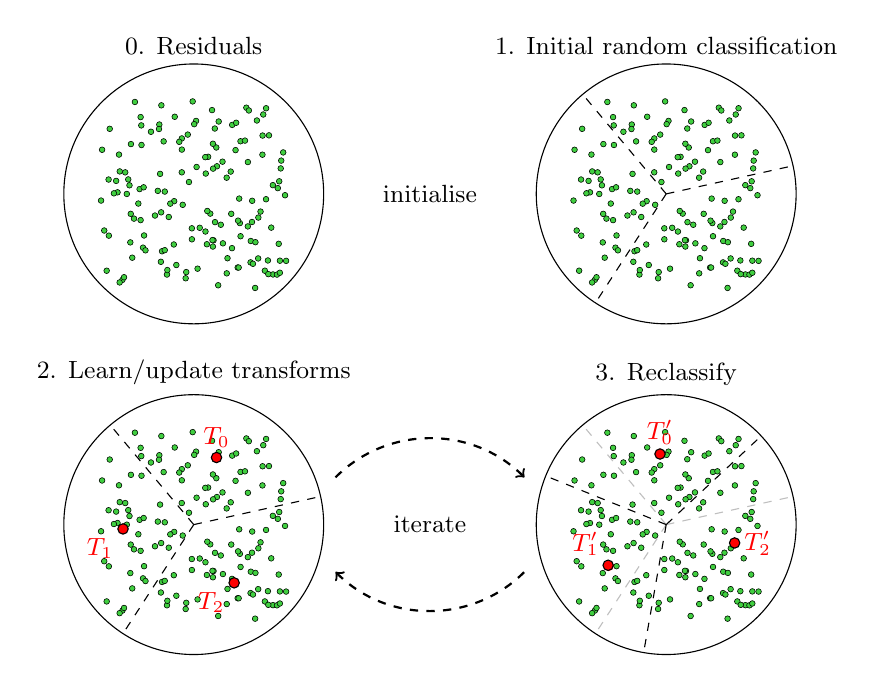
\begin{tikzpicture}[scale=0.6]
	\pgfplotsset{/tikz/font={\small}}

	% add this node to prevent pdfcrop from cropping left circles
	\draw[black!0] (-2.77,0) node {};

	\pgfmathsetseed{5}
	\foreach \i in {1,2,...,150}{
		\pgfmathsetmacro{\x}{(rand*0.5 + 1)*4 - 4.0}
		\pgfmathsetmacro{\y}{(rand*0.5 + 1)*4 - 4.0}
		\pgfmathsetmacro{\opacVal}{rand*0+1}
		\filldraw [black!25!green!75, opacity = \opacVal] (\x,\y) circle (0.05);
		\draw[very thin] (\x,\y) circle (0.06);
	}

	\draw (0,0) circle [radius=2.75];

	\draw (90:2.75) node [above] {0. Residuals};
	\pgfmathsetseed{5}
	\foreach \i in {1,2,...,150}{
		\pgfmathsetmacro{\x}{(rand*0.5 + 1)*4 - 4.0}
		\pgfmathsetmacro{\y}{(rand*0.5 + 1)*4 - 4.0}
		\pgfmathsetmacro{\opacVal}{rand*0+1}
		\filldraw [black!25!green!75, opacity = \opacVal] (\x+10,\y) circle (0.05);
		\draw[very thin] (\x+10,\y) circle (0.06);
	}

	\draw (10,0) circle [radius=2.75];
	\draw[dashed] (10,0) --++ (12.5:2.75);
	\draw[dashed] (10,0) --++ (130:2.75);
	\draw[dashed] (10,0) --++ (237:2.75);

	\draw (10,0)++(90:2.75) node [above] {1. Initial random classification};

	\draw (5,0) node {initialise};

	%%%%%%%%%
	\def\yoffset{-7}

	\pgfmathsetseed{5}
	\foreach \i in {1,2,...,150}{
		\pgfmathsetmacro{\x}{(rand*0.5 + 1)*4 - 4.0}
		\pgfmathsetmacro{\y}{(rand*0.5 + 1)*4 - 4.0 + \yoffset}
		\pgfmathsetmacro{\opacVal}{rand*0+1}
		\filldraw [black!25!green!75, opacity = \opacVal] (\x,\y) circle (0.05);
		\draw[very thin] (\x,\y) circle (0.06);
	}

	\draw (0,\yoffset) circle [radius=2.75];
	\draw[dashed] (0,\yoffset) --++ (12.5:2.75);
	\draw[dashed] (0,\yoffset) --++ (130:2.75);
	\draw[dashed] (0,\yoffset) --++ (237:2.75);

	\filldraw [red] (0,\yoffset)++(71.25:1.5) circle (0.1) node [above] (T0) {$T_0$};
	\draw[thin] (0,\yoffset)++(71.25:1.5) circle (0.11);

	\filldraw [red] (0,\yoffset)++(183.5:1.5) circle (0.1) node [below left] (T1) {$T_1$};
	\draw[thin] (0,\yoffset)++(183.5:1.5) circle (0.11);

	\filldraw [red] (0,\yoffset)++(304.75:1.5) circle (0.1) node [below left] (T2) {$T_2$};
	\draw[thin] (0,\yoffset)++(304.75:1.5) circle (0.11);

	\draw (0,\yoffset)++(90:2.75) node [above] {2. Learn/update transforms};
	\pgfmathsetseed{5}
	\foreach \i in {1,2,...,150}{
		\pgfmathsetmacro{\x}{(rand*0.5 + 1)*4 - 4.0}
		\pgfmathsetmacro{\y}{(rand*0.5 + 1)*4 - 4.0 + \yoffset}
		\pgfmathsetmacro{\opacVal}{rand*0+1}
		\filldraw [black!25!green!75, opacity = \opacVal] (\x+10,\y) circle (0.05);
		\draw[very thin] (\x+10,\y) circle (0.06);
	}

	\draw (10,\yoffset) circle [radius=2.75];
	\draw[dashed, opacity=0.25] (10,\yoffset) --++ (12.5:2.75);
	\draw[dashed, opacity=0.25] (10,\yoffset) --++ (130:2.75);
	\draw[dashed, opacity=0.25] (10,\yoffset) --++ (237:2.75);

	\draw[dashed] (10,\yoffset) --++ (43:2.75);
	\draw[dashed] (10,\yoffset) --++ (158:2.75);
	\draw[dashed] (10,\yoffset) --++ (260:2.75);

	\filldraw [red] (10,\yoffset)++(95:1.5) circle (0.1) node [above] (T0) {$T_0'$};
	\draw [thin] (10,\yoffset)++(95:1.5) circle (0.11);

	\filldraw [red] (10,\yoffset)++(215.5:1.5) circle (0.1) node [above left] (T1) {$T_1'$};
	\draw [thin] (10,\yoffset)++(215:1.5) circle (0.11);

	\filldraw [red] (10,\yoffset)++(345:1.5) circle (0.1) node [right] (T2) {$T_2'$};
	\draw [thin] (10,\yoffset)++(345:1.5) circle (0.11);

	\draw (10,\yoffset)++(90:2.75) node [above] {3. Reclassify};

	\draw[thick,dashed, ->] (3,\yoffset+1) to[in=135,out=45] ++ (4,0);
	\draw (5,\yoffset) node {iterate};
	\draw[thick,dashed, <-] (3,\yoffset-1) to[in=-135,out=-45] ++ (4,0);
\end{tikzpicture}
}
	{\includegraphics{./figures/clustering.pdf}}
	\caption{Clustering and transform learning for a given set of residuals}
	\label{fig:clustering}
\end{figure}

In order to confirm the coherence of the learnings, the \ac{RDOT} metric has
been evaluated for different learning configurations, depending on the $N$
value for $4\times4$ and $8\times8$ blocks.
Figure~\ref{fig:mdtc_rdot_metric_ntransforms} presents the averaged \ac{RDOT}
metric value for all \acp{IPM} residuals when using an increasing number of
transforms for $4\times4$ and $8\times8$ residuals.
The starting point in~\ref{fig:mdtc_rdot_metric_ntransforms}.a
and~\ref{fig:mdtc_rdot_metric_ntransforms}.b coincides with the \ac{RDOT}
metric evaluated on \ac{HEVC} default transforms, which corresponds to the one
shown in figure~\ref{fig:rdot_metric_learning}, from the previous Chapter.

The \ac{RDOT} metric decreases with the number of transforms, but it stagnates
when the number of transforms is high.

Furthermore, there is an important gap in the \ac{RDOT} metric between
separable and non-separable transforms.
For $4\times4$ blocks, the value achieved with separable transforms, is
achieved with half the number of non-separable transforms.
The gap is even more important for $8\times8$ blocks.

\begin{figure}[tb]
	\centering
	\subfloat[\acs{RDOT} metric evolution with the number of $4\times4$
	transforms]
	{\ifthenelse{\usepdfs = 0}
	{\begin{tikzpicture}
	\pgfplotsset{/tikz/font={\small}}
	\begin{axis}[
			% title=Bitrate savings: $-8.94\%$. SNR improvement: $0.46$ dB,
			% xlabel={Number of $4\times4$ transforms},
			ylabel={RDOT metric},
			grid=both,
			scale only axis,
			width=0.9\textwidth,
			height=0.2\textheight,
			xtick={0,1,2,4,8,16},
			x tick label style={
				rotate=-90, anchor=west,
				/pgf/number format/.cd,
				fixed,
				fixed zerofill,
				precision=0,
			},
			xlabel near ticks,
			scaled x ticks=false,
			ytick={0,1,...,99},
			y tick label style={
				/pgf/number format/.cd,
				fixed,
				fixed zerofill,
				precision=1,
				/tikz/.cd
			},
			xmin=0, xmax=16,
			ymin=25, ymax=35,
			legend style={nodes=right},
			legend pos= north east,
            xticklabels={DST, DST + 1 RDOT, DST + 2 RDOT, DST + 4 RDOT, DST + 8 RDOT, DST+ 16 RDOT},
		]

		% 1	34.32
		\addplot [mark=*,mark size=1pt, red, thick, dashed] table {
		0	34.95
		1	32.11
		2	30.88
		4	29.61
		8	28.34
		16	27.16
		};
		\addlegendentry{separable}

		% 1	32.21
		\addplot [mark=*,mark size=1pt, red, thick] table {
		0	34.95
		1	31.19
		2	29.81
		4	28.40
		8	26.84
		16	25.68
		};
		\addlegendentry{non-separable}

		\end{axis}
	\end{tikzpicture}
}
	{\includegraphics{./figures/rdot_ntransforms_4_plot.pdf}}}
	\\
	\subfloat[\acs{RDOT} metric evolution with the number of $8\times8$
	transforms]
	{\ifthenelse{\usepdfs = 0}
	{\begin{tikzpicture}
	\pgfplotsset{/tikz/font={\small}}
	\begin{axis}[
			% title=Bitrate savings: $-8.94\%$. SNR improvement: $0.46$ dB,
			% xlabel={Number of $8\times8$ transforms},
			ylabel={RDOT metric},
			grid=both,
			scale only axis,
			width=0.9\textwidth,
			height=0.2\textheight,
			xtick={0,1,2,4,8,16,32},
			x tick label style={
				rotate=-45, anchor=west,
				/pgf/number format/.cd,
				fixed,
				fixed zerofill,
				precision=0,
			},
			xlabel near ticks,
			scaled x ticks=false,
			ytick={0,1,...,99},
			y tick label style={
				/pgf/number format/.cd,
				fixed,
				fixed zerofill,
				precision=1,
				/tikz/.cd
			},
			xmin=0, xmax=32,
			ymin=19, ymax=28,
			legend style={nodes=right},
			legend pos= north east,
            xticklabels={DCT, DCT + 1 RDOT, DCT + 2RDOT, DCT + 4 RDOT, DCT + 8 RDOT,
			DCT + 16 RDOT, DCT + 32 RDOT},
		]

		% 1	25.97
		\addplot [mark=*,mark size=1pt, red, thick, dashed] table {
		0	27.04
		1	25.00
		2	24.28
		4	23.62
		8	23.03
		16	22.37
		32	21.78
		};
		\addlegendentry{Separable}

		% 1	24.38
		\addplot [mark=*,mark size=1pt, red, thick] table {
		0	27.04
		1	23.61
		2	22.81
		4	22.02
		8	21.26
		16	20.53
		32	19.82
		};
		\addlegendentry{Non-separable}

		\end{axis}
	\end{tikzpicture}
}
	{\includegraphics{./figures/rdot_ntransforms_8_plot.pdf}}}
	\caption[\acs{RDOT} metric for different separable and non-separable
	transform learnings]
	{Average \acs{RDOT} metric evolution for the learning set depending
	on the number of transforms}
	\label{fig:mdtc_rdot_metric_ntransforms}
\end{figure}

\section{The \acs{MDTC} system in video coding}
\label{sec:performances_of_the_mdtc_system}

This section presents the performances of the \ac{MDTC} systems designed in
the previous section on the full \ac{HEVC} test set.
Systems are evaluated in terms of bit-rate savings, encoding complexity and
decoding complexity.

\subsection{Signalling the transforms in the bitstream}
\label{sub:mdtc_signalling}

The main reason for learning $1+2^N$ transform configurations, with the first
one being the default \ac{HEVC} transform for the target block size, has been
compatibility, as mentioned in the previous Section.
Since the default transforms are kept, the encoder is able to choose them and
reproduce the same coding choices as \ac{HEVC} in case they provide the best
trade-off.
Moreover, this configuration also favours the signalling of the transforms.
The chosen signalling strategy is to use a flag, which, when enabled,
indicates that a different transform from the default \ac{HEVC} is be used for
that \ac{TU} size.
The flag is conveyed though a \ac{CABAC} encoder and uses a context for each
\ac{TU} size to help the entropy coding predict its value and to have
negligible impact on performances in case it is never enabled.
If the flag is enabled, a code word of fixed length ($N$ bits) is used to
signal the selected transform by the encoder among the $2^N$ remaining.
This signalling strategy, apart from keeping backward compatibility with
\ac{HEVC}, favours a simple approach that matches with the fact that, during
the learning phase, all additional transforms were used almost uniformly.

\subsection{Performances of different configurations}
\label{sub:mdtc_performances}

Different \ac{MDTC} systems have been considered and tested, corresponding to
different number of additional transforms used for $4\times4$ and $8\times8$
\acp{TU}.
All tests have been carried out following the common test conditions,
stipulated in~\cite{bossen-12-common-test-conditions}.

Figure~\ref{fig:mdtc_bdrate_ntransforms} illustrates the relationship between
the \ac{BD}-rate and the number of transforms on the \ac{HEVC} test set for
the \ac{AI} configuration.
The \ac{BD}-rate decreases approximately with a logarithmic law on the number
of additional transforms.
The behaviour in the \ac{BD}-rate domain is close to the one observed in the
\ac{RDOT} metric domain in figure~\ref{fig:mdtc_rdot_metric_ntransforms},
despite the fact that signalling has not been taken into account during the
learnings.
Unlike the transform learnings, additional transforms have been signalled
during encoding tests and counterbalance the sparseness increase in the
transformed residuals.
This fact contributes to the saturation in \ac{BD}-rate when the number of
transforms is high.

For $4\times4$ transforms, bit-rate savings of almost 2.5\% can be achieved,
whereas 6\% are obtained when using only $8\times8$ transforms on the
\ac{HEVC} test set.

\begin{figure}[tb]
	\centering
	\subfloat[\acs{BD}-rate evolution with the number of additional $4\times4$
	transforms]
	{\ifthenelse{\usepdfs = 0}
	{\begin{tikzpicture}
	\pgfplotsset{/tikz/font={\footnotesize}}
	\begin{axis}[
			% xlabel={Additional $8\times8$ transforms},
			ylabel={Y BD-rate (\%)},
			grid=both,
			scale only axis,
			width=0.8\textwidth,
			height=0.225\textheight,
			xtick={0, 1, 2, 4, 8, 16},
			x tick label style={
				rotate=-45, anchor=west,
				/pgf/number format/.cd,
				fixed,
				fixed zerofill,
				precision=0,
			},
			% xticklabels={0, 1, 2, 4, 8, 16, 32},
			ytick={0,-0.5,...,-4},
			% yticklabels={0\%, -1\%, -2\%, -3\%, -4\%, -5\%, -6\%},
			xmin=0, xmax=16,
			ymin=-2.5, ymax=0,
			% legend entries={sep-$8\times8$,nsep-$8\times8$},
			legend style={nodes=right},
			legend pos= north east,
            xticklabels={DST, DST + 1 RDOT, DST + 2RDOT, DST + 4 RDOT, DST + 8 RDOT,
			DST + 16 RDOT},
		]

		% \pgfplotstableread{figures/prog_transf_8x8.dat}\table
		% \addplot[mark=*,mark size=1.1pt, red, thick, smooth, tension=0.3, dashed]
		% table[x=ntrans,y=sep,col sep=tab] from \table;

		\addplot [mark=*,mark size=1pt, red, thick, dashed] table {
		0	0
		1	-0.79
		2	-1.06
		4	-1.28
		8	-1.42
		16	-1.54
		};
		\addlegendentry{Separable}

		\addplot [mark=*,mark size=1pt, red, thick] table {
		0	0
		1	-1.75
		2	-2.09
		4	-2.28
		8	-2.34
		16	-2.44
		};
		\addlegendentry{Non-separable}
	\end{axis}
\end{tikzpicture}

% vim:set filetype=tex:
}
	{\includegraphics{./figures/bdrate_ntransforms_4_plot.pdf}}}
	\\
	\subfloat[\acs{BD}-rate evolution with the number additional of $8\times8$
	transforms]
	{\ifthenelse{\usepdfs = 0}
	{\begin{tikzpicture}
	\pgfplotsset{/tikz/font={\footnotesize}}
	\begin{axis}[
			% xlabel={Additional $8\times8$ transforms},
			ylabel={Y BD-rate (\%)},
			grid=both,
			scale only axis,
			width=0.8\textwidth,
			height=0.2\textheight,
			xtick={0, 1, 2, 4, 8, 16, 32},
			x tick label style={
				rotate=-45, anchor=west,
				/pgf/number format/.cd,
				fixed,
				fixed zerofill,
				precision=0,
			},
			% xticklabels={0, 1, 2, 4, 8, 16, 32},
			ytick={0,-1,-2,-3,-4,-5,-6},
			% yticklabels={0\%, -1\%, -2\%, -3\%, -4\%, -5\%, -6\%},
			xmin=0, xmax=32,
			ymin=-6, ymax=0,
			% legend entries={sep-$8\times8$,nsep-$8\times8$},
			legend style={nodes=right},
			legend pos= north east,
            xticklabels={DCT, DCT + 1 RDOT, DCT + 2RDOT, DCT + 4 RDOT, DCT + 8 RDOT,
			DCT + 16 RDOT, DCT + 32 RDOT},
		]

		% \pgfplotstableread{figures/prog_transf_8x8.dat}\table
		% \addplot[mark=*,mark size=1.1pt, red, thick, smooth, tension=0.3, dashed]
		% table[x=ntrans,y=sep,col sep=tab] from \table;

		\addplot [mark=*,mark size=1pt, red, thick, dashed] table {
		0	0
		1	-0.9910
		2	-1.4612
		4	-1.8767
		8	-2.2685
		16	-2.6962
		32	-3.1103
		};
		\addlegendentry{Separable}

		\addplot [mark=*,mark size=1pt, red, thick] table {
		0	0
		1	-2.8143
		2	-3.6062
		4	-4.2264
		8	-4.8164
		16	-5.3988
		32	-5.9602
		};
		\addlegendentry{Non-separable}
	\end{axis}
\end{tikzpicture}

% vim:set filetype=tex:
}
	{\includegraphics{./figures/bdrate_ntransforms_8_plot.pdf}}}
	\caption[\acs{BD}-rate for different separable and non-separable
	transform sets]
	{Average \acs{BD}-rate evolution for the learning set depending
	on the number of transforms}
	\label{fig:mdtc_bdrate_ntransforms}
\end{figure}

In order to find out the minimum and maximum performances of the combined
\ac{MDTC} systems, two systems have been evaluated on the full \ac{HEVC} test
set in \ac{AI} and \ac{RA} coding configurations, named:
\begin{itemize}
	\item Low complexity system: one additional transform is set per \ac{IPM}
		for both $4\times4$ and $8\times8$ \acp{TU}.
	\item High performance system: 16 additional transforms per \ac{IPM} for
		$4\times4$ \acp{TU} and 32 for $8\times8$ \acp{TU}.
\end{itemize}
The performances of the low complexity and high performance systems are
summarised in table~\ref{tab:bd_rate_mdtc}.
The first thing to notice is that almost no losses are observed with regards
to \ac{HEVC} on any sequence: only \emph{SteamLocomotiveTrain} presents small
losses in the \ac{RA} coding configuration.
On the one hand, the low complexity system is able to achieve average bit-rate
savings of around 3.8\% with non-separable transforms, and around 2.4\% with
separable transforms.
On the other hand, the high complexity system provides average bit-rate
savings of over 4\% for its separable version, and over 7\% for the
non-separable one.
Around two thirds of the gain observed in the \ac{AI} coding configuration are
obtained in the \ac{RA}.

Graphical representations of table~\ref{tab:bd_rate_mdtc} are shown in
figures~\ref{fig:mdtc_low_comp} and~\ref{fig:mdtc_high_perf} for the
low complexity and high performance \ac{MDTC} systems, respectively.

\begin{table}[tb]
	\centering
	\small
	\begin{tabularx}{\textwidth}{c|X|rr|rr|rr|rr}
		\multicolumn{2}{c}{} &
		\multicolumn{4}{c|}{$4\times4$: 1+1 --- $8\times8$: 1+1} &
		\multicolumn{4}{c}{$4\times4$: 1+16 --- $8\times8$: 1+32} \\
		\cline{3-10}
		\multicolumn{2}{c}{} &
		\multicolumn{2}{c|}{sep.} &
		\multicolumn{2}{c|}{non-sep.} &
		\multicolumn{2}{c|}{sep.} &
		\multicolumn{2}{c}{non-sep.} \\
		\cline{2-10}
		\multicolumn{1}{c}{} & {Sequence} &
		\multicolumn{1}{c}{ \acs{AI}} & \multicolumn{1}{c|}{ \acs{RA}} &
		\multicolumn{1}{c}{ \acs{AI}} & \multicolumn{1}{c|}{ \acs{RA}} &
		\multicolumn{1}{c}{ \acs{AI}} & \multicolumn{1}{c|}{ \acs{RA}} &
		\multicolumn{1}{c}{ \acs{AI}} & \multicolumn{1}{c}{ \acs{RA}} \\
		\hline
		\hline
		\multirow{5}{2cm}{\centering Class A \scriptsize($2560\times1600$)}
		& NebutaFestival         & -0.34 & -0.05 &  -0.52 & -0.04 & -1.06 & -0.08 & -1.15  &  -0.13 \\
		& PeopleOnStreet         & -1.40 & -0.48 &  -2.76 & -1.16 & -4.21 & -1.49 & -5.65  &  -2.27 \\
		& SteamLocTrain          & -0.36 &  0.33 &  -0.46 & -0.10 & -0.60 &  0.23 & -0.68  &   0.03 \\
		& Traffic                & -1.68 & -1.25 &  -3.07 & -2.32 & -4.52 & -3.73 & -6.06  &  -5.12 \\
		\cline{2-10} &
		Average                  & -0.94 & -0.36 &  -1.70 & -0.90 & -2.60 & -1.27 & -3.38  &  -1.87 \\
		\hline
		\hline
		\multirow{6}{2cm}{\centering Class B \scriptsize($1920\times1080$)}
		& BasketballDrive        & -1.17 & -0.35 &  -3.15 & -1.76 & -3.22 & -0.72 & -5.52  &  -2.36 \\
		& BQTerrace              & -1.80 & -1.08 &  -5.11 & -2.83 & -4.70 & -2.65 & -9.22  &  -4.93 \\
		& Cactus                 & -1.95 & -1.15 &  -3.75 & -2.42 & -5.22 & -3.08 & -10.92 &  -7.68 \\
		& Kimono1                & -0.46 & -0.25 &  -1.06 & -0.50 & -1.10 & -0.79 & -1.80  &  -1.18 \\
		& ParkScene              & -1.68 & -1.09 &  -2.20 & -1.50 & -4.61 & -3.22 & -5.27  &  -3.69 \\
		\cline{2-10} &
		Average                  & -1.41 & -0.78 &  -3.05 & -1.80 & -3.77 & -2.09 & -6.55  &  -3.97 \\
		\hline
		\hline
		\multirow{5}{2cm}{\centering Class C \scriptsize($832\times480$)}
		& BasketballDrill        & -2.09 & -1.32 & -12.83 & -7.06 & -5.92 & -3.53 & -25.06 & -14.80 \\
		& BQMall                 & -2.04 & -1.20 &  -3.27 & -1.91 & -4.79 & -2.79 & -6.21  &  -3.64 \\
		& PartyScene             & -2.18 & -1.40 &  -3.31 & -2.29 & -4.88 & -3.21 & -6.19  &  -4.30 \\
		& RaceHorses             & -1.71 & -0.70 &  -3.99 & -2.16 & -4.25 & -1.59 & -6.75  &  -3.24 \\
		\cline{2-10} &
		Average                  & -2.00 & -1.15 &  -5.85 & -3.36 & -4.96 & -2.78 & -11.05 & -6.49 \\
		\hline
		\hline
		\multirow{5}{2cm}{\centering Class D \scriptsize($416\times240$)}
		& BasketballPass         & -1.68 & -0.82 &  -3.71 & -1.97 & -3.91 & -1.82 & -6.15  &  -3.14 \\
		& BlowingBubbles         & -1.96 & -1.21 &  -4.21 & -2.35 & -4.30 & -2.69 & -6.73  &  -3.95 \\
		& BQSquare               & -2.26 & -1.21 &  -3.72 & -2.00 & -4.58 & -2.74 & -6.12  &  -3.61 \\
		& RaceHorses             & -1.57 & -0.58 &  -4.61 & -2.03 & -3.85 & -1.54 & -7.13  &  -3.20 \\
		\cline{2-10} &
		Average                  & -1.87 & -0.95 &  -4.06 & -2.09 & -4.16 & -2.20 & -6.53  & -3.47 \\
		\hline
		\hline
		\multirow{4}{2cm}{\centering Class E \scriptsize($1280\times720$)}
		& FourPeople             & -1.83 & -1.94 &  -3.42 & -3.27 & -4.56 & -5.18 & -6.33  &  -6.70 \\
		& Johnny                 & -1.29 & -1.61 &  -2.96 & -2.86 & -3.34 & -4.16 & -5.21  &  -5.78 \\
		& KristenAndSara         & -1.34 & -1.75 &  -3.49 & -3.26 & -3.82 & -4.47 & -6.01  &  -6.17 \\
		\cline{2-10} &
		Average                  & -1.49 & -1.77 &  -3.29 & -3.13 & -3.91 & -4.60 & -5.85  & -6.22 \\
		\hline
		\hline
		\multirow{5}{2cm}{\centering Class F \scriptsize(various resolutions)}
		& BasketDrillText        & -2.37 & -1.51 & -11.01 & -6.31 & -6.24 & -3.71 & -21.64 & -13.15 \\
		& ChinaSpeed             & -2.02 & -1.22 &  -2.87 & -1.58 & -4.25 & -2.71 & -4.86  &  -3.03 \\
		& SlideEditing           & -2.04 & -2.18 &  -1.82 & -1.97 & -4.80 & -5.05 & -3.67  &  -4.06 \\
		& SlideShow              & -2.53 & -2.32 &  -3.49 & -2.96 & -5.66 & -5.61 & -6.03  &  -5.91 \\
		\cline{2-10} &
		Average                  & -2.24 & -1.81 &  -4.80 & -3.21 & -5.24 & -4.27 & -9.05  & -6.54 \\
		\hline
		\hline
		All sequences &
		Overall                  & -1.66 & -1.10 &  -3.78 & -2.36 & -4.10 & -2.76 & -7.10  &  -4.67 \\
	\end{tabularx}
	\caption{Y \acs{BD}-rate (\%) for low complexity and high performance \acs{MDTC} systems}
	\label{tab:bd_rate_mdtc}
\end{table}

\begin{figure}[tb]
	\centering
	\ifthenelse{\usepdfs = 0}
	{
\begin{tikzpicture}
	\pgfplotsset{/tikz/font={\small}}
	\begin{axis}[
		grid=both,
		width=1.0\textwidth,
		height=0.3\textheight,
		x tick label style={
		/pgf/number format/1000 sep=},
		ytick={0,...,-13},
		y tick label style={
			/pgf/number format/.cd,
			fixed,
			fixed zerofill,
			precision=1,
		},
		y dir=reverse,
		ymax=0.5, ymin=-13,
		ylabel={Y BD-rate (\%)},
		% enlargelimits=0.15,
		enlarge y limits=false,
		enlarge x limits=0.04,
		legend style={at={(0.5,-0.45)},
		anchor=north,legend columns=-1},
		ybar interval,
		% bar width=1pt,
		xtick=data,
		xtick align=inside,
		% nodes near coords,
		% xlabel={Sequences},
		% xlabel near ticks,
		symbolic x coords={
			NebutaFestival,
			PeopleOnStreet,
			SteamLocTrain,
			Traffic,
			BasketballDrive,
			BQTerrace,
			Cactus,
			Kimono1,
			ParkScene,
			BasketballDrill,
			BQMall,
			PartyScene,
			RaceHorses\_480p,
			BasketballPass,
			BlowingBubbles,
			BQSquare,
			RaceHorses\_240p,
			FourPeople,
			Johnny,
			KristenAndSara,
			BasketDrillText,
			ChinaSpeed,
			SlideEditing,
			SlideShow,
			Overall,
		},
		x tick label style={rotate=-60,anchor=west},
		]

		\addlegendentry{Sep. AI}
		\addplot coordinates {
		(NebutaFestival,   -0.34)
		(PeopleOnStreet,   -1.40)
		(SteamLocTrain,    -0.36)
		(Traffic,          -1.68)
		(BasketballDrive,  -1.17)
		(BQTerrace,        -1.80)
		(Cactus,           -1.95)
		(Kimono1,          -0.46)
		(ParkScene,        -1.68)
		(BasketballDrill,  -2.09)
		(BQMall,           -2.04)
		(PartyScene,       -2.18)
		(RaceHorses\_480p, -1.71)
		(BasketballPass,   -1.68)
		(BlowingBubbles,   -1.96)
		(BQSquare,         -2.26)
		(RaceHorses\_240p, -1.57)
		(FourPeople,       -1.83)
		(Johnny,           -1.29)
		(KristenAndSara,   -1.34)
		(BasketDrillText,  -2.37)
		(ChinaSpeed,       -2.02)
		(SlideEditing,     -2.04)
		(SlideShow,        -2.53)
		(Overall,          -1.66)
		};

		\addlegendentry{Sep. RA}
		\addplot coordinates {
		(NebutaFestival,   -0.05)
		(PeopleOnStreet,   -0.48)
		(SteamLocTrain,     0.33)
		(Traffic,          -1.25)
		(BasketballDrive,  -0.35)
		(BQTerrace,        -1.08)
		(Cactus,           -1.15)
		(Kimono1,          -0.25)
		(ParkScene,        -1.09)
		(BasketballDrill,  -1.32)
		(BQMall,           -1.20)
		(PartyScene,       -1.40)
		(RaceHorses\_480p, -0.70)
		(BasketballPass,   -0.82)
		(BlowingBubbles,   -1.21)
		(BQSquare,         -1.21)
		(RaceHorses\_240p, -0.58)
		(FourPeople,       -1.94)
		(Johnny,           -1.61)
		(KristenAndSara,   -1.75)
		(BasketDrillText,  -1.51)
		(ChinaSpeed,       -1.22)
		(SlideEditing,     -2.18)
		(SlideShow,        -2.32)
		(Overall,          -1.10)
		};

		\addlegendentry{N-sep. AI}
		\addplot coordinates {
		(NebutaFestival,   -0.52)
		(PeopleOnStreet,   -2.76)
		(SteamLocTrain,    -0.46)
		(Traffic,          -3.07)
		(BasketballDrive,  -3.15)
		(BQTerrace,        -5.11)
		(Cactus,           -3.75)
		(Kimono1,          -1.06)
		(ParkScene,        -2.20)
		(BasketballDrill, -12.83)
		(BQMall,           -3.27)
		(PartyScene,       -3.31)
		(RaceHorses\_480p, -3.99)
		(BasketballPass,   -3.71)
		(BlowingBubbles,   -4.21)
		(BQSquare,         -3.72)
		(RaceHorses\_240p, -4.61)
		(FourPeople,       -3.42)
		(Johnny,           -2.96)
		(KristenAndSara,   -3.49)
		(BasketDrillText, -11.01)
		(ChinaSpeed,       -2.87)
		(SlideEditing,     -1.82)
		(SlideShow,        -3.49)
		(Overall,          -3.78)
		};

		\addlegendentry{N-sep. RA}
		\addplot coordinates {
		(NebutaFestival,  -0.04)
		(PeopleOnStreet,  -1.16)
		(SteamLocTrain,   -0.10)
		(Traffic,         -2.32)
		(BasketballDrive, -1.76)
		(BQTerrace,       -2.83)
		(Cactus,          -2.42)
		(Kimono1,         -0.50)
		(ParkScene,       -1.50)
		(BasketballDrill, -7.06)
		(BQMall,          -1.91)
		(PartyScene,      -2.29)
		(RaceHorses\_480p,-2.16)
		(BasketballPass,  -1.97)
		(BlowingBubbles,  -2.35)
		(BQSquare,        -2.00)
		(RaceHorses\_240p,-2.03)
		(FourPeople,      -3.27)
		(Johnny,          -2.86)
		(KristenAndSara,  -3.26)
		(BasketDrillText, -6.31)
		(ChinaSpeed,      -1.58)
		(SlideEditing,    -1.97)
		(SlideShow,       -2.96)
		(Overall,         -2.36)
		};

	\end{axis}
\end{tikzpicture}
}
	{\includegraphics{./figures/mdtc_low_comp_plot.pdf}}
	\caption{\acs{BD}-rate for low complexity \acs{MDTC} system}
	\label{fig:mdtc_low_comp}
\end{figure}

\begin{figure}[tb]
	\centering
	\ifthenelse{\usepdfs = 0}
	{\begin{tikzpicture}
	\pgfplotsset{/tikz/font={\small}}
	\begin{axis}[
		grid=both,
		width=1.0\textwidth,
		height=0.3\textheight,
		x tick label style={
		/pgf/number format/1000 sep=},
		ytick={0,-2,...,-26},
		y tick label style={
			/pgf/number format/.cd,
			fixed,
			fixed zerofill,
			precision=1,
		},
		y dir=reverse,
		ymax=0.5, ymin=-26,
		ylabel={Y BD-rate (\%)},
		% enlargelimits=0.15,
		enlarge y limits=false,
		enlarge x limits=0.04,
		legend style={at={(0.5,-0.45)},
		anchor=north,legend columns=-1},
		ybar interval,
		% bar width=1pt,
		xtick=data,
		xtick align=inside,
		% nodes near coords,
		% xlabel={Sequences},
		% xlabel near ticks,
		symbolic x coords={
			NebutaFestival,
			PeopleOnStreet,
			SteamLocTrain,
			Traffic,
			BasketballDrive,
			BQTerrace,
			Cactus,
			Kimono1,
			ParkScene,
			BasketballDrill,
			BQMall,
			PartyScene,
			RaceHorses\_480p,
			BasketballPass,
			BlowingBubbles,
			BQSquare,
			RaceHorses\_240p,
			FourPeople,
			Johnny,
			KristenAndSara,
			BasketDrillText,
			ChinaSpeed,
			SlideEditing,
			SlideShow,
			Overall,
		},
		x tick label style={rotate=-60,anchor=west},
		]

		\addlegendentry{Sep AI}
		\addplot coordinates {
		(NebutaFestival,   -1.06)
		(PeopleOnStreet,   -4.21)
		(SteamLocTrain,    -0.60)
		(Traffic,          -4.52)
		(BasketballDrive,  -3.22)
		(BQTerrace,        -4.70)
		(Cactus,           -5.22)
		(Kimono1,          -1.10)
		(ParkScene,        -4.61)
		(BasketballDrill,  -5.92)
		(BQMall,           -4.79)
		(PartyScene,       -4.88)
		(RaceHorses\_480p, -4.25)
		(BasketballPass,   -3.91)
		(BlowingBubbles,   -4.30)
		(BQSquare,         -4.58)
		(RaceHorses\_240p, -3.85)
		(FourPeople,       -4.56)
		(Johnny,           -3.34)
		(KristenAndSara,   -3.82)
		(BasketDrillText,  -6.24)
		(ChinaSpeed,       -4.25)
		(SlideEditing,     -4.80)
		(SlideShow,        -5.66)
		(Overall,          -4.10)
		};

		\addlegendentry{Sep RA}
		\addplot coordinates {
		(NebutaFestival,   -0.08)
		(PeopleOnStreet,   -1.49)
		(SteamLocTrain,     0.23)
		(Traffic,          -3.73)
		(BasketballDrive,  -0.72)
		(BQTerrace,        -2.65)
		(Cactus,           -3.08)
		(Kimono1,          -0.79)
		(ParkScene,        -3.22)
		(BasketballDrill,  -3.53)
		(BQMall,           -2.79)
		(PartyScene,       -3.21)
		(RaceHorses\_480p, -1.59)
		(BasketballPass,   -1.82)
		(BlowingBubbles,   -2.69)
		(BQSquare,         -2.74)
		(RaceHorses\_240p, -1.54)
		(FourPeople,       -5.18)
		(Johnny,           -4.16)
		(KristenAndSara,   -4.47)
		(BasketDrillText,  -3.71)
		(ChinaSpeed,       -2.71)
		(SlideEditing,     -5.05)
		(SlideShow,        -5.61)
		(Overall,          -2.76)
		};

























		\addlegendentry{N-sep AI}
		\addplot coordinates {
		(NebutaFestival,   -1.15)
		(PeopleOnStreet,   -5.65)
		(SteamLocTrain,    -0.68)
		(Traffic,          -6.06)
		(BasketballDrive,  -5.52)
		(BQTerrace,        -9.22)
		(Cactus,          -10.92)
		(Kimono1,          -1.80)
		(ParkScene,        -5.27)
		(BasketballDrill, -25.06)
		(BQMall,           -6.21)
		(PartyScene,       -6.19)
		(RaceHorses\_480p, -6.75)
		(BasketballPass,   -6.15)
		(BlowingBubbles,   -6.73)
		(BQSquare,         -6.12)
		(RaceHorses\_240p, -7.13)
		(FourPeople,       -6.33)
		(Johnny,           -5.21)
		(KristenAndSara,   -6.01)
		(BasketDrillText, -21.64)
		(ChinaSpeed,       -4.86)
		(SlideEditing,     -3.67)
		(SlideShow,        -6.03)
		(Overall,          -7.10)
		};

		\addlegendentry{N-sep RA}
		\addplot coordinates {
		(NebutaFestival,   -0.13)
		(PeopleOnStreet,   -2.27)
		(SteamLocTrain,     0.03)
		(Traffic,          -5.12)
		(BasketballDrive,  -2.36)
		(BQTerrace,        -4.93)
		(Cactus,           -7.68)
		(Kimono1,          -1.18)
		(ParkScene,        -3.69)
		(BasketballDrill, -14.80)
		(BQMall,           -3.64)
		(PartyScene,       -4.30)
		(RaceHorses\_480p, -3.24)
		(BasketballPass,   -3.14)
		(BlowingBubbles,   -3.95)
		(BQSquare,         -3.61)
		(RaceHorses\_240p, -3.20)
		(FourPeople,       -6.70)
		(Johnny,           -5.78)
		(KristenAndSara,   -6.17)
		(BasketDrillText, -13.15)
		(ChinaSpeed,       -3.03)
		(SlideEditing,     -4.06)
		(SlideShow,        -5.91)
		(Overall,          -4.67)
		};

	\end{axis}
\end{tikzpicture}
}
	{\includegraphics{./figures/mdtc_high_perf_plot.pdf}}
	\caption{\acs{BD}-rate for high performance \acs{MDTC} system}
	\label{fig:mdtc_high_perf}
\end{figure}

\ac{MDTC} systems overcome the \ac{MDDT} systems by a significant amount,
even in their low complexity configuration, around 1 point of \ac{BD}-rate is
gained.

There are some sequences that stand out, notably the \emph{BasketballDrill},
which already showed high gains using the \ac{MDDT} technique (see
\ref{ssub:mddt_bit_rate_savings}).
This sequence has the particularity of presenting a large amount of directional
patterns, which lead to bit-rate savings of over 25\%.
The \ac{BD}-rate curves for this sequence are presented in
figure~\ref{fig:mdtc_bdrate_bdrill_mdtc}.
For low bit-rates, corresponding to \acp{QP} of 32 and 37, the bitstream size
is almost kept untouched, but the \ac{PSNR} is substantially improved.
For higher bit-rates, the improvements are present in both axis.
This behaviour has been observed for most of the sequences.

\begin{figure}[tb]
	\centering
	\ifthenelse{\usepdfs = 0}
	{\begin{tikzpicture}

	\pgfplotsset{/tikz/font={\small}}
	\begin{axis}[
			xlabel={Bitrate (Mbps)},
			ylabel={PSNR (dB)},
			grid=both,
			scale only axis,
			width=0.9\textwidth,
			height=0.3\textheight,
			scaled x ticks = false,
			x tick label style={
				/pgf/number format/.cd,
				set thousands separator={\thinspace},
				/tikz/.cd
			},
			xtick={0,3,...,24},
			ytick={32,34,36,...,44},
			y tick label style={
				/pgf/number format/.cd,
				set decimal separator={.},
				fixed,
				fixed zerofill,
				precision=0,
				/tikz/.cd
			},
			xmin=0, xmax=21,
			ymin=32, ymax=44,
			% legend entries={HEVC,HEVC-MDTC},
			legend style={nodes=right},
			legend pos= south east
		]

		\addplot [mark=*,mark size=1pt, blue, thick, dashed] table {
		20.8089288	41.7621
		11.313408	38.3717
		6.0750904	35.4066
		3.3555608	32.7673
		};
		\addlegendentry{HEVC}

		\addplot [mark=*,mark size=1pt, red, thick] table {
		18.3998656	42.4747
		10.4338896	39.5278
		5.8089984	36.5717
		3.3217624	33.8179
		};
		\addlegendentry{HEVC-MDTC}

	\end{axis}
\end{tikzpicture}
}
	{\includegraphics{./figures/bdrate_bdrill_wvga_mdtc_plot.pdf}}
	\caption[\acs{BD}-rate curves for \acs{MDTC} system on
	\emph{BasketballDrill}]
	{\acs{BD}-rate curves of \emph{BasketballDrill} for the non-separable high
	performance \acs{MDTC} system.
	This curve represents a bit-rate improvement of 25.06\% over \acs{HEVC}.}
	\label{fig:mdtc_bdrate_bdrill_mdtc}
\end{figure}

An example of visual improvements are provided in
figure~\ref{fig:mdtc_bdrill_visual}.
The first sub-figure displays the original block, which has not been coded
yet, and the two other sub-figures the result of coding that block using
\ac{HEVC} and the non-separable high performance \ac{MDTC}, respectively.
The comparison is pertinent, as both sequences have the same bit-rate at
\ac{QP} 37 (around \SI{3.3}{\mega bps}, see
figure~\ref{fig:mdtc_bdrate_bdrill}).
It is easy to see the improvements made by the \ac{MDTC} system along the
diagonal patterns of the image:
The lines are cut when coding with \ac{HEVC} but they remain continuous using
\ac{MDTC} thanks to the non-separability of the used transforms.
For the rest of the sequences, since the bit-rate savings are much lower, the
visual improvements are, in general,  not easy to spot.
Nevertheless, no specific artifacts have been noticed when using the \ac{MDTC}
technique for either systems.

\begin{figure}[tb]
	\centering
	\subfloat[Original crop]
	{\includegraphics[width=0.25\linewidth]{./figures/bdrill_orig_crop.png}}
	\hfill
	\subfloat[\acs{HEVC} at \acs{QP} 37]
	{\includegraphics[width=0.25\linewidth]{./figures/bdrill_hevc_qp37_crop.png}}
	\hfill
	\subfloat[\acs{MDTC} at \acs{QP} 37]
	{\includegraphics[width=0.25\linewidth]{./figures/bdrill_mdtc_qp37_crop.png}}
	\caption[Example of a $100\times100$ block from \emph{BasketballDrill}
	coded at \acs{QP} 37]
	{A $100\times100$ block from \emph{BasketballDrill} encoded at \acs{QP} 37
	with \acs{HEVC} and the non-separable high performance \acs{MDTC} system}
	\label{fig:mdtc_bdrill_visual}
\end{figure}

\subsection{Coding complexity}
\label{sub:mdtc_coding_complexity}

In this section, the complexity of the \ac{MDTC} systems is analysed.
Contrary to \ac{MDDT} systems, presented in Chapter~\ref{cha:mddt}, \ac{MDTC}
systems explore many more coding alternatives, which leads to significant
increments in terms of encoding time:
up to 20 times the complexity of the reference \ac{HEVC} encodings for the
high performance \acs{MDTC} system.
The separable version presents a much lower complexity, even if it is 8 times
more complex than the one of \ac{HEVC}.

The decoding time is increased due to the lack of efficient fast algorithms
for the designed \acp{RDOT}, as in the \ac{MDDT} systems.
Nevertheless, in this case, the default \ac{HEVC} transforms are still
available, making it possible that the \ac{MDTC} decoder becomes less complex
that the \ac{MDDT} in some cases.
On the other hand, the decoding complexity can increase slightly with the
number of transforms, since it becomes less likely to use the default
\ac{HEVC} transform.

In terms of decoding time, the low complexity \ac{MDTC} system provides a
better performance than the \ac{MDDT} (around 0.6 \ac{BD}-rate points), with
the only burden being on the encoding time.

Table~\ref{tab:mdtc_summary} contains the complexity figures for the low
complexity and high performance \ac{MDTC} systems.
A graphical version of the table is presented in
figure~\ref{fig:four_way_mdtc_comparison}.
All axis in the four diagrams have the same scaling factor in order to ease
the comparison among them.
Using this representation, \acs{HEVC} would be a dot in the center of the
diagram, and an ideal system would only have one arrow downwards, meaning that
the \acs{BD}-rate has been improved without any additional coding complexity
or \acs{ROM} storage requirements.

\begin{table}
	\centering
	\small
	\begin{tabular}{c|cc|cc}
		\multicolumn{1}{c}{} &
		\multicolumn{2}{c|}{\multirow{2}{2cm}{\centering $4\times4$: 1+1 $8\times8$: 1+1}} &
		\multicolumn{2}{c}{\multirow{2}{2cm}{\centering $4\times4$: 1+16 $8\times8$: 1+32}} \\
		\multicolumn{1}{c}{} & & & & \\
		\cline{2-5}
		\multicolumn{1}{c}{} & sep. & non-sep. & sep. & non-sep. \\
		\hline
		\hline
		Y \acs{BD}-rate & -1.66\% & -3.78\% & -4.10\% & -7.10\% \\
		Enc. Time & 150\% & 200\% & 800\% & 2000\% \\
		Dec. Time & 103\% & 110\% & 105\% & 120\% \\
		\acs{ROM} & \SI{8.20}{\kilo B} & \SI{148.75}{\kilo B} &
			\SI{236.25}{\kilo B} & \SI{4.51}{\mega B} \\
	\end{tabular}
	\caption{Summary of \acs{RDOT}-based \acs{MDTC} systems compared to \acs{HEVC}}
	\label{tab:mdtc_summary}
\end{table}

\subsection{Storage requirements}
\label{sub:mdtc_storage_requirements}
\index{ROM}

The storage requirements for the \ac{MDTC} systems are computed as explained
in~\eqref{eqn:rom_nsep} and~\eqref{eqn:rom_sep}, with the exception that, for
the \ac{MDTC} systems, the total \acs{ROM} is affected by the number of
transforms in each \ac{TU} size.
The quantisation of the transform coefficient has remained unchanged:
each coefficient is rounded to the closest integer, quantised to 1 byte.
The low complexity \ac{MDTC} system has exactly the same \acs{ROM}
requirements as the \ac{MDDT}, since only one transform is used per \ac{IPM}.
On the other hand, the high performance \ac{MDTC} system has storage
requirements largely superior: more than 4.5 MB are required for the
non-separable version.
The actual values of required \acs{ROM} are presented in
table~\ref{tab:mdtc_summary} and in
figure~\ref{fig:four_way_mdtc_comparison_mdtc}.

\begin{figure}[tb]
	\def\scale{0.26}
	\def\encmax{2000}
	\def\decmax{130}
	\def\bdrmax{-8}
	\def\rommax{8192}
	\centering
	\def\bdr{-1.66}
	\def\enc{150}
	\def\dec{103}
	\def\rom{8.20}
	\subfloat[Separable low complexity \acs{MDTC}]{% \documentclass[11pt,a4paper]{standalone}
% \usepackage{geometry}
% \geometry{verbose,tmargin=2.5cm,bmargin=2.5cm,lmargin=2.5cm,rmargin=2.5cm}
% \usepackage{amsmath, amssymb}
% \usepackage[T1]{fontenc}
% \usepackage{mathptmx}
% \usepackage[scaled]{helvet}
% \usepackage[usenames,dvipsnames]{xcolor}
% \usepackage{ifthen}
% \usepackage{pgfplots,tikz}
% \usetikzlibrary{shapes,arrows,fit,calc,decorations.markings,intersections}
% \usepgfplotslibrary{fillbetween}
% \pgfplotsset{compat=1.12}
% \begin{document}

% parameters to be defined before calling the script

% \def\enc{660}
% \def\dec{105}
% \def\bdr{-3}
% \def\rom{64}

% \def\encmax{1000}
% \def\decmax{150}
% \def\bdrmax{-5}
% \def\rommax{128}

\pgfmathsetmacro{\adjenc}{\enc / 100}
\pgfmathsetmacro{\adjencmax}{\encmax / 100}
\pgfmathsetmacro{\logrom}{ln (\rom) / ln (2)}
\pgfmathtruncatemacro{\logrommax}{ln (\rommax) / ln (2) + 0.5}
\pgfmathsetmacro{\adjdec}{- (\dec-100)/10}
\pgfmathsetmacro{\adjdecmax}{- (\decmax-100)/10}

\begin{tikzpicture}[scale=\scale]

    \draw[style=help lines, ystep=1, xstep=1] (\adjdecmax,\bdrmax) grid
	(\adjencmax,\logrommax);

	\filldraw[black, fill=blue, opacity=0.5, thick]
	(\adjdec,0)--(0,\logrom)--(\adjenc,0)--(0,\bdr)--cycle;

	% \node[above left] at (\adjdec,0) {\tiny\dec\%};
	% \node[above right] at (\adjenc,0) {\tiny\enc\%};
	% \node[above right] at (0,\logrom) {\tiny\rom kB};
	% \node[below right] at (0,\bdr) {\tiny\bdr\%};
	
	% draw vertical axis
	\draw[->] (0,0) -- (0,\logrommax) node [above] {\small ROM: \rom\ kB};
	\draw[->] (0,0) -- (0,\bdrmax) node [below] {\small BD-rate: \bdr\%};
	% draw horizontal axis
	\draw[->] (0,0) -- (\adjencmax,0) node [above,rotate=-90] {\small Enc.: \enc\%};
	\draw[->] (0,0) -- (\adjdecmax,0) node [above,rotate=90] {\small Dec.: \dec\%};
\end{tikzpicture}

% \end{document}

}
	\def\bdr{-3.78}
	\def\enc{200}
	\def\dec{110}
	\def\rom{148.75}
	\subfloat[Non-separable low complexity \acs{MDTC}]{% \documentclass[11pt,a4paper]{standalone}
% \usepackage{geometry}
% \geometry{verbose,tmargin=2.5cm,bmargin=2.5cm,lmargin=2.5cm,rmargin=2.5cm}
% \usepackage{amsmath, amssymb}
% \usepackage[T1]{fontenc}
% \usepackage{mathptmx}
% \usepackage[scaled]{helvet}
% \usepackage[usenames,dvipsnames]{xcolor}
% \usepackage{ifthen}
% \usepackage{pgfplots,tikz}
% \usetikzlibrary{shapes,arrows,fit,calc,decorations.markings,intersections}
% \usepgfplotslibrary{fillbetween}
% \pgfplotsset{compat=1.12}
% \begin{document}

% parameters to be defined before calling the script

% \def\enc{660}
% \def\dec{105}
% \def\bdr{-3}
% \def\rom{64}

% \def\encmax{1000}
% \def\decmax{150}
% \def\bdrmax{-5}
% \def\rommax{128}

\pgfmathsetmacro{\adjenc}{\enc / 100}
\pgfmathsetmacro{\adjencmax}{\encmax / 100}
\pgfmathsetmacro{\logrom}{ln (\rom) / ln (2)}
\pgfmathtruncatemacro{\logrommax}{ln (\rommax) / ln (2) + 0.5}
\pgfmathsetmacro{\adjdec}{- (\dec-100)/10}
\pgfmathsetmacro{\adjdecmax}{- (\decmax-100)/10}

\begin{tikzpicture}[scale=\scale]

    \draw[style=help lines, ystep=1, xstep=1] (\adjdecmax,\bdrmax) grid
	(\adjencmax,\logrommax);

	\filldraw[black, fill=blue, opacity=0.5, thick]
	(\adjdec,0)--(0,\logrom)--(\adjenc,0)--(0,\bdr)--cycle;

	% \node[above left] at (\adjdec,0) {\tiny\dec\%};
	% \node[above right] at (\adjenc,0) {\tiny\enc\%};
	% \node[above right] at (0,\logrom) {\tiny\rom kB};
	% \node[below right] at (0,\bdr) {\tiny\bdr\%};
	
	% draw vertical axis
	\draw[->] (0,0) -- (0,\logrommax) node [above] {\small ROM: \rom\ kB};
	\draw[->] (0,0) -- (0,\bdrmax) node [below] {\small BD-rate: \bdr\%};
	% draw horizontal axis
	\draw[->] (0,0) -- (\adjencmax,0) node [above,rotate=-90] {\small Enc.: \enc\%};
	\draw[->] (0,0) -- (\adjdecmax,0) node [above,rotate=90] {\small Dec.: \dec\%};
\end{tikzpicture}

% \end{document}

}

	\def\bdr{-4.10}
	\def\enc{800}
	\def\dec{105}
	\def\rom{236.25}
	\subfloat[Separable high performance \acs{MDTC}]{% \documentclass[11pt,a4paper]{standalone}
% \usepackage{geometry}
% \geometry{verbose,tmargin=2.5cm,bmargin=2.5cm,lmargin=2.5cm,rmargin=2.5cm}
% \usepackage{amsmath, amssymb}
% \usepackage[T1]{fontenc}
% \usepackage{mathptmx}
% \usepackage[scaled]{helvet}
% \usepackage[usenames,dvipsnames]{xcolor}
% \usepackage{ifthen}
% \usepackage{pgfplots,tikz}
% \usetikzlibrary{shapes,arrows,fit,calc,decorations.markings,intersections}
% \usepgfplotslibrary{fillbetween}
% \pgfplotsset{compat=1.12}
% \begin{document}

% parameters to be defined before calling the script

% \def\enc{660}
% \def\dec{105}
% \def\bdr{-3}
% \def\rom{64}

% \def\encmax{1000}
% \def\decmax{150}
% \def\bdrmax{-5}
% \def\rommax{128}

\pgfmathsetmacro{\adjenc}{\enc / 100}
\pgfmathsetmacro{\adjencmax}{\encmax / 100}
\pgfmathsetmacro{\logrom}{ln (\rom) / ln (2)}
\pgfmathtruncatemacro{\logrommax}{ln (\rommax) / ln (2) + 0.5}
\pgfmathsetmacro{\adjdec}{- (\dec-100)/10}
\pgfmathsetmacro{\adjdecmax}{- (\decmax-100)/10}

\begin{tikzpicture}[scale=\scale]

    \draw[style=help lines, ystep=1, xstep=1] (\adjdecmax,\bdrmax) grid
	(\adjencmax,\logrommax);

	\filldraw[black, fill=blue, opacity=0.5, thick]
	(\adjdec,0)--(0,\logrom)--(\adjenc,0)--(0,\bdr)--cycle;

	% \node[above left] at (\adjdec,0) {\tiny\dec\%};
	% \node[above right] at (\adjenc,0) {\tiny\enc\%};
	% \node[above right] at (0,\logrom) {\tiny\rom kB};
	% \node[below right] at (0,\bdr) {\tiny\bdr\%};
	
	% draw vertical axis
	\draw[->] (0,0) -- (0,\logrommax) node [above] {\small ROM: \rom\ kB};
	\draw[->] (0,0) -- (0,\bdrmax) node [below] {\small BD-rate: \bdr\%};
	% draw horizontal axis
	\draw[->] (0,0) -- (\adjencmax,0) node [above,rotate=-90] {\small Enc.: \enc\%};
	\draw[->] (0,0) -- (\adjdecmax,0) node [above,rotate=90] {\small Dec.: \dec\%};
\end{tikzpicture}

% \end{document}

}
	\def\bdr{-7.10}
	\def\enc{2000}
	\def\dec{120}
	\def\rom{4618.24}
	\subfloat[Non-separable high performance \acs{MDTC}]{% \documentclass[11pt,a4paper]{standalone}
% \usepackage{geometry}
% \geometry{verbose,tmargin=2.5cm,bmargin=2.5cm,lmargin=2.5cm,rmargin=2.5cm}
% \usepackage{amsmath, amssymb}
% \usepackage[T1]{fontenc}
% \usepackage{mathptmx}
% \usepackage[scaled]{helvet}
% \usepackage[usenames,dvipsnames]{xcolor}
% \usepackage{ifthen}
% \usepackage{pgfplots,tikz}
% \usetikzlibrary{shapes,arrows,fit,calc,decorations.markings,intersections}
% \usepgfplotslibrary{fillbetween}
% \pgfplotsset{compat=1.12}
% \begin{document}

% parameters to be defined before calling the script

% \def\enc{660}
% \def\dec{105}
% \def\bdr{-3}
% \def\rom{64}

% \def\encmax{1000}
% \def\decmax{150}
% \def\bdrmax{-5}
% \def\rommax{128}

\pgfmathsetmacro{\adjenc}{\enc / 100}
\pgfmathsetmacro{\adjencmax}{\encmax / 100}
\pgfmathsetmacro{\logrom}{ln (\rom) / ln (2)}
\pgfmathtruncatemacro{\logrommax}{ln (\rommax) / ln (2) + 0.5}
\pgfmathsetmacro{\adjdec}{- (\dec-100)/10}
\pgfmathsetmacro{\adjdecmax}{- (\decmax-100)/10}

\begin{tikzpicture}[scale=\scale]

    \draw[style=help lines, ystep=1, xstep=1] (\adjdecmax,\bdrmax) grid
	(\adjencmax,\logrommax);

	\filldraw[black, fill=blue, opacity=0.5, thick]
	(\adjdec,0)--(0,\logrom)--(\adjenc,0)--(0,\bdr)--cycle;

	% \node[above left] at (\adjdec,0) {\tiny\dec\%};
	% \node[above right] at (\adjenc,0) {\tiny\enc\%};
	% \node[above right] at (0,\logrom) {\tiny\rom kB};
	% \node[below right] at (0,\bdr) {\tiny\bdr\%};
	
	% draw vertical axis
	\draw[->] (0,0) -- (0,\logrommax) node [above] {\small ROM: \rom\ kB};
	\draw[->] (0,0) -- (0,\bdrmax) node [below] {\small BD-rate: \bdr\%};
	% draw horizontal axis
	\draw[->] (0,0) -- (\adjencmax,0) node [above,rotate=-90] {\small Enc.: \enc\%};
	\draw[->] (0,0) -- (\adjdecmax,0) node [above,rotate=90] {\small Dec.: \dec\%};
\end{tikzpicture}

% \end{document}

}
	\caption{Graphical comparison of the four proposed \acs{MDTC} systems}
	\label{fig:four_way_mdtc_comparison_mdtc}
\end{figure}

\section{Conclusions}
\label{sec:mdtc_conclusions}

A systematic procedure based on~\cite{sezer-08-sparse-orthonormal-transforms}
to learn multiple transforms using the \ac{RDOT} metric is described in this
Chapter.
Despite the learning algorithm being subject to some improvements, the
potential of using multiple non-separable transforms in video coding is
unveiled:
average bit-rate savings of more than 7\% can be achieved in \ac{AI}
configurations, with peaks of up to 25\% for some sequences containing large
amounts of diagonal patterns.
The interest of using multiple separable transforms has also been shown, with
bit-rate savings of around 4\% on average in \ac{AI}.

However, in order to achieve those gains, the encoder complexity is affected
by a factor of 8--20, depending on separability.
The decoding time using separable transforms remains reasonable, with only 5\%
increase, but up to 20\% when using non-separable transforms.
Storage requirements are also important, if not prohibitive, especially for
non-separable transforms.

\ac{MDTC} systems have also proved to be able to provide different trade-offs
in terms of bit-rate savings, complexity and storage requirements.
Bit-rate savings of 3.78\% can be achieved with twice the encoding complexity,
10\% added decoding complexity and around \SI{300}{\kilo B} of \acs{ROM}.
In the separable version, savings of 1.66\% are obtained at 50\% added
complexity, 3\% added decoding complexity and around \SI{8}{\kilo B} of
\acs{ROM}.

Next Chapters will explore different ways of simplifying the \ac{MDTC} systems
in three important dimensions of codec design:
encoding complexity, decoding complexity and storage
requirements to keep most part of the bit-rate savings.

\chapter{Incomplete transforms}
\label{cha:incomplete_transforms}
\chaptertoc

\section{Introduction}
\label{sec:it_introduction}
\index{incomplete transforms}

Chapters~\ref{cha:mddt} and~\ref{cha:mdtc} have presented the potential of
non-separable transforms in terms of bit-rate savings for video coding.
However, they come at a cost:
the amount of algorithmic operations needed to transform a block is highly
increased with respect to a transform having a fast implementation.
Besides, the amount of \acs{ROM} needed to store the transforms themselves is
important, sometimes in the order of several MB.

This Chapter presents an attempt at making non-separable transforms usable for
video coding applications.
The work presented in this here is mainly based on the one published
in~\cite{arrufat-15-inc-transforms}.

\section{Motivations of incomplete transforms}
\label{sec:it_motivations}

\subsection{Forcing sparse data representation}
\label{sub:it_forcing_sparse_data_representation}
\index{sparse representation}

Sparse data representation has been an important field of study in the last
years thanks to its countless applications in many domains, in which,
compression and feature extraction stand out.
Sparse representation focuses on finding the most compact representation for a
given signal~\cite{huang-06-sparse-representation}.
Amongst them, the K-\acs{SVD} is one way of designing overcomplete
dictionaries to achieve sparse data
representation~\cite{aharon-06-overcomplete-sparse-dict}.
Also, the \ac{RDOT} systems presented in this thesis are part of this
ensemble.
\begin{itemize}
	\item The \ac{RDOT} metric contains a rate constraint turned into a
		measure of the signal sparsity in the transform domain (the number of
		coefficients set to zero).
	\item The \ac{MDTC} system provides an overcomplete representation, as
		\ac{HEVC} core transforms are completed with $2^N$ transforms.
		As such, $1+2^N$ sets of coefficients are computed on the encoding
		side.
		A selection amongst those is made through the transform signalling and
		the coefficient coding.
\end{itemize}

The usage of multiple complementary transforms to provide sparse
representations has been addressed in Chapter~\ref{cha:mdtc}, with the
\ac{MDTC} systems, where high computational requirements were pointed out.
In this Chapter, a low complexity solution for sparse data representation is
proposed.
The approach is based on a standard orthogonal transform, the \acf{DCT}, in
competition with multiple elementary sparse transforms, named \emph{incomplete
transforms}.
The competition exists in the sense that the encoder selects, for each
\ac{TU}, the transform that provides the best signal representation in the
distortion-sparsity plane.
The effectiveness of this approach is measured using the \ac{RDOT} metric,
defined in~\ref{eqn:rdot-nsep}.

Incomplete transforms can be considered as a special case of \acfp{RDOT},
introduced in \S\ref{sec:rdot}, in which
only one base vector is retained and considered.
Consequently, a signal transformed using an incomplete transform has only one
coefficient different from zero in the transform domain.
In order to be able to represent any signal within a given distortion,
incomplete transforms are conceived to work as companions of a main orthogonal
transform, such as the \ac{DCT} for image coding.

To illustrate a case where incomplete transforms might be useful,
figure~\ref{fig:it_diagram} presents a two-dimensional scenario, where the
small dots symbolise the 2D signals to be transformed.
The main transform, whose base vectors are $v_0$ and $v_1$, is able to
represent the signal efficiently, as $v_0$ follows the main direction of the
dark dots.
By construction, $v_1$ is orthogonal to $v_0$.

\begin{figure}[tp]
	\centering
	\ifthenelse{\usepdfs = 0}
	{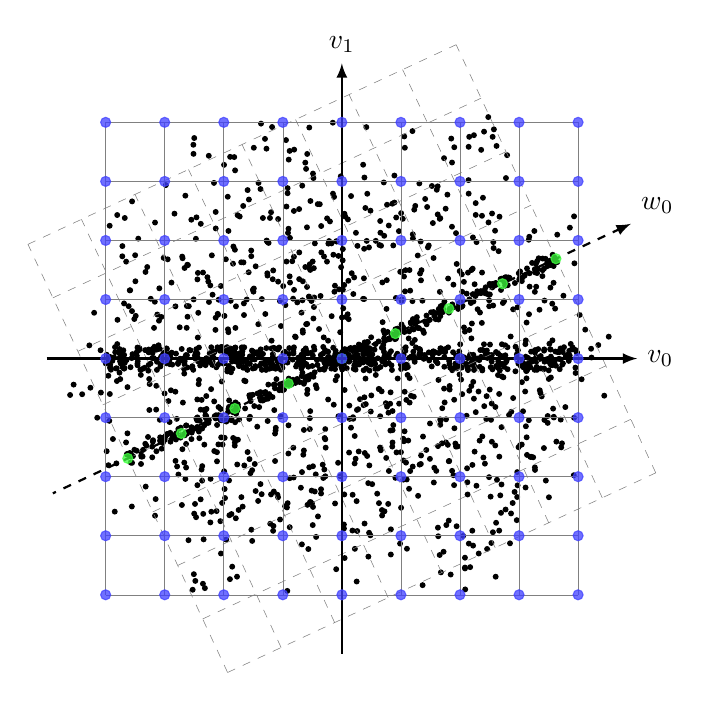
\begin{tikzpicture}[rotate=0,scale=0.75]
	% grid lines
	\def\xmin{-4}
	\def\ymin{-4}
	\def\xmax{4}
	\def\ymax{4}
	\def\xinc{1}
	\def\yinc{1}
	\pgfmathsetmacro{\xcentre}{(\xmax + \xmin) / 2}
	\pgfmathsetmacro{\ycentre}{(\ymax + \ymin) / 2}
	\pgfmathsetmacro{\xnext}{\xmin+\xinc}
	\pgfmathsetmacro{\ynext}{\ymin+\yinc}
	\def\angle{25}

	\def\xvar{3}
	\pgfmathsetmacro{\xvar}{(\xmax - \xmin)/2}
	\pgfmathsetmacro{\xoff}{0}
	\pgfmathsetmacro{\yvar}{\ymax/1.5}
	\pgfmathsetmacro{\yoff}{0}

	% draw random black dots all around
	\foreach \i in {1,2,...,250} {
		% ifthenelse can only compare integers
		\pgfmathsetmacro{\x}{(rand) * \xvar + \xoff}
		\pgfmathsetmacro{\y}{(rand) * \yvar + \yoff}
		\pgfmathtruncatemacro{\dist}{100*abs(\y-sin(\angle)/cos(\angle)*\x}
		\ifthenelse{\dist < 15}{\def\colour{black!40}}{\def\colour{black}}
		\filldraw [black] (\x,\y) circle (0.040);
	}

	\foreach \i in {1,2,...,250} {
		% ifthenelse can only compare integers
		\pgfmathsetmacro{\x}{(rand) * \xvar + \xoff}
		\pgfmathsetmacro{\y}{(rand) * \yvar + \yoff}
		\pgfmathsetmacro{\xrot}{\x*cos(\angle) - \y*sin(\angle)}
		\pgfmathsetmacro{\yrot}{\x*sin(\angle) + \y*cos(\angle)}
		\pgfmathtruncatemacro{\dist}{100*abs(\yrot-sin(\angle)/cos(\angle)*\xrot}
		\ifthenelse{\dist < 25}{\def\colour{black!40}}{\def\colour{black}}
		\filldraw [black] (\xrot,\yrot) circle (0.040);
	}

	\foreach \i in {1,2,...,250} {
		% ifthenelse can only compare integers
		\pgfmathsetmacro{\x}{(rand) * \xvar + \xoff}
		\pgfmathsetmacro{\y}{(rand) * \yvar + \yoff}
		\pgfmathsetmacro{\xrot}{\x*cos(-\angle) - \y*sin(-\angle)}
		\pgfmathsetmacro{\yrot}{\x*sin(-\angle) + \y*cos(-\angle)}
		\pgfmathtruncatemacro{\dist}{100*abs(\yrot-sin(\angle)/cos(\angle)*\xrot}
		\ifthenelse{\dist < 25}{\def\colour{black!40}}{\def\colour{black}}
		\filldraw [black] (\xrot,\yrot) circle (0.040);
	}

	\foreach \i in {1,2,...,250} {
		% ifthenelse can only compare integers
		\pgfmathsetmacro{\x}{(rand) * \xvar + \xoff}
		\pgfmathsetmacro{\y}{(rand) * \yvar + \yoff}
		\pgfmathsetmacro{\xrot}{\x*cos(90) - \y*sin(90)}
		\pgfmathsetmacro{\yrot}{\x*sin(90) + \y*cos(90)}
		\pgfmathtruncatemacro{\dist}{100*abs(\yrot-sin(\angle)/cos(\angle)*\xrot}
		\ifthenelse{\dist < 25}{\def\colour{black!40}}{\def\colour{black}}
		\filldraw [black] (\xrot,\yrot) circle (0.040);
	}

	% draw gray dots around main axis
	\pgfmathsetmacro{\yvar}{0.20}
	\foreach \i in {1,2,...,500} {
		% ifthenelse can only compare integers
		\pgfmathsetmacro{\x}{(rand) * \xvar + \xoff}
		\pgfmathsetmacro{\y}{(rand) * \yvar + \yoff}
		%\shade [ball color = black, opacity = 1] (\x,\y) circle (0.040);
		\filldraw [black] (\x,\y) circle (0.040);
	}

	% draw random red dots around secondary helper axis
	\draw[style=help lines, dashed, very thin, rotate=\angle] (\xmin,\ymin) grid (\xmax,\ymax);
	\draw[-latex,thick,dashed] (\xcentre,\ycentre) --++ (\angle:\xmax+1.4) node [above right]{$w_0$};
	\draw[thick,dashed,] (\xcentre,\ycentre) --++ (\angle:-\xmax-1.4);
	\pgfmathsetmacro{\yvar}{0.10}
	\foreach \i in {1,2,...,300} {
		\pgfmathsetmacro{\x}{(rand) * \xvar + \xoff}
		\pgfmathsetmacro{\y}{(rand) * \yvar + \yoff}
		\pgfmathsetmacro{\xrot}{\x*cos(\angle) - \y*sin(\angle)}
		\pgfmathsetmacro{\yrot}{\x*sin(\angle) + \y*cos(\angle)}
		\pgfmathsetmacro{\radius}{3}
		\pgfmathtruncatemacro{\smallcircle}{10 * (\x*\x + \y*\y) - \radius}
		\ifthenelse{\smallcircle < 0}{\def\colour{black}}{\def\colour{black!40}}
		\filldraw [black] (\xrot,\yrot) circle (0.040);
	}

	% draw axis for secondary helper transform
	\foreach \x in {\xmin,\xnext,...,\xmax} {
			\pgfmathsetmacro{\xrot}{\x*cos(\angle)}
			\pgfmathsetmacro{\yrot}{\x*sin(\angle)}
			\filldraw [green!75, opacity = 0.75] (\xrot,\yrot) circle (0.085);
	}

	\draw[style=help lines, very thin] (\xmin,\ymin) grid (\xmax,\ymax);
	% main axis
	\draw[-latex, thick] (\xmin-1,\ycentre) -- (\xmax+1,\ycentre) node[right] {$v_0$};
	\draw[-latex, thick] (\xcentre,\ymin-1) -- (\xcentre,\ymax+1) node[above] {$v_1$};
	\pgfmathsetseed{5}
	
	\foreach \x in {\xmin,\xnext,...,\xmax} {
		\foreach \y in {\ymin,\ynext,...,\ymax} {
			\filldraw [blue!75, opacity = 0.75] (\x,\y) circle (0.085);
		}
	}

\end{tikzpicture}
}
	{\includegraphics{./figures/it_diagram.pdf}}
	\caption[Illustration of the incomplete transform concepts]
	{Illustration of the incomplete transform concepts.
	An additional basis vector ($w_0$ is added to assist an orthogonal
	transform ($v_0,v_1$))}
	\label{fig:it_diagram}
\end{figure}

However, there exists a secondary direction that cannot be represented
compactly using the $(v_0,v_1)$ base vectors:
both axis are required to describe the coordinates of those points.
Just by adding an extra axis, $w_0$, adapted to this secondary direction, an
effective and sparser representation of those dots can be achieved.

Therefore, the dots plotted in this space can be efficiently represented thanks
to the union of two transforms.
One transform is complete, the second one, which can be conceived as a
complete transform, is restricted to only one base vector, the principal
component:
this way, the compactness is guaranteed, as only one transform coefficient
needs to be transmitted.

If only one adapted transform had been used in figure~\ref{fig:it_diagram}
to adapt to all those points, such as the \acl{KLT}, the main axis would have
been placed somewhere between $v_0$ and $w_0$.

\subsection{Complexity analysis}
\label{sub:it_complexity_analysis}

Incomplete transforms are proposed in this work to provide a low complexity
approach to the non-separable \ac{MDTC} systems.
A remarkable consequence of using incomplete transforms is a decrease in
complexity when decoding a signal, since there will be one coefficient
different from zero, decoding implies multiplying the base vector by the
transformed coefficient.

In image coding, a separable two-dimensional is expressed as
in~\eqref{eqn:sep_transform}.
Assuming the image is composed of $8\times8$ blocks, $\x$ stands for the
$8\times8$ pixels, and $\X$ their frequency representation.
$\A$ is the $8\times8$ 1D transform.
The usual transform used in image coding is the \ac{DCT}-II, whose fast
algorithm requires in the order of 12 multiplications and 29 additions per
$8\times1$ vector.
As $8$ vectors per block need to be processed both for the vertical and
horizontal transform, processing an $8\times8$ block requires a total of 192
multiplications and 464 additions.
This number of operations is identical for the inverse transform.

For an incomplete transform, only one axis needs to be processed:
each axis being formed by 64 values in this example.
Consequently, only 64 multiplications and 63 additions are also needed to
transform the input block $\x$ into the transform domain, that is, a simple
correlation of the first base vector with the block $\x$.
For the inverse transformation, only 64 multiplications are needed, since the
first and only transform coefficient multiplies the first basis vector to
recover the spatial domain samples.

As a result, in this case, the incomplete transforms can be applied with a
number of operations of approximately one third of the cost of the fastest
separable transforms.
This complexity reduction benefits both the encoder and the decoder.

It is also worth noticing that those incomplete transforms are chosen
non-separable and, therefore, able to exploit any linear correlation amongst
pixels within a block.

\section{Design of incomplete transforms}
\label{sec:it_design_of_incomplete_transforms}

The incomplete transform design is based upon the \ac{RDOT} model proposed
in~\cite{sezer-08-sparse-orthonormal-transforms} and detailed in
\S\ref{sec:rdot}.
The original method describes a way of iteratively deriving one optimal
transform for some given training data and an initial transform by using a
metric that includes a sparsity constraint.
This section adapts the learning method for incomplete transforms.

\subsection{Incomplete transform learning}
\label{sub:it_incomplete_transform_learning}

The learning phase of incomplete transforms uses the same method presented in
\S\ref{sec:rdot}, particularly in~\eqref{eqn:rdot-nsep}.
The design of an incomplete transform take one extra step apart from those
required in the \ac{RDOT} learning:
after the hard-thresholding of the coefficients, only the first coefficient is
kept.
Consequently, the $\ell_0$ norm of the transform coefficients is always equal
to one for any incomplete transform.
Therefore, for a given set of training signals, one obtains a transform
consisting of one meaningful base vector.
The remaining vectors, albeit constituting a complete transform with the first
base vector, are useless for the aim of the application.

For consistency with previous Chapters, the learning set consists of
prediction residuals issued from an \ac{HEVC} \ac{AI} coding for $8\times8$
blocks, the same one used in Chapters~\ref{cha:mddt} and~\ref{cha:mdtc}.

\subsubsection{Multiple incomplete transforms}
\label{ssub:it_multiple_incomplete_transforms}

In Chapter~\ref{cha:mdtc} the use of multiple transforms inside each \ac{IPM}
was introduced.
A decision was made to keep the default \ac{HEVC} transform in each \ac{TU}
size for compatibility reasons.
However, since incomplete transforms are designed with a strong sparsity
constraint on the quantised coefficients, a complete transform is needed to
guarantee that all signals can be expressed in the transform domain at a
chosen level of fidelity.
By using the same design as in the previous Chapter (one main transform plus
$2^N$ incomplete transforms), signals would be able to have a fall-back
transform when incomplete transforms do not provide the desired level of
fidelity in terms of distortion.

As a result, the learning algorithm for non-separable transforms has remained
almost untouched from algorithm~\ref{alg:clustering}, described in
\S\ref{sub:mdtc_learning_algorithm}, only the design of the transform has been
modified by just keeping the first coefficient after the hard-thresholding.
After that, residuals are evaluated using the \ac{RDOT} metric to assign them
to a particular transform.

To illustrate the effectiveness of the learning process,
figure~\ref{fig:it_num_zero} presents how an increase on the number of
incomplete transforms is able to provide a more sparse representation of
the signal in the transform domain.
This Illustration is based on the \ac{IPM} 6 for $8\times8$ blocks.

\begin{figure}[tp]
	\centering
	\ifthenelse{\usepdfs = 0}
	{\begin{tikzpicture}
	\pgfplotsset{/tikz/font={\footnotesize}}
	\begin{axis}[
			xlabel={number of incomplete transforms},
			%ylabel={overall ${\Vert\cdot\Vert}^2+\lambda{\Vert\cdot\Vert}_0$},
			grid=both,
			scale only axis,
			width=0.8\textwidth,
			height=0.2\textheight,
			%ytick={29, 29.5, ..., 32},
			y tick label style={
				/pgf/number format/.cd,
				fixed,
				fixed zerofill,
				precision=0,
				/tikz/.cd
			},
			%xmode=log,
			%log basis x={2},
			xtick={0, 1, 2, 4, 8, 16, 32},
			%xticklabels={0, 1, 2, 4, 8, 16, 32, 64},
			yticklabel=\pgfmathprintnumber{\tick}\,\%,
			xmin=0, xmax=32,
			ymin=60, ymax=100,
			%xmin=0.5, xmax=128,
			%ymin=29, ymax=32,
			%legend entries={DCT, DST, RDOT},
			%legend style={nodes=right},
			%legend pos= north east
		]

		\addplot[red, thick, mark=*] table {
		0		100
		1		92.2
		2		86
		4		81
		8		76.1
		16		70.4
		32		66.1
		};
	\end{axis}
\end{tikzpicture}
}
	{\includegraphics{./figures/it_num_zero_plot.pdf}}
	\caption{Percentage of non-zero coefficients referred to the \acs{DCT}}
	\label{fig:it_num_zero}
\end{figure}

To evaluate this, the average number of significant coefficients is computed
for different coding configurations (from 1 to 32 incomplete transforms used
in conjunction with the \ac{DCT}).
The results are presented relative to the reference system, which consists of
a coding system using the \ac{DCT} alone, such as the \ac{HEVC}.
As the number of incomplete transforms is increased, the proportion of
significant coefficients is decreased to 66\% of its original value for a
similar distortion:
this validates the fact that more sparse representations can be achieved with
the adjunction of incomplete transforms to the traditional \ac{DCT}.

The result of a learning experiment is shown in
figure~\ref{fig:it_32_transforms}, where 32 $8\times8$ incomplete transforms
are presented.
\begin{figure}[tp]
	\centering
	\includegraphics[width=0.8\linewidth]{./figures/it_32_transforms.png}
	\caption{List of 32 incomplete transforms for $8\times8$ blocks and
	\acs{IPM} 6}
	\label{fig:it_32_transforms}
\end{figure}
For each one, only the first base vector is displayed, since it is the only
one delivering significant transformed coefficients.
In the case of two-dimensional signals, such as images, incomplete transforms can
be directly interpreted as texture patterns against whom the input signal is
matched.
The learning set in this experiment is made of prediction residuals extracted
from a directional mode from the \ac{HEVC} coding scheme.
The selected mode (\ac{IPM} 6) corresponds to an angular prediction of
approximately $+\SI{26}{\degree}$.
Accordingly, the blocks selected by \ac{HEVC} for this mode mostly present a
directional pattern following that prediction.
It can be observed how the incomplete transforms have patterns containing that
particular direction, each exhibiting a particular band-shaped pattern.
Note that the \ac{DCT} requires a significant number of coefficients to
represent such directional, and inherently non-separable, patterns because
none of the \ac{DCT} bases expresses that direction.

\section{Incomplete transforms in video coding}
\label{sec:it_video_coding}

The usefulness of incomplete transforms has also been applied to \ac{HEVC}.
To evaluate the performance of the approach, a set of $4\times4$ and
$8\times8$ incomplete transforms is designed for each \ac{HEVC} \ac{IPM}.
At the encoder, for each block, the best \ac{IPM}/transform pair is selected,
exactly in the same way as the \ac{MDTC} system from Chapter~\ref{cha:mdtc}.

\subsection{Signalling of incomplete transforms in the bitstream}
\label{sub:it_signalling}

The signalling scheme for incomplete transforms is inherited from the
\ac{MDTC} system:
a flag indicates whether the default \ac{HEVC} transform is used.
If that is not the case a fixed length codeword indicates which incomplete
transform has been chosen by the encoder for that \ac{IPM}.

Incomplete transforms have a special feature that generic \acp{RDOT} used in
the \ac{MDTC} system do not have:
they always output a signal that has only one coefficient different from zero.
Consequently, the residual signal bitstream syntax can be reduced:
the significance map (i.e.\ the location of the significant coefficients) does
not need to be transmitted, since the position of the last element different
from zero is known when using incomplete transforms.
This fact can be taken advantage of by removing the
\texttt{last\_sig\_coeff\_x} and \texttt{last\_sig\_coeff\_y} prefix and
suffix syntax elements from the conveyed bitstream~\cite{JCTVC-G704}.

\subsection{Performances of different configurations}
\label{sub:it_performances}

Experiments have been performed following the common test conditions described
in~\cite{bossen-12-common-test-conditions} for the \ac{HEVC} test set.
Incomplete transforms have been enabled for $4\times4$ and $8\times8$
\acp{TU} in order to make the system comparable to the \ac{MDTC} systems from
the previous section.
In particular, 8 additional transforms have been designed for $4\times4$
\acp{TU} and 32 for $8\times8$ \acp{TU}.

The results of encoding the \ac{HEVC} test set using incomplete transforms are
detailed in table~\ref{tab:bd_rate_it}.
Performances are much lower than those presented in the previous Chapter for
the \ac{MDTC} system.
However, as explained in \S\ref{sub:it_coding_complexity} and
\S\ref{sub:it_storage_requirements}, incomplete transforms requirements are
also much lower than a \ac{MDTC} system.

When incomplete transforms are enabled only for $4\times4$ \acp{TU}, the
system presents modest performances (around 0.4\% of bit-rate savings) for
both \ac{AI} and \ac{RA} coding configurations.
The system starts presenting more substantial performances when enabling
incomplete transforms for $8\times8$ \acp{TU}, providing 1\% of average
bit-rate savings.
If incomplete transforms are enabled for both \ac{TU} sizes, the average
bit-rate savings achieve 1.4\% for the \ac{AI} coding configuration and 1\%
for \ac{RA}.

Sequences that performed exceptionally well using the \ac{MDTC} system due to
their non-separable nature, such as \emph{BasketballDrill} present bit-rate
savings of more that 8\% using this approach.

\begin{table}[tb]
	\centering
	\small
	\begin{tabularx}{\textwidth}{c|X|rr|rr|rr}
		\multicolumn{2}{c}{} &
		\multicolumn{2}{c|}{$4\times4$} &
		\multicolumn{2}{c|}{$8\times8$} &
		\multicolumn{2}{c}{$4\times4$ \& $8\times8$} \\
		\cline{2-8}
		\multicolumn{1}{c}{} & {Sequence} &
		\multicolumn{1}{c}{ \acs{AI}} & \multicolumn{1}{c|}{ \acs{RA}} &
		\multicolumn{1}{c}{ \acs{AI}} & \multicolumn{1}{c|}{ \acs{RA}} &
		\multicolumn{1}{c}{ \acs{AI}} & \multicolumn{1}{c}{ \acs{RA}} \\
		\hline
		\hline
		\multirow{5}{2cm}{\centering Class A ($2560\times1600$)}
		& NebutaFestival         &  0.01 &  0.00 &  0.00 & -0.04 &  0.01 & -0.03 \\
		& PeopleOnStreet         &  0.00 &  0.02 & -0.64 & -0.32 & -0.86 & -0.37 \\
		& SteamLocomotiveTrain   &  0.04 & -0.12 &  0.03 &  0.16 &  0.03 &  0.19 \\
		& Traffic                &  0.02 & -0.24 & -0.68 & -0.62 & -0.88 & -1.04 \\
		\cline{2-8} &
		Average                  &  0.02 & -0.08 & -0.32 & -0.20 & -0.43 & -0.31 \\
		\hline
		\hline
		\multirow{6}{2cm}{\centering Class B ($1920\times1080$)}
		& BasketballDrive        & -0.10 &  0.02 & -1.07 & -0.72 & -1.31 & -0.78 \\
		& BQTerrace              & -0.36 & -0.39 & -1.06 & -0.76 & -1.41 & -1.10 \\
		& Cactus                 & -0.18 & -0.32 & -1.38 & -0.87 & -1.73 & -1.25 \\
		& Kimono1                &  0.07 &  0.02 & -0.31 & -0.17 & -0.32 & -0.23 \\
		& ParkScene              &  0.13 &  0.08 & -0.15 & -0.16 & -0.19 & -0.24 \\
		\cline{2-8} &
		Average                  & -0.09 & -0.12 & -0.80 & -0.54 & -0.99 & -0.72 \\
		\hline
		\hline
		\multirow{5}{2cm}{\centering Class C ($832\times480$)}
		& BasketballDrill        & -3.21 & -1.95 & -6.22 & -2.91 & -8.22 & -4.35 \\
		& BQMall                 & -0.10 & -0.19 & -0.66 & -0.44 & -1.03 & -0.77 \\
		& PartyScene             & -0.10 & -0.29 & -0.18 & -0.15 & -0.40 & -0.54 \\
		& RaceHorses             & -0.31 & -0.23 & -0.44 & -0.37 & -0.85 & -0.51 \\
		\cline{2-8} &
		Average                  & -0.93 & -0.67 & -1.88 & -0.97 & -2.63 & -1.54 \\
		\hline
		\hline
		\multirow{5}{2cm}{\centering Class D ($416\times240$)}
		& BasketballPass         & -0.18 & -0.06 & -0.47 & -0.31 & -0.88 & -0.55 \\
		& BlowingBubbles         & -0.15 & -0.37 & -0.21 & -0.07 & -0.52 & -0.49 \\
		& BQSquare               & -0.32 & -0.37 & -0.25 & -0.19 & -0.59 & -0.51 \\
		& RaceHorses             & -0.37 & -0.09 & -0.32 & -0.12 & -0.86 & -0.37 \\
		\cline{2-8} &
		Average                  & -0.26 & -0.22 & -0.31 & -0.17 & -0.71 & -0.48 \\
		\hline
		\hline
		\multirow{4}{2cm}{\centering Class E ($1280\times720$)}
		& FourPeople             & -0.03 & -0.46 & -1.07 & -1.03 & -1.36 & -1.58 \\
		& Johnny                 & -0.13 & -0.75 & -1.25 & -1.16 & -1.56 & -1.84 \\
		& KristenAndSara         & -0.31 & -0.59 & -1.15 & -0.77 & -1.56 & -1.44 \\
		\cline{2-8} &
		Average                  & -0.16 & -0.60 & -1.16 & -0.99 & -1.49 & -1.62 \\
		\hline
		\hline
		\multirow{5}{2cm}{\centering Class F (various resolutions)}
		& BasketDrillText        & -2.54 & -1.67 & -4.83 & -2.33 & -6.49 & -3.66 \\
		& ChinaSpeed             & -0.40 & -0.29 & -0.45 & -0.26 & -0.90 & -0.61 \\
		& SlideEditing           & -0.23 & -0.24 & -0.51 & -0.61 & -0.71 & -0.81 \\
		& SlideShow              & -0.73 & -0.76 & -0.81 & -0.83 & -1.51 & -1.64 \\
		\cline{2-8} &
		Average                  & -0.97 & -0.74 & -1.65 & -1.01 & -2.40 & -1.68 \\
		\hline
		\hline
		All sequences &
		Overall                  & -0.40 & -0.38 & -1.00 & -0.63 & -1.42 & -1.02 \\
	\end{tabularx}
	\caption{Y \acs{BD}-rate (\%) for low complexity and high performance \acs{MDTC} systems}
	\label{tab:bd_rate_it}
\end{table}

\begin{figure}[tb]
	\centering
	\ifthenelse{\usepdfs = 0}
	{
\begin{tikzpicture}
	\pgfplotsset{/tikz/font={\small}}
	\begin{axis}[
		grid=both,
		width=1.0\textwidth,
		height=0.3\textheight,
		x tick label style={
		/pgf/number format/1000 sep=},
		ytick={0,-1,...,-9},
		y tick label style={
			/pgf/number format/.cd,
			fixed,
			fixed zerofill,
			precision=1,
		},
		y dir=reverse,
		ymax=0.5, ymin=-9,
		ylabel={Y BD-rate (\%)},
		% enlargelimits=0.15,
		enlarge y limits=false,
		enlarge x limits=0.04,
		legend style={at={(0.5,-0.40)},
		anchor=north,legend columns=-1},
		ybar,
		bar width=3pt,
		xtick=data,
		xtick align=inside,
		% nodes near coords,
		% xlabel={Sequences},
		% xlabel near ticks,
		symbolic x coords={
			NebutaFestival,
			PeopleOnStreet,
			SteamLocTrain,
			Traffic,
			BasketballDrive,
			BQTerrace,
			Cactus,
			Kimono1,
			ParkScene,
			BasketballDrill,
			BQMall,
			PartyScene,
			RaceHorses\_480p,
			BasketballPass,
			BlowingBubbles,
			BQSquare,
			RaceHorses\_240p,
			FourPeople,
			Johnny,
			KristenAndSara,
			BasketDrillText,
			ChinaSpeed,
			SlideEditing,
			SlideShow,
			Overall,
		},
		x tick label style={rotate=-60,anchor=west},
		]
		\addlegendentry{AI}
		\addplot coordinates {
		(NebutaFestival,   0.01)
		(PeopleOnStreet,  -0.86)
		(SteamLocTrain,    0.03)
		(Traffic,         -0.88)
		(BasketballDrive, -1.31)
		(BQTerrace,       -1.41)
		(Cactus,          -1.73)
		(Kimono1,         -0.32)
		(ParkScene,       -0.19)
		(BasketballDrill, -8.22)
		(BQMall,          -1.03)
		(PartyScene,      -0.40)
		(RaceHorses\_480p,-0.85)
		(BasketballPass,  -0.88)
		(BlowingBubbles,  -0.52)
		(BQSquare,        -0.59)
		(RaceHorses\_240p,-0.86)
		(FourPeople,      -1.36)
		(Johnny,          -1.56)
		(KristenAndSara,  -1.56)
		(BasketDrillText, -6.49)
		(ChinaSpeed,      -0.90)
		(SlideEditing,    -0.71)
		(SlideShow,       -1.51)
		(Overall,         -1.42)
		};

		\addlegendentry{RA}
		\addplot coordinates {
		(NebutaFestival,  -0.03)
		(PeopleOnStreet,  -0.37)
		(SteamLocTrain,    0.19)
		(Traffic,         -1.04)
		(BasketballDrive, -0.78)
		(BQTerrace,       -1.10)
		(Cactus,          -1.25)
		(Kimono1,         -0.23)
		(ParkScene,       -0.24)
		(BasketballDrill, -4.35)
		(BQMall,          -0.77)
		(PartyScene,      -0.54)
		(RaceHorses\_480p,-0.51)
		(BasketballPass,  -0.55)
		(BlowingBubbles,  -0.49)
		(BQSquare,        -0.51)
		(RaceHorses\_240p,-0.37)
		(FourPeople,      -1.58)
		(Johnny,          -1.84)
		(KristenAndSara,  -1.44)
		(BasketDrillText, -3.66)
		(ChinaSpeed,      -0.61)
		(SlideEditing,    -0.81)
		(SlideShow,       -1.64)
		(Overall,         -1.02)
		};

% 		\draw [thick] (35,0) --++ (0,900); % node [midway, sloped, above] {class A};
% 		\draw [thick] (85,0) --++ (0,900);
% 		\draw [thick] (125,0) --++ (0,900);
% 		\draw [thick] (165,0) --++ (0,900);
% 		\draw [thick] (195,0) --++ (0,900);
% 		\draw [thick] (235,0) --++ (0,900);

	\end{axis}
\end{tikzpicture}
}
	{\includegraphics{./figures/it_perf_4_8_plot.pdf}}
	\caption{\acs{BD}-rate for incomplete transforms enabled for $4\times4$
	and $8\times8$ \acsp{TU}}
	\label{fig:it_perf_4_8}
\end{figure}

Figure~\ref{fig:mdtc_bdrate_bdrill_inc_tr} shows the \ac{BD}-rate curves of
standard \ac{HEVC} and the \ac{MDTC} system using incomplete transforms on
$4\times4$ and $8\times8$ on the \emph{BasketballDrill} sequence.
The bit-rate savings are over 8\% and it can be seen that the system behaves
virtually in the same way as the \ac{MDTC} systems presented in the previous
Chapter for all bit-rate ranges.

\begin{figure}[tb]
	\centering
	\ifthenelse{\usepdfs = 0}
	{\begin{tikzpicture}

	\pgfplotsset{/tikz/font={\small}}
	\begin{axis}[
			xlabel={Bitrate (Mbps)},
			ylabel={PSNR (dB)},
			grid=both,
			scale only axis,
			width=0.9\textwidth,
			height=0.3\textheight,
			scaled x ticks = false,
			x tick label style={
				/pgf/number format/.cd,
				set thousands separator={\thinspace},
				/tikz/.cd
			},
			xtick={0,3,...,24},
			ytick={32,34,36,...,44},
			y tick label style={
				/pgf/number format/.cd,
				set decimal separator={.},
				fixed,
				fixed zerofill,
				precision=0,
				/tikz/.cd
			},
			xmin=0, xmax=21,
			ymin=32, ymax=44,
			% legend entries={HEVC,HEVC-MDTC},
			legend style={nodes=right},
			legend pos= south east
		]

		\addplot [mark=*,mark size=1pt, blue, thick, dashed] table {
		20.8089288	41.7621
		11.313408	38.3717
		6.0750904	35.4066
		3.3555608	32.7673
		};
		\addlegendentry{HEVC}

		\addplot [mark=*,mark size=1pt, red, thick] table {
		20.3708848	41.7809
		10.9011288	38.5696
		5.9389184	35.8291
		3.3554960	33.2623
		};
		\addlegendentry{HEVC-Inc.\ Tr.}

	\end{axis}
\end{tikzpicture}
}
	{\includegraphics{./figures/bdrate_bdrill_wvga_inc_tr_plot.pdf}}
	\caption[\acs{BD}-rate curves for incomplete transforms on
	\emph{BasketballDrill}]
	{\acs{BD}-rate curves of \emph{BasketballDrill} for the \acs{MDTC} system
	using incomplete transforms.
	This curve represents a bit-rate improvement of 8.22\% over \acs{HEVC}.}
	\label{fig:mdtc_bdrate_bdrill_inc_tr}
\end{figure}

\subsection{Coding complexity}
\label{sub:it_coding_complexity}

Despite using non-separable incomplete transforms, which are notably less
complex than regular non-separable and even separable transforms, the encoding
complexity is increased.
This is due to the fact that incomplete transforms are used as a simplified
\ac{MDTC} system, where many transforms are tested for a same block size.
This fact makes the encoder explore many coding possibilities that are
unavailable to \ac{HEVC}.
That being said, the increase in encoding complexity is lower than for a
full-fledged \ac{MDTC} system, since testing incomplete transforms is much
faster.

On the decoder side, the situation changes in favour of the incomplete
transforms with regards to \ac{HEVC}.
Since all coding choices are made by the encoder and the decoder only has to
apply the signalled transform, which as equal (if the \ac{DCT}/\ac{DST} is
chosen) or lower complexity, the decoding complexity is a bit lower that that
of \ac{HEVC}.

The actual results for encoding and decoding complexity are contained in
table~\ref{tab:it_complexity}.
The decoder presents complexities a bit lower than \ac{HEVC}.

\begin{table}[tb]
	\centering
	\small
	\begin{tabular}{l|r|r|r}
		& \multicolumn{1}{c|}{$4\times4$}
		& \multicolumn{1}{c|}{$8\times8$}
		& \multicolumn{1}{c}{$4\times4$ \& $8\times8$} \\
		\hline\hline
		Encoding & 210\% & 250\% & 340\% \\
		Decoding &  97\% &  99\% & 100\% \\
	\end{tabular}
	\caption{Relative average complexity of incomplete transform systems to
	\acs{HEVC}}
	\label{tab:it_complexity}
\end{table}


\subsection{Storage requirements}
\label{sub:it_storage_requirements}
\index{ROM}

Due to the similarities to the \ac{MDTC} system, the non-separable incomplete
transforms also need to be stored.
However, in this case, the storage requirements are divided by $N^2$, with $N$
being the \ac{TU} size for which the transforms are conceived, since only one
base vector is stored.
Assuming each transform coefficient is quantised to 1 byte and rounded to the
nearest integer, as in the \ac{MDDT} and \ac{MDTC} systems, this leads to
storage requirements of:
\begin{itemize}
	\item $4\times4$ transforms: \SI{16}{B} per transform.
	\item $8\times8$ transforms: \SI{64}{B} per transform.
\end{itemize}
For the system using 8 $4\times4$ transforms and 32 $8\times8$ transforms, the
global storage requirements are \SI{74.375}{\kilo B}, as there are 35
\acp{IPM}.

\section{Conclusions}
\label{sec:it_conclusions}

Incomplete transforms provide a simplified version of the \ac{MDTC} system,
presented in Chapter~\ref{cha:mdtc}.
These complementary transforms are able to increment the sparsity of the
signal in the transform domain:
the number of non-zero coefficients can been reduced to around two thirds of
its original value.

Experimental results on \ac{HEVC} prove that the sparsity improvements can
lead to bit-rate savings of around 1\% with peaks of up to 8\%, while keeping
the decoding complexity lower than that of \ac{HEVC}.
As a result, incomplete transforms provide an example of application for
non-separable transforms that can lead to bit-rate savings for reasonable
encoding complexity and storage amounts.
On the decoder side, incomplete transforms require less operations per block
than \ac{HEVC} transforms, leading to a decrease on the decoding complexity.

Summing up, \ac{MDTC} systems using incomplete transforms constitute a more
lightweight alternative to \ac{RDOT}-based \ac{MDTC} systems presented in
Chapter~\ref{cha:mdtc} that are able to provide improvements over \ac{HEVC}
across a wide range of bit-rate with low decoding complexity.

\chapter{Simplifications of \acs{MDTC} system for storage requirements}
\label{cha:real_world_system}
\chaptertoc

\section{Introduction}
\label{sec:rw_introduction}
\index{ROM}

Chapter~\ref{cha:mdtc} introduced the \acf{MDTC} system for video coding.
Significant bit-rate savings were obtained with regards to \ac{HEVC},
especially when using the non-separable high-performance system, where many
non-separable transforms were provided in each \ac{IPM}:
up to 7\% on average for the \ac{AI} coding configuration.

This chapter will take a look at different approaches to simplify the
system presented in Chapter~\ref{cha:mdtc} in terms of storage requirements
while trying to have minimum impact on its bit-rate savings.

\subsection{Discarding non-separable transforms}
\label{sub:discarding_non_separable_transforms}

In order to conceive a low complexity system that makes use of transform
competition, some concessions are required.
This Chapter proposes simplifications to the areas leading to significant
complexity increases in \ac{MDTC} systems, especially, to the storage
requirements.

The first approach for simplification is to suppress the use of non-separable
transforms, even though they provide notably better performances than their
separable counterparts, as seen in Chapters~\ref{cha:mddt} and~\ref{cha:mdtc}.
Non-separable transforms can definitively not accommodate a system with
neither storage restrictions, nor coding complexity limitations.
For this reason, this Chapter will only consider systems composed by separable
transforms.
As a consequence of ditching non-separable transforms, the average bit-rate
savings achievable on the \ac{HEVC} using separable high performance \ac{MDTC}
systems are around 4\%, which will be used as a reference when comparing the
simplified systems.

Furthermore, separable transform present increases of around 5\% in decoding
complexity, instead of the 20\% added by non-separable transforms.

\section{Source of the learning set}
\label{sec:rw_source_of_the_learning_set}

\subsection{Completely independent sets}
\label{sub:rw_completely_independent_sets}

A criticism that could be made to systems presented in
Chapters~\ref{cha:mddt},~\ref{cha:mdtc} and~\ref{cha:incomplete_transforms} is
that the testing set includes the learning set:
classes B and C have served as the learning set and the resulting transforms
to build the \ac{MDDT} and \ac{MDTC} systems have been tested against those
classes.
That being said, performances on classes not included in the learning set (A,
D, E and F) have similar levels of performances as described previously on
their respective system tables (see tables~\ref{tab:detailed_mddt_bd_rate},
\ref{tab:bd_rate_mdtc} and~\ref{tab:bd_rate_it}).

To remove any doubt about the effect of the learning data set, a completely
independent data set has been chosen and used to learn transforms.
In order to make all results available and reproducible, the sequence of
choice from which residuals have been output is \emph{Tears of Steel}, a
Creative Commons short film~\cite{blender-tearsofsteel}.
The film features computed generated imagery and unique a resolution of
$1920\times800$ at a frame rate of \SI{24}{\hertz} and a length of
\SI{12}{\minute} and \SI{14}{\second}.
Although it is composed of more that 130 sub-sequences, all of them share the
same video post-processing, frame rate, resolution, making a source of
residuals less heterogeneous than classes B and C from the \ac{HEVC} test set,
but providing a larger number of residuals (around as twice as many, in
total):
\begin{itemize}
	\item $4\times4$ residuals: over 142 million.
	\item $8\times8$ residuals: over 343 million.
\end{itemize}

The resulting transforms have served to build new \ac{MDTC} systems that have
been compared to the previous ones on different sequence sets.

Additionally, another independent set of sequences has been used to test the
performances of both learning sets (classes B and C, and \emph{Tears of
Steel}).
This set consists of 59 sequences at different resolutions ($1920\times1080$,
$1280\times720$, $832\times480$) and various frame rates (25, 30, 50, 60, 100,
120, 240 frames per second).
Each sequence has been limited to 5 frames, since all the tests are performed
in the \ac{AI} configuration.

From now on, the different sets will be referred to as:
\begin{itemize}
	\item BC: classes B and C from the \ac{HEVC} test set, used as the
		learning set in previous Chapters.
	\item ADEF: classes A, D, E and F from the \ac{HEVC} test set.
	\item 59seq: 5 frames of 59 heterogeneous (private) sequences for testing.
	\item ToS: the \emph{Tears of Steel} publicly available short film.
\end{itemize}

\subsection{Impact on the coding performances over the learning sets}
\label{sub:rw_performances_new_data_set}

This section presents the results of different \ac{MDTC} systems learnt with
BC and ToS, and then tested against BC, ADEF, 59seq and ToS.

The resulting systems performances are contained in
tables~\ref{tab:residuals_independence_4}
and~\ref{tab:residuals_independence_8} for $4\times4$ and $8\times8$ separable
transforms, respectively.
The table headers read as follows: Test set | Learning set.
The value before the pipe sign corresponds to the set of sequences that have
been tested and the value after the pipe to the learning set that has been
used.
Moreover, since the ToS learning set provides more residuals, more transforms
have been learnt for the $8\times8$ blocks.
Bit-rate savings are present for all transform configurations from both
residuals sources on all test sets, and they coherently increase with the
number of transforms.

\begin{table}[tb]
	\centering
	\small
	\begin{tabularx}{\linewidth}{r|cc|cc|cc|cc}
		\# tr. & BC | BC & BC | ToS & ADEF | BC & ADEF | ToS & 59seq | BC &
		59seq | ToS & ToS | BC & ToS | ToS \\
		\hline\hline
		1  & -0.69 & -0.61 & -0.85 & -0.95 & -0.48 & -0.48 & -0.13 & -0.17 \\
		2  & -0.93 & -0.85 & -1.16 & -1.21 & -0.66 & -0.66 & -0.21 & -0.25 \\
		4  & -1.08 & -1.05 & -1.32 & -1.54 & -0.76 & -0.80 & -0.23 & -0.31 \\
		8  & -1.23 & -1.14 & -1.48 & -1.68 & -0.86 & -0.91 & -0.27 & -0.34 \\
		16 & -1.28 & -1.22 & -1.65 & -1.85 & -0.93 & -0.96 & -0.30 & -0.34 \\
		32 & -1.28 & -1.25 & -1.76 & -1.89 & -0.93 & -0.99 & -0.27 & -0.35 \\
	\end{tabularx}
	\caption{\acs{BD}-rate (\%) for different testing and learning sets for
	$4\times4$ blocks}
	\label{tab:residuals_independence_4}
\end{table}

\begin{table}[tb]
	\centering
	\small
	\begin{tabularx}{\linewidth}{r|cc|cc|cc|cc}
		\# tr. & BC | BC & BC | ToS & ADEF | BC & ADEF | ToS & 59seq | BC &
		59seq | ToS & ToS | BC & ToS | ToS \\
		\hline\hline
		1   & -0.97 & -0.68 & -0.82 & -0.74 & -0.93 & -0.83 & -0.75 & -1.00 \\
		2   & -1.43 & -1.11 & -1.20 & -1.13 & -1.38 & -1.32 & -1.01 & -1.33 \\
		4   & -1.91 & -1.44 & -1.55 & -1.47 & -1.84 & -1.70 & -1.30 & -1.59 \\
		8   & -2.35 & -1.81 & -1.91 & -1.83 & -2.15 & -2.08 & -1.48 & -1.84 \\
		16  & -2.81 & -2.19 & -2.27 & -2.12 & -2.50 & -2.46 & -1.69 & -2.05 \\
		32  & -3.32 & -2.51 & -2.63 & -2.43 & -2.84 & -2.76 & -1.84 & -2.17 \\
		64  & -3.88 & -2.79 & -3.01 & -2.66 & -3.10 & -3.04 & -1.93 & -2.28 \\
		128 & ---   & -3.07 & ---   & -2.92 & ---   & -3.30 & ---   & -2.38 \\
	\end{tabularx}
	\caption{\acs{BD}-rate (\%) for different testing and learning sets for
	$8\times8$ blocks}
	\label{tab:residuals_independence_8}
\end{table}

To better understand the impact of the learning set on the different test
sets, figure~\ref{fig:residuals_independence} shows the results from
tables~\ref{tab:residuals_independence_4}
and~\ref{tab:residuals_independence_8}.
For the $4\times4$ case, there are few differences in performances between
both learning sets, BC and ToS.
Only classes ADEF (in blue) present some preference for the Tears of
Steel data set.
For the $8\times8$ case, there seems to be some over-learning for the
sequences used during the learning phase (BC and ToS), since they present
notable differences in performances when using their own learning set.
The rest of test sets present similar performance levels for both learning
sets.

\begin{figure}[tb]
	\centering
	\subfloat[Additional $4\times4$ transforms]
	{\ifthenelse{\usepdfs = 0}
	{\definecolor{greenish}{RGB}{0,145,0}
\begin{tikzpicture}
	\pgfplotsset{/tikz/font={\footnotesize}}
	\begin{axis}[
			xlabel={Additional $4\times4$ transforms},
			ylabel={Y BD-rate (\%)},
			grid=both,
			scale only axis,
			width=0.8\textwidth,
			height=0.3\textheight,
			xtick={0, 1, 2, 4, 8, 16, 32},
			x tick label style={
				/pgf/number format/.cd,
				fixed,
				fixed zerofill,
				precision=0,
			},
			y tick label style={
				/pgf/number format/.cd,
				fixed,
				fixed zerofill,
				precision=1,
			},
			ytick={0,-0.2,...,-4},
			xmin=0, xmax=32,
			ymin=-2.0, ymax=0,
			legend style={nodes=right},
			legend pos= north east,
		]

		\addplot [mark=*,mark size=1pt, red, thick] table {
		0	0
		1	-0.69
		2	-0.93
		4	-1.08
		8	-1.23
		16	-1.28
		32  -1.28
		};
		\addlegendentry{BC | BC}

		\addplot [mark=*,mark size=1pt, red, thick, dashed] table {
		0	0
		1	-0.61
		2	-0.85
		4	-1.05
		8	-1.14
		16	-1.22
		32  -1.25
		};
		\addlegendentry{BC | ToS}

		\addplot [mark=*,mark size=1pt, blue, thick] table {
		0	0
		1	-0.85
		2	-1.16
		4	-1.32
		8	-1.48
		16	-1.65
		32  -1.76
		};
		\addlegendentry{ADEF | BC}

		\addplot [mark=*,mark size=1pt, blue, thick, dashed] table {
		0	0
		1	-0.95
		2	-1.21
		4	-1.54
		8	-1.68
		16	-1.85
		32  -1.89
		};
		\addlegendentry{ADEF | ToS}

		\addplot [mark=*,mark size=1pt, greenish, thick] table {
		0	0
		1	-0.48
		2	-0.67
		4	-0.78
		8	-0.87
		16	-0.94
		32  -0.95
		};
		\addlegendentry{59seq | BC}

		\addplot [mark=*,mark size=1pt, greenish, thick, dashed] table {
		0	0
		1	-0.49
		2	-0.67
		4	-0.82
		8	-0.93
		16	-0.98
		32  -1.01
		};
		\addlegendentry{59seq | ToS}

		\addplot [mark=*,mark size=1pt, black, thick] table {
		0	0
		1	-0.13
		2	-0.21
		4	-0.23
		8	-0.27
		16	-0.30
		32  -0.27
		};
		\addlegendentry{ToS | BC}

		\addplot [mark=*,mark size=1pt, black, thick, dashed] table {
		0	0
		1	-0.17
		2	-0.25
		4	-0.31
		8	-0.34
		16	-0.34
		32  -0.35
		};
		\addlegendentry{ToS | ToS}

	\end{axis}
\end{tikzpicture}

% vim:set filetype=tex:
}
	{\includegraphics{./figures/residuals_independence_4_plot.pdf}}}
	\\
	\subfloat[Additional $8\times8$ transforms]
	{\ifthenelse{\usepdfs = 0}
	{\definecolor{greenish}{RGB}{0,145,0}
\begin{tikzpicture}
	\pgfplotsset{/tikz/font={\small}}
	\begin{axis}[
			% xlabel={Additional $8\times8$ transforms},
			ylabel={Y BD-rate (\%)},
			grid=both,
			scale only axis,
			width=0.9\textwidth,
			height=0.2\textheight,
			x tick label style={
				/pgf/number format/.cd,
				fixed,
				fixed zerofill,
				precision=0,
			},
			y tick label style={
				/pgf/number format/.cd,
				fixed,
				fixed zerofill,
				precision=1,
			},
			xtick={0,1,2,4,8,16,32,64,128},
			ytick={0,-0.5,...,-4},
			xmin=0, xmax=64,
			ymin=-4.0, ymax=0,
			legend style={nodes=right},
			legend pos= north east,
		]

		\addplot [mark=*,mark size=1pt, red, thick] table {
		0	0
		1	-0.97
		2	-1.43
		4	-1.91
		8	-2.35
		16	-2.81
		32  -3.32
		64	-3.88
		};
		\addlegendentry{BC | BC}

		\addplot [mark=*,mark size=1pt, red, thick, dashed] table {
		0	0
		1	-0.68
		2	-1.11
		4	-1.44
		8	-1.81
		16	-2.19
		32  -2.51
		64	-2.79
		};
		% 128	-3.07
		\addlegendentry{BC | ToS}

		\addplot [mark=*,mark size=1pt, blue, thick] table {
		0	0
		1	-0.82
		2	-1.20
		4	-1.55
		8	-1.91
		16	-2.27
		32  -2.63
		64	-3.01
		};
		\addlegendentry{ADEF | BC}

		\addplot [mark=*,mark size=1pt, blue, thick, dashed] table {
		0	0
		1	-0.74
		2	-1.13
		4	-1.47
		8	-1.83
		16	-2.12
		32  -2.43
		64	-2.66
		};
		% 128	-2.92
		\addlegendentry{ADEF | ToS}

		\addplot [mark=*,mark size=1pt, greenish, thick] table {
		0	0
		1	-0.94
		2	-1.40
		4	-1.86
		8	-2.18
		16	-2.54
		32  -2.88
		64	-3.14
		};
		\addlegendentry{59seq | BC}

		\addplot [mark=*,mark size=1pt, greenish, thick, dashed] table {
		0	0
		1	-0.84
		2	-1.33
		4	-1.72
		8	-2.10
		16	-2.48
		32  -2.79
		64	-3.07
		};
		% 128	-3.33
		\addlegendentry{59seq | ToS}

		\addplot [mark=*,mark size=1pt, black, thick] table {
		0	0
		1	-0.75
		2	-1.01
		4	-1.30
		8	-1.48
		16	-1.69
		32  -1.84
		64	-1.93
		};
		\addlegendentry{ToS | BC}

		\addplot [mark=*,mark size=1pt, black, thick, dashed] table {
		0	0
		1	-1.00
		2	-1.33
		4	-1.59
		8	-1.84
		16	-2.05
		32  -2.17
		64	-2.28
		};
		% 128	-2.38
		\addlegendentry{ToS | ToS}

	\end{axis}
\end{tikzpicture}
}
	{\includegraphics{./figures/residuals_independence_8_plot.pdf}}}
	\\
	\caption{\acs{BD}-rate for different testing and learning sets}
	\label{fig:residuals_independence}
\end{figure}

This comes as a reassuring fact, since the residuals from ToS have less
variability in terms of camera filters, frame rate, resolution and have even
synthetic images, whereas the rest of sequences are exclusively composed of
natural images coming from different sources at different frame rates and
resolutions.

Table~\ref{tab:cross_bdrate_learn} illustrates the impact of changing the
learning set to design the high performance \ac{MDTC} system: losses of 0.4
and 0.2 are observed for the \ac{AI} and \ac{RA} configurations, respectively
for the \ac{HEVC} test set, which means that the new reference \ac{MDTC}
system has bit-rate savings of 3.65\% on the \ac{HEVC} test set, instead of
4.10\%.

\begin{table}[tb]
	\centering
	\small
	\begin{tabular}{c|cc|c}
		& \multicolumn{2}{c|}{\acs{HEVC} test set} & 59seq \\
		\diagbox{Learn}{Test}
		& \acs{AI} & \acs{RA} & \acs{AI} \\
		\hline\hline
		BC  & -4.10\% & -2.76\% & -3.54\% \\
		ToS & -3.65\% & -2.62\% & -3.36\% \\
	\end{tabular}
	\caption{Bit-rate savings for separable high performance \acs{MDTC} using
	different test sets}
	\label{tab:cross_bdrate_learn}
\end{table}

Finally, as the 59seq set will be serving as the new reference system, against
which new improvements will be measured, the separable high performance
\ac{MDTC} system (16 additional transforms for $4\times4$ \acp{TU} and 32 for
$8\times8$ \acp{TU}) has been evaluated on this test set.
The results are also presented in table~\ref{tab:cross_bdrate_learn}.
Performances of the high performance \ac{MDTC} system are almost equivalent on
the 59seq testing set, independently of the used learning set.

In this section, it has been proved that the transforms learnt and tested in
previous Chapters were subject to some over-learning, leading to slightly
better performances than when using a learning set completely independent from
the test set.
This over-learning reassures the fact that the designed transforms are able to
adapt to the learning set, while showing that there is little dependence to
the learning set.
It can be concluded that changing the learning set does not affect
the overall performance:
the order of improvement is learning set independent although some small local
differences appear.

\section{Non-homogeneous \acs{MDTC} systems}
\label{sec:non_homogeneous_mdtc_systems}

In Chapter~\ref{cha:mdtc}, the \ac{MDTC} system was introduced.
The \ac{MDTC} system was presented as an evolved \ac{MDDT} system, in which,
instead of only one transform, a fixed number of transforms was provided
inside each \ac{IPM}.
However, as exemplified in figure~\ref{fig:hevc_ipm_usage}, \ac{HEVC} does not
use all \acp{IPM} equally:
\ac{HEVC} favours the signalling of the \acp{IPM} that are most often used
during the encoding of a sequence in terms of signalling.
This technique is named \acp{MPM} and it is explained in detail
in~\cite{wien-15-hevc}.
As a result, it might be counter productive to add a high number of transforms
to those modes that are hardly chosen, making them even less cost efficient,
since the extra transforms need to be signalled, as well.
Using a different number of transforms inside each \ac{IPM} does not require
any additional signalling to the transform index, since the encoder will know
how many transforms are available for each \ac{IPM}.

\begin{figure}[tb]
	\centering
	\ifthenelse{\usepdfs = 0}
	{\begin{tikzpicture}
	\pgfplotsset{/tikz/font={\small}}
	\begin{axis}[
		grid=both,
		width=1.0\textwidth,
		height=0.3\textheight,
		ytick={0,200,...,1400},
		y tick label style={
		/pgf/number format/.cd,
		fixed,
		fixed zerofill,
		precision=0,
		set thousands separator={\thinspace}},
		% y dir=reverse,
		ymax=1400, ymin=0,
		ylabel={Number of blocks ($\times1000$)},
		% enlargelimits=0.15,
		enlarge y limits=false,
		enlarge x limits=0.04,
		legend style={at={(0.5,-0.15)},
		anchor=north,legend columns=-1},
		ybar interval,
		% bar width=2pt,
		% bar shift=10pt
		xtick=data,
		xtick align=inside,
		% nodes near coords,
		% xlabel={Sequences},
		% xlabel near ticks,
		% x tick label style={rotate=-60,anchor=west},
		]
		\addlegendentry{$4\times4$}
		\addplot coordinates { % values have beed divided by 1000
		(0, 1364.213)
		(1,  724.842)
		(2,   56.522)
		(3,   61.151)
		(4,   55.249)
		(5,   64.906)
		(6,   98.925)
		(7,  122.995)
		(8,  273.925)
		(9,  416.868)
		(10, 726.798)
		(11, 731.229)
		(12, 286.635)
		(13, 248.812)
		(14, 307.531)
		(15, 214.435)
		(16, 152.227)
		(17, 162.321)
		(18,  71.355)
		(19, 107.414)
		(20,  91.012)
		(21,  98.337)
		(22, 126.187)
		(23, 128.947)
		(24, 149.842)
		(25, 307.650)
		(26, 738.189)
		(27, 276.359)
		(28, 150.686)
		(29, 116.680)
		(30, 105.906)
		(31,  75.812)
		(32,  72.256)
		(33,  75.184)
		(34,  53.216)
		(35, 0)
		};

		\addlegendentry{$8\times8$}
		\addplot coordinates { % values have beed divided by 1000
		(0, 1215.199)
		(1,  689.480)
		(2,   81.395)
		(3,   29.846)
		(4,   33.355)
		(5,   42.454)
		(6,   57.356)
		(7,   75.645)
		(8,  151.422)
		(9,  331.490)
		(10, 426.614)
		(11, 428.937)
		(12, 159.159)
		(13, 149.122)
		(14, 128.801)
		(15,  90.122)
		(16,  58.692)
		(17,  40.322)
		(18, 109.448)
		(19,  27.579)
		(20,  33.682)
		(21,  44.409)
		(22,  49.680)
		(23,  63.084)
		(24,  86.251)
		(25, 239.589)
		(26, 540.578)
		(27, 217.064)
		(28,  89.107)
		(29,  66.923)
		(30,  50.982)
		(31,  43.990)
		(32,  37.089)
		(33,  32.193)
		(34,  72.435)
		(35,0)
		};
	\end{axis}
\end{tikzpicture}
}
	{\includegraphics{./figures/ipm_hist_bdrill_qp22_4_8_plot.pdf}}
	\caption[\acs{IPM} usage in \acs{HEVC}]
	{\acs{IPM} usage in \acs{HEVC} on \emph{BasketballDrive} for \acs{QP} 22}
	\label{fig:hevc_ipm_usage}
\end{figure}

Consequently, next Section proposes a systematic way of generating \ac{MDTC}
systems taking into account the storage requirements.
Since the \acs{ROM} required to store the transforms is directly related to
the number of transforms, and the number of transforms to the encoding
complexity, by limiting the amount of \acs{ROM}, the system might also
simplified in terms of encoding time.

This section proposes a gradient descent algorithm to generate \ac{MDTC} with
\acs{ROM} constraints and a non-homogeneous number of transforms in its
\acp{IPM}.

\subsection{Preparation phase}
\label{sub:rw_preparation_phase}

In order to build a system with a different number of transforms in each
\ac{IPM}, additional transforms for $4\times4$ and $8\times8$ \acp{TU} have
been learnt.
For the $4\times4$ \ac{TU}, up to 32 additional transforms are available, and
up to 128 for $8\times8$ \ac{TU}.

As a reference point, tables~\ref{tab:homogeneous_mdtc_4}
and~\ref{tab:homogeneous_mdtc_8} contain different separable homogeneous
\ac{MDTC} systems using $4\times4$ and $8\times8$ transforms, respectively.
Systems have been labelled using the following convention: {4tN--8tM}.
Where 4 and 8 stand for the transform sizes, t for the type, in this case s,
meaning separable transforms, and N and M represent the number of additional
transforms added in each \ac{IPM} for the respective transform size.
Each system has information about its \acs{ROM} requirements, the bit-rate
savings and the encoding complexity with regards \ac{HEVC}.
Consistent bit-rate savings are observed when increasing the number of
transforms for both \ac{TU} sizes, even if the $4\times4$ transform
performances seem to saturate with 16 and 32 additional transforms.

\begin{table}[tb]
	\centering
	\begin{tabular}{r|r|r|r}
	System & \multicolumn{1}{c|}{\acs{ROM}} & Y \acs{BD}-rate & Complexity \\
	\hline\hline
	 4s1--8s0 &  \SI{1.64}{\kilo B} & -0.49\% & 127\% \\
	 4s2--8s0 &  \SI{3.28}{\kilo B} & -0.67\% & 141\% \\
	 4s4--8s0 &  \SI{6.56}{\kilo B} & -0.82\% & 167\% \\
	 4s8--8s0 & \SI{13.13}{\kilo B} & -0.93\% & 219\% \\
	4s16--8s0 & \SI{26.25}{\kilo B} & -0.98\% & 322\% \\
	4s32--8s0 & \SI{52.50}{\kilo B} & -1.01\% & 527\% \\
	\end{tabular}
	\caption{Summary of $4\times4$ homogeneous \acs{MDTC} systems learnt with
	ToS on 59seq}
	\label{tab:homogeneous_mdtc_4}
\end{table}

\begin{table}[tb]
	\centering
	\begin{tabular}{r|r|r|r}
	System & \multicolumn{1}{c|}{\acs{ROM}} & Y \acs{BD}-rate & Complexity \\
	\hline\hline
	  4s0--8s1 &   \SI{6.56}{\kilo B} & -0.84\% &  127\% \\
	  4s0--8s2 &  \SI{13.13}{\kilo B} & -1.33\% &  142\% \\
	  4s0--8s4 &  \SI{26.25}{\kilo B} & -1.72\% &  171\% \\
	  4s0--8s8 &  \SI{52.50}{\kilo B} & -2.10\% &  229\% \\
	 4s0--8s16 & \SI{105.00}{\kilo B} & -2.48\% &  345\% \\
	 4s0--8s32 & \SI{210.00}{\kilo B} & -2.79\% &  577\% \\
	 4s0--8s64 & \SI{420.00}{\kilo B} & -3.07\% & 1041\% \\
	4s0--8s128 & \SI{840.00}{\kilo B} & -3.33\% & 1970\% \\
	\end{tabular}
	\caption{Summary of $8\times8$ homogeneous \acs{MDTC} systems learnt with
	ToS on 59seq}
	\label{tab:homogeneous_mdtc_8}
\end{table}

\subsection{Determination of number of transforms per \acs{IPM}}
\label{sub:rw_determination_number_transforms_ipm}

In order to improve current homogeneous \ac{MDTC} systems in the \acs{ROM} ---
Y \acs{BD}-rate plane plane, algorithm~\ref{alg:vmdtc_iter} presents a
systematic way of designing a non-homogeneous \ac{MDTC} system, using a
gradient approach.
The algorithm starts with an unmodified version of \ac{HEVC}.
Then, it encodes the 59seq test set enabling one transform by \ac{IPM} at a
time.
After that, it chooses the \ac{IPM} providing the best \acs{BD}-rate/\acs{ROM}
trade-off.
That configuration is then used as the new base system and the transforms are
doubled each time for the \ac{IPM} that gives the best ratio.

\begin{algorithm}
	\small
	\SetKwData{encode}{encode}
	\SetKwData{computeBestRatio}{computeBestRatio}
	\SetKwInOut{Input}{testSet}
	\SetKwInOut{Output}{nTransf[35]}
	\Input{59seq}
	\Output{0}
	\BlankLine%
	\BlankLine%
	tmpTransf[35]: 0
	\BlankLine%
	/* Initial encoding of the test set using HEVC */
	\BlankLine%
	\encode(nTransf, testSet)
	\BlankLine%
	\While{1}
	{
		/* increment the transforms per IPM */
		\BlankLine%
		\For{$i=0$ \KwTo{} $34$}
		{
			\eIf{nTransf[i] == 0}
			{
				tmpTransf[i] = 1
			}
			{
				tmpTransf[i] = 2 * nTransf[i]
			}
		}
		\BlankLine%
		/* encode the test set using the 35 configurations */
		\BlankLine%
		results = \encode(tmpTransf, testSet)
		\BlankLine%
		/* find the IPM providing the best BD-rate/ROM ratio */
		\BlankLine%
		bestIPM = \computeBestRatio(results)
		\BlankLine%
		/* update the transform configuration */
		\BlankLine%
		nTransf[bestIPM] = tmpTransf[bestIPM]
	}
	\caption{Iterative non-homogeneous \acs{MDTC} design}
	\label{alg:vmdtc_iter}
\end{algorithm}

Figure~\ref{fig:vmdtc_iter} displays different \ac{MDTC} systems on the
\acs{ROM} --- Y \ac{BD}-rate plane.
The main systems that are compared are the homogeneous and non-homogeneous
(issued from the iterative algorithm) systems using $4\times4$ and $8\times8$
transforms.
Each point in this figure requires encoding 59 sequences at 4 \acp{QP} for
each one of the 35 \acp{IPM}, leading to a total of \num{8260} encodings.

Systems that combine both transform sizes are also presented in the figure.
Iterative non-homogeneous \ac{MDTC} systems have more flexibility in terms of
the number of transforms enabled in each \ac{IPM} and, therefore, in their
storage requirements.
For this reason, iterative systems provide a lot more granularity than
homogeneous ones, allowing for better \acs{ROM}--\ac{BD}-rate trade-offs
and more selectable \acs{ROM} operating points.

Red lines in figure~\ref{fig:vmdtc_iter} represent the $4\times4$ only
\ac{MDTC} systems.
Homogeneous $4\times4$ systems start saturating in terms of bit-rate savings
after adding 8 additional transform in each \ac{IPM}.
The non-homogeneous $4\times4$ system is able to achieve the same performances
as the homogeneous system, with less \acs{ROM}.

The interest of the non-homogeneous systems is clearer when using $8\times8$
transforms (blue lines), since the storage requirements are higher.
In this case, almost a factor of two can be observed in terms of \acs{ROM} for
the same \ac{BD}-rate in homogeneous and non-homogeneous systems.
Moreover, it can be noticed that, for the $8\times8$ systems, the bit-rate
savings are proportional, in a logarithmic scale, to the \acs{ROM}
requirements and, consequently, to the number of transforms.

\begin{figure}[tb]
	\centering
	\ifthenelse{\usepdfs = 0}
	{\definecolor{greenish}{RGB}{0,145,0}
\begin{tikzpicture}
	\pgfplotsset{/tikz/font={\footnotesize}}
	\begin{axis}[
			% title=Bitrate savings: $-8.94\%$. SNR improvement: $0.46$ dB,
			xlabel={ROM (kB)},
			ylabel={Y BD-rate (\%)},
			grid=both,
			scale only axis,
			width=0.8\textwidth,
			height=0.3\textheight,
			xtick={0.25,0.5,1,2,4,8,16,32,64,128,256,512,1024},
			xticklabels={0.25,0.5,1,2,4,8,16,32,64,128,256,512,1024},
			% x tick label style={
			% 	/pgf/number format/.cd,
			% 	fixed,
			% 	fixed zerofill,
			% 	precision=0,
			% },
			% scaled x ticks=false,
			ytick={0,-0.5,...,-4},
			y tick label style={
				/pgf/number format/.cd,
				fixed,
				fixed zerofill,
				precision=1,
				/tikz/.cd
			},
			xmode=log,
			log basis x=2,
			xmin=0.25, xmax=1024,
			ymin=-4.0, ymax=0,
			legend style={nodes=right},
			legend pos= south west
		]

		\addlegendentry{$4\times4$ iterations}
		\pgfplotstableread{figures/vmdtc_iter_4.dat}\table
		\addplot[red, thick, mark=*, mark size=0.5pt, smooth]
		table[x=rom,y=bdrate,col sep=tab] from \table;

		\addlegendentry{$8\times8$ iterations}
		\pgfplotstableread{figures/vmdtc_iter_8.dat}\table
		\addplot[blue, thick, mark=*, mark size=0.5pt, smooth]
		table[x=rom,y=bdrate,col sep=tab] from \table;

		\addlegendentry{$4\times4$ sep. hom. MDTC}
		\addplot [only marks, mark=x,mark size=2pt, red, thick, 
		visualization depends on=\thisrow{alignment} \as \alignment,
		nodes near coords, % Place nodes near each coordinate
		point meta=explicit symbolic, % The meta data used in the nodes is not explicitly provided and not numeric
		every node near coord/.style={anchor=\alignment} % Align each coordinate at the anchor 40 degrees clockwise from the right edge
		] table [meta index=2] {
		rom	dtt_bdrate	dtt_label	alignment
		1.64	-0.49	\tiny{\color{black}4s1--8s0}	-90
		3.28	-0.67	\tiny{\color{black}4s2--8s0}	-90
		6.56	-0.82	\tiny{\color{black}4s4--8s0}	-90
		13.13	-0.93	\tiny{\color{black}4s8--8s0}	-90
		26.25	-0.98	\tiny{\color{black}4s16--8s0}	-90
		52.2	-1.01	\tiny{\color{black}4s32--8s0}	-90
		};

		\addlegendentry{$8\times8$ sep. hom. MDTC}
		\addplot [only marks, mark=x,mark size=2pt, blue, thick, 
		visualization depends on=\thisrow{alignment} \as \alignment,
		nodes near coords, % Place nodes near each coordinate
		point meta=explicit symbolic, % The meta data used in the nodes is not explicitly provided and not numeric
		every node near coord/.style={anchor=\alignment} % Align each coordinate at the anchor 40 degrees clockwise from the right edge
		] table [meta index=2] {
		rom	dtt_bdrate	dtt_label	alignment
		6.56	-0.84	\tiny{\color{black}4s0--8s1}	90
		13.13	-1.33	\tiny{\color{black}4s0--8s2}	-90
		26.25	-1.72	\tiny{\color{black}4s0--8s4}	-90
		52.50	-2.10	\tiny{\color{black}4s0--8s8}	-90
		105.00	-2.48	\tiny{\color{black}4s0--8s16}	-90
		210.00	-2.79	\tiny{\color{black}4s0--8s32}	-90
		420.00	-3.07	\tiny{\color{black}4s0--8s64}	-90
		840.00	-3.33	\tiny{\color{black}4s0--8s128}	-60
		};

		\addlegendentry{Comb. sep. hom. MDTC}
		\addplot [only marks, mark=x,mark size=2pt, greenish, thick,
		visualization depends on=\thisrow{alignment} \as \alignment,
		nodes near coords, % Place nodes near each coordinate
		point meta=explicit symbolic, % The meta data used in the nodes is not explicitly provided and not numeric
		every node near coord/.style={anchor=\alignment} % Align each coordinate at the anchor 40 degrees clockwise from the right edge
		] table [meta index=2] {
		rom	dtt_bdrate	dtt_label	alignment
		8.20	-1.38	\tiny{\color{black}4s1--8s1}	180
		14.77	-1.80	\tiny{\color{black}4s1--8s2}	180
		16.41	-1.97	\tiny{\color{black}4s2--8s2}	180
		27.89	-2.14	\tiny{\color{black}4s1--8s4}	180
		32.81	-2.45	\tiny{\color{black}4s4--8s4}	180
		59.06	-2.76	\tiny{\color{black}4s4--8s8}	180
		65.62	-2.83	\tiny{\color{black}4s8--8s8}	180
		118.12	-3.15	\tiny{\color{black}4s8--8s16}	180
		223.12	-3.39	\tiny{\color{black}4s8--8s32}	-90
		236.25	-3.44	\tiny{\color{black}4s16--8s32}	90
		};

		\addlegendentry{Comb. sep. het. MDTC}
		\addplot [only marks, mark=o,mark size=1pt, greenish, thick,
		visualization depends on=\thisrow{alignment} \as \alignment,
		nodes near coords, % Place nodes near each coordinate
		point meta=explicit symbolic, % The meta data used in the nodes is not explicitly provided and not numeric
		every node near coord/.style={anchor=\alignment} % Align each coordinate at the anchor 40 degrees clockwise from the right edge
		] table [meta index=2] {
		rom	dtt_bdrate	dtt_label	alignment
		0.98	-0.74 \tiny{\color{black}1 kB}	0
		1.97	-1.02 \tiny{\color{black}2 kB}	0
		3.98	-1.39 \tiny{\color{black}4 kB}	0
		7.97	-1.82 \tiny{\color{black}8 kB}	0
		12.00	-2.10 \tiny{\color{black}12 kB}	0
		15.61	-2.22 \tiny{\color{black}16 kB}	0
		23.95	-2.52 \tiny{\color{black}24 kB}	0
		31.78	-2.68 \tiny{\color{black}32 kB}	0
		47.39	-2.85 \tiny{\color{black}48 kB}	0
		63.89	-3.00 \tiny{\color{black}64 kB}	0
		95.53	-3.27 \tiny{\color{black}96 kB}	0
		127.41	-3.41 \tiny{\color{black}128 kB}	0
		};

\end{axis}
\end{tikzpicture}
}
	{\includegraphics{./figures/vmdtc_iter_plot.pdf}}
	\caption{Different \acs{MDTC} systems on the \acs{ROM} --- Y \acs{BD}-rate
	plane}
	\label{fig:vmdtc_iter}
\end{figure}

Finally, some interesting configurations have been built combining $4\times4$
and $8\times8$ systems, in both homogeneous and non-homogeneous ways,
represented using green lines.
Again, for these systems, especially on low \acs{ROM} configurations, a factor
of two in terms of storage requirements is observed.
Each one of the points from the learnt systems has two coordinates: \acs{ROM}
and \ac{BD}-rate.

This means that, for a given \acs{ROM} constraint, one can find the
combination of the $4\times4$ and $8\times8$ systems that offers the best
trade-off in terms of storage requirements and bit-rate savings.
Consequently, the optimal combinations of non-homogeneous \ac{MDTC} systems
have been found by setting a \acs{ROM} specification and selecting the
combination of heterogeneous $4\times4$ and $8\times8$ systems that provide
the best \ac{BD}-rate without exceeding the specified \acs{ROM}.
The results of all systems combination can be found in the scatter plot of
figure~\ref{fig:vmdtc_combined}.
It can bee seen that the points present a lower boundary, which corresponds to
the best combinations for a given \acs{ROM}.

\begin{figure}[tb]
	\centering
	\ifthenelse{\usepdfs = 0}
	{\definecolor{greenish}{RGB}{0,145,0}
\begin{tikzpicture}
	\pgfplotsset{/tikz/font={\footnotesize}}
	\begin{axis}[
			% title=Bitrate savings: $-8.94\%$. SNR improvement: $0.46$ dB,
			xlabel={ROM (kB)},
			ylabel={Y BD-rate (\%)},
			grid=both,
			scale only axis,
			width=0.8\textwidth,
			height=0.3\textheight,
			xtick={0.25,0.5,1,2,4,8,16,32,64,128,256,512,1024},
			xticklabels={0.25,0.5,1,2,4,8,16,32,64,128,256,512,1024},
			% x tick label style={
			% 	/pgf/number format/.cd,
			% 	fixed,
			% 	fixed zerofill,
			% 	precision=0,
			% },
			% scaled x ticks=false,
			ytick={0,-0.5,...,-4},
			y tick label style={
				/pgf/number format/.cd,
				fixed,
				fixed zerofill,
				precision=1,
				/tikz/.cd
			},
			xmode=log,
			log basis x=2,
			xmin=0.25, xmax=256,
			ymin=-4.0, ymax=0,
			legend style={nodes=right},
			legend pos= north east
		]

		% \addlegendentry{Combinations of $4\times4$ and $8\times8$
		% heterogeneous systems}
		\pgfplotstableread{figures/vmdtc_systems_combined.dat}\table
		\addplot[only marks, mark=*, mark size=0.5pt, red]
		table[x=rom,y=bdrate,col sep=tab] from \table;

\end{axis}
\end{tikzpicture}
}
	{\includegraphics{./figures/vmdtc_systems_combined_plot.pdf}}
	\caption[All possible combinations of $4\times4$ and $8\times8$
	non-homogeneous systems]
	{All possible combinations of $4\times4$ and $8\times8$
	non-homogeneous systems based on independent selection of the appropriate
	number of $4\times4$ and $8\times8$ transforms.
	The lower boundary shows the hypothetical bit-rate savings that could be
	obtained if there were no penalty when combining independently designed
	$4\times4$ and $8\times8$ transforms.}
	\label{fig:vmdtc_combined}
\end{figure}

The selected \acs{ROM} requirements for the systems presented in
figure~\ref{fig:vmdtc_iter} are detailed in
table~\ref{tab:non_hom_mdtc}.
Information about their actual \acs{ROM} requirements, \ac{BD}-rate and
encoding complexity are provided.
There are some remarkable points, such as the system at \SI{8}{\kilo B},
which can achieve bit-rate savings of 1.8\% with an encoding complexity
slightly higher than twice of \ac{HEVC}'s.
Another interesting point is the \SI{64}{\kilo B} system, being able to
provide bit-rate savings of 3\% at roughly seven times the complexity of
\ac{HEVC}.

\begin{table}[tb]
	\centering
	\small
	\begin{tabular}{r|r|r|r}
	System & \multicolumn{1}{c|}{\acs{ROM}} & Y \acs{BD}-rate & Complexity \\
	\hline\hline
	  \SI{1}{\kilo B} &   \SI{0.98}{\kilo B} & -0.74\% & 122\% \\
	  \SI{2}{\kilo B} &   \SI{1.97}{\kilo B} & -1.02\% & 131\% \\
	  \SI{4}{\kilo B} &   \SI{3.98}{\kilo B} & -1.39\% & 157\% \\
	  \SI{8}{\kilo B} &   \SI{7.97}{\kilo B} & -1.82\% & 200\% \\
	 \SI{12}{\kilo B} &  \SI{12.00}{\kilo B} & -2.10\% & 221\% \\
	 \SI{16}{\kilo B} &  \SI{15.61}{\kilo B} & -2.22\% & 245\% \\
	 \SI{24}{\kilo B} &  \SI{23.95}{\kilo B} & -2.52\% & 345\% \\
	 \SI{32}{\kilo B} &  \SI{31.78}{\kilo B} & -2.68\% & 387\% \\
	 \SI{48}{\kilo B} &  \SI{47.39}{\kilo B} & -2.85\% & 520\% \\
	 \SI{64}{\kilo B} &  \SI{63.89}{\kilo B} & -3.00\% & 660\% \\
	 \SI{96}{\kilo B} &  \SI{95.53}{\kilo B} & -3.27\% & 851\% \\
	\SI{128}{\kilo B} & \SI{127.41}{\kilo B} & -3.41\% & 931\% \\
	\end{tabular}
	\caption{Non-homogeneous \acs{MDTC} systems with \acs{ROM} constraints}
	\label{tab:non_hom_mdtc}
\end{table}

Nonetheless, learning the $4\times4$ and $8\times8$ non-homogeneous \ac{MDTC}
systems independently and then combining them to design the complete system is
a suboptimal approach.
The suboptimality can be spotted by comparing figures~\ref{fig:vmdtc_iter}
and~\ref{fig:vmdtc_combined}:
the lower boundary of figure~\ref{fig:vmdtc_combined} is lower than the actual
measurements from figure~\ref{fig:vmdtc_iter}.
This is due to the fact that, when combining both transform sizes, there is an
overlap between them in the coded blocks, making the performances of the
combined $4\times4$ and $8\times8$ systems to be a bit lower than the sum of
the corresponding separate systems.

Moreover, presented iterated \ac{MDTC} systems have only the choice to use 1
to 32 additional transforms for $4\times4$ \acs{TU} and 1 to 128 for
$8\times8$ \acp{TU}.
This is another source of suboptimality once the maximum number of transforms
has been enabled in one \ac{IPM}, since the system lacks the choice to double
the number of transforms for that \ac{IPM}.

As a final observation, non-homogeneous systems learnt iteratively with
\acs{ROM} constraints present a pattern in the number of transforms enabled in
each \ac{IPM}.
Those \acp{IPM} that are most used in \ac{HEVC} (0, 1, 10 and 26) tend to make
use of a higher number of transforms than the rest of them, which matches
closely the \ac{IPM} use in \ac{HEVC} from figure~\ref{fig:hevc_ipm_usage}:
systems tend to use more transforms on \acsp{IPM} 0, 1, 10, 26 and around
them.
A detailed table breaking down each \ac{MDTC} system listed in
table~\ref{tab:non_hom_mdtc} is presented in
appendix~\ref{cha:transform_usage_in_mdtc_systems}, particularly
tables~\ref{tab:config_nonsym_mdtc_4} and~\ref{tab:config_nonsym_mdtc_8}, for
$4\times4$ and $8\times8$ \acp{TU}, respectively.

\section{Symmetrical \acs{MDTC} systems}
\label{sec:sym_mdtc}

\subsection{Further simplifications taking advantage of \acs{IPM} symmetries}
\label{sub:further_simplifications_taking_advantage_of_ipm_symmetries}

In order to reduce the \acs{ROM} impact of the transforms, one can take
advantage of geometrical symmetries existing amongst \ac{HEVC} \acp{IPM}:
within the 35 \acp{IPM} in \ac{HEVC}, symmetries in prediction residuals can
be observed for directional modes (\acp{IPM} from 2 to 34).
Figure~\ref{fig:sym_pred_directions} contains a simplified version of the
\ac{HEVC} \acp{IPM} which illustrates the proposed symmetrical relations.

\begin{figure}[t]
	\centering
	\ifthenelse{\usepdfs = 0}
	{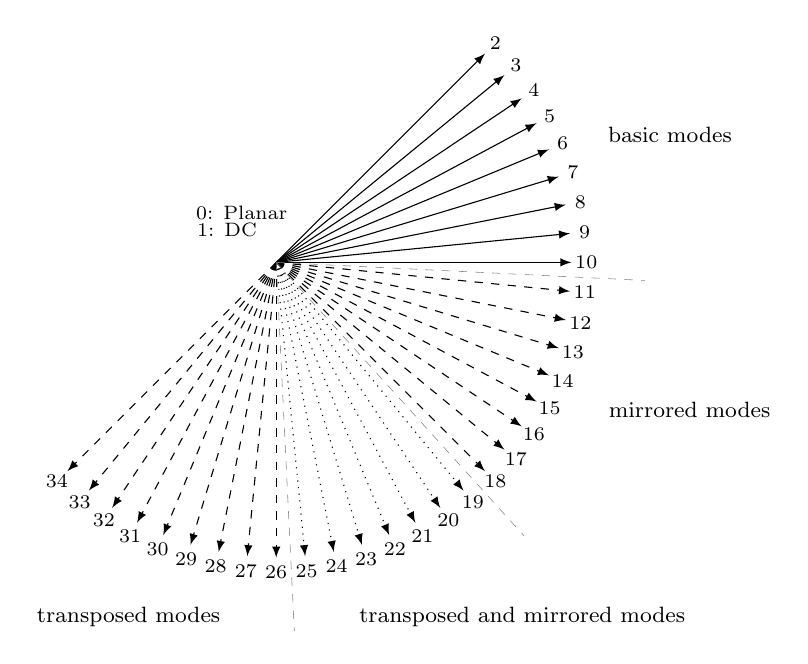
\begin{tikzpicture}[scale=1.25]

	\def\startx{0}
	\def\starty{0}
	\def\radius{3.0}
	\def\startangle{45}
	\def\colour{black}
	\def\style{}

	\draw (-0.35, 0.5) node {\scriptsize 0: \color{\colour}{Planar}};
	\draw (-0.50, 0.5) node[below] {\scriptsize 1: \color{\colour}{DC}};

	% draw the basic HEVC IPMs with different styles
	\foreach \direction in {2,3,...,34}
	{%
		% set the angle of current prediction direction 
		\pgfmathsetmacro{\angle}{\startangle - (\direction - 2) * 180 / 32}
		% \ifthenelse{\direction = 18}{\def\thickness{very thick}};
		% \ifthenelse{\direction = 26}{\def\thickness{very thick}};
		% basic modes
		\ifthenelse{\direction > 1 \AND \direction < 11}{\def\colour{black}};
		% mirror modes
		\ifthenelse{\direction > 10 \AND \direction < 19}{\def\style{dashed}};
		% transposed and mirrored modes
		\ifthenelse{\direction > 18 \AND \direction < 26}{\def\style{dotted}};
		% transposed modes
		\ifthenelse{\direction > 25 \AND \direction < 35}{\def\style{dashed}};
		% draw the directions
		\draw[-latex,\colour, \style] (\startx,\starty) --++ (\angle:\radius);
		% label each prediction direction
		\draw(\angle:\radius + 0.15) node {\scriptsize \direction};
	}

	% draw separators
	\foreach \direction in {10, 18, 25}
	{
		\pgfmathsetmacro{\angle}{\startangle - (\direction + 0.5 - 2) * 180 / 32}
		\draw[help lines, dashed] (\startx,\starty) --++ (\angle:\radius + 0.75);
	}

	% label IPM groups
	\draw (4,1.3) node {\footnotesize basic modes};
	\draw (4.2,-1.5) node {\footnotesize mirrored modes};
	\draw (2.5,-3.6) node {\footnotesize transposed and mirrored modes};
	\draw (-1.5,-3.6) node {\footnotesize transposed modes};

\end{tikzpicture}

% vim:set filetype=tex:
}
	{\includegraphics{./figures/sym-pred-directions.pdf}}
	\caption{The 35 \acsp{IPM} in \acs{HEVC} and their symmetries}
	\label{fig:sym_pred_directions}
\end{figure}

It can be stated that residuals issued from the first half (2--17) are closely
related to the transposed version of the second half (19--34).
Figure~\ref{fig:symmetry_transposed} illustrates the average $4\times4$
residuals profile and how the first half of the directional \acp{IPM} relates
to the second one.

\begin{figure}[tb]
	\centering
	\def\scalefactor{0.125}
	\small
	\npdigits{4}{0}
	\foreach \direction in {2,3,4,5,6,7,8,9,10,11,12,13,14,15,16,17}
	{
		\def\size{4}
		\numprint{\direction}
		\includegraphics[scale=\scalefactor]{./figures/residuals_profile_\size x\size/residuals-\size x\size-\direction.png}
		%
		\pgfmathtruncatemacro{\directiont}{36-\direction}
		\numprint{\directiont}
		\includegraphics[scale=\scalefactor]{./figures/residuals_profile_\size x\size/residuals-\size x\size-\directiont.png}
		%
		\numprint{\directiont}$^T$
		\reflectbox{               % mirror +
		\rotatebox[origin=c]{-90}{ % rotation = transposition
		\includegraphics[scale=\scalefactor]{./figures/residuals_profile_\size x\size/residuals-\size x\size-\directiont.png}
		}}
		\hfill
		\def\size{8}
		\numprint{\direction}
		\includegraphics[scale=\scalefactor]{./figures/residuals_profile_\size x\size/residuals-\size x\size-\direction.png}
		%
		\pgfmathtruncatemacro{\directiont}{36-\direction}
		\numprint{\directiont}
		\includegraphics[scale=\scalefactor]{./figures/residuals_profile_\size x\size/residuals-\size x\size-\directiont.png}
		%
		\numprint{\directiont}$^T$
		\reflectbox{               % mirror +
		\rotatebox[origin=c]{-90}{ % rotation = transposition
		\includegraphics[scale=\scalefactor]{./figures/residuals_profile_\size x\size/residuals-\size x\size-\directiont.png}
		}}
		\par
	}
	\caption{Average $4\times4$ and $8\times8$ residual profiles showing the
	symmetries around \acs{IPM} 18}
	\label{fig:symmetry_transposed}
\end{figure}

These symmetries can be taken one step beyond and be applied inside the first
half.
Although it might seem at first counter-intuitive, this decision can be
justified geometrically:
around \ac{IPM} 10, which is purely horizontal, it seems natural to think that
residuals from \ac{IPM} 9 (slightly diagonal up) and \ac{IPM} 11 (slightly
diagonal down) can be related via a horizontal mirroring operation
(top-bottom) or reflection.
Since the second half is related to the first half transposed, this property
applies around \ac{IPM} 26 in a similar fashion, through a vertical mirroring
(left-right).
Figures~\ref{fig:symmetry_transposed_mirror_4}
and~\ref{fig:symmetry_transposed_mirror_8} contain illustrative examples of
average profiles and they relations using these imposed symmetries.

\begin{figure}[tb]
	\centering
	\begin{minipage}{0.6\textwidth}
	\def\size{4}
	\def\scalefactor{0.125}
	\small
	\foreach \direction in {2}
	{
	    \numprint{\direction}
	    \includegraphics[scale=\scalefactor]{./figures/residuals_profile_\size x\size/residuals-\size x\size-\direction.png}
		%
		\pgfmathtruncatemacro{\directiont}{36-\direction}
		$\quad\directiont^T$
		\reflectbox{               % mirror +
		\rotatebox[origin=c]{-90}{ % rotation = transposition
		\includegraphics[scale=\scalefactor]{./figures/residuals_profile_\size x\size/residuals-\size x\size-\directiont.png}
		}}
		\pgfmathtruncatemacro{\directionm}{20-\direction}
		%
		\pgfmathtruncatemacro{\directiontm}{52-\directiont}
		$\quad\curvearrowupdown\directionm$
		\raisebox{\depth}{\scalebox{1}[-1]{ % vertical mirror
		\includegraphics[scale=\scalefactor]{./figures/residuals_profile_\size x\size/residuals-\size x\size-\directionm.png}
		}}
		\par
	}
	\foreach \direction in {3,4,5,6,7,8,9}
	{
	    $\direction$
	    \includegraphics[scale=\scalefactor]{./figures/residuals_profile_\size x\size/residuals-\size x\size-\direction.png}
		%
		\pgfmathtruncatemacro{\directiont}{36-\direction}
		$\quad\directiont^T$
		\reflectbox{               % mirror +
		\rotatebox[origin=c]{-90}{ % rotation = transposition
		\includegraphics[scale=\scalefactor]{./figures/residuals_profile_\size x\size/residuals-\size x\size-\directiont.png}
		}}
		%
		\pgfmathtruncatemacro{\directionm}{20-\direction}
		\pgfmathtruncatemacro{\directiontm}{52-\directiont}
		$\quad\curvearrowupdown\directionm$
		\raisebox{\depth}{\scalebox{1}[-1]{ % vertical mirror
		\includegraphics[scale=\scalefactor]{./figures/residuals_profile_\size x\size/residuals-\size x\size-\directionm.png}
		}}
		%
		\pgfmathtruncatemacro{\directiontm}{52-\directiont}
		$\quad\curvearrowupdown\directiontm^T$ % rotation 90 = transposition + mirror
		\includegraphics[scale=\scalefactor,angle=90]{./figures/residuals_profile_\size x\size/residuals-\size x\size-\directiontm.png}
		\par
}
\end{minipage}
	\caption[Average $4\times4$ residual profiles showing imposed symmetries]
	{Average $4\times4$ residual profiles showing imposed symmetries with
	transposition and vertical mirroring}
	\label{fig:symmetry_transposed_mirror_4}
\end{figure}

\begin{figure}[tb]
	\centering
	\begin{minipage}{0.6\textwidth}
	\def\size{8}
	\def\scalefactor{0.125}
	\small
	\foreach \direction in {2}
	{
	    \numprint{\direction}
	    \includegraphics[scale=\scalefactor]{./figures/residuals_profile_\size x\size/residuals-\size x\size-\direction.png}
		%
		\pgfmathtruncatemacro{\directiont}{36-\direction}
		$\quad\directiont^T$
		\reflectbox{               % mirror +
		\rotatebox[origin=c]{-90}{ % rotation = transposition
		\includegraphics[scale=\scalefactor]{./figures/residuals_profile_\size x\size/residuals-\size x\size-\directiont.png}
		}}
		\pgfmathtruncatemacro{\directionm}{20-\direction}
		%
		\pgfmathtruncatemacro{\directiontm}{52-\directiont}
		$\quad\curvearrowupdown\directionm$
		\raisebox{\depth}{\scalebox{1}[-1]{ % vertical mirror
		\includegraphics[scale=\scalefactor]{./figures/residuals_profile_\size x\size/residuals-\size x\size-\directionm.png}
		}}
		\par
	}
	\foreach \direction in {3,4,5,6,7,8,9}
	{
	    $\direction$
	    \includegraphics[scale=\scalefactor]{./figures/residuals_profile_\size x\size/residuals-\size x\size-\direction.png}
		%
		\pgfmathtruncatemacro{\directiont}{36-\direction}
		$\quad\directiont^T$
		\reflectbox{               % mirror +
		\rotatebox[origin=c]{-90}{ % rotation = transposition
		\includegraphics[scale=\scalefactor]{./figures/residuals_profile_\size x\size/residuals-\size x\size-\directiont.png}
		}}
		%
		\pgfmathtruncatemacro{\directionm}{20-\direction}
		\pgfmathtruncatemacro{\directiontm}{52-\directiont}
		$\quad\curvearrowupdown\directionm$
		\raisebox{\depth}{\scalebox{1}[-1]{ % vertical mirror
		\includegraphics[scale=\scalefactor]{./figures/residuals_profile_\size x\size/residuals-\size x\size-\directionm.png}
		}}
		%
		\pgfmathtruncatemacro{\directiontm}{52-\directiont}
		$\quad\curvearrowupdown\directiontm^T$ % rotation 90 = transposition + mirror
		\includegraphics[scale=\scalefactor,angle=90]{./figures/residuals_profile_\size x\size/residuals-\size x\size-\directiontm.png}
		\par
}
\end{minipage}
	\caption[Average $8\times8$ residual profiles showing imposed symmetries]
	{Average $8\times8$ residual profiles showing imposed symmetries with
	transposition and horizontal mirroring}
	\label{fig:symmetry_transposed_mirror_8}
\end{figure}

When both symmetries are exploited, the number of transforms of an \ac{MDTC}
system is no longer affected by a factor of 35 (the number of \acp{IPM}), but
by a factor of 11 (the number of basic \acp{IPM}), as presented in
table~\ref{tab:relations_ipm_residuals}.

\begin{table}[tb]
	\centering
	\small
	\begin{tabular}{c|ccc}
	\bf IPM &
	${(\cdot)}^T$ &
	\bf $\curvearrowupdown(\cdot)$ &
	\bf $\curvearrowupdown{(\cdot)}^T$ \\[1ex]
	\hline\hline
	\bf 0       & ---           & ---    & ---    \\
	\bf 1       & ---           & ---    & ---    \\
	\bf 2       & 34            & 18     & ---    \\
	\bf 3       & 33            & 17     & 19     \\
	\bf 4       & 32            & 16     & 20     \\
	\bf 5       & 31            & 15     & 21     \\
	\bf 6       & 30            & 14     & 22     \\
	\bf 7       & 29            & 13     & 23     \\
	\bf 8       & 28            & 12     & 24     \\
	\bf 9       & 27            & 11     & 25     \\
	\bf 10      & 26            & ---    & ---    \\
	\end{tabular}
	\caption{Symmetrical relations among \ac{IPM} residuals}
	\label{tab:relations_ipm_residuals}
\end{table}

Using these symmetries between \acp{IPM} implies manipulating the residual
before the transform stage.
This residual manipulation comes at no cost in terms of mathematical
operations, since it consists in pixel reordering.
Before transmitting a residual, the encoder will consider the following cases,
depending on the \ac{IPM}:
\begin{equation}
	\X =
	\begin{cases}
		\A \, \x & \;\;\, 0 \le \ac{IPM} \le 10 \\
		\A \, \curvearrowupdown\x & 11 \le \ac{IPM} \le 18 \\
		\A \, \curvearrowupdown\x^T & 19 \le \ac{IPM} \le 25 \\
		\A \, \x^T & 26 \le \ac{IPM} \le 34 \\
	\end{cases}
\end{equation}
Where $\A$ is a transform designed for the basic IPM set, $\x$ is the current
residual and $\curvearrowupdown$ represents the horizontal mirroring operator
(top-bottom).
Mirroring and transposing operations are used to make residuals compatible
with the transforms learnt for the basic IPM set.
These operations are only different ways of re-arranging the residual pixels
in a consistent way, which come at no computational cost.

\subsection{Symmetries performances on video coding}
\label{sub:symmetries_performances_on_video_coding}

Tables~\ref{tab:sym4} and~\ref{tab:sym8} show the impact of symmetries on
$4\times4$ and $8\times8$ \ac{MDTC} systems, respectively in the \acs{ROM} and
\ac{BD}-rate plane.
As demonstrated before, for the full-symmetrical \ac{MDTC} systems, \acs{ROM}
is decreased to around one third of its original value.
Bit-rate savings also experiment some losses, tending to decrease as the
number of transforms increases, since symmetrical system are more constrained
than non-symmetrical systems.
The encoding complexity for symmetrical system is equivalent to the one for
non-symmetrical ones, detailed in tables~\ref{tab:homogeneous_mdtc_4}
and~\ref{tab:homogeneous_mdtc_8}, since the number of transforms par \ac{IPM}
remains unchanged.

\begin{table}[tb]
	\centering
	\small
	\begin{tabular}{c|rr|rr}
		& \multicolumn{2}{c|}{non-symmetrical}
		& \multicolumn{2}{c}{symmetrical} \\
		\# tr & \multicolumn{1}{c}{\acs{ROM}} &
		\multicolumn{1}{c|}{Y \acs{BD}-rate} &
		\multicolumn{1}{c}{\acs{ROM}} &
		\multicolumn{1}{c}{Y \acs{BD}-rate} \\
		\hline \hline
		 1 &  \SI{1.64}{\kilo B} & -0.49\% &  \SI{0.52}{\kilo B} & -0.50\% \\
		 2 &  \SI{3.28}{\kilo B} & -0.67\% &  \SI{1.03}{\kilo B} & -0.63\% \\
		 4 &  \SI{6.56}{\kilo B} & -0.82\% &  \SI{2.06}{\kilo B} & -0.72\% \\
		 8 & \SI{13.13}{\kilo B} & -0.93\% &  \SI{4.13}{\kilo B} & -0.84\% \\
		16 & \SI{26.25}{\kilo B} & -0.98\% &  \SI{8.25}{\kilo B} & -0.91\% \\
		32 & \SI{52.50}{\kilo B} & -1.01\% & \SI{16.50}{\kilo B} & -0.93\% \\
	\end{tabular}
	\caption{Symmetries impact on $4\times4$ transforms on the 59seq test set}
	\label{tab:sym4}
\end{table}

\begin{table}[tb]
	\centering
	\small
	\begin{tabular}{c|rr|rr}
		& \multicolumn{2}{c|}{non-symmetrical}
		& \multicolumn{2}{c}{symmetrical} \\
		\# tr & \multicolumn{1}{c}{\acs{ROM}} &
		\multicolumn{1}{c|}{Y \acs{BD}-rate} &
		\multicolumn{1}{c}{\acs{ROM}} &
		\multicolumn{1}{c}{Y \acs{BD}-rate} \\
		\hline \hline
		  1 &   \SI{6.56}{\kilo B} & -0.84\% &   \SI{2.06}{\kilo B} & -0.76\% \\
		  2 &  \SI{13.13}{\kilo B} & -1.33\% &   \SI{4.13}{\kilo B} & -1.24\% \\
		  4 &  \SI{26.25}{\kilo B} & -1.72\% &   \SI{8.25}{\kilo B} & -1.48\% \\
		  8 &  \SI{52.50}{\kilo B} & -2.10\% &  \SI{16.50}{\kilo B} & -1.97\% \\
		 16 & \SI{105.00}{\kilo B} & -2.48\% &  \SI{33.00}{\kilo B} & -2.22\% \\
		 32 & \SI{210.00}{\kilo B} & -2.79\% &  \SI{66.00}{\kilo B} & -2.69\% \\
		 64 & \SI{420.00}{\kilo B} & -3.07\% & \SI{132.00}{\kilo B} & -2.99\% \\
		128 & \SI{840.00}{\kilo B} & -3.33\% & \SI{264.00}{\kilo B} & -3.25\% \\
	\end{tabular}
	\caption{Symmetries impact on $8\times8$ transforms on the 59seq test set}
	\label{tab:sym8}
\end{table}

\begin{table}[tb]
	\centering
	\small
	\begin{tabular}{rr|rr}
		\multicolumn{2}{c|}{non-symmetrical} & \multicolumn{2}{c}{symmetrical} \\
		\multicolumn{1}{c}{\acs{ROM}} & \multicolumn{1}{c|}{Y \acs{BD}-rate} &
		\multicolumn{1}{c}{\acs{ROM}} & \multicolumn{1}{c}{Y \acs{BD}-rate} \\
		\hline \hline
		\SI{236.25}{\kilo B} & -3.36\% & \SI{74.25}{\kilo B} & -3.50\% \\
	\end{tabular}
	\caption[Symmetries impact of the high performance \acs{MDTC} system on
	the 59seq test set]
	{Symmetries impact of the high performance \acs{MDTC} system on the 59seq
	test set.
	This system uses 16 additional transform for $4\times4$ \acp{TU} and 32
	for $8\times8$ \acp{TU}}
	\label{tab:sym_mdtc}
\end{table}

Table~\ref{tab:sym_mdtc} unveils impact of symmetries for the high performance
\ac{MDTC} system, defined in \S\ref{sub:mdtc_performances}, on the 59seq test
set.
As a reminder, the high performance \ac{MDTC} system uses 16 additional
transforms for the $4\times4$ \acp{TU} and 32 for the $8\times8$ \acp{TU}.
The symmetrical \acs{MDTC} system presents slightly better performances for
the 59seq test set than the non-symmetrical one.
Consequently, exploiting intra prediction residual symmetries can be
considered to have no global impact on bit-rate savings.

\begin{figure}[tb]
	\centering
	\ifthenelse{\usepdfs = 0}
	{\definecolor{greenish}{RGB}{0,145,0}
\begin{tikzpicture}
	\pgfplotsset{/tikz/font={\footnotesize}}
	\begin{axis}[
			% title=Bitrate savings: $-8.94\%$. SNR improvement: $0.46$ dB,
			xlabel={ROM (kB)},
			ylabel={Y BD-rate (\%)},
			grid=both,
			scale only axis,
			width=0.8\textwidth,
			height=0.3\textheight,
			xtick={0.25,0.5,1,2,4,8,16,32,64,128,256,512,1024},
			xticklabels={0.25,0.5,1,2,4,8,16,32,64,128,256,512,1024},
			% x tick label style={
			% 	/pgf/number format/.cd,
			% 	fixed,
			% 	fixed zerofill,
			% 	precision=0,
			% },
			% scaled x ticks=false,
			ytick={0,-0.5,...,-4},
			y tick label style={
				/pgf/number format/.cd,
				fixed,
				fixed zerofill,
				precision=1,
				/tikz/.cd
			},
			xmode=log,
			log basis x=2,
			xmin=0.25, xmax=1024,
			ymin=-4.0, ymax=0,
			legend style={nodes=right},
			legend pos= south west
		]

		\addlegendentry{$4\times4$ non-sym. MDTC}
		\addplot [mark=x,mark size=2pt, red, thick, dashed,
		visualization depends on=\thisrow{alignment} \as \alignment,
		nodes near coords, % Place nodes near each coordinate
		point meta=explicit symbolic, % The meta data used in the nodes is not explicitly provided and not numeric
		every node near coord/.style={anchor=\alignment} % Align each coordinate at the anchor 40 degrees clockwise from the right edge
		] table [meta index=2] {
		rom	dtt_bdrate	dtt_label	alignment
		1.64	-0.49	\tiny{\color{black}4s1--8s0}	-90
		3.28	-0.67	\tiny{\color{black}4s2--8s0}	-90
		6.56	-0.82	\tiny{\color{black}4s4--8s0}	-90
		13.13	-0.93	\tiny{\color{black}4s8--8s0}	-90
		26.25	-0.98	\tiny{\color{black}4s16--8s0}	-90
		52.2	-1.01	\tiny{\color{black}4s32--8s0}	-90
		};

		\addlegendentry{$8\times8$ non-sym. MDTC}
		\addplot [mark=x,mark size=2pt, blue, thick, dashed,
		visualization depends on=\thisrow{alignment} \as \alignment,
		nodes near coords, % Place nodes near each coordinate
		point meta=explicit symbolic, % The meta data used in the nodes is not explicitly provided and not numeric
		every node near coord/.style={anchor=\alignment} % Align each coordinate at the anchor 40 degrees clockwise from the right edge
		] table [meta index=2] {
		rom	dtt_bdrate	dtt_label	alignment
		6.56	-0.84	\tiny{\color{black}4s0--8s1}	90
		13.13	-1.33	\tiny{\color{black}4s0--8s2}	90
		26.25	-1.72	\tiny{\color{black}4s0--8s4}	90
		52.50	-2.10	\tiny{\color{black}4s0--8s8}	90
		105.00	-2.48	\tiny{\color{black}4s0--8s16}	90
		210.00	-2.79	\tiny{\color{black}4s0--8s32}	90
		420.00	-3.07	\tiny{\color{black}4s0--8s64}	90
		840.00	-3.33	\tiny{\color{black}4s0--8s128}	45
		};

		% \addlegendentry{Comb. non-sym. MDTC}
		% \addplot [mark=x,mark size=2pt, greenish, thick, dashed,
		% visualization depends on=\thisrow{alignment} \as \alignment,
		% nodes near coords, % Place nodes near each coordinate
		% point meta=explicit symbolic, % The meta data used in the nodes is not explicitly provided and not numeric
		% every node near coord/.style={anchor=\alignment} % Align each coordinate at the anchor 40 degrees clockwise from the right edge
		% ] table [meta index=2] {
		% rom	dtt_bdrate	dtt_label	alignment
		% 8.20	-1.38	\tiny{\color{black}4s1--8s1}	180
		% 14.77	-1.80	\tiny{\color{black}4s1--8s2}	180
		% 16.41	-1.97	\tiny{\color{black}4s2--8s2}	180
		% 27.89	-2.14	\tiny{\color{black}4s1--8s4}	180
		% 32.81	-2.45	\tiny{\color{black}4s4--8s4}	180
		% 59.06	-2.76	\tiny{\color{black}4s4--8s8}	180
		% 65.62	-2.83	\tiny{\color{black}4s8--8s8}	180
		% 118.12	-3.15	\tiny{\color{black}4s8--8s16}	180
		% 223.12	-3.39	\tiny{\color{black}4s8--8s32}	-90
		% 236.25	-3.44	\tiny{\color{black}4s16--8s32}	90
		% };

		\addlegendentry{$4\times4$ sym. MDTC}
		\addplot [mark=*, mark size=1pt, red, thick,
		visualization depends on=\thisrow{alignment} \as \alignment,
		nodes near coords, % Place nodes near each coordinate
		point meta=explicit symbolic, % The meta data used in the nodes is not explicitly provided and not numeric
		every node near coord/.style={anchor=\alignment} % Align each coordinate at the anchor 40 degrees clockwise from the right edge
		] table [meta index=2] {
		rom	dtt_bdrate	dtt_label	alignment
		0.52	-0.50	\tiny{\color{black}4s1--8s0}	90
		1.03	-0.63	\tiny{\color{black}4s2--8s0}	-90
		2.06	-0.72	\tiny{\color{black}4s4--8s0}	90
		4.13	-0.84	\tiny{\color{black}4s8--8s0}	90
		8.25	-0.91	\tiny{\color{black}4s16--8s0}	90
		16.50	-0.93	\tiny{\color{black}4s32--8s0}	90
		};

		\addlegendentry{$8\times8$ sym. MDTC}
		\addplot [mark=*, mark size=1pt, blue, thick,
		visualization depends on=\thisrow{alignment} \as \alignment,
		nodes near coords, % Place nodes near each coordinate
		point meta=explicit symbolic, % The meta data used in the nodes is not explicitly provided and not numeric
		every node near coord/.style={anchor=\alignment} % Align each coordinate at the anchor 40 degrees clockwise from the right edge
		] table [meta index=2] {
		rom	dtt_bdrate	dtt_label	alignment
		2.06	-0.76	\tiny{\color{black}4s0--8s1}	0
		4.13	-1.24	\tiny{\color{black}4s0--8s2}	0
		8.25	-1.48	\tiny{\color{black}4s0--8s4}	0
		16.50	-1.97	\tiny{\color{black}4s0--8s8}	0
		% 33.00	    	\tiny{\color{black}4s0--8s16}	-90
		% 66.00	    	\tiny{\color{black}4s0--8s32}	-90
		% 132.00	   	\tiny{\color{black}4s0--8s64}	-90
		% 264.00	   	\tiny{\color{black}4s0--8s128}	-60
		};

		% \addlegendentry{Comb. sym. MDTC}
		% \addplot [mark=*, mark size=1pt, greenish, thick,
		% visualization depends on=\thisrow{alignment} \as \alignment,
		% nodes near coords, % Place nodes near each coordinate
		% point meta=explicit symbolic, % The meta data used in the nodes is not explicitly provided and not numeric
		% every node near coord/.style={anchor=\alignment} % Align each coordinate at the anchor 40 degrees clockwise from the right edge
		% ] table [meta index=2] {
		% rom	dtt_bdrate	dtt_label	alignment
		% 0.98	-0.74 \tiny{\color{black}1 kB}	0
		% 1.97	-1.02 \tiny{\color{black}2 kB}	0
		% 3.98	-1.39 \tiny{\color{black}4 kB}	0
		% 7.97	-1.82 \tiny{\color{black}8 kB}	0
		% 12.00	-2.10 \tiny{\color{black}12 kB}	0
		% 15.61	-2.22 \tiny{\color{black}16 kB}	0
		% 23.95	-2.52 \tiny{\color{black}24 kB}	0
		% 31.78	-2.68 \tiny{\color{black}32 kB}	0
		% 47.39	-2.85 \tiny{\color{black}48 kB}	0
		% 63.89	-3.00 \tiny{\color{black}64 kB}	0
		% 95.53	-3.27 \tiny{\color{black}96 kB}	0
		% 127.41	-3.41 \tiny{\color{black}128 kB}	0
		% };









\end{axis}
\end{tikzpicture}
}
	{\includegraphics{./figures/vmdtc_sym_plot.pdf}}
	\caption{Symmetry impact on the \acs{ROM} --- Y \acs{BD}-rate plane for
	different \acs{MDTC} systems}
	\label{fig:vmdtc_sym}
\end{figure}

\section{Performances of non-homogeneous symmetrical \acs{MDTC} systems}
\label{sec:performances_non_homogeneous_symmetrical_mdtc}

The previous two Sections have explored new methods to reduce the storage
requirements of \ac{MDTC} systems.
The approaches make use of:
\begin{itemize}
	\item Heterogeneous repartitioning of the number of transforms per
		\ac{IPM}.
	\item Symmetries in prediction residuals.
\end{itemize}

These techniques are not mutually exclusive, as such, this section presents
\ac{MDTC} systems that combine both of them, resulting in non-homogeneous
symmetrical \ac{MDTC} systems.
Such systems use a different number of transforms per \ac{IPM} but assuring
the symmetrical relations established in \S\ref{sec:sym_mdtc}.
Building this kind of systems requires the iterative approach presented in
\S\ref{sec:non_homogeneous_mdtc_systems}, described in
algorithm~\ref{alg:vmdtc_iter}, except that, instead of enabling transforms
for one \ac{IPM} at a time, transforms will be enabled for one of the basic
\acp{IPM} (0--10) and their symmetrical ones.

Results of the iterations of these non-homogeneous symmetrical systems are
presented in figures~\ref{fig:vmdtc_iter_sym_rom}
and~\ref{fig:vmdtc_iter_sym_complx}.
The first figure compares the systems in the \acs{ROM} --- Y \acs{BD}-rate
plane with the designed systems from previous sections making use of one
technique only.
The second figure places the systems in the complexity --- Y \acs{BD}-rate
plane to ensure that systems remain comparable in terms of encoding times.

\begin{figure}[tb]
	\centering
	\ifthenelse{\usepdfs = 0}
	{\definecolor{greenish}{RGB}{0,145,0}
\begin{tikzpicture}
	\pgfplotsset{/tikz/font={\small}}
	\begin{axis}[
			% title=Bitrate savings: $-8.94\%$. SNR improvement: $0.46$ dB,
			xlabel={ROM (kB)},
			ylabel={Y BD-rate (\%)},
			grid=both,
			scale only axis,
			width=0.9\textwidth,
			height=0.3\textheight,
			xtick={0.25,0.5,1,2,4,8,16,32,64,128,256,512,1024},
			xticklabels={0.25,0.5,1,2,4,8,16,32,64,128,256,512,1024},
			% x tick label style={
			% 	/pgf/number format/.cd,
			% 	fixed,
			% 	fixed zerofill,
			% 	precision=0,
			% },
			% scaled x ticks=false,
			ytick={0,-0.5,...,-4},
			y tick label style={
				/pgf/number format/.cd,
				fixed,
				fixed zerofill,
				precision=1,
				/tikz/.cd
			},
			xmode=log,
			log basis x=2,
			xmin=0.5, xmax=512,
			ymin=-4.0, ymax=0,
			legend style={nodes=right},
			legend pos= south west
		]

		\addlegendentry{Comb.\ hom.\ non-sym MDTC}
		\addplot [mark=*, mark size=1pt, red, thick,
		visualization depends on=\thisrow{alignment} \as \alignment,
		nodes near coords, % Place nodes near each coordinate
		point meta=explicit symbolic, % The meta data used in the nodes is not explicitly provided and not numeric
		every node near coord/.style={anchor=\alignment} % Align each coordinate at the anchor 40 degrees clockwise from the right edge
		] table [meta index=2] {
		rom	dtt_bdrate	dtt_label	alignment
		8.20	-1.38	\tiny{\color{black}4s1--8s1}	180
		14.77	-1.80	\tiny{\color{black}4s1--8s2}	180
		16.41	-1.97	\tiny{\color{black}4s2--8s2}	180
		27.89	-2.14	\tiny{\color{black}4s1--8s4}	180
		32.81	-2.45	\tiny{\color{black}4s4--8s4}	180
		59.06	-2.76	\tiny{\color{black}4s4--8s8}	225
		65.62	-2.83	\tiny{\color{black}4s8--8s8}	180
		118.12	-3.15	\tiny{\color{black}4s8--8s16}	180
		223.12	-3.39	\tiny{\color{black}4s8--8s32}	-90
		236.25	-3.44	\tiny{\color{black}4s16--8s32}	90
		};

		\addlegendentry{Comb.\ non-hom.\ non-sym. MDTC}
		\addplot [mark=*, mark size=1pt, blue, thick,
		visualization depends on=\thisrow{alignment} \as \alignment,
		nodes near coords, % Place nodes near each coordinate
		point meta=explicit symbolic, % The meta data used in the nodes is not explicitly provided and not numeric
		every node near coord/.style={anchor=\alignment} % Align each coordinate at the anchor 40 degrees clockwise from the right edge
		] table [meta index=2] {
		rom	dtt_bdrate	dtt_label	alignment
		0.98	-0.74 \tiny{\color{black}1 kB}	270
		1.97	-1.02 \tiny{\color{black}2 kB}	270
		3.98	-1.39 \tiny{\color{black}4 kB}	270
		7.97	-1.82 \tiny{\color{black}8 kB}	270
		12.00	-2.10 \tiny{\color{black}12 kB}	0
		15.61	-2.22 \tiny{\color{black}16 kB}	0
		23.95	-2.52 \tiny{\color{black}24 kB}	0
		31.78	-2.68 \tiny{\color{black}32 kB}	0
		47.39	-2.85 \tiny{\color{black}48 kB}	0
		63.89	-3.00 \tiny{\color{black}64 kB}	0
		95.53	-3.27 \tiny{\color{black}96 kB}	0
		127.41	-3.41 \tiny{\color{black}128 kB}	0
		};

		\addlegendentry{Comb.\ non-hom.\ sym. MDTC}
		\addplot [mark=*, mark size=1pt, greenish, thick,
		visualization depends on=\thisrow{alignment} \as \alignment,
		nodes near coords, % Place nodes near each coordinate
		point meta=explicit symbolic, % The meta data used in the nodes is not explicitly provided and not numeric
		every node near coord/.style={anchor=\alignment} % Align each coordinate at the anchor 40 degrees clockwise from the right edge
		] table [meta index=2] {
		rom	dtt_bdrate	dtt_label	alignment
		0.98	-0.89 \tiny{\color{black}1 kB}	0
		1.92	-1.25 \tiny{\color{black}2 kB}	0
		3.98	-1.71 \tiny{\color{black}4 kB}	0
		7.88	-2.16 \tiny{\color{black}8 kB}	0
		11.62	-2.39 \tiny{\color{black}12 kB}	0
		15.84	-2.51 \tiny{\color{black}16 kB}	0
		23.67	-2.83 \tiny{\color{black}24 kB}	0
		31.92	-2.97 \tiny{\color{black}32 kB}	0
		48.00	-3.13 \tiny{\color{black}48 kB}	0
		63.84	-3.28 \tiny{\color{black}64 kB}	0
		88.88	-3.45 \tiny{\color{black}96 kB}	0
		123.38	-3.56 \tiny{\color{black}128 kB}	0
		};

\end{axis}
\end{tikzpicture}
}
	{\includegraphics{./figures/vmdtc_iter_sym_rom_plot.pdf}}
	\caption{\acs{MDTC} systems making use of non-homogeneous transform
	repartition and symmetries}
	\label{fig:vmdtc_iter_sym_rom}
\end{figure}

\begin{figure}[tb]
	\centering
	\ifthenelse{\usepdfs = 0}
	{\definecolor{greenish}{RGB}{0,145,0}
\begin{tikzpicture}
	\pgfplotsset{/tikz/font={\small}}
	\begin{axis}[
			% title=Bitrate savings: $-8.94\%$. SNR improvement: $0.46$ dB,
			xlabel={Encoding complexity (\%)},
			ylabel={Y BD-rate (\%)},
			grid=both,
			scale only axis,
			width=0.9\textwidth,
			height=0.3\textheight,
			% xtick={0.25,0.5,1,2,4,8,16,32,64,128,256,512,1024},
			% xticklabels={0.25,0.5,1,2,4,8,16,32,64,128,256,512,1024},
			x tick label style={
				/pgf/number format/.cd,
				set thousands separator={\thinspace},
				fixed,
				fixed zerofill,
				precision=0,
			},
			% scaled x ticks=false,
			ytick={0,-0.5,...,-4},
			y tick label style={
				/pgf/number format/.cd,
				fixed,
				fixed zerofill,
				precision=1,
				/tikz/.cd
			},
			% xmode=log,
			% log basis x=2,
			xmin=100, xmax=1400,
			ymin=-4.0, ymax=0,
			legend style={nodes=right},
			legend pos= south west
		]

		\addlegendentry{Comb.\ non-hom.\ non-sym. MDTC}
		\addplot [mark=*, mark size=1pt, blue, thick,
		visualization depends on=\thisrow{alignment} \as \alignment,
		nodes near coords, % Place nodes near each coordinate
		point meta=explicit symbolic, % The meta data used in the nodes is not explicitly provided and not numeric
		every node near coord/.style={anchor=\alignment} % Align each coordinate at the anchor 40 degrees clockwise from the right edge
		] table [meta index=2] {
		rom	dtt_bdrate	dtt_label	alignment
		122	-0.74 \tiny{\color{black}1 kB}	180
		131	-1.02 \tiny{\color{black}2 kB}	180
		157	-1.39 \tiny{\color{black}4 kB}	180
		200	-1.82 \tiny{\color{black}8 kB}	180
		221	-2.10 \tiny{\color{black}12 kB}	-135
		245	-2.22 \tiny{\color{black}16 kB}	-135
		345	-2.52 \tiny{\color{black}24 kB}	45
		387	-2.68 \tiny{\color{black}32 kB}	45
		520	-2.85 \tiny{\color{black}48 kB}	-90
		660	-3.00 \tiny{\color{black}64 kB}	-90
		851	-3.27 \tiny{\color{black}96 kB}	-90
		931	-3.41 \tiny{\color{black}128 kB}	-90
		};

		\addlegendentry{Comb.\ non-hom.\ sym. MDTC}
		\addplot [mark=*, mark size=1pt, greenish, thick,
		visualization depends on=\thisrow{alignment} \as \alignment,
		nodes near coords, % Place nodes near each coordinate
		point meta=explicit symbolic, % The meta data used in the nodes is not explicitly provided and not numeric
		every node near coord/.style={anchor=\alignment} % Align each coordinate at the anchor 40 degrees clockwise from the right edge
		] table [meta index=2] {
		rom	dtt_bdrate	dtt_label	alignment
		126	-0.89 \tiny{\color{black}1 kB}	180
		150	-1.25 \tiny{\color{black}2 kB}	180
		175	-1.71 \tiny{\color{black}4 kB}	0
		226	-2.16 \tiny{\color{black}8 kB}	0
		262	-2.39 \tiny{\color{black}12 kB}	0
		379	-2.51 \tiny{\color{black}16 kB}	-150
		425	-2.83 \tiny{\color{black}24 kB}	45
		492	-2.97 \tiny{\color{black}32 kB}	90
		698	-3.13 \tiny{\color{black}48 kB}	90
		776	-3.28 \tiny{\color{black}64 kB}	90
		1084	-3.45 \tiny{\color{black}96 kB}	-90
		1322	-3.56 \tiny{\color{black}128 kB}	-90
		};

\end{axis}
\end{tikzpicture}
}
	{\includegraphics{./figures/vmdtc_iter_sym_cmplx_plot.pdf}}
	\caption[Symmetry impact on the coding complexity and \acs{BD}-rate of
	non-homogeneous \acs{MDTC} systems]
	{Symmetry impact on the coding complexity and \acs{BD}-rate of
	non-homogeneous \acs{MDTC} systems.
	For systems below 1000\%, symmetrical systems offer better trade-offs}
	\label{fig:vmdtc_iter_sym_complx}
\end{figure}

\begin{table}[tb]
	\centering
	\small
	\begin{tabular}{r|r|r|r}
	System & \multicolumn{1}{c|}{\acs{ROM}} & Y \acs{BD}-rate & Complexity \\
	\hline\hline
	  \SI{1}{\kilo B} &   \SI{0.98}{\kilo B} & -0.89\% &  126\% \\
	  \SI{2}{\kilo B} &   \SI{1.92}{\kilo B} & -1.25\% &  150\% \\
	  \SI{4}{\kilo B} &   \SI{3.98}{\kilo B} & -1.71\% &  175\% \\
	  \SI{8}{\kilo B} &   \SI{7.88}{\kilo B} & -2.16\% &  226\% \\
	 \SI{12}{\kilo B} &  \SI{11.62}{\kilo B} & -2.39\% &  262\% \\
	 \SI{16}{\kilo B} &  \SI{15.84}{\kilo B} & -2.51\% &  379\% \\
	 \SI{24}{\kilo B} &  \SI{23.67}{\kilo B} & -2.83\% &  425\% \\
	 \SI{32}{\kilo B} &  \SI{31.92}{\kilo B} & -2.97\% &  492\% \\
	 \SI{48}{\kilo B} &  \SI{48.00}{\kilo B} & -3.13\% &  698\% \\
	 \SI{64}{\kilo B} &  \SI{63.84}{\kilo B} & -3.28\% &  776\% \\
	 \SI{96}{\kilo B} &  \SI{88.88}{\kilo B} & -3.45\% & 1084\% \\
	\SI{128}{\kilo B} & \SI{123.38}{\kilo B} & -3.56\% & 1322\% \\
	\end{tabular}
	\caption{Non-homogeneous symmetrical \acs{MDTC} systems with \acs{ROM}
	constraints}
	\label{tab:non_hom_sym_mdtc}
\end{table}

As in the non-symmetrical \ac{MDTC} systems,
appendix~\ref{cha:transform_usage_in_mdtc_systems} details all the symmetrical
\ac{MDTC} systems from table~\ref{tab:non_hom_sym_mdtc} in
tables~\ref{tab:config_sym_mdtc_4} and~\ref{tab:config_sym_mdtc_8} for
$4\times4$ and $8\times8$ \acp{TU}, respectively.
The same pattern is observed:
more transforms are used in Planar, DC, horizontal and vertical modes.

\section{Conclusions}
\label{sec:rw_conclusions}

\ac{MDTC} systems presented in Chapter~\ref{cha:mdtc} proved the fact that
using multiple transforms competing against each other inside every \ac{IPM}
is able to provide bit-rate savings of up to 7\% when using non-separable
transforms, and up to 4\% when using separable transforms.

Nonetheless, the storage requirements for those transforms is not negligible.
Therefore, this Chapter has presented two approaches to reduce the needed
\acs{ROM} for the transforms.

The first technique proposes a non-homogeneous distribution of the number of
transforms per \ac{IPM}.
In Chapter~\ref{cha:mdtc} all \acp{IPM} were using the same number of
transforms, which could be sub-optimal, since not all \acp{IPM} are used
equally in \ac{HEVC}.
Around a factor of two in terms of \acs{ROM} has been saved when using
non-homogeneous \ac{MDTC} systems for the same bit-rate savings.

The second technique exploited existing symmetries to be able to re-use
transforms from different \ac{IPM} by pre-processing residuals with
transposition an mirroring operations.
This technique allows saving around two thirds of the \acs{ROM} presented for
the \ac{MDTC} systems from Chapter~\ref{cha:mdtc}.

Finally, the techniques summarised above have been combined to provide better
\acs{ROM} --- Y \ac{BD}-rate trade-offs.
When combining both techniques, storage requirements can be reduced up to 75\%
of the values presented in Chapter~\ref{cha:mdtc} for some systems.

Regarding complexity, using a non-homogeneous number of transforms per
\ac{IPM} decreases the decoding time, since less transforms need to be tested.
On the other hand, symmetries allow to put more transforms without having an
impact to the \acs{ROM} requirements.
As a result, the encoding complexity remains comparable to the one presented
in Chapter~\ref{cha:mdtc}.

\chapter{\acs{MDTC} using discrete trigonometric transforms}
\label{cha:dtt}
\chaptertoc

\section{Introduction}
\label{sec:introduction}

Chapter~\ref{cha:mdtc} has unveiled the potential of gains achievable through
the \ac{MDTC} technique.
Nevertheless, the presented system has a level of complexity which is too
high to be used in commercial applications.
As a result, the Chapters~\ref{cha:incomplete_transforms}
and~\ref{cha:real_world_system} propose two different approaches to yield the
system less complex:

Chapter~\ref{cha:incomplete_transforms} simplifies the system by designing
transforms that make use of only one base vector.
This makes transforming a block less complex than with a regular transform,
even if the incomplete transform is non-separable.
Benefits of this approach are observed on the decoder, being less complex than
that of \ac{HEVC}, while still providing bit-rate savings.

Chapter~\ref{cha:real_world_system} proposes two ways of reducing the
complexity of separable \ac{MDTC} systems, especially the storage
requirements:
\begin{itemize}
	\item Taking advantage of the symmetries that might exist within different
		\acp{IPM}.
	\item Using a different number of transforms in each \ac{IPM}.
\end{itemize}
Both approaches provide notable savings in the \acs{ROM} required to store the
transforms.
Besides, the encoder complexity is slightly decreased using non-homogeneous
systems, since there are less transforms to test in each \ac{IPM}.

However, even if the main motivation of the approaches above is to reduce the
complexity of the high performance \ac{MDTC} system presented in
Chapter~\ref{cha:mdtc}, the improvements have only been focused on the
\acs{ROM} axis, leaving the encoder and decoder complexities decreases to be a
side effect of the storage constraint.

This Chapter proposes an simplification approach that takes into account the
storage requirements, the encoding complexity and the decoding complexity.
It is also worth-noticing that the systems described in this Chapter are in
early stages of development and, therefore, not as mature as the systems
presented previously.

\section{The discrete trigonometric transform family (\acsp{DCT} \& \acsp{DST})}
\label{sec:the_dtt_family}

Chapter~\ref{cha:mddt} has highlighted the appropriateness of the \ac{RDOT}
design method over the \ac{KLT} for video coding.
However, for the sake of simplicity, an additional family of transforms is
considered in this Chapter: the \acfp{DTT}.

\acsp{DTT} are orthogonal transforms based on trigonometric functions.
This family of transforms consists of 8 types (I to VIII) of \acfp{DCT} and
\acfp{DST}~\cite{rao-01-transform-data-compression-book,
puschel-08-algorithms-dct-dst}.

Historically, the \ac{DCT}-II has been the \emph{de facto} standard transform
for image and video coding applications.
Recently, other transforms from the \ac{DTT} family are starting to arise the
interest in video coding applications:
\begin{itemize}
	\item The \ac{DST}-VII is used in \ac{HEVC} for $4\times4$ intra
		prediction luma residuals.
	\item The \ac{DST}-III has been proposed for inter-layer prediction
		residuals in scalable video
		coding~\cite{guo-14-transform-inter-layer-scalable}.
\end{itemize}

The interest of the \acp{DTT} in this Chapter is motivated by the existing
fast algorithms for transform implementation, which are notably less complex
than a full matrix multiplication required by generic block transforms.
The algorithmic complexity for a 1D \ac{DTT} is in the order of $N\log_2(N)$
instead of the $N^2$, where $N$ stands for the transform
size~\cite{puschel-08-algorithms-dct-dst}.
Table~\ref{tab:comparison_dtt_separable} compares the number of operations
required for a regular separable 2D transform and a \ac{DTT} using a fast
algorithm.
Results are presented for both $4\times4$ and $8\times8$ \acp{TU}.

Since \acp{DTT} coefficients can be computed using and analytical formula,
their storage requirement is negligible.
However, a scanning matrix is still required to sort the transformed
coefficients in a globally decreasing order to ease the entropy coding stage.
As a result, the necessary storage amount per transform is $N^2$ bytes.
For \acp{RDOT}, the required memory is $3N^2$ bytes per transform, as the
horizontal and vertical transforms are stored along with a dedicated scanning
pattern.
Storage values are compared in table~\ref{tab:comparison_dtt_separable}.

Nevertheless, these transforms are a restrained subset of the orthogonal
transform class, as such, their performance in compression is expected to be
lower than that of \acp{RDOT}.

\begin{table}[tb]
	\centering
	\small
	\begin{tabular}{c|cc|cc}
		\multirow{2}{2cm}{\diagbox{Size}{Type}} &
		\multicolumn{2}{c|}{Reg.\ sep.\ transf.} &
		\multicolumn{2}{c}{\acs{DTT}} \\
		& Operations & \acs{ROM} & Operations & \acs{ROM} \\
		\hline
		$4\times4$ &  128 &  48 B &  64 & 16 B \\
		$8\times8$ & 1024 & 192 B & 192 & 64 B \\
	\end{tabular}
	\caption{Comparison of \acs{ROM} and complexity between \acsp{DTT} and
	regular separable transforms}
	\label{tab:comparison_dtt_separable}
\end{table}

To sum up, \acp{DTT} are able to divide the storage requirements of separable
transforms by a factor of 3 and present a lower computational complexity due
to fast algorithms.
This Chapter explores whether the \acs{ROM} and complexity reductions balance
the expected losses in bit-rate savings regarding separable \acp{RDOT}.

The formal definition of the 8 types of \ac{DCT} and \ac{DST} can be found in
tables~\ref{tab:dcts_def} and~\ref{tab:dsts_def}, respectively.
Some of them have scaling factors, namely $\epsilon_n, \epsilon_n$, that vary
depending on the position in the matrix to ensure the energy preservation
property.

Transforms in the \ac{DTT} family present strong relations amongst them and
their inverse transforms~\cite{reznik-13-relationship-dct-dst,
saxena-13-fast-transforms-intra-coding}, detailed in
table~\ref{tab:dtt_relationships}.
Since all inverse \acsp{DCT} and \acsp{DST} can be expressed in terms of a
direct transform, there are 16 unique 1D transforms in total.
Combining them as a horizontal and vertical transforms leads to a total of 256
unique 2D transforms, which are able to capture different kinds of residual
patterns.
Some of these transforms are displayed in figure~\ref{fig:some_dtts}.

As an observation, using an orthogonal transform $\A$ for the rows of a block
and another orthogonal transform $\B$ for the resulting columns does not
result in the same signal in the transform domain as if the operations are
carried out the other way around if $\B\neq\A$.
Nonetheless, both resulting signals can be expressed in terms of the other.
Assuming $\x$ is the input signal and $\X$ its representation in the transform
domain:
\begin{align}
	\X = \B{\left(\A\x^T\right)}^T = \B \x \A^T \\
	\X = \A{\left(\B\x^T\right)}^T = \A \x \B^T
\end{align}
If instead of transforming $\x$ directly, a transposition is applied before:
\begin{align}
	\X = \B{\left(\A{\left(\x^T\right)}^T\right)}^T = \B \x^T \A^T =
	{\left(\A\x\B^T\right)}^T\\
	\X = \A{\left(\B{\left(\x^T\right)}^T\right)}^T = \A \x^T \B^T =
	{\left(\B\x\A^T\right)}^T
\end{align}
Meaning that a transposition in the spatial domain is equivalent to invert the
order in which the row and column transforms are applied and then transpose
the result.
Additionally, if a different scanning is allowed per transform, transposing or
not a signal in the spatial domain become equivalent operations, since the
only difference is the order in which the transform coefficients are output,
but their values remain the same, resulting in fewer combinations than 256.

In order to expand the number of transforms available, three geometrical
operations have been considered:
\begin{itemize}
	\item Residual transposition: $\x^T$
	\item Horizontal mirroring: $\curvearrowupdown\x$
	% \item Vertical mirroring: $\displaystyle\x\limits^\curvearrowleftright$
	\item Vertical mirroring: $\x\limits^
		{\rotatebox[origin=c]{-90}{\curvearrowupdown}}$
\end{itemize}
These operators can be combined, resulting into $2^3=8$ different operations.
By applying these pixel permutations to the residual before the transform
stage, the number of 2D transforms can be increased from 256 to 2048.

These kind of relations will be taken into account when designing
\acs{DTT}-based \acs{MDTC} systems in the next Section.

\begin{table}[tb]
	\centering
	\small
	\begin{tabular}{l|l}
		Direct transform & Inverse transform \\
		\hline\hline
		\hspace{0.5cm} DCT-I    & \hspace{0.75cm} DCT-I    \\
		\hspace{0.5cm} DCT-II   & \hspace{0.75cm} DCT-III  \\
		\hspace{0.5cm} DCT-III  & \hspace{0.75cm} DCT-II   \\
		\hspace{0.5cm} DCT-IV   & \hspace{0.75cm} DCT-IV   \\
		\hspace{0.5cm} DCT-V    & \hspace{0.75cm} DCT-V    \\
		\hspace{0.5cm} DCT-VI   & \hspace{0.75cm} DCT-VII  \\
		\hspace{0.5cm} DCT-VII  & \hspace{0.75cm} DCT-VI   \\
		\hspace{0.5cm} DCT-VIII & \hspace{0.75cm} DCT-VIII \\
		\hline
		\hspace{0.5cm} DST-I    & \hspace{0.75cm} DST-I    \\
		\hspace{0.5cm} DST-II   & \hspace{0.75cm} DST-III  \\
		\hspace{0.5cm} DST-III  & \hspace{0.75cm} DST-II   \\
		\hspace{0.5cm} DST-IV   & \hspace{0.75cm} DST-IV   \\
		\hspace{0.5cm} DST-V    & \hspace{0.75cm} IDST-V   \\
		\hspace{0.5cm} DST-VI   & \hspace{0.75cm} DST-VII  \\
		\hspace{0.5cm} DST-VII  & \hspace{0.75cm} DST-VI   \\
		\hspace{0.5cm} DST-VIII & \hspace{0.75cm} DST-VIII \\
	\end{tabular}
	\caption{Relationships between the different members of the \acs{DTT}
	family}
	\label{tab:dtt_relationships}
\end{table}

\begin{figure}[tb]
	\centering
	\subfloat[\acs{DCT}-II --- \acs{DCT}-II]
	{\includegraphics[width=0.20\linewidth]
	{./figures/dtts_4/dtt_017_DCT_IIxDCT_II.png}}
	\hfill
	\subfloat[\acs{DST}-VII --- \acs{DST}-VII]
	{\includegraphics[width=0.20\linewidth]
	{./figures/dtts_4/dtt_238_DST_VIIxDST_VII.png}}
	\hfill
	\subfloat[\acs{DCT}-IV --- \acs{DCT}-IV]
	{\includegraphics[width=0.20\linewidth]
	{./figures/dtts_4/dtt_051_DCT_IVxDCT_IV.png}}
	\hfill
	\subfloat[\acs{DCT}-III --- \acs{DCT}-IV]
	{\includegraphics[width=0.20\linewidth]
	{./figures/dtts_4/dtt_035_DCT_IIIxDCT_IV.png}}

	\subfloat[\acs{DST}-VII --- \acs{DCT}-IV]
	{\includegraphics[width=0.20\linewidth]
	{./figures/dtts_4/dtt_227_DST_VIIxDCT_IV.png}}
	\hfill
	\subfloat[\acs{DST}-V --- \acs{DCT}-IV]
	{\includegraphics[width=0.20\linewidth]
	{./figures/dtts_4/dtt_067_DCT_VxDCT_IV.png}}
	\hfill
	\subfloat[\acs{DST}-VII --- \acs{DCT}-V]
	{\includegraphics[width=0.20\linewidth]
	{./figures/dtts_4/dtt_228_DST_VIIxDCT_V.png}}
	\hfill
	\subfloat[\acs{DST}-VII --- \acs{DST}-II]
	{\includegraphics[width=0.20\linewidth]
	{./figures/dtts_4/dtt_105_DCT_VIIxDST_II.png}}

	\subfloat[\acs{DST}-VII --- \acs{DCT}-V]
	{\includegraphics[width=0.20\linewidth]
	{./figures/dtts_4/dtt_228_DST_VIIxDCT_V.png}}
	\hfill
	\subfloat[\acs{DST}-VII --- \acs{DCT}-IV]
	{\includegraphics[width=0.20\linewidth]
	{./figures/dtts_4/dtt_227_DST_VIIxDCT_IV.png}}
	\hfill
	\subfloat[\acs{DST}-VII --- \acs{DST}-I]
	{\includegraphics[width=0.20\linewidth]
	{./figures/dtts_4/dtt_232_DST_VIIxDST_I.png}}
	\hfill
	\subfloat[\acs{DST}-VII --- \acs{DST}-IV]
	{\includegraphics[width=0.20\linewidth]
	{./figures/dtts_4/dtt_235_DST_VIIxDST_IV.png}}

	\subfloat[\acs{DCT}-III --- \acs{DCT}-IV]
	{\includegraphics[width=0.20\linewidth]
	{./figures/dtts_4/dtt_035_DCT_IIIxDCT_IV.png}}
	\hfill
	\subfloat[\acs{DCT}-V --- \acs{DCT}-III]
	{\includegraphics[width=0.20\linewidth]
	{./figures/dtts_4/dtt_066_DCT_VxDCT_III.png}}
	\hfill
	\subfloat[\acs{DCT}-V --- \acs{DCT}-IV]
	{\includegraphics[width=0.20\linewidth]
	{./figures/dtts_4/dtt_067_DCT_VxDCT_IV.png}}
	\hfill
	\subfloat[\acs{DCT}-II --- \acs{DCT}-III]
	{\includegraphics[width=0.20\linewidth]
	{./figures/dtts_4/dtt_018_DCT_IIxDCT_III.png}}

	\caption{$4\times4$ \acs{DTT} combination examples}
	\label{fig:some_dtts}
\end{figure}

\begin{table}[tb]
	\centering
	\begin{tabular}{rll}
		\acs{DCT}-I: &
		$\displaystyle{\left[C_{N}^{I} \right]}_{n,k} =
		\sqrt{\frac{2}{N-1}}\epsilon_n\epsilon_k\cos\left(\frac{\pi\,n\,k}{N-1}\right)$
		&
		$\displaystyle\epsilon_n,\epsilon_k =
		\begin{cases}
			\frac{1}{\sqrt{2}} & n, k = 0 \\
			\frac{1}{\sqrt{2}} & n, k = N-1 \\
			1 & \text{otherwise}
		\end{cases}$ \\
		\acs{DCT}-II: &
		$\displaystyle{\left[C_{N}^{II} \right]}_{n,k} =
		\sqrt{\frac{2}{N}}\epsilon_k\cos\left(\frac{\pi(2n+1)k}{2N}\right)$
		&
		$\displaystyle\epsilon_k =
		\begin{cases}
			\frac{1}{\sqrt{2}} & k = 0 \\
			1 & \text{otherwise}
		\end{cases}$ \\
		\acs{DCT}-III: &
		$\displaystyle{\left[C_{N}^{III} \right]}_{n,k} =
		\sqrt{\frac{2}{N}}\epsilon_n\cos\left(\frac{\pi(2k+1)n}{2N}\right)$
		&
		$\displaystyle\epsilon_n =
		\begin{cases}
			\frac{1}{\sqrt{2}} & n = 0 \\
			1 & \text{otherwise}
		\end{cases}$\\
		\acs{DCT}-IV: &
		$\displaystyle{\left[C_{N}^{IV} \right]}_{n,k} =
		\sqrt{\frac{2}{N}}\cos\left(\frac{\pi(2n+1)(2k+1)}{4N}\right)$ \\
		\acs{DCT}-V: &
		$\displaystyle{\left[C_{N}^{V} \right]}_{n,k} =
		\frac{2}{\sqrt{2(N-1)+1}}\epsilon_n\epsilon_k\cos\left(\frac{2\pi\,n\,k}{2N-1}\right)$
		&
		$\displaystyle\epsilon_n,\epsilon_k =
		\begin{cases}
			\frac{1}{\sqrt{2}} & n, k = 0 \\
			1 & \text{otherwise}
		\end{cases}$ \\
		\acs{DCT}-VI: &
		$\displaystyle{\left[C_{N}^{VI} \right]}_{n,k} =
		\frac{2}{\sqrt{2(N-1)}}\epsilon_n\epsilon_k\cos\left(\frac{\pi(2n+1)k}{2N-1}\right)$
		&
		$\displaystyle\epsilon_n =
		\begin{cases}
			\frac{1}{\sqrt{2}} & n = N-1 \\
			1 & \text{otherwise}
		\end{cases}
		\quad
		\epsilon_k =
		\begin{cases}
			\frac{1}{\sqrt{2}} & k = 0 \\
			1 & \text{otherwise}
		\end{cases}$ \\
		\acs{DCT}-VII: &
		$\displaystyle{\left[C_{N}^{VII} \right]}_{n,k} =
		\frac{2}{\sqrt{2(N-1)}}\epsilon_n\epsilon_k\cos\left(\frac{\pi(2k+1)n}{2N-1}\right)$
		&
		$\displaystyle\epsilon_k =
		\begin{cases}
			\frac{1}{\sqrt{2}} & k = N-1 \\
			1 & \text{otherwise}
		\end{cases}
		\quad
		\epsilon_n =
		\begin{cases}
			\frac{1}{\sqrt{2}} & n = 0 \\
			1 & \text{otherwise}
		\end{cases}$ \\
		\acs{DCT}-VIII: &
		$\displaystyle{\left[C_{N}^{VIII} \right]}_{n,k} =
		\frac{2}{\sqrt{2(N-1)}}\cos\left(\frac{\pi(2n+1)(2k+1)}{4N-2}\right)$
	\end{tabular}
	\caption{\acs{DCT} definitions of size $N$, where $n,k=0,\dots,N-1$}
	\label{tab:dcts_def}
\end{table}

\begin{table}[tb]
	\centering
	\begin{tabular}{rll}
		\acs{DST}-I: &
		$\displaystyle{\left[S_{N}^{I} \right]}_{n,k} =
		\sqrt{\frac{2}{2N+1}}\sin\left(\frac{\pi(n+1)(k+1)}{N+1}\right)$ \\
		\acs{DST}-II: &
		$\displaystyle{\left[S_{N}^{II} \right]}_{n,k} =
		\sqrt{\frac{2}{2N}}\epsilon_k\sin\left(\frac{\pi(2n+1)(k+1)}{2N}\right)$
		&
		$\displaystyle\epsilon_k =
		\begin{cases}
			\frac{1}{\sqrt{2}} & k = N-1 \\
			1 & \text{otherwise}
		\end{cases}$ \\
		\acs{DST}-III: &
		${\left[S_{N}^{III} \right]}_{n,k} =
		\sqrt{\frac{2}{2N}}\epsilon_n\sin\left(\frac{\pi(2n+1)(k+1)}{2N}\right)$
		&
		$\displaystyle\epsilon_n =
		\begin{cases}
			\frac{1}{\sqrt{2}} & n = N-1 \\
			1 & \text{otherwise}
		\end{cases}$ \\
		\acs{DST}-IV: &
		$\displaystyle{\left[S_{N}^{IV} \right]}_{n,k} =
		\frac{2}{\sqrt{2N}}\sin\left(\frac{\pi(2n+1)(2k+1)}{4N}\right)$ \\
		\acs{DST}-V: &
		$\displaystyle{\left[S_{N}^{V} \right]}_{n,k} =
		\frac{2}{\sqrt{2N+1}}\sin\left(\frac{2\pi(n+1)(k+1)}{2N+1}\right)$ \\
		\acs{DST}-VI: &
		$\displaystyle{\left[S_{N}^{VI} \right]}_{n,k} =
		\frac{2}{\sqrt{2N+1}}\sin\left(\frac{\pi(2n+1)(k+1)}{2N+1}\right)$ \\
		\acs{DST}-VII: &
		$\displaystyle{\left[S_{N}^{VII} \right]}_{n,k} =
		\frac{2}{\sqrt{2N+1}}\sin\left(\frac{\pi(2k+1)(n+1)}{2N+1}\right)$ \\
		\acs{DST}-VIII: &
		$\displaystyle{\left[S_{N}^{VIII} \right]}_{n,k} =
		\frac{2}{\sqrt{2(N-1)+1}}\epsilon_n\epsilon_k\sin\left(\frac{\pi(2n+1)(2k+1)}{2((2N-1)+1)}\right)$
		&
		$\displaystyle\epsilon_n,\epsilon_k =
		\begin{cases}
			\frac{1}{\sqrt{2}} & n, k = N-1 \\
			1 & \text{otherwise}
		\end{cases}$
	\end{tabular}
	\caption{\acs{DST} definitions of size $N$, where $n,k=0,\dots,N-1$}
	\label{tab:dsts_def}
\end{table}

\section{Design of \acs{DTT}-based \acs{MDTC} systems}
\label{sec:design_dtt_based_mdtc_systems}

The \ac{RDOT} metric, defined in \S\ref{eqn:rdot_metric}, has proved to be a
good way of designing transforms that offer a balance between the distortion
introduced by the quantisation and the sparsity of transformed coefficients.
Nonetheless, the \ac{RDOT} metric has also been used in
Chapters~\ref{cha:mddt} and~\ref{cha:mdtc} to measure the appropriateness of a
given transform to compactly represent a residual in the rate-distortion
plane.
By using this metric, one is able to evaluate the performance of a transform
on a residual and define a set of residuals for which a transform gives the
best rate-distortion trade-off.
In practice, this metric is able to rate a transform, i.e.\ its
appropriateness with respect to a set of residuals.

Due to the fact that \ac{MDTC} systems learnt using the \acs{RDOT} metric
leads to significant bit-rate savings over \ac{HEVC}, it is also used in this
Chapter to design a \ac{DTT}-based \ac{MDTC} system.
The learning method is based on algorithm~\ref{alg:clustering} for the
classification part:
residuals from the learning set are assigned to the transform that provide the
lowest \acs{RDOT} metric value.
The main difference is that, when using \acp{DTT}, transforms are already
learnt, so the learning phase of the algorithm can be skipped.
Instead, all transforms will be tested against the learning set, and only the
set of transforms that provide the lowest \ac{RDOT} metric will be
retained.

As explained in the previous Section, in order to expand the transform space
when using the \ac{DTT} family, which consists of 8 types of \ac{DCT}, 8 types
of \ac{DST} and their inverse versions, 8 spatial pixel permutations have also
been considered.
The chosen permutations are combinations of transposed and mirrored
(vertically and horizontally) versions of residuals so as not to break pixel
correlations and relative pixel distances within a block.
Using \acp{DTT} together with the proposed residual modifications leads to a
total of 2048 possible transform combinations.
In order to find the optimal \acs{DTT}-based \ac{MDTC}system, one would have
to compute the best set of $N$ transforms from the 2048 available giving the
lowest value of the \ac{RDOT} metric.
This results into
\begin{align}
	\left(
	\begin{matrix}
		2048 \\
		N
	\end{matrix}
	\right)
\end{align}
possible transform combinations.
Fortunately, due to the nature of the \ac{DTT} family, there are many
redundancies within the transform combinations.
For instance, for $4\times4$ transforms, the 2048 list reduced to 256
unique transforms, if a re-ordering is allowed in the transform domain.
As an example, for $N=4$ additional transforms, the number of combinations
that need to be tested is:
\begin{align}
	\left(
	\begin{matrix}
		256 \\
		4
	\end{matrix}
	\right) =
	\num{174792640}\approx\num{1.75e8}
\end{align}
instead of:
\begin{align}
	\left(
	\begin{matrix}
		2048 \\
		4
	\end{matrix}
	\right) =
	\num{730862190080}\approx\num{7.31e11}
\end{align}
Meaning that the number of possible combinations is reduced by more than a
factor of 4000.

In order to find a good combination of transforms and permutations, all
combinations are put into a list, which is iterated through.
Then, the first $N$ transforms are used to classify the residuals into $N$
groups, that is, each residual is assigned to the transform that gives the
lowest value of the \ac{RDOT} metric defined in~\eqref{eqn:rdot_metric}.
Afterwards, the transform $N+1$ tentatively replaces each transform and, if it
makes the global \acs{RDOT} metric lower, it replaces the outperformed
transform, otherwise it is discarded.
The same step is carried out for the next transform until the end of the list,
using a different number of transforms per \ac{IPM} and exploiting prediction.

This approach does not provide the global optimal and the classification
algorithm is subject to be improved.
Nevertheless, this simple method allows to determine the validity of the
approach.
Furthermore, the classification algorithm becomes even less optimal when the
number of additional transforms increases.

Since \acp{DTT} have a lower complexity than regular separable transforms, the
main objective in this Chapter is to build low complexity \ac{MDTC} systems,
with high emphasis in the decoding time and \acs{ROM} requirements.

\section{Performances of \acs{DTT}-based \acs{MDTC} systems}
\label{sec:performances_dtt_based_mdtc_systems}

In the previous Chapter, two approaches are proposed to improve the existing
separable \ac{MDTC} systems in the \acs{ROM} --- Y \ac{BD}-rate plane:
using a different number of transforms per \ac{IPM} and exploiting prediction
residuals symmetries to re-use the same transforms amongst symmetrical
\acp{IPM}.
\ac{MDTC} systems that make use of both techniques at the same time present
the best trade-off in the three axis: \acs{ROM}, \ac{BD}-rate and even
encoding complexity.

As in Chapter~\ref{cha:real_world_system}, in order to build iterated
non-homogeneous symmetrical \ac{MDTC} systems, several configurations have
been previously learnt per \ac{IPM} in both $4\times4$ and $8\times8$ \ac{TU}
sizes.
These configurations enable from 1 to 16 additional transforms for $4\times4$
\acp{TU} and from 1 to 32 for $8\times8$ \acp{TU} in steps of powers of 2.

Due to the will of designing low complexity systems, only configurations of 1,
2 and 4 kB have been assembled.
Table~\ref{tab:non_hom_sym_dtt_mdtc} contains the iterated non-homogeneous
DTT-based \acs{MDTC} systems for 1, 2 and 4 kB.
A detailed description of the number of transforms used in each \ac{IPM} for
$4\times4$ and $8\times8$ \acp{TU} can be found in
appendix~\ref{cha:transform_usage_in_mdtc_systems}, more precisely in
table~\ref{tab:config_sym_dtt}.

A comparison with previously designed systems (the symmetrical and
non-symmetrical versions of the iterated non-homogeneous \acs{MDTC} systems)
are presented in figures~\ref{fig:vmdtc_dtt_iter_sym_rom}
and~\ref{fig:vmdtc_dtt_iter_sym_cmplx} for \acs{ROM} and encoding complexity,
respectively.
The first figure reveals how the \ac{DTT}-based \acs{MDTC} systems outperform
the \ac{RDOT}-based \acs{MDTC} systems in the \acs{ROM} --- Y \acs{BD}-rate
plane.
The sub-optimality of the learning algorithm can be observed as the number of
additional \acp{DTT} increases:
the \ac{DTT}-based \ac{MDTC} system gets closer to the \ac{RDOT}-based
\ac{MDTC} systems.
Due to the low storage requirements of the \acp{DTT}, more transforms can be
fit for a given \acs{ROM} constraint, leading to more coding possibilities,
and thus to more encoding complexity.
Moreover, the \acp{DTT} have been implemented as separable transforms inside
the encoder, therefore, there is room for improvement in terms of encoding
complexity once they make use of fast algorithms.

\begin{table}[tb]
	\centering
	\small
	\begin{tabular}{c|c|c|c}
	System & \acs{ROM} & Y \acs{BD}-rate & Complexity \\
	\hline\hline
	  \SI{1}{\kilo B} & \SI{0.98}{\kilo B} & -1.28\% & 164\% \\
	  \SI{2}{\kilo B} & \SI{1.97}{\kilo B} & -1.54\% & 177\% \\
	  \SI{4}{\kilo B} & \SI{3.97}{\kilo B} & -1.83\% & 230\% \\
	\end{tabular}
	\caption{Non-homogeneous symmetrical \acs{DTT}-based \acs{MDTC} systems with
	\acs{ROM} constraints}
	\label{tab:non_hom_sym_dtt_mdtc}
\end{table}

\begin{figure}[tb]
	\centering
	\ifthenelse{\usepdfs = 0}
	{\definecolor{greenish}{RGB}{0,145,0}
\begin{tikzpicture}
	\pgfplotsset{/tikz/font={\small}}
	\begin{axis}[
			% title=Bitrate savings: $-8.94\%$. SNR improvement: $0.46$ dB,
			xlabel={ROM (kB)},
			ylabel={Y BD-rate (\%)},
			grid=both,
			scale only axis,
			width=0.9\textwidth,
			height=0.3\textheight,
			xtick={0.25,0.5,1,2,4,8,16,32,64,128,256,512,1024},
			xticklabels={0.25,0.5,1,2,4,8,16,32,64,128,256,512,1024},
			% x tick label style={
			% 	/pgf/number format/.cd,
			% 	fixed,
			% 	fixed zerofill,
			% 	precision=0,
			% },
			% scaled x ticks=false,
			ytick={0,-0.5,...,-4},
			y tick label style={
				/pgf/number format/.cd,
				fixed,
				fixed zerofill,
				precision=1,
				/tikz/.cd
			},
			xmode=log,
			log basis x=2,
			xmin=0.5, xmax=256,
			ymin=-4.0, ymax=0,
			legend style={nodes=right},
			legend pos= south west
		]

		\addlegendentry{Comb.\ non-hom.\ non-sym. MDTC}
		\addplot [mark=*, mark size=1pt, blue, thick,
		visualization depends on=\thisrow{alignment} \as \alignment,
		nodes near coords, % Place nodes near each coordinate
		point meta=explicit symbolic, % The meta data used in the nodes is not explicitly provided and not numeric
		every node near coord/.style={anchor=\alignment} % Align each coordinate at the anchor 40 degrees clockwise from the right edge
		] table [meta index=2] {
		rom	bdrate	label	alignment
		0.98	-0.74 \tiny{\color{black}1 kB}	270
		1.97	-1.02 \tiny{\color{black}2 kB}	270
		3.98	-1.39 \tiny{\color{black}4 kB}	270
		7.97	-1.82 \tiny{\color{black}8 kB}	270
		12.00	-2.10 \tiny{\color{black}12 kB}	0
		15.61	-2.22 \tiny{\color{black}16 kB}	0
		23.95	-2.52 \tiny{\color{black}24 kB}	0
		31.78	-2.68 \tiny{\color{black}32 kB}	0
		47.39	-2.85 \tiny{\color{black}48 kB}	0
		63.89	-3.00 \tiny{\color{black}64 kB}	0
		95.53	-3.27 \tiny{\color{black}96 kB}	0
		127.41	-3.41 \tiny{\color{black}128 kB}	0
		};

		\addlegendentry{Comb.\ non-hom.\ sym. MDTC}
		\addplot [mark=*, mark size=1pt, greenish, thick,
		visualization depends on=\thisrow{alignment} \as \alignment,
		nodes near coords, % Place nodes near each coordinate
		point meta=explicit symbolic, % The meta data used in the nodes is not explicitly provided and not numeric
		every node near coord/.style={anchor=\alignment} % Align each coordinate at the anchor 40 degrees clockwise from the right edge
		] table [meta index=2] {
		rom	bdrate	label	alignment
		0.98	-0.89 \tiny{\color{black}1 kB}	0
		1.92	-1.25 \tiny{\color{black}2 kB}	0
		3.98	-1.71 \tiny{\color{black}4 kB}	-135
		7.88	-2.16 \tiny{\color{black}8 kB}	0
		11.62	-2.39 \tiny{\color{black}12 kB}	0
		15.84	-2.51 \tiny{\color{black}16 kB}	0
		23.67	-2.83 \tiny{\color{black}24 kB}	0
		31.92	-2.97 \tiny{\color{black}32 kB}	0
		48.00	-3.13 \tiny{\color{black}48 kB}	0
		63.80	-3.28 \tiny{\color{black}64 kB}	0
		88.90	-3.45 \tiny{\color{black}96 kB}	0
		123.40	-3.56 \tiny{\color{black}128 kB}	0
		};

		\addlegendentry{Comb.\ non-hom.\ sym DTT-MDTC}
		\addplot [mark=*, mark size=1pt, red, thick,
		visualization depends on=\thisrow{alignment} \as \alignment,
		nodes near coords, % Place nodes near each coordinate
		point meta=explicit symbolic, % The meta data used in the nodes is not explicitly provided and not numeric
		every node near coord/.style={anchor=\alignment} % Align each coordinate at the anchor 40 degrees clockwise from the right edge
		] table [meta index=2] {
		rom	bdrate	label	alignment
		0.98	-1.28 \tiny{\color{black}1 kB}	0
		1.97	-1.54 \tiny{\color{black}2 kB}	15
		3.97	-1.83 \tiny{\color{black}4 kB}	15
		};

\end{axis}
\end{tikzpicture}
}
	{\includegraphics{./figures/vmdtc_dtt_iter_sym_rom_plot.pdf}}
	\caption[\acs{DTT}-based \acs{MDDT} systems in the \acs{ROM} --- Y
	\acs{BD}-rate plane]
	{\acs{DTT}-based \acs{MDDT} systems in the \acs{ROM} --- Y
	\acs{BD}-rate plane compared to other non-homogeneous \acs{MDTC} systems}
	\label{fig:vmdtc_dtt_iter_sym_rom}
\end{figure}

\begin{figure}[tb]
	\centering
	\ifthenelse{\usepdfs = 0}
	{\definecolor{greenish}{RGB}{0,145,0}
\begin{tikzpicture}
	\pgfplotsset{/tikz/font={\small}}
	\begin{axis}[
			% title=Bitrate savings: $-8.94\%$. SNR improvement: $0.46$ dB,
			xlabel={Encoding complexity (\%)},
			ylabel={Y BD-rate (\%)},
			grid=both,
			scale only axis,
			width=0.9\textwidth,
			height=0.3\textheight,
			% xtick={0.25,0.5,1,2,4,8,16,32,64,128,256,512,1024},
			% xticklabels={0.25,0.5,1,2,4,8,16,32,64,128,256,512,1024},
			x tick label style={
				/pgf/number format/.cd,
				set thousands separator={\thinspace},
				fixed,
				fixed zerofill,
				precision=0,
			},
			% scaled x ticks=false,
			ytick={0,-0.5,...,-4},
			y tick label style={
				/pgf/number format/.cd,
				fixed,
				fixed zerofill,
				precision=1,
				/tikz/.cd
			},
			% xmode=log,
			% log basis x=2,
			xmin=100, xmax=1400,
			ymin=-4.0, ymax=0,
			legend style={nodes=right},
			legend pos= north east
		]

		\addlegendentry{Comb.\ non-hom.\ non-sym. MDTC}
		\addplot [mark=*, mark size=1pt, blue, thick,
		visualization depends on=\thisrow{alignment} \as \alignment,
		nodes near coords, % Place nodes near each coordinate
		point meta=explicit symbolic, % The meta data used in the nodes is not explicitly provided and not numeric
		every node near coord/.style={anchor=\alignment} % Align each coordinate at the anchor 40 degrees clockwise from the right edge
		] table [meta index=2] {
		cmplx	bdrate	label	alignment
		122	-0.74 \tiny{\color{black}1 kB}	-90
		131	-1.02 \tiny{\color{black}2 kB}	180
		157	-1.39 \tiny{\color{black}4 kB}	180
		200	-1.82 \tiny{\color{black}8 kB}	180
		221	-2.10 \tiny{\color{black}12 kB}	-135
		245	-2.22 \tiny{\color{black}16 kB}	-135
		345	-2.52 \tiny{\color{black}24 kB}	45
		387	-2.68 \tiny{\color{black}32 kB}	45
		520	-2.85 \tiny{\color{black}48 kB}	-90
		660	-3.00 \tiny{\color{black}64 kB}	-90
		851	-3.27 \tiny{\color{black}96 kB}	-90
		931	-3.41 \tiny{\color{black}128 kB}	-90
		};

		\addlegendentry{Comb.\ non-hom.\ sym. MDTC}
		\addplot [mark=*, mark size=1pt, greenish, thick,
		visualization depends on=\thisrow{alignment} \as \alignment,
		nodes near coords, % Place nodes near each coordinate
		point meta=explicit symbolic, % The meta data used in the nodes is not explicitly provided and not numeric
		every node near coord/.style={anchor=\alignment} % Align each coordinate at the anchor 40 degrees clockwise from the right edge
		] table [meta index=2] {
		cmplx	bdrate	label	alignment
		126	-0.89 \tiny{\color{black}1 kB}	-135
		150	-1.25 \tiny{\color{black}2 kB}	-135
		175	-1.71 \tiny{\color{black}4 kB}	0
		226	-2.16 \tiny{\color{black}8 kB}	0
		262	-2.39 \tiny{\color{black}12 kB}	0
		379	-2.51 \tiny{\color{black}16 kB}	-150
		425	-2.83 \tiny{\color{black}24 kB}	45
		492	-2.97 \tiny{\color{black}32 kB}	90
		698	-3.13 \tiny{\color{black}48 kB}	90
		776	-3.28 \tiny{\color{black}64 kB}	90
		1084	-3.45 \tiny{\color{black}96 kB}	-90
		1322	-3.56 \tiny{\color{black}128 kB}	-90
		};

		\addlegendentry{Comb.\ non-hom.\ sym. DTT-MDTC}
		\addplot [mark=*, mark size=1pt, red, thick,
		visualization depends on=\thisrow{alignment} \as \alignment,
		nodes near coords, % Place nodes near each coordinate
		point meta=explicit symbolic, % The meta data used in the nodes is not explicitly provided and not numeric
		every node near coord/.style={anchor=\alignment} % Align each coordinate at the anchor 40 degrees clockwise from the right edge
		] table [meta index=2] {
		cmplx	bdrate	label	alignment
		163	-0.89 \tiny{\color{black}1 kB}	180
		177	-1.25 \tiny{\color{black}2 kB}	180
		230	-1.71 \tiny{\color{black}4 kB}	180
		};

\end{axis}
\end{tikzpicture}
}
	{\includegraphics{./figures/vmdtc_dtt_iter_sym_cmplx_plot.pdf}}
	\caption[\acs{DTT}-based \acs{MDDT} systems in the Complexity --- Y
	\acs{BD}-rate plane]
	{\acs{DTT}-based \acs{MDDT} systems in the Complexity --- Y
	\acs{BD}-rate plane compared to other non-homogeneous \acs{MDTC} systems}
	\label{fig:vmdtc_dtt_iter_sym_cmplx}
\end{figure}

The system that offers the best performances in terms of \acs{BD}-rate,
labelled as 4 kB, presents a particular usage of transforms from the \ac{DTT}
family.
Tables~\ref{tab:dtt_combinations_4} and~\ref{tab:dtt_combinations_8} detail
the different transform combinations used for $4\times4$ and $8\times8$
\ac{TU} sizes, respectively, as well as the number of occurrences.

For $4\times4$ blocks, the 4 kB system uses a total of 38 additional
transforms (including all \acp{IPM}), which are combinations of different
\acp{DTT}.
Despite having 256 \acp{DTT} from where to choose, only 15 different
transforms are used with different levels of repetition.
The most used transforms are the \acs{DCT}-IV--\acs{DCT}-IV,
\acs{DCT}-III--\acs{DCT}-IV, the \acs{DST}-VII--\acs{DCT}-IV and the
\acs{DCT}-V--\acs{DCT}-IV pairs.
For $8\times8$ blocks, the system uses 55 additional transforms, of which only
20 are unique.
From these unique transforms, there are two combinations that stand out: the
\acs{DST}\_VII-\acs{DST}-VII and the \acs{DST}\_VII-DCT\_V pairs.
Moreover, the \acs{DST}\_VII and the \acs{DCT}\_V appear frequently in the
other combinations.
The usage of this transforms is summarised  in
tables~\ref{tab:dtt_combinations_4} and~\ref{tab:dtt_combinations_8} for
$4\times4$ and $8\times8$ \acp{TU}, respectively.

\begin{table}[tb]
	\centering
	\small
	\begin{tabular}{cc|c}
		Horizontal transform & Vertical transform & Number \\
		\hline\hline
		DCT-I   & DCT-III & 1 \\
		DCT-II  & DCT-IV  & 1 \\
		DCT-III & DCT-III & 1 \\
		DCT-III & DCT-IV  & 6 \\
		DCT-IV  & DCT-IV  & 8 \\
		DCT-V   & DCT-III & 1 \\
		DCT-V   & DCT-IV  & 5 \\
		DCT-V   & DST-II  & 1 \\
		DST-I   & DCT-IV  & 1 \\
		DST-V   & DST-V   & 1 \\
		DST-VII & DCT-III & 1 \\
		DST-VII & DCT-IV  & 6 \\
		DST-VII & DCT-V   & 2 \\
		DST-VII & DST-II  & 2 \\
		DST-VII & DST-V   & 1 \\
	\end{tabular}
	\caption{The different $4\times4$ transform combinations for the 4
	kB \acs{DTT}-based \acs{MDTC} system}
	\label{tab:dtt_combinations_4}
\end{table}

\begin{table}[tb]
	\centering
	\small
	\begin{tabular}{cc|c}
		Horizontal transform & Vertical transform & Number \\
		\hline\hline
		DCT-II  & DCT-IV  & 1  \\
		DCT-II  & DST-V   & 1  \\
		DCT-III & DCT-IV  & 2  \\
		DCT-III & DST-VII & 1  \\
		DCT-IV  & DCT-IV  & 2  \\
		DCT-V   & DCT-III & 2  \\
		DCT-V   & DCT-VII & 1  \\
		DCT-V   & DST-II  & 1  \\
		DCT-V   & DST-III & 1  \\
		DCT-V   & DST-IV  & 2  \\
		DCT-V   & DST-V   & 1  \\
		DCT-V   & DST-VI  & 1  \\
		DST-I   & DCT-IV  & 1  \\
		DST-VII & DCT-III & 3  \\
		DST-VII & DCT-IV  & 4  \\
		DST-VII & DCT-V   & 10 \\
		DST-VII & DST-I   & 4  \\
		DST-VII & DST-III & 1  \\
		DST-VII & DST-IV  & 3  \\
		DST-VII & DST-VII & 12 \\
	\end{tabular}
	\caption{The different $8\times8$ transform combinations for the 4
	kB \acs{DTT}-based \acs{MDTC} system}
	\label{tab:dtt_combinations_8}
\end{table}

\section{Conclusions}
\label{sec:dtt_conclusions}

Chapter~\ref{cha:real_world_system} presented some ways of reducing the
storage requirements by using a different number of transforms in each
\ac{IPM} and by exploiting intra prediction residuals symmetries.

This Chapter goes one step further on simplifying \ac{MDTC} systems:
instead of using \ac{RDOT}-based \ac{MDTC} systems, \acp{RDOT} are replaced by
\acp{DTT}.
The coefficients of these trigonometric transforms can be deduced
analytically, hence the only storage requirement is the scanning pattern.
Although fast algorithms exist for \acp{DTT}, this Chapter has implemented
them as regular separable transforms.
As a result, the encoding and decoding times presented here do not represent
the values that an actual implementation would have.

Finally, the \ac{DCT}-based \ac{MDTC} systems explored in this Chapter are
preliminary, but still very competitive and promising with regards to the more
complex approaches using separable \acp{RDOT}.
As such, coding complexity is subject to further improvements when \ac{DTT}
are implemented using fast algorithms.
Moreover, revisiting the learning algorithm to fix its sub-optimality can lead
to even better performances of the \ac{DTT}-based \ac{MDTC} systems.

\chapter{Proposed \acs{MDTC} configurations}
\label{cha:proposed_mdtc_configurations}
\chaptertoc

\section{Motivation}
\label{sec:summary_motivation}

Numerous alternative \acs{MDTC} systems have been designed and presented
throughout this thesis.
As a result, this chapter presents several interesting alternatives that offer
different levels of trade-offs between the provided \acs{BD}-rate and the
added complexity.

In Chapters~\ref{cha:real_world_system} and~\ref{cha:dtt} various systems have
been designed with complete independence from the \ac{HEVC} test set proposed
in the \ac{CTC}~\cite{bossen-12-common-test-conditions}.
So as to provide results in well specified test conditions with a known set of
test sequences, this Chapter evaluates the most interesting systems in terms
of trade-off between complexity (\acs{ROM} and encoding time) and bit-rate
savings.

\section{Retained systems}
\label{sec:retained_systems}

Some interesting systems in terms of bit-rate savings, encoding time, decoding
time and storage requirements have been selected to cover different complexity
and performance trade-offs.
The retained systems have been designed using a non-homogeneous number of
transforms per \ac{IPM} (\S\ref{sec:non_homogeneous_mdtc_systems}) and
exploiting existing residual symmetries (\S\ref{sec:sym_mdtc}).
Depending on the desired performance and complexity trade-off, the proposed
systems are:
\begin{itemize}
	\item \SI{4}{\kilo B} \acs{DTT}-based \acs{MDTC}
	\item \SI{16}{\kilo B} \acs{RDOT}-based \acs{MDTC}
	\item \SI{32}{\kilo B} \acs{RDOT}-based \acs{MDTC}
	\item \SI{64}{\kilo B} \acs{RDOT}-based \acs{MDTC}
	\item \SI{128}{\kilo B} \acs{RDOT}-based \acs{MDTC}
\end{itemize}

Table~\ref{tab:summary_final_systems} contains a detailed summary of the
bit-rate savings obtained with each system in both \acs{AI} and \acs{RA}
coding configurations, as well as the encoding complexity.
The actual results per sequence of the \ac{HEVC} test set for \acs{AI} and
\acs{RA} are provided in tables~\ref{tab:final_systems_ai}
and~\ref{tab:final_systems_ra}, respectively.
Moreover, a graphical representation of the \acs{AI} coding configuration
bit-rate savings is shown in figure~\ref{fig:final_systems_ai} and in
figure~\ref{fig:final_systems_ra} for \ac{RA}.

\begin{table}[tb]
	\centering
	\small
	\begin{tabularx}{0.95\linewidth}{X|r|rrrr||r|rrrr}
		\multicolumn{1}{c}{} &
		\multicolumn{5}{c||}{\acs{AI}} &
		\multicolumn{5}{c}{\acs{RA}} \\
		\cline{2-11}
		\multicolumn{1}{c}{} &
		\multicolumn{1}{c|} {\acs{DTT}} &
		\multicolumn{4}{c||} {\acs{RDOT}} &
		\multicolumn{1}{c|} {\acs{DTT}} &
		\multicolumn{4}{c} {\acs{RDOT}} \\
		\multicolumn{1}{c}{} &
		\SI{4}{\kilo B} &
		\SI{16}{\kilo B} &
		\SI{32}{\kilo B} &
		\SI{64}{\kilo B} &
		\SI{128}{\kilo B} &
		\SI{4}{\kilo B} &
		\SI{16}{\kilo B} &
		\SI{32}{\kilo B} &
		\SI{64}{\kilo B} &
		\SI{128}{\kilo B} \\
		\hline\hline
		Class A    & -1.55 & -2.07 & -2.45 & -2.73 & -3.11 & -0.67 & -0.98 & -1.19 & -1.33 & -1.54 \\
		Class B    & -1.74 & -2.27 & -2.74 & -3.05 & -3.28 & -1.01 & -1.37 & -1.63 & -1.80 & -1.96 \\
		Class C    & -2.02 & -3.00 & -3.36 & -3.73 & -3.85 & -1.23 & -1.94 & -2.09 & -2.31 & -2.45 \\
		Class D    & -2.05 & -2.96 & -3.26 & -3.62 & -3.87 & -1.09 & -1.60 & -1.76 & -1.97 & -2.09 \\
		Class E    & -1.84 & -2.66 & -3.19 & -3.65 & -3.90 & -2.41 & -3.46 & -3.95 & -4.46 & -4.86 \\
		Class F    & -1.97 & -4.34 & -4.40 & -4.66 & -4.91 & -1.78 & -3.73 & -3.73 & -3.93 & -4.22 \\
		\hline
        Worst      & -0.57 & -0.58 & -0.64 & -0.64 & -0.61 &  0.21 &  0.20 &  0.27 &  0.26 &  0.23 \\
        Best       & -2.92 & -5.16 & -5.29 & -5.60 & -5.92 & -2.68 & -5.11 & -5.14 & -5.43 & -5.74 \\
        Median     & -1.98 & -3.03 & -3.40 & -3.75 & -3.95 & -1.28 & -2.09 & -2.24 & -2.44 & -2.62 \\
		\hline
        Complexity &   229 &   372 &   481 &   761 &  1297 &   106 &  114  &   119 &   133 &   163 \\
		\hline
        Mean       & -1.86 & -2.87 & -3.21 & -3.55 & -3.79 & -1.31 & -2.09 & -2.29 & -2.53 & -2.73 \\
	\end{tabularx}
	\caption[Summary of the retained \acs{MDTC} systems referred to \ac{HEVC}]
	{Summary of the retained \acs{MDTC} systems referred to \ac{HEVC} (\%).
	Y \acs{BD}-rates are presented per Class, as well as their mean, median, best and worst values.
	The encoding complexity of each system is also provided.}
	\label{tab:summary_final_systems}
\end{table}

\begin{figure}[tb]
	\def\scale{0.40}
	\def\encmax{1300}
	\def\decmax{110}
	\def\bdrmax{-4}
	\def\rommax{128}
	\centering

	\def\bdr{-1.86}
	\def\enc{229}
	\def\dec{100}
	\def\rom{3.97}
	\subfloat[4 kB \acs{DTT}-based \acs{MDTC}]{% \documentclass[11pt,a4paper]{standalone}
% \usepackage{geometry}
% \geometry{verbose,tmargin=2.5cm,bmargin=2.5cm,lmargin=2.5cm,rmargin=2.5cm}
% \usepackage{amsmath, amssymb}
% \usepackage[T1]{fontenc}
% \usepackage{mathptmx}
% \usepackage[scaled]{helvet}
% \usepackage[usenames,dvipsnames]{xcolor}
% \usepackage{ifthen}
% \usepackage{pgfplots,tikz}
% \usetikzlibrary{shapes,arrows,fit,calc,decorations.markings,intersections}
% \usepgfplotslibrary{fillbetween}
% \pgfplotsset{compat=1.12}
% \begin{document}

% parameters to be defined before calling the script

% \def\enc{660}
% \def\dec{105}
% \def\bdr{-3}
% \def\rom{64}

% \def\encmax{1000}
% \def\decmax{150}
% \def\bdrmax{-5}
% \def\rommax{128}

\pgfmathsetmacro{\adjenc}{\enc / 100}
\pgfmathsetmacro{\adjencmax}{\encmax / 100}
\pgfmathsetmacro{\logrom}{ln (\rom) / ln (2)}
\pgfmathtruncatemacro{\logrommax}{ln (\rommax) / ln (2) + 0.5}
\pgfmathsetmacro{\adjdec}{- (\dec-100)/10}
\pgfmathsetmacro{\adjdecmax}{- (\decmax-100)/10}

\begin{tikzpicture}[scale=\scale]

    \draw[style=help lines, ystep=1, xstep=1] (\adjdecmax,\bdrmax) grid
	(\adjencmax,\logrommax);

	\filldraw[black, fill=blue, opacity=0.5, thick]
	(\adjdec,0)--(0,\logrom)--(\adjenc,0)--(0,\bdr)--cycle;

	% \node[above left] at (\adjdec,0) {\tiny\dec\%};
	% \node[above right] at (\adjenc,0) {\tiny\enc\%};
	% \node[above right] at (0,\logrom) {\tiny\rom kB};
	% \node[below right] at (0,\bdr) {\tiny\bdr\%};
	
	% draw vertical axis
	\draw[->] (0,0) -- (0,\logrommax) node [above] {\small ROM: \rom\ kB};
	\draw[->] (0,0) -- (0,\bdrmax) node [below] {\small BD-rate: \bdr\%};
	% draw horizontal axis
	\draw[->] (0,0) -- (\adjencmax,0) node [above,rotate=-90] {\small Enc.: \enc\%};
	\draw[->] (0,0) -- (\adjdecmax,0) node [above,rotate=90] {\small Dec.: \dec\%};
\end{tikzpicture}

% \end{document}

}
	\def\bdr{-2.87}
	\def\enc{372}
	\def\dec{105}
	\def\rom{15.84}
	\subfloat[16 kB \acs{RDOT}-based \acs{MDTC}]{% \documentclass[11pt,a4paper]{standalone}
% \usepackage{geometry}
% \geometry{verbose,tmargin=2.5cm,bmargin=2.5cm,lmargin=2.5cm,rmargin=2.5cm}
% \usepackage{amsmath, amssymb}
% \usepackage[T1]{fontenc}
% \usepackage{mathptmx}
% \usepackage[scaled]{helvet}
% \usepackage[usenames,dvipsnames]{xcolor}
% \usepackage{ifthen}
% \usepackage{pgfplots,tikz}
% \usetikzlibrary{shapes,arrows,fit,calc,decorations.markings,intersections}
% \usepgfplotslibrary{fillbetween}
% \pgfplotsset{compat=1.12}
% \begin{document}

% parameters to be defined before calling the script

% \def\enc{660}
% \def\dec{105}
% \def\bdr{-3}
% \def\rom{64}

% \def\encmax{1000}
% \def\decmax{150}
% \def\bdrmax{-5}
% \def\rommax{128}

\pgfmathsetmacro{\adjenc}{\enc / 100}
\pgfmathsetmacro{\adjencmax}{\encmax / 100}
\pgfmathsetmacro{\logrom}{ln (\rom) / ln (2)}
\pgfmathtruncatemacro{\logrommax}{ln (\rommax) / ln (2) + 0.5}
\pgfmathsetmacro{\adjdec}{- (\dec-100)/10}
\pgfmathsetmacro{\adjdecmax}{- (\decmax-100)/10}

\begin{tikzpicture}[scale=\scale]

    \draw[style=help lines, ystep=1, xstep=1] (\adjdecmax,\bdrmax) grid
	(\adjencmax,\logrommax);

	\filldraw[black, fill=blue, opacity=0.5, thick]
	(\adjdec,0)--(0,\logrom)--(\adjenc,0)--(0,\bdr)--cycle;

	% \node[above left] at (\adjdec,0) {\tiny\dec\%};
	% \node[above right] at (\adjenc,0) {\tiny\enc\%};
	% \node[above right] at (0,\logrom) {\tiny\rom kB};
	% \node[below right] at (0,\bdr) {\tiny\bdr\%};
	
	% draw vertical axis
	\draw[->] (0,0) -- (0,\logrommax) node [above] {\small ROM: \rom\ kB};
	\draw[->] (0,0) -- (0,\bdrmax) node [below] {\small BD-rate: \bdr\%};
	% draw horizontal axis
	\draw[->] (0,0) -- (\adjencmax,0) node [above,rotate=-90] {\small Enc.: \enc\%};
	\draw[->] (0,0) -- (\adjdecmax,0) node [above,rotate=90] {\small Dec.: \dec\%};
\end{tikzpicture}

% \end{document}

}

	\def\bdr{-3.21}
	\def\enc{481}
	\def\dec{105}
	\def\rom{31.92}
	\subfloat[32 kB \acs{RDOT}-based \acs{MDTC}]{% \documentclass[11pt,a4paper]{standalone}
% \usepackage{geometry}
% \geometry{verbose,tmargin=2.5cm,bmargin=2.5cm,lmargin=2.5cm,rmargin=2.5cm}
% \usepackage{amsmath, amssymb}
% \usepackage[T1]{fontenc}
% \usepackage{mathptmx}
% \usepackage[scaled]{helvet}
% \usepackage[usenames,dvipsnames]{xcolor}
% \usepackage{ifthen}
% \usepackage{pgfplots,tikz}
% \usetikzlibrary{shapes,arrows,fit,calc,decorations.markings,intersections}
% \usepgfplotslibrary{fillbetween}
% \pgfplotsset{compat=1.12}
% \begin{document}

% parameters to be defined before calling the script

% \def\enc{660}
% \def\dec{105}
% \def\bdr{-3}
% \def\rom{64}

% \def\encmax{1000}
% \def\decmax{150}
% \def\bdrmax{-5}
% \def\rommax{128}

\pgfmathsetmacro{\adjenc}{\enc / 100}
\pgfmathsetmacro{\adjencmax}{\encmax / 100}
\pgfmathsetmacro{\logrom}{ln (\rom) / ln (2)}
\pgfmathtruncatemacro{\logrommax}{ln (\rommax) / ln (2) + 0.5}
\pgfmathsetmacro{\adjdec}{- (\dec-100)/10}
\pgfmathsetmacro{\adjdecmax}{- (\decmax-100)/10}

\begin{tikzpicture}[scale=\scale]

    \draw[style=help lines, ystep=1, xstep=1] (\adjdecmax,\bdrmax) grid
	(\adjencmax,\logrommax);

	\filldraw[black, fill=blue, opacity=0.5, thick]
	(\adjdec,0)--(0,\logrom)--(\adjenc,0)--(0,\bdr)--cycle;

	% \node[above left] at (\adjdec,0) {\tiny\dec\%};
	% \node[above right] at (\adjenc,0) {\tiny\enc\%};
	% \node[above right] at (0,\logrom) {\tiny\rom kB};
	% \node[below right] at (0,\bdr) {\tiny\bdr\%};
	
	% draw vertical axis
	\draw[->] (0,0) -- (0,\logrommax) node [above] {\small ROM: \rom\ kB};
	\draw[->] (0,0) -- (0,\bdrmax) node [below] {\small BD-rate: \bdr\%};
	% draw horizontal axis
	\draw[->] (0,0) -- (\adjencmax,0) node [above,rotate=-90] {\small Enc.: \enc\%};
	\draw[->] (0,0) -- (\adjdecmax,0) node [above,rotate=90] {\small Dec.: \dec\%};
\end{tikzpicture}

% \end{document}

}
	\def\bdr{-3.55}
	\def\enc{761}
	\def\dec{105}
	\def\rom{63.84}
	\subfloat[64 kB \acs{RDOT}-based \acs{MDTC}]{% \documentclass[11pt,a4paper]{standalone}
% \usepackage{geometry}
% \geometry{verbose,tmargin=2.5cm,bmargin=2.5cm,lmargin=2.5cm,rmargin=2.5cm}
% \usepackage{amsmath, amssymb}
% \usepackage[T1]{fontenc}
% \usepackage{mathptmx}
% \usepackage[scaled]{helvet}
% \usepackage[usenames,dvipsnames]{xcolor}
% \usepackage{ifthen}
% \usepackage{pgfplots,tikz}
% \usetikzlibrary{shapes,arrows,fit,calc,decorations.markings,intersections}
% \usepgfplotslibrary{fillbetween}
% \pgfplotsset{compat=1.12}
% \begin{document}

% parameters to be defined before calling the script

% \def\enc{660}
% \def\dec{105}
% \def\bdr{-3}
% \def\rom{64}

% \def\encmax{1000}
% \def\decmax{150}
% \def\bdrmax{-5}
% \def\rommax{128}

\pgfmathsetmacro{\adjenc}{\enc / 100}
\pgfmathsetmacro{\adjencmax}{\encmax / 100}
\pgfmathsetmacro{\logrom}{ln (\rom) / ln (2)}
\pgfmathtruncatemacro{\logrommax}{ln (\rommax) / ln (2) + 0.5}
\pgfmathsetmacro{\adjdec}{- (\dec-100)/10}
\pgfmathsetmacro{\adjdecmax}{- (\decmax-100)/10}

\begin{tikzpicture}[scale=\scale]

    \draw[style=help lines, ystep=1, xstep=1] (\adjdecmax,\bdrmax) grid
	(\adjencmax,\logrommax);

	\filldraw[black, fill=blue, opacity=0.5, thick]
	(\adjdec,0)--(0,\logrom)--(\adjenc,0)--(0,\bdr)--cycle;

	% \node[above left] at (\adjdec,0) {\tiny\dec\%};
	% \node[above right] at (\adjenc,0) {\tiny\enc\%};
	% \node[above right] at (0,\logrom) {\tiny\rom kB};
	% \node[below right] at (0,\bdr) {\tiny\bdr\%};
	
	% draw vertical axis
	\draw[->] (0,0) -- (0,\logrommax) node [above] {\small ROM: \rom\ kB};
	\draw[->] (0,0) -- (0,\bdrmax) node [below] {\small BD-rate: \bdr\%};
	% draw horizontal axis
	\draw[->] (0,0) -- (\adjencmax,0) node [above,rotate=-90] {\small Enc.: \enc\%};
	\draw[->] (0,0) -- (\adjdecmax,0) node [above,rotate=90] {\small Dec.: \dec\%};
\end{tikzpicture}

% \end{document}

}

	\def\bdr{-3.79}
	\def\enc{1297}
	\def\dec{105}
	\def\rom{123.38}
	\subfloat[128 kB \acs{RDOT}-based \acs{MDTC}]{% \documentclass[11pt,a4paper]{standalone}
% \usepackage{geometry}
% \geometry{verbose,tmargin=2.5cm,bmargin=2.5cm,lmargin=2.5cm,rmargin=2.5cm}
% \usepackage{amsmath, amssymb}
% \usepackage[T1]{fontenc}
% \usepackage{mathptmx}
% \usepackage[scaled]{helvet}
% \usepackage[usenames,dvipsnames]{xcolor}
% \usepackage{ifthen}
% \usepackage{pgfplots,tikz}
% \usetikzlibrary{shapes,arrows,fit,calc,decorations.markings,intersections}
% \usepgfplotslibrary{fillbetween}
% \pgfplotsset{compat=1.12}
% \begin{document}

% parameters to be defined before calling the script

% \def\enc{660}
% \def\dec{105}
% \def\bdr{-3}
% \def\rom{64}

% \def\encmax{1000}
% \def\decmax{150}
% \def\bdrmax{-5}
% \def\rommax{128}

\pgfmathsetmacro{\adjenc}{\enc / 100}
\pgfmathsetmacro{\adjencmax}{\encmax / 100}
\pgfmathsetmacro{\logrom}{ln (\rom) / ln (2)}
\pgfmathtruncatemacro{\logrommax}{ln (\rommax) / ln (2) + 0.5}
\pgfmathsetmacro{\adjdec}{- (\dec-100)/10}
\pgfmathsetmacro{\adjdecmax}{- (\decmax-100)/10}

\begin{tikzpicture}[scale=\scale]

    \draw[style=help lines, ystep=1, xstep=1] (\adjdecmax,\bdrmax) grid
	(\adjencmax,\logrommax);

	\filldraw[black, fill=blue, opacity=0.5, thick]
	(\adjdec,0)--(0,\logrom)--(\adjenc,0)--(0,\bdr)--cycle;

	% \node[above left] at (\adjdec,0) {\tiny\dec\%};
	% \node[above right] at (\adjenc,0) {\tiny\enc\%};
	% \node[above right] at (0,\logrom) {\tiny\rom kB};
	% \node[below right] at (0,\bdr) {\tiny\bdr\%};
	
	% draw vertical axis
	\draw[->] (0,0) -- (0,\logrommax) node [above] {\small ROM: \rom\ kB};
	\draw[->] (0,0) -- (0,\bdrmax) node [below] {\small BD-rate: \bdr\%};
	% draw horizontal axis
	\draw[->] (0,0) -- (\adjencmax,0) node [above,rotate=-90] {\small Enc.: \enc\%};
	\draw[->] (0,0) -- (\adjdecmax,0) node [above,rotate=90] {\small Dec.: \dec\%};
\end{tikzpicture}

% \end{document}

}

	\caption{Graphical comparison of the five retained \acs{MDTC} systems}
	\label{fig:four_way_mdtc_comparison}
\end{figure}
\begin{figure}[tb]
	\centering
	\ifthenelse{\usepdfs = 0}
	{\begin{tikzpicture}
	\pgfplotsset{/tikz/font={\small}}
	\draw (0,20.7) node {}; % added to avoid crop
	\begin{axis}[
		grid=both,
		width=0.9\textwidth,
		height=0.9\textheight,
		x tick label style={
			/pgf/number format/.cd,
			fixed,
			fixed zerofill,
			precision=1,
		},
		x dir=reverse,
		y dir=reverse,
		xmax=0.5, xmin=-6,
		xlabel={Y BD-rate (\%)},
		enlarge x limits=false,
		enlarge y limits=0.04,
		legend style={
			at={(0.99,0.48)},
			cells={anchor=west},
			},
		xbar interval,
		ytick=data,
		ytick align=inside,
		symbolic y coords={
			NebutaFestival,
			PeopleOnStreet,
			SteamLocTrain,
			Traffic,
			BasketballDrive,
			BQTerrace,
			Cactus,
			Kimono1,
			ParkScene,
			BasketballDrill,
			BQMall,
			PartyScene,
			RaceHorses\_480p,
			BasketballPass,
			BlowingBubbles,
			BQSquare,
			RaceHorses\_240p,
			FourPeople,
			Johnny,
			KristenAndSara,
			BasketDrillText,
			ChinaSpeed,
			SlideEditing,
			SlideShow,
			Overall,
		},
		area legend,
		]

		\addlegendentry{DTT 4 kB}
		\addplot coordinates {
		(-0.77,NebutaFestival)
		(-2.59,PeopleOnStreet)
		(-0.57,SteamLocTrain)
		(-2.27,Traffic)
		(-1.33,BasketballDrive)
		(-1.47,BQTerrace)
		(-2.33,Cactus)
		(-0.63,Kimono1)
		(-2.92,ParkScene)
		(-1.39,BasketballDrill)
		(-2.30,BQMall)
		(-2.43,PartyScene)
		(-1.96,RaceHorses\_480p)
		(-1.77,BasketballPass)
		(-2.25,BlowingBubbles)
		(-2.10,BQSquare)
		(-2.10,RaceHorses\_240p)
		(-2.31,FourPeople)
		(-1.47,Johnny)
		(-1.74,KristenAndSara)
		(-1.82,BasketDrillText)
		(-1.58,ChinaSpeed)
		(-2.01,SlideEditing)
		(-2.46,SlideShow)
		(-1.86,Overall)
		};

		\addlegendentry{MDTC 16 kB}
		\addplot coordinates {
		(-0.77,NebutaFestival)
		(-3.36,PeopleOnStreet)
		(-0.58,SteamLocTrain)
		(-3.59,Traffic)
		(-1.68,BasketballDrive)
		(-2.22,BQTerrace)
		(-3.02,Cactus)
		(-0.85,Kimono1)
		(-3.57,ParkScene)
		(-2.47,BasketballDrill)
		(-3.12,BQMall)
		(-3.50,PartyScene)
		(-2.92,RaceHorses\_480p)
		(-2.69,BasketballPass)
		(-3.04,BlowingBubbles)
		(-3.50,BQSquare)
		(-2.63,RaceHorses\_240p)
		(-3.26,FourPeople)
		(-2.17,Johnny)
		(-2.53,KristenAndSara)
		(-3.42,BasketDrillText)
		(-3.84,ChinaSpeed)
		(-4.93,SlideEditing)
		(-5.16,SlideShow)
		(-2.87,Overall)
		};

		\addlegendentry{MDTC 32 kB}
		\addplot coordinates {
		(-0.95,NebutaFestival)
		(-3.95,PeopleOnStreet)
		(-0.64,SteamLocTrain)
		(-4.25,Traffic)
		(-2.17,BasketballDrive)
		(-2.68,BQTerrace)
		(-3.59,Cactus)
		(-1.00,Kimono1)
		(-4.26,ParkScene)
		(-2.54,BasketballDrill)
		(-3.68,BQMall)
		(-3.85,PartyScene)
		(-3.37,RaceHorses\_480p)
		(-3.14,BasketballPass)
		(-3.35,BlowingBubbles)
		(-3.62,BQSquare)
		(-2.93,RaceHorses\_240p)
		(-3.88,FourPeople)
		(-2.66,Johnny)
		(-3.03,KristenAndSara)
		(-3.43,BasketDrillText)
		(-3.98,ChinaSpeed)
		(-4.90,SlideEditing)
		(-5.29,SlideShow)
		(-3.21,Overall)
		};

		\addlegendentry{MDTC 64 kB}
		\addplot coordinates {
		(-1.16,NebutaFestival)
		(-4.46,PeopleOnStreet)
		(-0.64,SteamLocTrain)
		(-4.68,Traffic)
		(-2.54,BasketballDrive)
		(-3.04,BQTerrace)
		(-4.02,Cactus)
		(-1.07,Kimono1)
		(-4.59,ParkScene)
		(-2.83,BasketballDrill)
		(-4.09,BQMall)
		(-4.22,PartyScene)
		(-3.77,RaceHorses\_480p)
		(-3.47,BasketballPass)
		(-3.70,BlowingBubbles)
		(-3.94,BQSquare)
		(-3.36,RaceHorses\_240p)
		(-4.42,FourPeople)
		(-3.08,Johnny)
		(-3.45,KristenAndSara)
		(-3.73,BasketDrillText)
		(-4.24,ChinaSpeed)
		(-5.06,SlideEditing)
		(-5.60,SlideShow)
		(-3.55,Overall)
		};

		\addlegendentry{MDTC 128 kB}
		\addplot coordinates {
		(-1.40,NebutaFestival)
		(-5.23,PeopleOnStreet)
		(-0.61,SteamLocTrain)
		(-5.20,Traffic)
		(-2.63,BasketballDrive)
		(-3.24,BQTerrace)
		(-4.19,Cactus)
		(-1.30,Kimono1)
		(-5.04,ParkScene)
		(-2.99,BasketballDrill)
		(-4.36,BQMall)
		(-4.40,PartyScene)
		(-3.65,RaceHorses\_480p)
		(-3.73,BasketballPass)
		(-3.95,BlowingBubbles)
		(-4.24,BQSquare)
		(-3.54,RaceHorses\_240p)
		(-4.74,FourPeople)
		(-3.24,Johnny)
		(-3.72,KristenAndSara)
		(-3.96,BasketDrillText)
		(-4.45,ChinaSpeed)
		(-5.31,SlideEditing)
		(-5.92,SlideShow)
		(-3.79,Overall)
		};

	\end{axis}
\end{tikzpicture}
}
	{\includegraphics{./figures/summary_retained_systems_ai_plot.pdf}}
	\caption{Bar chart graphically summarising the retained \acs{MDTC} systems
	in \acs{AI}}
	\label{fig:final_systems_ai}
\end{figure}
\begin{figure}[tb]
	\centering
	\ifthenelse{\usepdfs = 0}
	{\begin{tikzpicture}
	\pgfplotsset{/tikz/font={\small}}
	\draw (0,20.7) node {}; % added to avoid crop
	\begin{axis}[
		grid=both,
		width=0.9\textwidth,
		height=0.9\textheight,
		x tick label style={
			/pgf/number format/.cd,
			fixed,
			fixed zerofill,
			precision=1,
		},
		x dir=reverse,
		y dir=reverse,
		xmax=0.5, xmin=-6,
		xlabel={Y BD-rate (\%)},
		enlarge x limits=false,
		enlarge y limits=0.04,
		legend style={
			at={(0.99,0.48)},
			cells={anchor=west},
			},
		xbar interval,
		ytick=data,
		ytick align=inside,
		symbolic y coords={
			NebutaFestival,
			PeopleOnStreet,
			SteamLocTrain,
			Traffic,
			BasketballDrive,
			BQTerrace,
			Cactus,
			Kimono1,
			ParkScene,
			BasketballDrill,
			BQMall,
			PartyScene,
			RaceHorses\_480p,
			BasketballPass,
			BlowingBubbles,
			BQSquare,
			RaceHorses\_240p,
			FourPeople,
			Johnny,
			KristenAndSara,
			BasketDrillText,
			ChinaSpeed,
			SlideEditing,
			SlideShow,
			Overall,
		},
		area legend,
		]

		\addlegendentry{DTT 4 kB}
		\addplot coordinates {
		(-0.07,NebutaFestival)
		(-0.99,PeopleOnStreet)
		( 0.21,SteamLocTrain)
		(-1.84,Traffic)
		(-0.25,BasketballDrive)
		(-0.97,BQTerrace)
		(-1.44,Cactus)
		(-0.41,Kimono1)
		(-1.95,ParkScene)
		(-1.18,BasketballDrill)
		(-1.29,BQMall)
		(-1.67,PartyScene)
		(-0.77,RaceHorses\_480p)
		(-0.80,BasketballPass)
		(-1.44,BlowingBubbles)
		(-1.28,BQSquare)
		(-0.83,RaceHorses\_240p)
		(-2.68,FourPeople)
		(-2.12,Johnny)
		(-2.43,KristenAndSara)
		(-1.28,BasketDrillText)
		(-1.08,ChinaSpeed)
		(-2.13,SlideEditing)
		(-2.64,SlideShow)
		(-1.31,Overall)
		};

		\addlegendentry{MDTC 16 kB}
		\addplot coordinates {
		(-0.08,NebutaFestival)
		(-1.27,PeopleOnStreet)
		( 0.20,SteamLocTrain)
		(-2.78,Traffic)
		(-0.35,BasketballDrive)
		(-1.52,BQTerrace)
		(-1.94,Cactus)
		(-0.57,Kimono1)
		(-2.46,ParkScene)
		(-2.08,BasketballDrill)
		(-1.95,BQMall)
		(-2.60,PartyScene)
		(-1.15,RaceHorses\_480p)
		(-1.18,BasketballPass)
		(-2.10,BlowingBubbles)
		(-2.11,BQSquare)
		(-1.01,RaceHorses\_240p)
		(-3.83,FourPeople)
		(-3.10,Johnny)
		(-3.46,KristenAndSara)
		(-2.36,BasketDrillText)
		(-2.39,ChinaSpeed)
		(-5.11,SlideEditing)
		(-5.06,SlideShow)
		(-2.09,Overall)
		};

		\addlegendentry{MDTC 32 kB}
		\addplot coordinates {
		(-0.09,NebutaFestival)
		(-1.52,PeopleOnStreet)
		( 0.27,SteamLocTrain)
		(-3.41,Traffic)
		(-0.51,BasketballDrive)
		(-1.69,BQTerrace)
		(-2.28,Cactus)
		(-0.68,Kimono1)
		(-3.00,ParkScene)
		(-1.99,BasketballDrill)
		(-2.28,BQMall)
		(-2.76,PartyScene)
		(-1.33,RaceHorses\_480p)
		(-1.45,BasketballPass)
		(-2.21,BlowingBubbles)
		(-2.12,BQSquare)
		(-1.25,RaceHorses\_240p)
		(-4.47,FourPeople)
		(-3.52,Johnny)
		(-3.85,KristenAndSara)
		(-2.39,BasketDrillText)
		(-2.36,ChinaSpeed)
		(-5.14,SlideEditing)
		(-5.02,SlideShow)
		(-2.29,Overall)
		};

		\addlegendentry{MDTC 64 kB}
		\addplot coordinates {
		(-0.09,NebutaFestival)
		(-1.71,PeopleOnStreet)
		( 0.26,SteamLocTrain)
		(-3.81,Traffic)
		(-0.57,BasketballDrive)
		(-1.87,BQTerrace)
		(-2.52,Cactus)
		(-0.81,Kimono1)
		(-3.26,ParkScene)
		(-2.25,BasketballDrill)
		(-2.51,BQMall)
		(-2.98,PartyScene)
		(-1.52,RaceHorses\_480p)
		(-1.71,BasketballPass)
		(-2.39,BlowingBubbles)
		(-2.35,BQSquare)
		(-1.43,RaceHorses\_240p)
		(-5.06,FourPeople)
		(-4.00,Johnny)
		(-4.32,KristenAndSara)
		(-2.59,BasketDrillText)
		(-2.50,ChinaSpeed)
		(-5.22,SlideEditing)
		(-5.43,SlideShow)
		(-2.53,Overall)
		};

		\addlegendentry{MDTC 128 kB}
		\addplot coordinates {
		(-0.11,NebutaFestival)
		(-2.03,PeopleOnStreet)
		( 0.23,SteamLocTrain)
		(-4.25,Traffic)
		(-0.51,BasketballDrive)
		(-2.07,BQTerrace)
		(-2.63,Cactus)
		(-0.99,Kimono1)
		(-3.61,ParkScene)
		(-2.61,BasketballDrill)
		(-2.63,BQMall)
		(-3.10,PartyScene)
		(-1.47,RaceHorses\_480p)
		(-1.71,BasketballPass)
		(-2.57,BlowingBubbles)
		(-2.56,BQSquare)
		(-1.52,RaceHorses\_240p)
		(-5.53,FourPeople)
		(-4.34,Johnny)
		(-4.71,KristenAndSara)
		(-2.85,BasketDrillText)
		(-2.72,ChinaSpeed)
		(-5.56,SlideEditing)
		(-5.74,SlideShow)
		(-2.73,Overall)
		};

	\end{axis}
\end{tikzpicture}
}
	{\includegraphics{./figures/summary_retained_systems_ra_plot.pdf}}
	\caption{Bar chart graphically summarising the retained \acs{MDTC} systems
	in \acs{RA}}
	\label{fig:final_systems_ra}
\end{figure}

\begin{table}[tb]
	\centering
	\small
	\begin{tabularx}{\textwidth}{c|X|r|rrrr}
		\multicolumn{2}{c}{} &
		\multicolumn{1}{c|}{\acs{DTT}} &
		\multicolumn{4}{c}{\acs{RDOT}} \\
		\cline{2-7}
		\multicolumn{1}{c}{} & {Sequence} &
		\SI{4}{\kilo B} &
		\SI{16}{\kilo B} &
		\SI{32}{\kilo B} &
		\SI{64}{\kilo B} &
		\SI{128}{\kilo B} \\
		\hline
		\hline
		\multirow{5}{2cm}{\centering Class A ($2560\times1600$)}
		& NebutaFestival         & -0.77 & -0.77 & -0.95 & -1.16 & -1.40 \\
		& PeopleOnStreet         & -2.59 & -3.36 & -3.95 & -4.46 & -5.23 \\
		& SteamLocomotiveTrain   & -0.57 & -0.58 & -0.64 & -0.64 & -0.61 \\
		& Traffic                & -2.27 & -3.59 & -4.25 & -4.68 & -5.20 \\
		\cline{2-7} &
		Average                  & -1.55 & -2.07 & -2.45 & -2.73 & -3.11 \\
		\hline
		\hline
		\multirow{6}{2cm}{\centering Class B ($1920\times1080$)}
		& BasketballDrive        & -1.33 & -1.68 & -2.17 & -2.54 & -2.63 \\
		& BQTerrace              & -1.47 & -2.22 & -2.68 & -3.04 & -3.24 \\
		& Cactus                 & -2.33 & -3.02 & -3.59 & -4.02 & -4.19 \\
		& Kimono1                & -0.63 & -0.85 & -1.00 & -1.07 & -1.30 \\
		& ParkScene              & -2.92 & -3.57 & -4.26 & -4.59 & -5.04 \\
		\cline{2-7} &
		Average                  & -1.74 & -2.27 & -2.74 & -3.05 & -3.28 \\
		\hline
		\hline
		\multirow{5}{2cm}{\centering Class C ($832\times480$)}
		& BasketballDrill        & -1.39 & -2.47 & -2.54 & -2.83 & -2.99 \\
		& BQMall                 & -2.30 & -3.12 & -3.68 & -4.09 & -4.36 \\
		& PartyScene             & -2.43 & -3.50 & -3.85 & -4.22 & -4.40 \\
		& RaceHorses             & -1.96 & -2.92 & -3.37 & -3.77 & -3.65 \\
		\cline{2-7} &
		Average                  & -2.02 & -3.00 & -3.36 & -3.73 & -3.85 \\
		\hline
		\hline
		\multirow{5}{2cm}{\centering Class D ($416\times240$)}
		& BasketballPass         & -1.77 & -2.69 & -3.14 & -3.47 & -3.73 \\
		& BlowingBubbles         & -2.25 & -3.04 & -3.35 & -3.70 & -3.95 \\
		& BQSquare               & -2.10 & -3.50 & -3.62 & -3.94 & -4.24 \\
		& RaceHorses             & -2.10 & -2.63 & -2.93 & -3.36 & -3.54 \\
		\cline{2-7} &
		Average                  & -2.05 & -2.96 & -3.26 & -3.62 & -3.87 \\
		\hline
		\hline
		\multirow{4}{2cm}{\centering Class E ($1280\times720$)}
		& FourPeople             & -2.31 & -3.26 & -3.88 & -4.42 & -4.74 \\
		& Johnny                 & -1.47 & -2.17 & -2.66 & -3.08 & -3.24 \\
		& KristenAndSara         & -1.74 & -2.53 & -3.03 & -3.45 & -3.72 \\
		\cline{2-7} &
		Average                  & -1.84 & -2.66 & -3.19 & -3.65 & -3.90 \\
		\hline
		\hline
		\multirow{5}{2cm}{\centering Class F (various resolutions)}
		& BasketDrillText        & -1.82 & -3.42 & -3.43 & -3.73 & -3.96 \\
		& ChinaSpeed             & -1.58 & -3.84 & -3.98 & -4.24 & -4.45 \\
		& SlideEditing           & -2.01 & -4.93 & -4.90 & -5.06 & -5.31 \\
		& SlideShow              & -2.46 & -5.16 & -5.29 & -5.60 & -5.92 \\
		\cline{2-7} &
		Average                  & -1.97 & -4.34 & -4.40 & -4.66 & -4.91 \\
		\hline
		\hline
		All sequences &
		Overall                  & -1.86 & -2.87 & -3.21 & -3.55 & -3.79 \\
	\end{tabularx}
	\caption{Y \acs{BD}-rate (\%) for proposed \acs{MDTC} systems in \acs{AI}}
	\label{tab:final_systems_ai}
\end{table}

\begin{table}[tb]
	\centering
	\small
	\begin{tabularx}{\textwidth}{c|X|r|rrrr}
		\multicolumn{2}{c}{} &
		\multicolumn{1}{c|}{\acs{DTT}} &
		\multicolumn{4}{c}{\acs{RDOT}} \\
		\cline{2-7}
		\multicolumn{1}{c}{} & {Sequence} &
		\SI{4}{\kilo B} &
		\SI{16}{\kilo B} &
		\SI{32}{\kilo B} &
		\SI{64}{\kilo B} &
		\SI{128}{\kilo B} \\
		\hline
		\hline
		\multirow{5}{2cm}{\centering Class A ($2560\times1600$)}
		& NebutaFestival         & -0.07 & -0.08 & -0.09 & -0.09 & -0.11 \\
		& PeopleOnStreet         & -0.99 & -1.27 & -1.52 & -1.71 & -2.03 \\
		& SteamLocomotiveTrain   &  0.21 &  0.20 & 0.27  & 0.26  &  0.23 \\
		& Traffic                & -1.84 & -2.78 & -3.41 & -3.81 & -4.25 \\
		\cline{2-7} &
		Average                  & -0.67 & -0.98 & -1.19 & -1.33 & -1.54 \\
		\hline
		\hline
		\multirow{6}{2cm}{\centering Class B ($1920\times1080$)}
		& BasketballDrive        & -0.25 & -0.35 & -0.51 & -0.57 & -0.51 \\
		& BQTerrace              & -0.97 & -1.52 & -1.69 & -1.87 & -2.07 \\
		& Cactus                 & -1.44 & -1.94 & -2.28 & -2.52 & -2.63 \\
		& Kimono1                & -0.41 & -0.57 & -0.68 & -0.81 & -0.99 \\
		& ParkScene              & -1.95 & -2.46 & -3.00 & -3.26 & -3.61 \\
		\cline{2-7} &
		Average                  & -1.01 & -1.37 & -1.63 & -1.80 & -1.96 \\
		\hline
		\hline
		\multirow{5}{2cm}{\centering Class C ($832\times480$)}
		& BasketballDrill        & -1.18 & -2.08 & -1.99 & -2.25 & -2.61 \\
		& BQMall                 & -1.29 & -1.95 & -2.28 & -2.51 & -2.63 \\
		& PartyScene             & -1.67 & -2.60 & -2.76 & -2.98 & -3.10 \\
		& RaceHorses             & -0.77 & -1.15 & -1.33 & -1.52 & -1.47 \\
		\cline{2-7} &
		Average                  & -1.23 & -1.94 & -2.09 & -2.31 & -2.45 \\
		\hline
		\hline
		\multirow{5}{2cm}{\centering Class D ($416\times240$)}
		& BasketballPass         & -0.80 & -1.18 & -1.45 & -1.71 & -1.71 \\
		& BlowingBubbles         & -1.44 & -2.10 & -2.21 & -2.39 & -2.57 \\
		& BQSquare               & -1.28 & -2.11 & -2.12 & -2.35 & -2.56 \\
		& RaceHorses             & -0.83 & -1.01 & -1.25 & -1.43 & -1.52 \\
		\cline{2-7} &
		Average                  & -1.09 & -1.60 & -1.76 & -1.97 & -2.09 \\
		\hline
		\hline
		\multirow{4}{2cm}{\centering Class E ($1280\times720$)}
		& FourPeople             & -2.68 & -3.83 & -4.47 & -5.06 & -5.53 \\
		& Johnny                 & -2.12 & -3.10 & -3.52 & -4.00 & -4.34 \\
		& KristenAndSara         & -2.43 & -3.46 & -3.85 & -4.32 & -4.71 \\
		\cline{2-7} &
		Average                  & -2.41 & -3.46 & -3.95 & -4.46 & -4.86 \\
		\hline
		\hline
		\multirow{5}{2cm}{\centering Class F (various resolutions)}
		& BasketDrillText        & -1.28 & -2.36 & -2.39 & -2.59 & -2.85 \\
		& ChinaSpeed             & -1.08 & -2.39 & -2.36 & -2.50 & -2.72 \\
		& SlideEditing           & -2.13 & -5.11 & -5.14 & -5.22 & -5.56 \\
		& SlideShow              & -2.64 & -5.06 & -5.02 & -5.43 & -5.74 \\
		\cline{2-7} &
		Average                  & -1.78 & -3.73 & -3.73 & -3.93 & -4.22 \\
		\hline
		\hline
		All sequences &
		Overall                  & -1.31 & -2.09 & -2.29 & -2.53 & -2.73 \\
	\end{tabularx}
	\caption{Y \acs{BD}-rate (\%) for proposed \acs{MDTC} systems in \acs{RA}}
	\label{tab:final_systems_ra}
\end{table}

\section{Conclusions}
\label{sec:summary_conclusions}

This Chapter summarises and groups the most representative separable \ac{MDTC}
systems designed in this thesis.

The retained systems prove the interest of using multiple transforms for video
coding.
Different levels of performances are provided depending on the allowed
complexity on the encoder side.

The iterative design described in Chapter~\ref{cha:real_world_system} has
allowed creating a continuum of systems, satisfying different \acs{ROM}
requirements.
Although the system design has been carried out for different \acs{ROM}
constraint, a system could be conceived for any point.
This means that systems using more than 128 kB are possible and can provide
higher bit-rate savings.

\chapter{Conclusions and future work}
\label{cha:conclusions_and_future_work}

% remove chapter title from header from now on (unnumbered chapters)
\pagestyle{empty}

\section*{Thesis objectives}
\label{sec:thesis_objectives}

The objective of this thesis is to provide a set of tools and systematic
methods of designing multiple transforms to be used in video coders.
In order to design performing learning algorithms, the \ac{RDOT} metric, based
on the $\ell_0$ norm was selected.
The appropriateness of this design method is justified over the traditional
\ac{KLT} in Chapter~\ref{cha:transform_coding}.

The methodology for learning adapted transforms based on the \ac{RDOT} metric
and presented in Chapters~\ref{cha:transform_coding},~\ref{cha:mddt}
and~\ref{cha:mdtc} consists of the following steps:
\begin{enumerate}
	\item Select a set of learning sequences.
	\item Encode the sequences with \ac{HEVC} using an \ac{AI} configuration.
	\item Extract the residuals (difference between original and predicted
		blocks) for the desired \ac{TU} sizes, grouped by \ac{IPM}.
	\item Learn adapted set of transforms for each \ac{TU} size and \ac{IPM}
		using the \acs{RDOT} metric from~\eqref{eqn:rdot_metric}:
		\begin{enumerate}
			\item \acs{MDDT} (Chapter~\ref{cha:mddt}).
			\item \acs{MDTC} (Chapter~\ref{cha:mdtc}).
			\item Incomplete transforms
				(Chapter~\ref{cha:incomplete_transforms}).
			\item \acp{DTT} (Chapter~\ref{cha:dtt}).
		\end{enumerate}
	\item Simplify the system storage requirements with methods proposed in
		Chapter~\ref{cha:real_world_system}.
\end{enumerate}

By having a look at the steps described above, one can see that is fairly
straightforward to extend the usage of multiple transforms for video coding
the following ways:
\begin{itemize}
	\item Learning transforms for \ac{TU} sizes other than $4\times4$ and
		$8\times8$, such as $16\times16$ and $32\times32$.
	\item Learning transforms for inter prediction residuals by encoding in
		\ac{RA} instead of \ac{AI}.
\end{itemize}

\section*{Conclusions}
\label{sec:final_conclusions}

This thesis has proved that state-of-the-art video coding standards, such as
\ac{HEVC}, can be improved by designing multiple transforms adapted to video
coding.

The design of the transforms is carried out off-line through a learning.
Despite the fact that off-line learning techniques might have known issues
such as over learning, if the learning set is chosen wisely (using several
resolution, frame rates and sources), the resulting transforms can be used
outside the sequences of the learning set with good performances.
This way, hardware implementations of the transforms are possible, since
transforms coefficients are known.

Moreover, off-line learning has been possible thanks to the \ac{RDOT} design
introduced in~\cite{sezer-08-sparse-orthonormal-transforms}.
The \ac{RDOT} metric, based on the $\ell_0$ norm, has served as a good
approximation of the one implemented in \ac{RDO} loop  from \ac{HEVC}.

The following points should be kept in mind:
\begin{itemize}
	\item Every 10 years, a new video codec is standardised halving the
		bit-rate required for an equivalent perceived quality.
	\item \acs{HEVC} provided 23\% of bit-rate savings with regards \acs{AVC}
		in \acs{AI} coding configuration with about twice the
		complexity~\cite{JCTVC-M0329}.
	\item A video standard is the result of hard-work and negotiations between
		many engineers and companies during years.
\end{itemize}

With those points stated, the results in this thesis have proved the interest
in using multiple transforms for video coding.

The first attempt is to compare the performances of the \ac{KLT} against the
\ac{RDOT} through the \ac{MDDT} technique.
Improvements of over 1 \ac{BD}-rate point are obtained when using the
\ac{RDOT} design, which takes into account the sparsity of the signal in the
transform domain.

In order to put the use of multiple transforms further, the \ac{MDTC} is born
as an evolution of the \ac{MDDT} where more than one transform is available in
each \ac{IPM}.
Depending on the desired complexity and bit-rate savings trade-off, this
technique alone is able to obtain bit-rate savings of 7\%, for non-separable
transforms, and around 4\% for separable transforms.

However, to obtain those levels of performance, first obtained in
Chapter~\ref{cha:mdtc}, the encoding complexity and the storage requirements
are too high for a commercial system.
For this reason, Chapters~\ref{cha:real_world_system} and~\ref{cha:dtt}
provide different systematic ways to reduce the storage requirements for the
\ac{MDTC} systems.
As a side effect, the encoding complexity is also reduced.

Chapter~\ref{cha:dtt} presents the \ac{DTT}-based \ac{MDTC} systems as a
simplification of the \ac{MDTC} systems used throughout this thesis.
Despite the early stages of the work, \acp{DTT} have proved their interest by
being a very competitive approach in terms of bit-rate savings, complexity and
storage requirements.
However, the learning algorithm for these systems is known to be sub-optimal
when using a large number of \acp{DTT}.
For this reason, improvements in the learning algorithm are essential to
continue improving the \ac{DTT} approach.

The last Chapter groups some of the most representative \ac{MDTC} systems
presented in this thesis.
Thanks to the learning methods and simplifications presented in
Chapter~\ref{cha:real_world_system} and~\ref{cha:dtt}, a continuum of systems
can be designed which are able to satisfy different complexity and bit-rate
savings trade-offs.

\section*{Perspectives for future work}
\label{sec:perspectives_for_future_work}

Although encouraging results have been proved when using multiple transforms
for video coding, there is still room for improvement in many areas of the
techniques proposed that have been carried out in this thesis.

\subsection*{Learning set}
\label{sub:learning_set}

In Chapters~\ref{cha:mddt},~\ref{cha:mdtc}
and~\ref{cha:incomplete_transforms}, the test set that was used included in
the learning set to be in the best possible conditions and validate the
approach that the use of multiple transforms in video coding provide bit-rate
savings.
Due to the promising results obtained in those Chapters, in order to make sure
there was no over-learning, he learning set is replaced by a completely
independent set of sequences in Chapter~\ref{cha:real_world_system}.
The new learning set provides many more residuals from which to learn the
transforms, but is less heterogeneous, since all frames come from the same
sequence, which implies same frame rate, resolution, filters, etc.

Chapter~\ref{cha:real_world_system} shows that there can be a small impact
due to transform over-learning to the learning set.
However, choosing a more diversified learning set in terms of resolution,
frame rate and contents, the over-learning effect impact can be lowered.
The choice of \emph{Tears of Steel} short film was made to make a point:
even with a learning set that is nothing like the test set, good results can
be achieved.
Moreover, due to the fact that the short film is publicly available in raw
format, makes the results reproducible by any party.

Therefore, using a learning set made up from sequences coming from different
sources, at different resolutions, frame rates and contents can lead to better
performing transforms.

\subsection*{Signalling}
\label{sub:signalling}

The current way of indicating the chosen transform to the decoder is via a
very simplistic approach:
during the \ac{RDO} loop, the encoder tests all transforms in each \ac{TU} and
selects the one that provides the best trade-off in terms of rate-distortion.
Then, a flag is used to indicate that a transform different from those of
\ac{HEVC} is used, and signalled with a fixed length codeword.
This approach has the advantage of being very flexible, allowing a \ac{PU}
that has been split into four \acp{TU} to have different transforms.

However, if transforms were signalled one level upwards, that is, at a \ac{PU}
level instead of per \ac{TU}, transform signalling would be reduced by a
factor of 4, although all transforms in a \ac{PU} would be identical.
It seems reasonable to think that more bit-rate savings could be achieved by
using this new signalling scheme.

Another improvement in signalling might come by not using fixed length
codewords, but favouring some transforms instead with shorted codewords.
This approach will also allow using a number of transforms different from a
power of 2.

Additional a different signalling method could be implemented for transforms,
instead of the simplistic fixed length code word.
By signalling some transforms using less bits, they would be used more often
than those with longer code words, leading to possible bit-rate savings.
Nevertheless, for this approach to work properly, the signalling cost of the
transform should be taken into account during the learning step in order to
minimise the mismatch between the learning and the testing phases.

\subsection*{Transform coefficients quantisation}
\label{sub:transform_coefficients_quantisation}

All the transforms implemented in this thesis are integer versions of
orthogonal transforms, whose coefficients are floating point numbers.
As previously explained, each transform coefficient has been scaled and
rounded to the nearest integer fitting into 1 byte range.
This method is far from being optimal, and thus a thorough study on how
transform coefficients should be quantised could lead to some improvements in
terms of rate-distortion.

\subsection*{Coding complexity}
\label{sub:coding_complexity}

The presented solutions to reduce the storage requirements for \ac{MDTC}
systems in Chapter~\ref{cha:real_world_system} have reduced the encoding
complexity as a side effect:
smartly reducing the number of transforms to test on the encoder side leads to
modest decreases in the encoding time, since less coding alternatives are
explored.

However, no specific attention or effort has been put to reduce the encoding
time of the proposed solutions.
This is due to, in part, the fact that the encoder is not standardised, only
the decoder, and focusing on the decoder time seemed more sensible to prove
the viability of a new technique, such as the use of multiple transforms.

Currently, the proposed \ac{MDTC} systems perform an exhaustive search to find
the best combination of block size (\ac{PU} and \ac{TU}), \ac{IPM} and
transform.
A possible way of simplifying the approach would be not to test the complete
set of transforms by implementing a fast decision mode.
Another way would be to remove the transform selection from the \ac{RDOQ} (see
\S8.1.7 from~\cite{wien-15-hevc}) and select it by computing directly the
\ac{RDOT} metric value for all available transforms.

\subsection*{Further study of \acs{DTT}-based \acs{MDTC} systems}
\label{sub:further_study_of_dtt_based_mdtc_systems}

The \ac{DCT}-based \ac{MDTC} systems introduced in Chapter~\ref{cha:dtt} have
come late in the work presented in this thesis.
Accordingly, these systems have not been studied with the same level of detail
as the \ac{RDOT}-based \ac{MDTC} systems.

Despite the low level of maturity of the approach using \acp{DTT}, these
systems have presented very promising trade-offs in the \acs{ROM} --- Y
\ac{BD}-rate plane.
As a consequence, a thorough study on the \ac{DTT} family, their properties
and fast algorithm implementations might lead to improvements in the encoding
and decoding complexities.
Besides, the algorithm used to design the \ac{MDTC} systems is sub-optimal,
since the computational complexity of choosing the best set of $N$ transforms
amongst the 256 available unique 2D transforms is high, and grows with $N$.
Improvements to the learning algorithm would lead to better choices regarding
the transforms used in each \ac{IPM}.

\appendix

\chapter{Publications}
\label{cha:publications}

\section{Conference papers}
\label{sec:conference_papers}

\subsection{Non-separable mode-dependent transforms for intra coding in HEVC}
\subsubsection{IEEE VCIP 2014}
\paragraph{\textsf{Authors:}}
	Adrià Arrufat, Pierrick Philippe and Olivier Déforges
\subsubsection{Abstract}

Transform coding plays a crucial role in video coders.
Recently, additional transforms based on the \acs{DST} and the \acs{DCT} have
been included in the latest video coding standard, \acs{HEVC}.
Those transforms were introduced after a thoroughly analysis of the video
signal properties.
In this paper, we design additional transforms by using an alternative
learning approach.
The appropriateness of the design over the classical \acs{KLT} learning is
also shown.
Subsequently, the additional designed transforms are applied to the latest
\acs{HEVC} scheme.
Results show that coding performance is improved compared to the standard.
Additional results show that the coding performance can be significantly
further improved by using non-separable transforms.
Bit-rate reductions in the range of 2\% over \acs{HEVC} are achieved with
those proposed transforms.

\paragraph{Note}
\label{par:note}
This publication received the \emph{Best Paper Award} at IEEE VCIP 2014, which
has held in Valletta, Malta in December 2014.

\subsection{Rate-distortion optimised transform competition for intra coding in
HEVC}
\paragraph{\textsf{Authors:}}
	Adrià Arrufat, Pierrick Philippe and Olivier Déforges
\subsubsection{IEEE VCIP 2014}
\label{sub:ieee_vcip_2014_tc}
\subsubsection{Abstract}
\label{ssub:tc_abstract}

State of the art video coders are based on prediction and transform coding.
The transform decorrelates the signal to achieve high compression levels.
In this paper we propose improving the performances of the latest video coding
standard, \acs{HEVC}, by adding a set of \acp{RDOT}.
The transform design is based upon a cost function that incorporates a bit
rate constraint.
These new \acp{RDOT} compete against classical \acs{HEVC} transforms in the
\ac{RDO} loop in the same way as prediction modes and block sizes, providing
additional coding possibilities.
Reductions in \acs{BD}-rate of around 2\% are demonstrated when making these
transforms available in \acs{HEVC}.

\subsection{Mode-dependent transform competition in HEVC}
\subsubsection{IEEE ICIP 2015}
\paragraph{\textsf{Authors:}}
	Adrià Arrufat, Pierrick Philippe and Olivier Déforges
\subsubsection{Abstract}

Transform coding plays a key role in state-of-the-art video coders, such as
\acs{HEVC}.
However, transforms used in current solutions do not cover the varieties
of video coding signals.
This work presents an adaptive transform design method that enables the use of
multiple transforms in \acs{HEVC}.
A different transform set is learnt for each \acl{IPM}, allowing the video
encoder to perform better decisions regarding block sizes, prediction modes
and transforms.
Different systems are proposed to accommodate trade-offs between complexity
and performance.
Bit-rate reductions in the range of 2\% to 7\% are reported, depending on
complexity.

\subsection{Image coding with incomplete transforms for HEVC}
\subsubsection{IEEE ICIP 2015}
\paragraph{\textsf{Authors:}}
	Adrià Arrufat, Pierrick Philippe and Anne-Flore Perrin
\subsubsection{Abstract}

Overcomplete transforms have received considerable attention over the past
years.
However, they often suffer from a complexity burden.
In this paper, a low complexity approach is provided, where an orthonormal
basis is complemented with a set of incomplete transforms: those incomplete
transforms include a reduced number of basis vectors that allow a reduction on
the coding complexity and ensure a certain level of sparsity.
The solution has been implemented in the \acs{HEVC}  standard and compression
gains of around 1\% on average are reported while reducing the decoder
complexity in about 5\%.

\section{Patent applications}
\label{sec:patent_applications}

\begin{enumerate}
	\item Procédé de codage et de décodage d'images, dispositif de codage et
		de décodage d'images et programmes d'ordinateur correspondants,
		patent application INPI 1457768, August 2014
	\item Procédé de codage et de décodage d'images, dispositif de codage et
		de décodage d'images et programmes d'ordinateur correspondants,
		patent application INPI 155394, April 2015.
	\item Procédé de codage et de décodage d'images, dispositif de codage et
		de décodage d'images et programmes d'ordinateur correspondants,
		patent application INPI 1558066 August 2015
	\item Procédé de codage et de décodage d'images, dispositif de codage et
		de décodage d'images et programmes d'ordinateur correspondants,
		patent pending, October 2015
	\item Procédé de codage et de décodage d'images, dispositif de codage et
		de décodage d'images et programmes d'ordinateur correspondants,
		patent pending November 2015.
\end{enumerate}

\chapter{Transform usage in \acs{MDTC} systems}
\label{cha:transform_usage_in_mdtc_systems}

This appendix contains tables describing used \ac{MDTC} systems from
Chapters~\ref{cha:real_world_system} and~\ref{cha:dtt}.
The \emph{System} top row represents the system label and upper \acs{ROM}
boundary in kB.

\section{Non-symmetrical \acs{MDTC} systems}
\label{sec:non_symmetrical_mdtc_systems}

\begin{table}[h]
	\centering
	\small
	\def\arraystretch{0.85}
	\begin{tabular}{c|rrrrrrrrrrrr}
		\diagbox{\acs{IPM}}{System} &
		1 & 2 & 4 & 8  & 12 & 16 & 24 & 32 & 48 & 64 & 96 & 128 \\
		\hline
		0 & 2 & 2 & 8 & 16 & 16 & 16 & 32 & 32 & 32 & 32 & 32 & 32 \\
		1 & 2 & 2 & 2 & 8  & 8  & 8  & 8  & 8  & 8  & 8  & 8  & 8 \\
		2 & 0 & 0 & 1 & 1  & 1  & 1  & 1  & 2  & 2  & 1  & 4  & 4 \\
		3 & 0 & 0 & 0 & 1  & 1  & 1  & 2  & 2  & 4  & 2  & 8  & 8 \\
		4 & 0 & 0 & 0 & 0  & 0  & 0  & 1  & 1  & 4  & 1  & 4  & 8 \\
		5 & 0 & 0 & 1 & 1  & 1  & 1  & 1  & 4  & 4  & 1  & 4  & 4 \\
		6 & 0 & 0 & 0 & 1  & 1  & 2  & 2  & 4  & 4  & 2  & 8  & 8 \\
		7 & 0 & 0 & 0 & 2  & 2  & 2  & 2  & 2  & 4  & 2  & 8  & 8 \\
		8 & 0 & 0 & 2 & 2  & 2  & 2  & 2  & 2  & 2  & 2  & 2  & 4 \\
		9 & 1 & 1 & 1 & 1  & 1  & 1  & 1  & 1  & 1  & 1  & 4  & 4 \\
		10 & 1 & 1 & 2 & 4  & 4  & 4  & 8  & 8  & 8  & 8  & 8  & 16 \\
		11 & 0 & 0 & 1 & 1  & 2  & 2  & 2  & 2  & 2  & 2  & 4  & 4 \\
		12 & 1 & 1 & 1 & 1  & 1  & 1  & 1  & 1  & 1  & 1  & 2  & 2 \\
		13 & 1 & 1 & 1 & 1  & 1  & 1  & 1  & 1  & 2  & 1  & 4  & 4 \\
		14 & 0 & 0 & 1 & 1  & 1  & 1  & 2  & 2  & 8  & 2  & 8  & 8 \\
		15 & 0 & 0 & 0 & 0  & 0  & 0  & 1  & 1  & 4  & 1  & 8  & 8 \\
		16 & 0 & 0 & 0 & 0  & 0  & 0  & 0  & 1  & 2  & 0  & 8  & 8 \\
		17 & 0 & 0 & 1 & 2  & 2  & 2  & 2  & 2  & 2  & 2  & 4  & 4 \\
		18 & 0 & 0 & 0 & 0  & 1  & 1  & 2  & 2  & 2  & 2  & 4  & 4 \\
		19 & 0 & 0 & 0 & 0  & 0  & 0  & 0  & 1  & 2  & 0  & 2  & 4 \\
		20 & 0 & 0 & 1 & 1  & 1  & 1  & 1  & 2  & 2  & 2  & 4  & 4 \\
		21 & 0 & 0 & 0 & 1  & 2  & 2  & 2  & 8  & 16 & 4  & 32 & 32 \\
		22 & 0 & 0 & 0 & 0  & 0  & 0  & 2  & 2  & 2  & 2  & 4  & 4 \\
		23 & 0 & 0 & 0 & 0  & 0  & 0  & 2  & 2  & 2  & 2  & 4  & 4 \\
		24 & 0 & 0 & 1 & 1  & 2  & 2  & 2  & 2  & 2  & 2  & 2  & 2 \\
		25 & 0 & 0 & 0 & 1  & 1  & 1  & 1  & 2  & 2  & 2  & 4  & 4 \\
		26 & 1 & 1 & 1 & 4  & 8  & 8  & 16 & 16 & 16 & 16 & 16 & 32 \\
		27 & 0 & 1 & 2 & 2  & 2  & 2  & 4  & 8  & 8  & 4  & 8  & 8 \\
		28 & 0 & 0 & 0 & 1  & 2  & 2  & 2  & 4  & 4  & 2  & 8  & 8 \\
		29 & 0 & 0 & 0 & 1  & 2  & 2  & 2  & 2  & 2  & 2  & 2  & 2 \\
		30 & 0 & 0 & 0 & 0  & 0  & 0  & 0  & 0  & 0  & 0  & 4  & 4 \\
		31 & 0 & 0 & 1 & 1  & 1  & 1  & 1  & 1  & 1  & 1  & 8  & 8 \\
		32 & 0 & 0 & 1 & 2  & 2  & 2  & 4  & 4  & 4  & 4  & 4  & 8 \\
		33 & 0 & 0 & 0 & 0  & 0  & 0  & 0  & 0  & 4  & 0  & 4  & 4 \\
		34 & 0 & 0 & 0 & 0  & 0  & 0  & 1  & 2  & 4  & 1  & 4  & 4 \\
	\end{tabular}
	\caption{Transform repartition for non-symmetrical \acs{MDTC} systems on
	$4\times4$ \acsp{TU}}
	\label{tab:config_nonsym_mdtc_4}
\end{table}

\begin{table}[h]
	\centering
	\small
	\def\arraystretch{0.85}
	\begin{tabular}{c|rrrrrrrrrrrr}
		\diagbox{\acs{IPM}}{System} &
		1 & 2 & 4 & 8  & 12 & 16 & 24 & 32 & 48 & 64 & 96 & 128 \\
		\hline
		0  & 1 & 4 & 4 & 4 & 4 & 8  & 32 & 32 & 64 & 128 & 128 & 128 \\
		1  & 0 & 0 & 1 & 4 & 8 & 16 & 16 & 32 & 64 & 64  & 128 & 128 \\
		2  & 0 & 0 & 0 & 0 & 0 & 0  & 0  & 0  & 1  & 1   & 1   & 4 \\
		3  & 0 & 0 & 0 & 0 & 0 & 0  & 0  & 0  & 1  & 1   & 1   & 2 \\
		4  & 0 & 0 & 0 & 1 & 1 & 1  & 1  & 1  & 1  & 1   & 2   & 8 \\
		5  & 0 & 0 & 0 & 0 & 0 & 1  & 1  & 1  & 1  & 2   & 4   & 16 \\
		6  & 0 & 0 & 0 & 1 & 1 & 1  & 2  & 2  & 2  & 2   & 2   & 8 \\
		7  & 0 & 0 & 0 & 0 & 0 & 0  & 0  & 1  & 1  & 1   & 4   & 4 \\
		8  & 0 & 0 & 1 & 1 & 1 & 1  & 1  & 2  & 4  & 8   & 8   & 8 \\
		9  & 0 & 0 & 1 & 1 & 2 & 2  & 2  & 2  & 4  & 8   & 8   & 16 \\
		10 & 1 & 2 & 2 & 4 & 4 & 4  & 8  & 16 & 16 & 32  & 32  & 64 \\
		11 & 0 & 0 & 1 & 1 & 2 & 2  & 2  & 4  & 8  & 8   & 8   & 16 \\
		12 & 0 & 0 & 0 & 0 & 2 & 2  & 2  & 2  & 2  & 2   & 2   & 4 \\
		13 & 0 & 0 & 0 & 1 & 1 & 2  & 2  & 2  & 2  & 2   & 2   & 4 \\
		14 & 0 & 0 & 0 & 1 & 1 & 1  & 1  & 1  & 1  & 2   & 2   & 4 \\
		15 & 0 & 0 & 0 & 0 & 0 & 1  & 1  & 1  & 1  & 1   & 4   & 16 \\
		16 & 0 & 0 & 0 & 0 & 0 & 0  & 0  & 1  & 1  & 1   & 1   & 2 \\
		17 & 0 & 0 & 0 & 0 & 0 & 0  & 1  & 1  & 1  & 2   & 2   & 4 \\
		18 & 0 & 0 & 0 & 0 & 1 & 1  & 2  & 2  & 2  & 2   & 2   & 4 \\
		19 & 0 & 0 & 0 & 0 & 0 & 0  & 0  & 0  & 0  & 0   & 0   & 2 \\
		20 & 0 & 0 & 0 & 0 & 0 & 1  & 1  & 1  & 1  & 1   & 2   & 4 \\
		21 & 0 & 0 & 0 & 1 & 1 & 2  & 2  & 2  & 2  & 2   & 2   & 2 \\
		22 & 0 & 0 & 0 & 0 & 1 & 1  & 1  & 1  & 1  & 1   & 2   & 8 \\
		23 & 0 & 0 & 0 & 0 & 1 & 1  & 2  & 2  & 2  & 2   & 2   & 2 \\
		24 & 0 & 0 & 0 & 1 & 2 & 2  & 2  & 2  & 2  & 2   & 2   & 8 \\
		25 & 0 & 0 & 1 & 1 & 2 & 2  & 2  & 2  & 2  & 2   & 4   & 4 \\
		26 & 1 & 2 & 2 & 4 & 8 & 8  & 8  & 8  & 8  & 8   & 64  & 64 \\
		27 & 0 & 0 & 1 & 1 & 2 & 4  & 4  & 8  & 8  & 16  & 16  & 32 \\
		28 & 0 & 0 & 0 & 1 & 1 & 1  & 1  & 1  & 1  & 2   & 4   & 4 \\
		29 & 0 & 0 & 0 & 0 & 1 & 1  & 1  & 1  & 1  & 1   & 1   & 4 \\
		30 & 0 & 0 & 0 & 0 & 0 & 0  & 1  & 2  & 2  & 2   & 2   & 2 \\
		31 & 0 & 0 & 0 & 0 & 0 & 0  & 1  & 1  & 1  & 1   & 1   & 2 \\
		32 & 0 & 0 & 0 & 0 & 0 & 0  & 0  & 1  & 2  & 2   & 2   & 8 \\
		33 & 0 & 0 & 0 & 0 & 0 & 0  & 0  & 1  & 1  & 2   & 2   & 8 \\
		34 & 0 & 0 & 0 & 0 & 0 & 0  & 0  & 0  & 0  & 0   & 2   & 16 \\
	\end{tabular}
	\caption{Transform repartition for non-symmetrical \acs{MDTC} systems on
	$8\times8$ \acsp{TU}}
	\label{tab:config_nonsym_mdtc_8}
\end{table}

\clearpage

\section{Symmetrical \acs{MDTC} systems}
\label{sec:symmetrical_mdtc_systems}

\begin{table}[h]
	\centering
	\small
	\def\arraystretch{0.85}
	\begin{tabular}{c|rrrrrrrrrrrr}
		\diagbox{\acs{IPM}}{System} &
		1 & 2 & 4 & 8  & 12 & 16 & 24 & 32 & 48 & 64 & 96 & 128 \\
		\hline
		0  & 0 & 2 & 2 & 2  & 2  & 16 & 16 & 16 & 32 & 16 & 32 & 32 \\
		1  & 0 & 2 & 4 & 8  & 8  & 8  & 8  & 8  & 32 & 32 & 32 & 32 \\
		2  & 0 & 0 & 0 & 4  & 4  & 4  & 4  & 4  & 8  & 8  & 8  & 8 \\
		3  & 0 & 1 & 1 & 1  & 1  & 8  & 8  & 8  & 8  & 8  & 16 & 16 \\
		4  & 0 & 1 & 1 & 2  & 2  & 8  & 8  & 8  & 32 & 16 & 32 & 32 \\
		5  & 1 & 2 & 2 & 2  & 2  & 4  & 4  & 4  & 16 & 4  & 16 & 16 \\
		6  & 0 & 0 & 0 & 0  & 0  & 4  & 4  & 4  & 4  & 4  & 4  & 4 \\
		7  & 0 & 1 & 1 & 2  & 2  & 2  & 2  & 2  & 8  & 4  & 8  & 8 \\
		8  & 1 & 1 & 1 & 1  & 1  & 1  & 1  & 1  & 4  & 4  & 4  & 4 \\
		9  & 1 & 1 & 1 & 2  & 2  & 2  & 2  & 2  & 16 & 2  & 16 & 16 \\
		10 & 2 & 2 & 4 & 16 & 16 & 32 & 32 & 32 & 32 & 32 & 32 & 32 \\
	\end{tabular}
	\caption{Transform repartition for symmetrical \acs{MDTC} systems on
	$4\times4$ \acsp{TU}}
	\label{tab:config_sym_mdtc_4}
\end{table}

\begin{table}[h]
	\centering
	\small
	\def\arraystretch{0.85}
	\begin{tabular}{c|rrrrrrrrrrrr}
		\diagbox{\acs{IPM}}{System} &
		1 & 2 & 4 & 8  & 12 & 16 & 24 & 32 & 48 & 64 & 96 & 128 \\
		\hline
		0  & 1 & 2 & 4 & 4 & 16 & 16 & 32 & 32 & 32 & 32 & 128 & 128 \\
		1  & 0 & 0 & 1 & 4 & 8  & 8  & 16 & 32 & 32 & 64 & 64  & 128 \\
		2  & 0 & 0 & 0 & 0 & 2  & 2  & 2  & 2  & 8  & 16 & 16  & 32 \\
		3  & 0 & 0 & 0 & 2 & 4  & 4  & 4  & 4  & 16 & 16 & 16  & 32 \\
		4  & 0 & 0 & 1 & 2 & 2  & 2  & 2  & 4  & 4  & 4  & 16  & 16 \\
		5  & 0 & 0 & 0 & 2 & 2  & 2  & 2  & 4  & 8  & 16 & 16  & 32 \\
		6  & 0 & 0 & 1 & 2 & 4  & 4  & 4  & 4  & 8  & 8  & 8   & 32 \\
		7  & 0 & 0 & 2 & 2 & 2  & 2  & 2  & 2  & 4  & 8  & 16  & 64 \\
		8  & 0 & 1 & 2 & 2 & 2  & 2  & 8  & 16 & 16 & 16 & 16  & 16 \\
		9  & 2 & 2 & 4 & 4 & 4  & 4  & 16 & 16 & 16 & 64 & 64  & 64 \\
		10 & 1 & 2 & 2 & 8 & 8  & 16 & 16 & 32 & 64 & 64 & 64  & 64 \\
	\end{tabular}
	\caption{Transform repartition for symmetrical \acs{MDTC} systems on
	$8\times8$ \acsp{TU}}
	\label{tab:config_sym_mdtc_8}
\end{table}

\section{Symmetrical \acs{DTT}-based \acs{MDTC} systems}
\label{sec:symmetrical_dtt_based_mdtc_systems}

\begin{table}[h]
	\centering
	\small
	\def\arraystretch{0.85}
	\begin{tabular}{c|rrr|rrr}
		& \multicolumn{3}{c|}{$4\times4$} & \multicolumn{3}{c}{$8\times8$} \\
		\diagbox{\acs{IPM}}{System} & 1 & 2 & 4 & 1 & 2 & 4\\
		\hline
		0  & 8 & 8 & 8 & 2 & 4 & 16 \\
		1  & 2 & 4 & 4 & 2 & 4 & 16 \\
		2  & 0 & 0 & 0 & 0 & 2 & 4 \\
		3  & 4 & 4 & 4 & 1 & 1 & 2 \\
		4  & 2 & 2 & 2 & 0 & 1 & 4 \\
		5  & 2 & 2 & 2 & 1 & 2 & 4 \\
		6  & 0 & 1 & 1 & 1 & 1 & 1 \\
		7  & 2 & 2 & 2 & 0 & 0 & 0 \\
		8  & 2 & 2 & 2 & 0 & 0 & 0 \\
		9  & 1 & 1 & 1 & 0 & 0 & 0 \\
		10 & 4 & 8 & 8 & 2 & 8 & 8 \\
	\end{tabular}
	\caption{Transform repartition for symmetrical \acs{DTT}-based \acs{MDTC}
	systems on $4\times4$ and $8\times8$ \acsp{TU}}
	\label{tab:config_sym_dtt}
\end{table}

\backmatter

\bibliographystyle{abbrv} % numbers
%\bibliographystyle{apalike} % Surname et al. 2014
%\bibliographystyle{alpha} % ABC14
\bibliography{refs}

\printindex
\label{cha:index}
\addcontentsline{toc}{chapter}{Index}
\thispagestyle{empty}

% back cover
\ifthenelse{\useINSAcover = 1}
{\newpage
\thispagestyle{empty}
\mbox{}
\includepdf[pages={3}]{./cover-mtvc-thesis-INSA-UEB.pdf}}{}

\end{document}
